% ===
%
% Official LaTeX thesis template of the
% Chair for AI Methodology (AIM)
% RWTH Aachen University, Aachen, Germany
%
% Author: Jakob Bossek (bossek@aim.rwth-aachen.de)
% 
% AIM website: https://aim.rwth-aachen.de/
%
% ===

% AVAILABLE OPTIONS:
% ===
% thesis: either 'master' or 'bachelor' (all lowercase without quotation marks
\documentclass[thesis=bachelor]{AIM_thesis}

% includes/preamble.tex is the right place to add new packages etc.
% tables
\RequirePackage{booktabs}
\RequirePackage{colortbl}
\RequirePackage{multicol}
\RequirePackage{multirow}
\RequirePackage{xspace}
\RequirePackage[final]{pdfpages}

% pseudo-code
\usepackage[vlined, linesnumbered, ruled]{algorithm2e}
\SetKwComment{Comment}{/* }{*/}
\SetKwInput{KwData}{Input}
\SetKwInput{KwResult}{Output}
\IncMargin{1.5em}

% quotation
\RequirePackage{csquotes}

% bibliography
\RequirePackage[backend=biber,style=apa,natbib=true,sorting=nyt]{biblatex}

% \smiley{} and \frowney{}
\RequirePackage{wasysym}

% dummy text
\usepackage{blindtext}

%Custom Dustin Thesis
\usepackage{acronym}    % abbrevations
\usepackage{placeins} %formating
\usepackage{verbatim} %comments
\usepackage{rotating} %sideway pages
\usepackage{makecell} % Tabellenformatierung
\usepackage{pgfplots} % results plots
\pgfplotsset{compat=1.18}
\usepackage{pdfpages}
\usepackage{caption} 
\usepackage{graphicx}
\usepackage{subcaption}
\usepackage{float}
\usepackage{placeins}
\usepackage{romannum}

\newcommand{\sq}[1]{`#1'} %'prediction' \ws{use `prediction'. but first is a dead key on german keyboard

% import commenting macros
%% commenting macros

% use this to hide larger blocks of material:
\usepackage{xcolor}
\usepackage{amsmath,amssymb}

% Define colors for authors
\definecolor{janecolor}{rgb}{0.2,0.6,0.6}
\definecolor{johncolor}{rgb}{0,0.7,0}
\definecolor{wscolor}{rgb}{0, 0, 0.6} % Darker Blue
\definecolor{wscolor2}{rgb}{0.545, 0, 0} % darker red
\definecolor{sugcolor}{rgb}{0, 0.5, 0.1} % idk

% Define colors for general macros
\definecolor{todocolor}{rgb}{0.9,0.1,0.1}
\definecolor{changedcolor}{rgb}{0.42,0.27,0.57}
\definecolor{addedcolor}{rgb}{0.867,0.176,0.361}

% General comment macro
\newcommand{\nbc}[3]{
    {\colorbox{#3}{\bfseries\sffamily\scriptsize\textcolor{white}{#1}}}
    {\textcolor{#3}{\sf\small$\blacktriangleright$\textit{#2}$\blacktriangleleft$}}
}
  
% Define individual comments for authors
\newcommand{\me}[1]{\nbc{Dustin}{#1}{janecolor}}
\newcommand{\tim}[1]{\nbc{tim}{#1}{johncolor}}
\newcommand{\ws}[1]{\nbc{WS}{#1}{wscolor}}
\newcommand{\wsx}[1]{\nbc{WS}{#1}{wscolor2}}
\newcommand{\sug}[1]{\nbc{edit}{#1}{sugcolor}}

% Define general helper macros
\newcommand{\todo}[1]{\nbc{TODO}{#1}{todocolor}}
\newcommand{\changed}[1]{\nbc{CHANGED}{#1}{changedcolor}}
\newcommand{\added}[1]{\nbc{ADDED}{#1}{addedcolor}}


\newcommand{\redacted}[1]{\emph{[anonymized for review]}}
%\renewcommand{\redacted}[1]{#1}

% Use this to temporarily hide reviewing comments, todos, etc.:
  \renewcommand{\me}[1]{}
  \renewcommand{\ws}[1]{}
  \renewcommand{\wsx}[1]{}

  %\renewcommand{\sug}[1]{}
  %\renewcommand{\tim}[1]{}

% Use this to make "changed" items appear normal:
%\renewcommand{\changed}[1]{#1}
%\renewcommand{\added}[1]{#1}
%\renewcommand{\todo}[1]{}

%% end commenting macros


% thesis title (pay attention to correct line-breaks)
\title{Short-Term Trajectory Prediction for Inland Vessels \\ using AIS Data}
%\title{Advancing the State of the Art of Automated Artificial\\Intelligence~(AutoAI) by Evolutionary Computation:\\
%A Preliminary Study in the Context of Hyper-Parameter Optimisation}
\author{Dustin Klein}

% add supervisors
\supervisors{
1\textsuperscript{st}: Prof. Dr. Holger H. Hoos\\
2\textsuperscript{nd}: Prof. Dr.-Ing. Heike Vallery\\
%Daily supervisor: Dr.~Jakob Bossek \\
Daily Supervisor (AIM): Wadie Skaf\\
Daily Supervisor (IRT): Tim Rehbronn\\
}
% your student identifier (ID)
\id{445455}
% your e-mail address 
\email{dustin.klein\@rwth-aachen.de}

% your address (not used at the moment)
% \street{Theaterstraße 35-39}
% \zip{52064}
% \city{Aachen}
% \country{Germany}

% source file(s) with bibliography entries
\addbibresource{bib.bib}


%\setcounter{tocdepth}{2} %set this to exclude subsubsections from index
\begin{document}

% NOTE: DO NOT EDIT THE FOLLOWING LINES!

% title-page
\maketitle

\cleardoublepage
\pagenumbering{roman}

% abstract
%\abstract{\blindtext}
\abstract{
%\me{correct not to use any ac commands in the abstract? keeping it short..}\wsx{you can, it is not a problem}
Maritime transport on inland waterways forms a %critical 
backbone of European logistics and a key application domain for autonomous and cooperative surface vessels, 
where reliable short-term motion prediction of surrounding traffic is essential for % multi-target tracking and 
safe navigation. 
While \ac{AIS} data is widely used to train these prediction models, existing data-based approaches often treat \ac{AIS} trajectories as generic time series without utilising geographic domain knowledge, and they lack comprehensive comparisons against classical baselines. 
These gaps prevent practitioners from reliably choosing between deep sequence, kinematic, and filter-based motion models.  
Furthermore, any potential accuracy gains from encoding simple waterway‑type information in data‑driven motion models remain unexplored.
 \ws{Mention the gap here in one or two sentences, then why the gap is significant}
\wsx{still the gap not mentioned here. It should be before `in this thesis'}
In this thesis, we address these limitations through a comprehensive study of trajectory prediction for inland vessels based on \ac{AIS} data. 
In particular, we examine how kinematic models, stochastic filters, and task-specific, as well as pretrained deep sequence (foundation) models compare under a unified %, domain-aware 
evaluation framework. \me{introducing the foundation term here for later results.}
To this end, our work introduces three main contributions. 
%\todo{link the 3 contributions to the gaps. }
\ws{Link the contributions to the gaps and how it is solved.
They should be in line with the contributions you have in the introduction}
\wsx{When I wrote this, I did not mean to write `to overcome` before each contribution. I means to write the gaps then write `in this thesis' then write what you did. No need to duplicate the gaps there.}
First, we construct a large-scale %AIS
dataset with more than four million trajectories on inland waterways, and develop a %n automated 
pipeline that extracts, cleans, segments, and labels vessel tracks, including domain labels for different waterway types. 
%On top of this dataset, we implement an % systematic
Second, we implement an
\acs{AutoML}-based \wsx{here use AutoML only (short form) because of -based} hyperparameter optimisation setup 
to systematically tune models across different model families. Third, we conduct a comprehensive evaluation that compares kinematic models, stochastic filters, and deep sequence models under a unified framework. \me{these 3 in past tense?}
%that tunes % kinematic models, stochastic filters, and both task-specific and pretrained deep sequence models, to enable a fair comparison across model families. 
\begin{comment} % detailed version that links to the gaps - too much ws
To this end, our work introduces three targeted contributions. 
First, to overcome the failure to utilise geographic context, we construct a large-scale dataset of over four million inland trajectories and develop a pipeline that explicitly extracts, cleans, segments, and labels vessel tracks with semantic waterway types. Second, to solve the lack of fair and comprehensive baseline comparisons, we implement an AutoML-based hyperparameter optimisation setup that systematically tunes each model across all model families. Third, to quantify the actual benefit of this spatial awareness, we conduct a comprehensive evaluation that measures the direct impact of domain-specific training and explicit domain encoding and compares the performance of models within all aforementioned model families.
\end{comment}
\wsx{The contributions are too detailed. Make them briefer. No need for listing of what it solves, i.e., No need of things like `, to solve the lack of fair and comprehensive baseline comparisons,' These should be mentioned as gaps before you list what you have done.}
%The experiments show that kinematic and filter-based models are clearly outperformed by learned sequence models% for short-term AIS-based trajectory prediction
%, with LSTM-based architectures achieving the lowest errors% across metrics and domains
%. Foundation models reach kinematic-level accuracy without any task-specific training, making them attractive as low-effort baselines. Moreover, training the LSTM with domain specific splits and incorporating simple one-hot encodings of waterway domains both yield consistent performance gains, particularly in environments such as channels and locks. % Overall, t
%The results suggest that future inland multi-target tracking systems should prioritise domain-aware deep sequence models as motion models %\ws{abstracts are typically one paragraph with no line breaks.}
\ws{Also, some quantitative results are missing at the nd}
The experiments demonstrate that learned sequence models clearly outperform kinematic and filter-based models. \me{show or showed?}\ws{in the abstract, it is better to use present. Also, showed is not good. I suggest: demonstrate}
Specifically \ac{LSTM}-based models achieve \wsx{achieve} the lowest errors. 
\ws{Word it as X outperforms Y, not Y outperformed by X. The latter is nice for a novel but much less clear.}
They demonstrated an approximate 28\% improvement compared with the \ac{CV} baseline, achieving a lower \ac{RMSE} loss by 44.37 m. % (from an original 155.73 m with the \ac{CV} model on the test dataset)%  of 111.36 m on the test dataset. %,  (155.73 m). 
\wsx{`They reduced' is wrong. It means that there is one `test RMSE' barrel that is being reduced by the models. It should be written as: LSTM-based models demonstrated X\% improvement compared with XXX, achieving lower RMSE loss by ... }
Additionally, we found that foundation models reach similar accuracy to kinematic models % kinematic-level
\ws{kinematic-level is vague, you mean similar accuracy to kinematic models?} % accuracy 
without any task-specific training%
%(e.g., TiRex achieving 155.71 m \ac{RMSE}, nearly identical to that of the \ac{CV} model \wsx{No 's with inanimate} 155.73 m)
, making them attractive as low-effort baselines, though their probabilistic calibration qualities vary. 
\wsx{No need for this detail from here. Just list the LSTM results as the best ones (i.e., the ones with domain-specific splits}
\begin{comment}
    Moreover, training the \ac{LSTM} with domain-specific splits and incorporating simple one-hot encodings of waterway domains both yield consistent performance gains. The domain-aware architecture lowered the \ac{RMSE} by approximately 10\% in channels (to 50.23 m) and by over 26\% in locks (to 50.77 m). The results suggest that future inland multi-target tracking systems should prioritise domain-aware deep sequence models as motion models.
\end{comment}
Moreover, training the \ac{LSTM} with domain-specific splits and incorporating simple one-hot encodings of waterway domains yielded the best overall predictive performance. These results suggest that future inland multi-target tracking systems should prioritise domain-aware deep sequence models as motion models.




}

% table of contents
\cleardoublepage
\pagestyle{empty}

%\setcounter{tocdepth}{1} % added by me for less crowded toxc, removes subsections, but why mess with the template.. makes background harder to find
\tableofcontents
% lists (comment out if not applicable)
\addcontentsline{toc}{chapter}{List of Figures}
\listoffigures
\addcontentsline{toc}{chapter}{List of Tables}
\listoftables
%\addcontentsline{toc}{chapter}{List of Algorithms}
%\listofalgorithms
\addcontentsline{toc}{chapter}{List of Abbreviations}
\chapter*{List of Abbreviations}
\begin{acronym}[Bi-LSTM]  % longest acronym for alignment
    

\acro{ADE}{Average Displacement Error}
\acro{AIS}{Automatic Identification System}
\acro{ARIMA}{AutoRegressive Integrated Moving Average}
\acro{AutoML}{Automated Machine Learning}
\acro{Bi-LSTM}{Bidirectional \acs{LSTM}}
\acro{BO}{Bayesian Optimisation}
%\acro{CA}{Constant Acceleration}
\acro{CASH}{Combined Algorithm Selection and Hyperparameter Optimisation}
\acro{CD}{Critical Difference}
\acro{COG}{Course Over Ground}
\acro{CTRV}{Constant Turn Rate and Velocity}
\acro{CV}{Constant Velocity}
\acro{EKF}{Extended Kalman Filter}
\acro{EI}{Expected Improvement}
\acro{fANOVA}{functional Analysis of Variance}
\acro{FDE}{Final Displacement Error}
\acro{GNSS}{Global Navigation Satellite System }%try not use GPS
\acro{HPO}{Hyperparameter Optimisation}
\acro{KF}{Kalman Filter}
\acro{LLM}{Large Language Model}
\acro{LSTM}{Long Short-Term Memory}
\acro{m-LSTM}{Matrix \acs{LSTM}}
\acro{MLP}{Multi-Layer Perceptron}
\acro{MMSI}{Maritime Mobile Service Identity}
\acro{MTT}{Multi-Target Tracking}
\acro{NAS}{Neural Architecture Search}
\acro{OSM}{OpenStreetMap}
\acro{PCHIP}{Piecewise Cubic Hermite Interpolating Polynomial}
\acro{RNN}{Recurrent Neural Network}
\acro{ROT}{Rate of Turn}
\acro{RMSE}{Root Mean Square Error}
\acro{s-LSTM}{Scalar \acs{LSTM}}
\acro{Seq2Seq}{Sequence-to-Sequence}
\acro{SOG}{Speed Over Ground}
\acro{SOLAS}{International Convention for the Safety of Life at Sea}
\acro{TPE}{Tree-structured Parzen Estimator}
\acro{UTM}{Universal Transverse Mercator coordinate system}
\acro{x-LSTM}{Extended \acs{LSTM}}

    
\end{acronym}

%how to use:
%\ac{HPO}   % first use: "Hyperparameter Optimisation (HPO)"
%\ac{HPO}   % subsequent: "HPO"
%acp{HPO}  % plural: "HPOs"
%\acf{HPO}  % always full: "Hyperparameter Optimisation (HPO)"
%\acs{HPO}  % always short: "HPO"


% change page numbering style
\cleardoublepage
\pagenumbering{arabic}
\pagestyle{fancyplain}

% NOTE: ADD YOUR CONTENT HERE
%!TEX root=../main.tex
\chapter{Introduction}
\acresetall %reset abbrevations

%Try to avoid technical depth and save it for chapter 02 for what is needed to understand or 04 for my own implementation
\label{chap:introduction}
%This chapter introduces the motivation, problem statement, research questions, and contributions of the thesis
%\me{since i removed sections, I also removed the leading sentence}

\ws{Note: to make reading easier, it is better to have every sentence on an new line in LaTex. This does not create a line break in the document but makes reading much easier.}
%\section{Motivation}
%\todo{what is the context/motivation of your work}
Maritime transport accounts for more than two-thirds of freight transport performance in the EU \parencite{Eurostat2024ModalSplit}. This makes waterway infrastructure a critical backbone of European logistics. At the same time, geopolitical disruptions have repeatedly demonstrated that unexpected chokepoints can arise with little warning, placing sudden and extreme demands on alternative transport corridors. The significance of maritime transport and the requirement for safe, reliable operation is therefore consistently high, independent of short-term traffic trends. %I added this becasue of current politicalsituation and i feel ti is morerelevant than trends

Beyond economic pressure, human factors are a major contributor to maritime accidents \parencite{BSU2024, DEVOS2021107558}, motivating the development of systems that reduce reliance on manual operation. Autonomous and cooperative surface vessels %represent a promising response to both challenges and aim to reduce operational costs while removing a major source of navigational error.
are widely discussed as a promising way to mitigate human‑error‑driven risks and reduce exposure of crew \parencite{DEVOS2021107558}.
\ws{This belongs to the related work. Details like this do not belong in the introduction}
The research in this thesis is driven by the practical requirements of envisioned cooperative traffic systems. We specifically target application scenarios like those outlined by the GALILEOnautic 2+ project at the Institute of Automatic Control (IRT) at RWTH Aachen University 
\ws{at RWTH Aachen University?} 
\parencite{TimEis2025}.
The practical realisation of such networked, cooperative traffic systems for autonomous inland vessels relies heavily on safe manoeuvring in safety-critical environments like ports and narrow waterways.
 \ws{Until here} \me{I have adjusted the phrasing here. Since my thesis is intended to support the application scenarios of projects like GALILEOnautic, I wanted to introduce it as the primary practical motivation for the research rather than as related work.}
For autonomous surface vessels operating in close proximity to surrounding traffic, reliable perception and vessel motion prediction is a fundamental requirement. A key technical component enabling this is \ac{MTT}, the continuous association of sensor detections over time to maintain consistent trajectory estimates for all surrounding vessels \parencite{TimEis2025}.
The performance of \ac{MTT} is fundamentally dependent on the underlying motion model, which provides the %\enquote*{prediction} 
%`prediction' 
\ws{use `prediction'. Wrong quotes here} \me{use enquote - fixed in full thesis} 
\ws{This still produces wrong quotes. Use ` for the opening quote and ' for the closing one} \me{renders the same for me. replaced anyways.}
\emph{prediction} %Tim recommended cursive
step in the tracking cycle.
This model is responsible for propagating the vessel \ws{Cannot use 's with inanimate objects} \me{fixed}
state forward in time between sensor updates.
As a consequence, the ability of a tracking system to maintain lock on a target in dense traffic is highly sensitive to the accuracy of this prediction. This motivates the exploration of data-driven approaches to capture the complex dynamics that traditional models often fail to describe.

While onboard sensors such as radar, LiDAR, and cameras provide local observations, the \ac{AIS} offers large-scale motion data with time-stamped position, velocity, and vessel identity across entire waterway networks \parencite{noaa2025aisdict}. This makes \ac{AIS} a valuable source of real vessel trajectories for data-driven learning of motion behaviour. Kinematic motion models, such as \ac{CV} or \ac{CTRV}, have long served as the prediction component within tracking filters. % However, they assume simplified, idealised \ws{Please use British English in the thesis} \me{fixed all I could find} 
%dynamics. % and struggle to represent nonlinear manoeuvres, sudden course changes, or context-dependent vessel behaviour.
However, they rely on hand-crafted dynamics and cannot adapt beyond their underlying assumptions, making them unable to accurately capture sudden course changes or context-dependent vessel behaviour.

Deep learning-based motion models trained on \ac{AIS} data have the potential to capture more realistic dynamics and improve prediction quality in constrained, high-traffic environments \parencite{donandt2022shortterm}. Reliable prediction in these safety-critical environments is a key challenge for the motion estimation systems that autonomous surface vessels depend on \parencite{TimEis2025}, %which currently still rely on kinematic models and filters,
motivating deeper investigation into these models. % into deep learning architectures/models.
\ws{This claim needs citation} \me{split up into 2 claims}
However, transitioning from physically grounded \ws{I think the hyphen here is not correct} 
kinematic models to deep learning architectures 
introduces a methodological challenge: the dependence of model performance on a high-dimensional design space.
%As shown 
\ws{Not the best verb to use here. Better: demonstrated, shown, } 
Achieving high performance in machine learning requires navigating complex design choices, including model architecture and hyperparameter configurations \parencite{AutoMLHoos}. 
\ws{In the previous sentence, no need to write as shown by .. Instead, you can wrote the claim and cire the paper as parencite.}
To ensure a fair comparison between different model types and architectures, all models must be evaluated at their full potential. To address this, we explore  \ac{AutoML} to systematically manage \ac{HPO}, and ensure that any observed performance differences reflect the models' inherent ability rather than arbitrary parameter choices.

\ws{The next paragraph belongs to the experiments section / chapter. Such details do not belong in the introduction} \me{fair point. I kept a trimmed version, to still have a motivation for our hpo. starts at "To ensure a.."}

\begin{comment}
    In the context of vessel motion modelling, a fair comparison between established kinematic %models \ws{redundnat `models'. You can write is as kinematic and deep learning models}
    and deep learning models is only possible if the latter are carefully optimised. 
    Manual \enquote{trial-and-error} tuning risks a biased evaluation, where a deep learning model might underperform simply due to a suboptimal configuration rather than an inherent lack of predictive capability.
    To address this, this thesis utilises \ac{AutoML} to systematically manage \ac{HPO}. By automating the search for optimal learning rates, network dimensions, and regularisation parameters, \ac{AutoML} ensures that the data-driven models are evaluated at their full potential and that any observed performance gains are a result of the ability of the model to capture complex vessel dynamics rather than arbitrary parameter choices. 
    
    
    %This approach provides a "level playing field" for benchmarking deep learning against classical motion models, and ensures that any observed performance gains are a result of the model’s ability to capture complex vessel dynamics rather than arbitrary parameter choices. 
\end{comment}





%\section{Problem Statement}

\ws{I am not a fan of splitting the introduction into subsections unless it is a hard requirement by the university. At RWTH Aachen, it is not. This disturbs the reading flow. Try to rewrite the introduction without subsections. Rather, use transitions. For good examples, look at the introduction sections in Journal Papers. Choose a good one and see how the flow of the introduction works.} \me{Tim waht is your approach? I prefer this clear structure}

%\todo{IRT guidelines: what is missing in the literature -- superhard to distinguish from related work. Should this be just a summary of the gaps i found in related work?}


%Trajectory prediction for inland vessels based on \ac{AIS} data provides the motion-model component of the prediction step within \ac{MTT} for autonomous traffic systems on inland waterways. 
\ws{The previous paragraph is too short. The text can be split better} \me{commented out after merging, because this is already explained before in the "motivation"}
The necessity for such a rigorous evaluation framework stems directly from the core limitations of existing tracking systems. %tranistion
Classical kinematic models such as \acf{CV} and \acf{CTRV}, often implemented in stochastic filtering frameworks, offer simple and efficient baselines.
\ws{However,}
However, their simplified dynamics make it difficult to represent the nonlinear manoeuvres that often occur in populated inland waterways. %Recent work has shown that deep learning models trained on \ac{AIS} trajectories can capture more complex motion patterns, but these approaches are typically studied in isolation and only partially address the specific requirements of inland vessel motion modelling.
%\cite{donandt2022shortterm}
Recent work has shown that deep learning models trained on \ac{AIS} trajectories can capture complex motion patterns more accurately, than simple kinematic baselines \parencite{donandt2022shortterm, Zhang22}. % Figure 5 and p.1799 
\ws{Citation}
%However, these approaches are usually evaluated within their own experimental setups. \me{weak}
Despite these advances, 
\ws{Transition word + without line break}
only a few studies focus specifically on inland waterways, so coverage of inland vessel motion modelling remains limited. Several studies explicitly mention \acf{HPO} as open work and do not evaluate each architecture at its full potential. %There are only few comparisons \me{i found none and it was never applied for tirex specifically for example} in which all of these model types are trained on the same preprocessed dataset and tuned using a common optimisation methodology, which makes it difficult to draw controlled conclusions about their relative performance on inland \ac{AIS} data. In addition, most model evaluations rely on small datasets using a selected subset of vessels, which limits insights into how different motion models behave when applied at scale.


While individual works do compare specific deep learning architectures to selected kinematic baselines, to the best of our knowledge, there are no studies that jointly evaluatee kinematic models, stochastic filters and both task-specific and pretrained deep sequence models on inland \ac{AIS} data within a single, shared preprocessing and optimisation framework.

%While individual works do compare specific deep learning architectures to selected kinematic baselines, we are not aware of any 
\ws{To the best of our knowledge, there are no studies that ..} 
%study that jointly evaluates kinematic models, stochastic filters and both task-specific and pretrained deep sequence models on inland \ac{AIS} data within a single, shared preprocessing and optimisation framework.
In particular, foundation models have, to our knowledge, not yet been applied to inland vessel trajectory prediction.
This lack of a unified evaluation setup makes it difficult to draw controlled
conclusions about the relative performance of different motion-model families on inland \ac{AIS}\ data.

% \me{very specific, but i dont want to overclaim}

At the same time, %most \me{again, all that i found} 
existing approaches treat \ac{AIS} trajectories as generic time series and make no use of domain knowledge about the waterway type, even though vessel dynamics could differ substantially across these domains.
\ws{This sentence read like a questions but it is not. Start with: it has not been investigated}
It has not yet been systematically investigated how this domain information can be incorporated into motion models, and to what extent domain-aware modelling improves predictive performance on inland \ac{AIS} data.%%\me{for Tim: ist das wording hier zu stark? diese domain labels gibt es noch nicht, aber es gibt ja multimodale Ansätze odere andere contextinformation, z.b. strömungseinflüsse.., damit setzt du dich ja auch auseinander, oder?}


\begin{comment}
    This thesis addresses these gaps by developing a common \ac{AIS} preprocessing and labelling pipeline in addition to \ws{``in addition to'' and remove the comma} 
    applying a systematic \ac{AutoML}-based hyperparameter optimisation procedure to a range of kinematic baselines, stochastic filters and deep learning models, \ws{as well as insted of `and'} 
    as well as investigating how domain labels for different waterway types can be incorporated into motion models and evaluated on a large-scale inland \ac{AIS} dataset containing trajectories of thousands of vessels.
    \me{redundant mit contributions und RQ}\ws{Indeed. To much information. It is enough to have introdcution text then write something like: The main contributions are as follows .. then start enumeration}
\end{comment}
\begin{comment} now in 04b    
    \section{Research Questions}
    %\todo{what is your new contribution}
    %What specific questions will you answer?
    %Numbered, concrete, answerable questions that your experiments will directly address. Each result chapter should answer at least one.
    \begin{enumerate}
      \item \textbf{RQ1:}
      How do different deep learning models (both task-specific and pretrained) compare against kinematic baselines and stochastic filters in short-term trajectory prediction of inland vessels, when all models are tuned using a systematic, automated hyperparameter optimisation procedure on preprocessed AIS data?
    
      \item \textbf{RQ2:} 
      How can information about the vessel’s location (the domain, i.e., lock, harbour, river, channel) be incorporated into motion models, and how does domain-aware modelling affect predictive performance? \sug{bringt diese Information einen Vorteil? wie implementiere ich -> 2 fragen}
    
      \item \textbf{RQ3:}
      How well do these tuned models generalise when trained and evaluated on a large-scale AIS dataset containing trajectories of thousands of inland vessels? \sug{eigentlcih wird performance schon in frage 1 gemessen. alternative: einfluss der datensetgröße auf performance. braucht neue tests}
    \end{enumerate}
\end{comment}

%This thesis addresses
We address these gaps through a unified experimental framework combining systematic data curation, \acs{AutoML} based evaluation, and a comprehensive model benchmark. The main contributions of this thesis are as follows:
%\section{Contributions} %
%This thesis makes the following contributions:
\ws{There is no need for subsection here. The transition can be made from previous text}

 %if we flow: t o

 \ws{Use action verbs when descrining the contributions.}
 \ws{Example: Implementing a systematic AutoML setup that performs} \me{rephrased all}

\begin{enumerate}

  
  %\item \textbf{Large-scale inland AIS dataset and pipeline:} 
  %A large-scale AIS dataset (more than 4{,}000{,}000 trajectories) for inland waterways, together with an automated pipeline that extracts, cleans and labels vessel trajectories, including domain labels for different types of waterways. 
  

  \item \textbf{Curating a domain-annotated inland AIS dataset:} %Developing an automated preprocessing pipeline to extract, clean, and segment public AIS logs, resulting in a novel, large-scale dataset of over four million trajectories augmented with geographic domain labels for different waterway types. 
  %%
  %Contribution 1: An inland AIS preprocessing pipeline that consolidates standard cleaning and resampling steps and extends them with OSM-based semantic domain labelling and domain-aware data preparation, producing a large-scale, reproducible dataset for motion model evaluation."  (just a suggestion)
  %%
  Developing an automated \ac{AIS} preprocessing pipeline that consolidates standard cleaning and resampling steps and extends them  with semantic domain labels based on \ac{OSM}, handles domain-aware data preparation, and produces a reproducable large-scale dataset of over four million trajectories.
  \ws{I do not think this is valid contribution. You did not contribute the dataset. This needs to be worded better. You can combine the pipeline contribution with the AutoML system.} \me{dicussed. } 

  \item \textbf{Implementing a systematic \ac{AutoML} setup for motion models:} Developing a \ac{HPO} framework for kinematic models, stochastic filters, and deep learning models to ensure a fair and reproducible comparison of trajectory prediction methods for inland vessel tracking. 


  \ws{The evaluation is usually the last point. You should metnion the quantity of data and numbers of model.}
  %\item \textbf{Empirical comparison of motion model families:} 
  %A fair and comprehensive comparison between kinematic baselines, stochastic filters and learned models within a common evaluation framework.
  %\item \textbf{Domain-aware motion modelling:} 
  %An empirical evaluation of the added predictive value obtained by incorporating domain labels into preprocessing and model training for inland vessel motion models. \ws{Merge all the evaluations in one contribution}
  \item \textbf{Evaluating motion model families and domain-aware modelling:} Conducting a comprehensive empirical comparison of ten distinct motion models, spanning kinematic, stochastic, and deep learning approaches, across more than four million inland vessel trajectories. This unified evaluation assesses predictive capabilities and quantifies the performance gains achieved by integrating geographic domain labels into the preprocessing and training phases. 
\end{enumerate}


\ws{Here, please write: The remainder of this thesis is structured as follows: ... Then list the chapters one by one and what they contain. It should be with ref and in text (no enumuration}
The remainder of this thesis is structured as follows:
 %and here mention that in Section X the research questions are presented
% Comment Tim
In Chapter \ref{chap:relatedwork}, we review related work on kinematic motion models, stochastic filters, deep sequence models, \ac{AIS} data preprocessing pipelines, and automated hyperparameter optimisation.
In Chapter \ref{chap:dataset}, we outline the preprocessing pipeline we developed to extract, clean, segment, and annotate the trajectories with geographic domain labels, followed by analysis of the resulting dataset characteristics.
In Chapter \ref{chap:methology}, we present the methodology,
explaining the theoretical backgrounds of \ac{Seq2Seq} and \ac{AutoML}, alongside the mathematical formalisations of the kinematic motion models and stochastic filters we implemented.
In Chapter \ref{chap:experimentalsetup}, we define the research questions and experiments and explain the evaluation framework,  which includes data splits, evaluation metrics, and the exact model configurations, as well as optimisation and model training procedures.
In Chapter \ref{chap:results}, we present and discuss the experimental results, addressing each research question through a comparative evaluation of the models and configurations, along with an analysis of how geographic domain information impacts predictive performance.
In Chapter \ref{chap:conclusion}, we conclude the thesis by highlighting the performance differences between models, followed by a discussion of some limitations of the study along with potential paths for future research.
\ws{No need to write about the appendix. It is optional, If you want, you can delete it.}
The appendices provide Supplementary Figures (Appendix \ref{chap:appendixdataplots}), Supplementary Tables (Appendix \ref{appx:B}), Methodological Details (Appendix \ref{chap:appendixderivations}) and an overview of the implemented codebase (Appendix \ref{chap:appendixcodebase}) 


%\input{chapters/02-guidelines}
%\input{chapters/03-conclusion}
%\input{chapters/01b-related work}
%
%!TEX root=../main.tex
\chapter{Background} %7-10 pages, will be  hard  to do lesss
\label{chap:background}

\section{Trajectory prediction in maritime/AIS}%core SOTA
\section{Motion Models} \todo{fill once I implemented them}
    \subsection{CV}
    %\subsection{CA}
    \subsection{CTRV}
    %\subsection{IMM?} ich denke nicht, darauf  soll der fokusnicht liegen
\section{Sequence-to-Sequence Models}   
    %https://arxiv.org/html/2406.02770v1#bib.bib14

  \todo{graphics in universal style. They do not help me a lot personally, so I did not include them yet}

    In the domain of Deep Learning, \ac{S2S}  Models serve as a framework for tasks where input and output are dependent sequences. While \ac{S2S} is rooted in language processing tasks like translation \cite{sutskever2014sequencesequencelearningneural}, it can be %dieses zitat vlt raus
    applied to any kind of sequential data, ranging from numerical time series and sensor data to genomes and handwriting \cite{gentleschmidt2019recurrentneuralnetworksrnns}. 
    Most \ac{S2S} models follow an \textbf{Encoder-Decoder} architecture. 
    \begin{itemize}
        \item \textbf{Encoder}: Processes the input sequence and compresses the information into a fixed-size context vector (hidden state).
        \item \textbf{Decoder}: Uses this vector to generate the output sequence (e.g., the predicted GPS positions for the next 10 time steps).
    \end{itemize}
    Encoder and Decoder can for example be built with the following two building blocks:%bessere überleitung todo

    \subsection{RNN}
    Building on the first popular model to use recurrence, the Hopfield Network introduced by \cite{hopfieldrnn}, the foundational concept for sequence-based learning is the \ac{RNN}. 
    The primary distinction between \acp{RNN} and conventional Feedforward Neural Networks, such as \acp{MLP}, is the direction of information flow. While Feedforward Networks are acyclic, \acp{RNN} use cycles to feed information back into the hidden state, the \textit{memory}. This architecture allows the model to incorporate historical context from previous inputs $X_{0:t-1}$ when processing the current input $X_t$, rather than treating each input in isolation \cite{gentleschmidt2019recurrentneuralnetworksrnns} and to make decisions based on the patterns it recognizes \cite{AIBook}. The recurrence can be expressed as:

    \begin{equation}
        H_t = \phi_h (X_t W_{xh} + H_{t-1} W_{hh} + b_h) % liefert eigentlich keinen mehrwert
    \end{equation}
    where $W$ represents weight matrices and $\phi$ an activation function. Despite their theoretical capability to handle sequences, \acp{RNN} suffer from the \textit{vanishing gradient problem}, as well as the \textit{exploding gradient problem}, as has been established by \cite{279181bengio}. As the sequence length increases, the gradients used to update weights during backpropagation decrease exponentially, preventing the model from learning long-term dependencies.
    %wenn gefragt, für eine kurze definition der PRobleme, \cite{AIBook}
    
    \subsection{LSTM}
     To address the limitations of standard \acp{RNN} in capturing long-term dependencies, \cite{hochreiterLSTM} introduced the \ac{LSTM} architecture. The core innovation of the \ac{LSTM} is the introduction of a cell state $C_t$, which allows information to persist across many time steps. The flow of information in and out of these cells is regulated by three \textbf{gates}: The
    \begin{itemize}
        \item \textbf{Forget Gate $F_t$}:  Determines which information from the previous cell state $C_{t-1}$ is no longer needed and should be discarded.
        \item \textbf{Input Gate $I_t$}: Decides which new information from the current input $X_t$ and previous hidden state $H_{t-1}$ is relevant to be stored in the cell state.
        \item \textbf{Output Gate $O_t$}: Controls which parts of the current cell state $C_t$ are used to compute the new hidden state $H_t$.
    \end{itemize}
    
     Following the formalization by \cite{gentleschmidt2019recurrentneuralnetworksrnns}, the internal update process is defined by the following set of equations:
     \begin{align}
         F_t &= \sigma(X_t W_{xf} + H_{t-1} W_{hf} + b_f) \\%forget
         I_t &= \sigma(X_t W_{xi} + H_{t-1} W_{hi} + b_i) \\%input
         \tilde{C}_t &= \tanh(X_t W_{xc} + H_{t-1} W_{hc} + b_c) \\%input candidate
         C_t &= F_t \odot C_{t-1} + I_t \odot \tilde{C}t \\ % update by multiplying old with forget and adding new
         O_t &= \sigma(X_t W{xo} + H_{t-1} W_{ho} + b_o) \\ %output: which part of memory is relevant?
         H_t &= O_t \odot \tanh(C_t)
     \end{align}
     
     In these equations, $\tilde{C}_t$ represents a candidate cell state, $\sigma$ is the sigmoid activation function $\sigma(x) = \frac{1}{1 + e^{-x}}$, and $\odot$ denotes the element-wise (Hadamard) product. By using an this update for the cell state $C_t$, the \ac{LSTM} prevents the gradient from vanishing as quickly as in standard \acp{RNN}, allowing the network to learn relationships across significantly larger time gaps.

     As indicated by the multi-dimensional input vector $X_t$ and the associated weight matrices, the \ac{LSTM} architecture is mathematically equipped for multivariate sequence modeling. The model has the capacity to represent nonlinear cross-channel correlations, because the internal gating mechanisms integrate information from all input features simultaneously to model their interdependencies within a shared hidden representation, making it suitable for our usecase. 
     %achtung (für methodik:) LSTM erwarten gleichbleibende frequenz, informationsverlust durch interpolieren
    

    \subsubsection{Bi-LSTM}
    Many variants and extensions of the \ac{LSTM} have been proposed to enhance its representative power. A notable architectural advancement is the \ac{Bi-LSTM}. While \cite{sutskever2014sequencesequencelearningneural} demonstrated that simply reversing the input sequence in a unidirectional \ac{S2S} model can significantly improve performance, the \ac{Bi-LSTM} formalizes this concept in its architecture.
    
    A \ac{Bi-LSTM} consists of two parallel hidden layers: a \textit{forward \ac{LSTM}} that processes the sequence in chronological order and a \textit{backward \ac{LSTM}} that processes it in reverse. Their respective hidden state outputs are then concatenated, added, averaged or multiplied  to form the final output. 
    Recent studies, such as \cite{articlebilstmsus} claim this makes the \ac{Bi-LSTM} more suitable for vessel trajectory prediction. 
   
    However, the application of \acp{Bi-LSTM} in autonomous systems and \ac{MTT} requires us to consider causality. Because the backward pass requires knowledge of the entire sequence up to the final time step, \acp{Bi-LSTM} are non-causal. Consequently, they cannot be used within the decoder of our \ac{S2S} Model. Nevertheless, they can be applied within the encoder stage. This allows the model to generate a richer input vector, which is then processed by a unidirectional decoder to predict future motion. %blabla als  hyperparameter in optimierer.. evtl auch schon hier den teil in methologie schreiben, mit tim klörne

      % 7 zusammenfassung: xlstm besser skalierbar, größerer speicher. aber für unsere 10 timesteps overkill. außerdem größerer feature space, schwerer (Schnell) manuell zu tunen, was unsere vorteile wettmachen würde + mangelnde vergeichbarkeit weil neu, . also nur kurz erklären
    %xlstm liefert die grundlage für ein lstm basiertes foundation modell durch erweiterung mit ..., aber dieses exisistiert leider noch nicht. wenn ich den platz habe würde ich gerne

    \subsubsection{x-LSTM}

    Recently, \cite{beck2024xlstmextendedlongshortterm} introduced the \ac{x-LSTM} architecture to address bottlenecks of \ac{LSTM}. The primary goals of this architecture are to improve hardware scalability and to provide a larger memory capacity. To achieve this, two new \ac{LSTM} Layers are introduced:
    
    \begin{itemize}
        \item \textbf{\ac{s-LSTM}}: introduces exponential gating, which allows the model to revise and update its memory more dynamically.
        \item \textbf{\ac{m-LSTM}}: replaces the traditional vector cell state and its element-wise updates with a matrix memory updated via matrix multiplication. This structural shift eliminates the sequential dependency of the hidden state, enabling fully parallelized sequence processing during training.
    \end{itemize}
    Using these layers, an \ac{x-LSTM} can maintain the linear time complexity $\mathcal{O}(N)$ of conventional \acp{RNN} during inference, in contrast to the quadratic complexity of Transformers. \cite{beck2024xlstmextendedlongshortterm, attentioniayn} %for respective Time omplexity 
    
    However, the application of \ac{x-LSTM} in this work introduces practical challenges. For our specific use case of predicting short 10-step trajectories, the expanded memory capacity offers limited benefits while introducing computational overhead. Further, the architecture requires additional hyperparameters, such as the choice between \ac{s-LSTM} and \ac{m-LSTM} layers, as well as matrix dimensions. %number of heads.. aber die will ich hier nicht einführen
    This expands the search space for the Hyperparameter optimization, making the tuning process computationally more expensive and harder to balance against simpler models. Finally, as a recently proposed architecture, utilizing \ac{x-LSTM} would limit the comparability of our results with existing \ac{LSTM}-based maritime tracking approaches. 
  
\subsection{Attention and Transformers}
%ziemlcih kurz davor dass es sota ist, aber für uns ist hier alles gesagt, oder?
   \ac{S2S} architectures based on \acp{RNN} or \acp{LSTM} face a structural limitation: The encoder must compress the entire input sequence into a single, fixed-size context vector, causing loss of some information.

    To resolve this, \cite{bahdanau2016neuralmachinetranslationjointly} introduced the Attention Mechanism. Instead of relying on the final hidden state, Attention allows the decoder to access all intermediate hidden states of the encoder. At each decoding step, the mechanism calculates an alignment score, enabling the model to dynamically assign higher weights to the timestamps most relevant to the current prediction.

    Building upon this, \cite{attentioniayn} proposed the Transformer architecture, which completely discards recurrent layers (such as \ac{RNN} or \ac{LSTM})in favor of Self-Attention. Self-attention computes the relational importance of all data points within a sequence simultaneously. This allows us to capture global dependencies.

    %noch bischen umformulieren. filler weg un abschwächen evtl
    However, applying Transformers to short physical time series, such as our \ac{AIS} trajectories, presents new challenges. Unlike \acp{LSTM}, Transformers lack an inductive bias for sequential order and must rely on artificial positional encoding. Recent critiques in time series research \cite{zeng2022transformerseffectivetimeseries}  suggest that for short, physically continuous sequences where simple local dependencies dominate, Transformers can be unnecessarily complex, computationally expensive, and prone to overfitting compared to recurrent or linear models. 
    Nonetheless, their capacity to scale efficiently has popularized  Transformers as an architecture in large-scale predictive modeling. %needs citation
\subsection{Foundation Models}
    Because Transformers can scale so effectively, they enabled the creation of Foundation Models. These are massive neural networks pre-trained on vast, diverse datasets, across multiple domains such as weather, finance, and sensor data, to learn universal sequence patterns before being applied to a specific task. Despite being trained on very general data, they can be fine-tuned or adapted to specific tasks with relatively small amounts of task-specific data.\cite{Liang_2024foundation}.

    A prominent example in time series forecasting is \textbf{Chronos} \cite{ansari2024chronoslearninglanguagetime}, which tokenizes time series values and processes them using a language-model architecture. For our vessel trajectory prediction, Foundation Models offer two distinct application paradigms:
    \begin{itemize}
        \item \textbf{Zero-Shot Forecasting:} The pre-trained model generates predictions for \ac{AIS} trajectories without ever having been trained on maritime data. Chronos in particular was developed to  have comparable and occasionally superior zero-shot performance on new datasets, relative to methods that were trained specifically on them \cite{ansari2024chronoslearninglanguagetime}
        \item \textbf{Fine-Tuning (Warm Starting):} The model is further trained on our specific domain data. By initializing the training process with pre-trained weights (a "warm start") rather than random initialization, the model requires significantly less domain data and computational time to adapt to the specific kinematics of inland vessels.
    \end{itemize}

    While Transformer based foundation models represent the current state-of-the-art in generalized forecasting, their computational overhead contrasts with the physical transparency of domain-specific \ac{LSTM} models. Notably, the recently introduced \textbf{xLSTM} architecture \cite{beck2024xlstmextendedlongshortterm} addresses the Transformer's lack of sequential bias while maintaining extreme scalability. %O(N) in lstm anzahl layer vs O(n^2) für Transformer
Consequently, xLSTM provides the theoretical basis for future \ac{RNN}-based Foundation Models. However, since no pre-trained xLSTM Foundation Model currently exists for time series forecasting, this work will evaluate the Transformer-based Chronos model. 
    
    As detailed in Chapter \ref{chap:methology}, we will benchmark our custom-trained \ac{LSTM} \todo{bi? + attention?}model against Chronos to investigate whether generalized, pre-trained knowledge outweighs physically grounded, domain-specific recurrence.
    %%%%%%%%%%%%%%%%%%%%5
    
        %subsection cnn bzw dnn? werde ich eh nicht implementieren, also erstmal nicht...

 \section{AutoML}
    \todo{siehe overview onenote}
    intro sätze, was ist automl, was ist das ziel. kategorien NENNEN und prägnant erklären, auswahl in methology
    \subsection{The search space}
    \subsubsection{Hyperparameter Optimization}
    \subsubsection{Model Selection}
    \subsubsection{CASH Problem}
        briefly explain, exp growth of search space, without metadata for warm start not computationaly feasable for this thesis
    \subsubsection{NAS Problem}
        out of scope, explain only  if time  and  space permit
        in practise we only apply NAS  once the type of layer  isclear, otherwise search space  way too large
    \subsection{Search strategies and Pruning}
    \subsection{Performance evaluation}

muss ich related work machen? wenn ja:
\cite{articlebilstmsus} für generell + weirden feature vector + data cleaaing
https://ieeexplore.ieee.org/abstract/document/9391059 auch für sliding window und bilst + sattention + feature vector
https://www.sciencedirect.com/science/article/pii/S002980182501710X generell

%!TEX root=../main.tex
\chapter{Related Work}
\acresetall %reset abbrevations
\label{chap:relatedwork}

\begin{comment} % citation styles
    Testing citations:\\
    \cite{donandt2022shortterm} cite -> full citation, dont?\\
    \parencite{donandt2022shortterm} parencite -> end of clause\\
    \textcite{donandt2022shortterm} textcite -> paper or authorr is subject\\
    \citeauthor{donandt2022shortterm} citeauthor-> dont?\\
    %%%%%%%%%%%%%%%%%%%%
\end{comment}



Multi-target tracking for autonomous inland vessels requires predicting the future state of each vessel between sensor updates.
The accuracy of this prediction directly affects the quality of state estimates of the tracker and reduces uncertainty that accumulates over the prediction horizon.
Classical kinematic models remain common; however, \ws{; however,}
their simplifying assumptions limit their ability to capture complex manoeuvres.
Data-driven methods trained on \ac{AIS} data have \ws{Remove therefore}
become a promising alternative.

\ws{In this section, we review ... then details them section by section. For example: The models used in Section \{ref:sec:models\} .. etc}
In this section, we review the state of the art in vessel trajectory prediction 
 to establish the theoretical foundation for our comparative evaluation and to identify the key gaps we address in this thesis. First, we survey existing motion models in Section \ref{sec:kinematicanddeeplearningmodels}, ranging from kinematic models and stochastic filters to task-specific deep learning architectures and recently published foundation models. Next, we describe  standard \acs{AIS} data preprocessing pipelines in Section \ref{sec:datapreprocessingandcontextawareness}. %and highlights the limited integration of geographic context in current literature.
Finally, we discuss the necessity of systematic hyperparameter optimisation to enable a fair comparisons between models in Section \ref{sec:hpoforvesselprediction}.

\ws{The sections can have numbers. It is better when you refer to them later.}
\section{Kinematic and Deep Learning Models}  \ws{Better title: Kinematic and Deep Learning Models}
\label{sec:kinematicanddeeplearningmodels}



\paragraph{Kinematic Models and Kalman Filters.} \ws{The whole text about kinematic models can fit in one paragraph (without line breaks) after cleaning and pruning} \me{done, merged with KF}
Classical trajectory prediction in the maritime industry frequently uses %statistical methods or %filters not mentioned in that citation. introduced later either way so i just removed it
kinematic models such as \ac{CV} or \ac{CTRV} \parencite{li2003survey}. \ws{Citation} 
\ws{I switched the ac to be full here. It is good to mention them in full when starting a new chapter or after a lot of pages since first mention to refresh the reader's memory} \me{now calling acresetall in every new chapter}
Kinematic models predict future states by projecting current geometric motion variables (e.g., speed and heading) forward in time, without explicitly modelling the physical forces that generate this motion \parencite{li2003survey}. % the survey lists kinematic models, all not taking into account forces. The statement in general is just about the definition of dynamic vs kinematic, I wouldnt need a source specific for vessels, 
\ws{What are dynamic models? a type of kinematic models? add some context here}
In contrast, dynamic models explicitly model the forces and torques acting on a system, such as engine thrust, hydrodynamic drag, and wind.  
%are physics-based approaches that explicitly calculate 
For vessel tracking, dynamic models are not practical because the forces acting on other vessels are not readily available.
%They assume constant motion dynamics over the prediction horizon \parencite{8693856CV, li2003survey}. % 2 surveys. thjink its fair to use surveys for this einordnung
Given this limitation, model-based filters default to kinematic approaches.
 \ws{The transition is awkward here.} \ws{do you mean simplified?} \me{no, replaced entirely}
\acp{KF}, for example, are designed to minimise the mean square error of the state estimate and have been successfully applied to position estimation and trajectory prediction of linear systems \parencite{kfreview}.
They are computationally lightweight and well suited \ws{well suited. You only use - when it is an adjective, e.g., a well-suited approach} 
for short-term predictions under linear \ws{Approximately linear is vague. I think mentioning linear is enough} 
conditions.
However, when it comes to \ws{When it comes to} 
%vessel dynamics, \acp{KF} were proposed only as a means to overcome the strict linearity constraint of \ac{CV} models.
vessel dynamics, the process noise covariance Q of a \ac{KF} can be tuned to allow for deviations from the assumed linear motion. The underlying prediction model remains linear and therefore, their useful prediction horizons remain limited ~\parencite{donandt2022shortterm}. %das zitat bezieht sich jetzt nur auf "useful prediction...
%Their useful prediction horizons remain limited~\parencite{donandt2022shortterm}. %das sagt der genau so
\ws{The KF framework (`this' is not 100\% clear, it is better to be explicit)} 
The \ac{EKF} extends the \ac{KF} framework to nonlinear state-space models 
%via local linearisation % nonlinear dynamics
by linearising the state transition and measurement functions using first-order Taylor expansion 
\ws{this is not the introduction, so I see no issues} \me{suggested by tim. if this is too much detail for the intro, I will fall back to "..models via local linearisation, yet..}
, yet the linearisation still introduces approximation errors under highly nonlinear motion regimes~\parencite{kfreview}.
%Both filter types rely on an explicit, known motion model.
Both filter types are inherently model-based and require prior knowledge of the system dynamics in the form of predefined state transition equations. \ws{prior knowledge of the motion model} \me{Agreed. I integrated your suggestion but expanded it to use exact control engineering phrasing for the IRT reviewers.}
%When the underlying dynamics depend on unobserved variables such as shallow reefs, islands, or other spatial factors \parencite{articlebilstmsus} \ws{The position of the citation is strange, what claim are you supporting here?}, or a manoeuvre is more complex than the underlying model assumptions allow, neither filter can accurately capture the resulting behaviour.
\ws{The position of the citation is strange, what claim are you supporting here?}
Neither filter can accurately capture vessel behaviour when the underlying dynamics depend on unobserved spatial factors. %, such as shallow reefs or islands
\parencite{articlebilstmsus}. 
In the context of inland shipping, such factors include narrow canal sections or lock approaches.
Similarly, these filters struggle when a manoeuvre is inherently more complex than the underlying model assumptions allow.
For example, an S-curve cannot be predicted with the singular circular arc generated by the \acs{CTRV} model.
%Furthermore, because these filters strictly propagate the currently observed state forward in time, they cannot anticipate impending manoeuvres based on historical or contextual patterns. 
\ws{This sentence is not clear. What does `by construction' mean?}
Furthermore, these filters follow the Markov assumption, compressing all past information into the current state estimate, and therefore cannot anticipate impending manoeuvres based on historical or contextual patterns.


\paragraph{Deep Learning Models.} \ws{Note: I added this paragraph tite}
With increasing \ac{AIS} data availability, data-driven models, particularly deep neural networks, have gained popularity as alternatives or complements to model-based approaches. \ws{This sentence looks out of place}
They are capable of handling complex navigation situations and longer prediction horizons. \ws{Until here}
A comprehensive review by \textcite{Zhang22} revealed that \ac{LSTM} networks and their variants dominate the field of trajectory prediction.
Unlike standard \acp{RNN}, which suffer from the vanishing gradient problem when handling long time series data \parencite{279181bengio}, \acp{LSTM} more effectively capture long-term temporal dependencies. As a consequence, \ac{Seq2Seq} architectures based on \acp{LSTM} have become the established baseline for modern vessel trajectory modelling \parencite{donandt2022shortterm, Zhang22}.
Another key development was \ws{Another key development was the} 
the \ac{Bi-LSTM}, which processes sequences in both forward and backward directions to better capture the full context of a trajectory segment.
\textcite{articlebilstmsus} showed that \acp{Bi-LSTM} can significantly outperform traditional forecasting models such as \ws{such as} 
\ac{ARIMA} \ws{introduce arima if full name} 
and \acp{MLP}, alongside \acp{LSTM} in complex maritime scenarios.
\ws{This sentence is not clear}
The most recent shift in trajectory prediction enhances these recurrent architectures by integrating attention mechanisms \parencite{Zhang22}.
\ws{Until here} \me{replaced challenge with enhance}
\textcite{sekhon2020} proposed a framework combining \acp{LSTM} with spatial and temporal attention layers, which allow the model to predict the trajectories of multiple interacting vessels by selectively attending to both neighbouring vessels and relevant past timestamps.
%This approach directly applies to scenarios relevant to autonomous surface vessels.
%Their spatial attention mechanism requires concurrent AIS observations from multiple neighbouring vessels.
While this approach directly applies to scenarios relevant to autonomous surface vessels, its spatial attention mechanism requires concurrent \ac{AIS} observations from multiple neighbouring vessels.

Despite these advances, existing deep learning studies remain \ws{studies remain} 
largely limited to open-ocean or coastal settings. \ws{.} 
\textcite{articlebilstmsus} evaluated \ws{d} 
their \ac{Bi-LSTM} model exclusively on large vessels in open coastal waters around Taiwan, where trajectories are comparatively straight and predictable.
Their evaluation is limited to trajectories of only ten vessels.
\textcite{sekhon2020} evaluated on only 8,676 samples from a single US harbour and did not motivate their hyperparameter choices. 
%Additionally, inland-specific studies are rare. 
\ws{Additionally,} \me{i added some details and a new study here, that were prviously in chapter 3}
Additionally, inland-specific studies are rare, and there is little consensus on appropriate temporal window sizes for trajectory segmentation. For instance, \textcite{you2020stseq2seq} applied a 10-minute context to predict 5 minutes ahead for vessels on the Yangtze River, relying on a data collection period of ten days. \textcite{donandt2022shortterm} noted that context lengths in inland literature typically range from 4 to 10 minutes. In their own work, they used 5 to 10 minutes of \ac{AIS} history to predict 15 minutes ahead, and utilised unusually long 30-minute prediction horizons during training to improve generalisation. However, their evaluation scope was restricted to a single 90-kilometre section of the Danube River, where they used between 250k and 280k trajectory sequences. 
%\textcite{donandt2022shortterm} is one of the few %generally, the research group around donand published more papers in this direction
%works \ws{that targeted: describing work that is done: past tense}
%that targeted short-term inland prediction but with a limited \ws{with a limited} 
%model training and evaluation scope restricted to a single 90-kilometre section of the Danube River, where they used \ws{where thy used} 
%between 250k and 280k trajectory sequences.
Subsequent work by \textcite{legel2025} \ws{citet the exact paper and remove `same researcg group'} 
extended \ws{extended} 
the attention mechanism presented by \textcite{sekhon2020} to an interaction-aware multi-vessel LSTM \ws{remove the ,} 
explicitly adapted for the inland domain; their work \ws{; their work is, however, limited ... }%The work 
is, however, limited to a 16km stretch of the Rhine. %auf nachfrage gibt es hier noch paper dazwischen der donandt gruppe. da geht es aber um die entwicklung dieser attention mechanismen, die sind nicht fous der arbeit. mein pukt den ich hier mache ist, dass alle nur begrenzt ausgewertet wurden.

In summary, existing deep learning approaches either rely on limited spatial coverage, small datasets, or multi-vessel inputs, and they rarely include systematic \ac{HPO}. This thesis instead focuses on single-vessel short-term prediction on a large, inland \ac{AIS} dataset with explicit waterway domains, and jointly evaluates kinematic models, stochastic filters, and deep sequence models under a unified optimisation and preprocessing pipeline for inland data.



\ws{This needs to be re-structured and extended with more details to highlight the gaps and give a broad picture of the work in the thesis [contibutions-overview]} \me{added the contribution from above}
%Our work operates on a scale of millions of sequences across multiple measurement stations and waterway types, and provides a substantially broader and more diverse training and evaluation basis.
\ws{Move this to the last paragraph where you describe the work. Here is interrupts the flow.}
%This thesis operates under a different assumption: only the historical \ac{AIS} data of a single vessel is used as input and each target is predicted independently.
\ws{Until here}


\paragraph{Foundation Models.}\ws{Move the foundation models text here.}
%\subsection*{Foundation Models}%habs mir jetzt leicht gemacht. es gehört thematisch zu from ... to
\ws{This section can be a paragraph in the previous section}

\ws{This is not necessary}
%While \textcite{Zhang22} found \acp{LSTM} to dominate vessel trajectory prediction, the broader time series forecasting landscape has seen the emergence of Transformer-based architectures alongside traditional approaches. More recently, 
\ws{Until here} \me{fist part already mentioned above "a comprehensive review.." - removed}

With the rising popularity of \acp{LLM}, \ws{introduce LLMs using ac}
foundation models have been explored in time series forecasting \parencite{timeseriesreview}. \ws{time series cannot explore the usage of foundation models. Phrase it as passive: Foundation models have bee explored} 
Time series \ws{Time series without -} 
foundation models %such as Chronos \parencite{ansari2024chronoslearninglanguagetime} and TiRex \parencite{auer2025tirexzeroshotforecastinglongtrex} 
are large forecasting models that are \ws{remove , } \ws{that are} 
pretrained on massive datasets of, typically, \ws{, typically, } 
both real \ws{remove ,} 
and synthetic data, \ws{,} 
with tens of billions of points \ws{points} %was datapoints
from different domains \parencite{timeseriesreview}. \ws{domains} \me{i wanted to avoid "domain" since i also use domain synonymous for waterway type. was:areas of application } % ciation: review has number of points and examples for synthetic and real datasets, the claim follows.
They are designed to provide universal, often zero‑shot, \ws{,} 
probabilistic forecasts, and can be adapted to new tasks with little or no fine-tuning \parencite{ansari2025chronos2}. \ws{fine-tuning }.
\ws{Missing information: were they used in inland vessels trajectory predictions. Need citations to support the claims as well?} 
To the best of our knowledge, time series forecasters have not yet been applied to vessel trajectories. %generalised forecaster like chronos not even to trajectories, but that info adds little value here
\ws{This should be merged with the [contributions-overview]. I will read it when it is merged.}
%By incorporating Chronos-2 \parencite{ansari2025chronos2} and TiRex \parencite{auer2025tirexzeroshotforecastinglongtrex} into our comparisons, we evaluate two of the most recently published foundation models. 
%They are both exemplary for a distinct architectural paradigm. 
%Chronos-2 is a Transformer-based model built on the T5 encoder architecture. 
%A purely attention-based design adapted from \acp{LLM}.
%\citeauthor{ansari2025chronos2} extend it with a group-attention mechanism to support multivariate and covariate-informed forecasting. 
%TiRex, by contrast, is native to time series prediction. 
%It is based on the \ac{x-LSTM}. 
%To the best of our knowledge, none of these pretrained foundation models have been applied directly to maritime or inland vessel trajectory prediction.
%While we expect custom trained models to outperform them, foundation models are very easy to set up and require no domain knowledge or underlying motion models. It will be particularly interesting to see how they compare to the kinematic baselines and stochastic filters.
\ws{until here} \me{rewrote, contribution is in the end of the section}
Recently published foundation models, such as Chronos-2 \parencite{ansari2025chronos2} and TiRex \parencite{auer2025tirexzeroshotforecastinglongtrex} are exemplary for two distinct architectural paradigms:  Chronos-2 is a Transformer-based model built on the T5 %is this too much?
encoder architecture, a purely attention-based design adapted from \acp{LLM}.
\citeauthor{ansari2025chronos2} extend it with a group-attention mechanism to support multivariate and covariate-informed forecasting.
TiRex, by contrast, is based on the \ac{x-LSTM}, and thus native to time series prediction.  
To the best of our knowledge, none of these pretrained foundation models have been applied directly to maritime or inland vessel trajectory prediction.
Because these models are easy to set up and require no domain knowledge or underlying motion equations, they serve as highly attractive, low-effort baselines. 


%\paragraph{Contributions.}
\ws{no need for a paragraph title. The transition is enough.}
To address the limitations of existing studies to small sample sizes and narrow geographic constraints, this thesis provides a broader and more diverse evaluation basis. To achieve this, our work used a dataset of over four million sequences across multiple measurement stations and explicitly defined waterway domains. Regarding the modelling scope, we operate under the assumption that only the historical \ac{AIS} data of a single vessel is used as input, meaning each target is predicted independently without relying on concurrent observations of neighbouring traffic. %this is more of a limitation, but eihter way it should be mentioned. It is the scope i was given by Tim
%foundation
Finally, we incorporate the aforementioned foundation models into our evaluation framework to assess how their zero-shot capabilities compare against the other models.


\section[Data Preprocessing]{Data Preprocessing and Context-Awareness}
\label{sec:datapreprocessingandcontextawareness}
%In the context of maritime data, high-quality AIS track information is essential to extract valuable outputs and to avoid misleading results 
Raw \ac{AIS} data contains errors including physically implausible positions, inconsistent timestamps, and unreliable velocity readings \parencite{Zhao_Shi_Yang_2018}. Without systematic preprocessing, such artefacts propagate into learned motion representations and may corrupt model training.
To address this, \textcite{Zhao_Shi_Yang_2018} proposed \ws{proposed}
a foundational framework for \ac{AIS} preprocessing.
\ws{Their framework includes multiple steps.}
Their framework includes multiple steps.
First, physical integrity checks are applied, where invalid data points violating fixed bounds are discarded and tracks with fewer than 100 points are removed. \ws{where messages .... are discarded + explain what is a `message'} \me{avoided AIS explanation before dataset/background chapter, it is not necessary here}
\ws{The following text is chaotic. Needs re-arranging to have better flow. Is it very difficult to grasp what you are trying to say.}
Second, checks designed to \ws{checks, where} 
enforce spatial integrity identify and remove physically implausible transitions.
Specifically, a trajectory is first partitioned wherever two consecutive points are more than 10 minutes apart.
Sub-tracks resulting from this split that contain fewer than 100 points are discarded.
Each surviving sub-track is then scanned for kinematic outliers and partitioned again if the difference between the recorded speed and the speed calculated from consecutive positions exceeds 15 knots. 
%This produces shorter sub-tracks. 
\ws{you mean shorten?} \me{no. but it should now also be clear now, sub tracks are shorter than their parents}
Following these partitions, the algorithm attempts to greedily stitch the resulting sub-tracks back together. Only if the kinematic transition between the end of one sub-track and the start of the next is physically plausible %(implied speed $\leq 15$ knots) 
 are they merged into a single track. %this is grammaticaly correct, after only if we have to inverse
Any reconstructed track that still contains fewer than 100 points is discarded.
Third, time accuracy is restored by comparing the recorded timestamp of each point against the transmission timestamp generated by the AIS transponder itself. Where the deviation between the two is large and consistent across a track, the recorded times are shifted by that offset to align with the generated transmission times.
%Because these generated timestamps are only available for a small fraction of the overall data, this correction cannot be applied consistently. % it is more complex than that, beyond the scope of this section
\ws{chaotic until here} \me{addressed. original below}
\begin{comment}
    In the context of maritime data, high-quality AIS track information is essential to extract valuable
outputs and to avoid misleading results (Zhao et al., 2018). To address this, Zhao et al. (2018)
proposed a foundational framework for AIS preprocessing. Their framework includes multiple
steps. First, physical integrity checks, WS ▶where messages .... are discarded + explain what is a
‘message’◀ discard messages violating fixed bounds and tracks with fewer than 100 points. WS
▶The following text is chaotic. Needs re-arranging to have better flow. Is it very difficult to grasp what you
are trying to say.◀ Second, spatial integrity WS ▶checks, where ...◀ is enforced:. Wherever two
consecutive points of one vessel are more than 10 minutes apart, the sequence is cut. Sub-tracks
with fewer than 100 points are discarded. Each surviving sub-track is scanned again, and wherever
the difference between the recorded speed and the speed implied by consecutive positions exceeds
15 knots, a further cut is made. This produces shorter WS ▶you mean shorten?◀ sub-tracks. The
sub-tracks are then greedily stitched back together: if the transition from the end of one sub-track
to the start of the next is physically plausible , they are merged into a single track. Any resulting
track that still has fewer than 100 points is discarded. Third, time accuracy is restored by comparing
the recorded timestamp of each point against the timestamp encoded in the AIS message itself.
Where the difference between the two is large and consistent across a track, the recorded times are
shifted by that offset to bring them in line with the true transmission time. Encoded timestamps are
only available for a sm
\end{comment}


\ws{This is too vague. More details are needed. What did they do exactly?} \me{did a more detailed rewrite}
\begin{comment}
More recent work, such as \parencite{zaman2024deep}, confirms that basic speed-threshold filtering, duplicate-track removal and linear resampling remain the standard approach in applied studies, with no additional denoising or temporal correction. This is representative of the broader field: preprocessing is treated as a prerequisite step rather than a methodological contribution, and the pipelines involved are rarely described in detail.  
\end{comment}
More recent work, such as \textcite{zaman2024deep}, illustrates that a simpler pipeline remains the standard approach in many applied studies, rather than the elaborate preprocessing frameworks proposed by \textcite{Zhao_Shi_Yang_2018}.
To prepare their \ac{AIS} dataset for trajectory prediction, \citeauthor{zaman2024deep} employ a sequential filtering algorithm.
First, they filter the raw data by discarding points that fall outside specific geographical boundaries.
Next, they remove basic outliers by dropping records with speeds exceeding 40 knots and invalid headings.
The data are then grouped by individual ship identifiers, sampled down to regular one-hour intervals, and stripped of duplicate entries.
Finally, they apply interpolation to fill any temporal gaps in the hourly sequence and normalise the dataset for neural network training.
The interpolation and normalisation techniques are not mentioned.
%This methodology is representative of the broader field: preprocessing is treated as a prerequisite step rather than a methodological contribution, and the pipelines involved are rarely described in detail.

When more elaborate preprocessing is used, it is typically tailored to highly specific tasks rather than general tracking.
For example, \textcite{Capobianco_2021} employ a preprocessing pipeline explicitly designed to extract and isolate known spatial patterns for sequence to sequence learning. Their procedure begins with standard filtering steps. 
They first apply a geographical bounding box and validate vessel IDs.
Next, they restrict the dataset exclusively to tanker vessels to establish a uniform dataset.
After grouping the remaining data by their IDs, they split the trajectories whenever the time gap between consecutive messages exceeds a maximum allowable threshold. They then apply linear interpolation to achieve a consistent 15 minute sampling interval.
A defining characteristic of their data preparation is an explicit pattern selection step.
The authors define specific Polygonal Geographical Areas over the region of interest and discard any trajectory that does not intersect a predefined origin and a predefined destination in a specific order.
The resulting routes are then sliced into input and target sequences of a fixed length using a sliding window approach, and are annotated with a categorical destination label to condition their neural networks.
While this intention aware approach successfully reduces displacement error by teaching the network to memorise specific predefined routes, it pursues a fundamentally different objective to generalised \ac{MTT}.
By constraining the dataset to a few selected origin and destination pairs and explicitly feeding the destination into the model, the architecture becomes reliant on route memorisation rather than learning scalable and generalised vessel motion dynamics.
The methodology proposed in this work explicitly seeks to avoid this limitation.
%This limits their usage in inland environments, where a vessel \ws{can have different behaviour patterns, i.e., vessels} approaching a lock behaves fundamentally %differently from one navigating an open river, 
\ws{This limits their usage in} \me{rephrased}
\ws{this us out of place}
%still both would be processed identically by standard pipelines.
\ws{Until here}
%In this work, we address this gap by introducing semantic labelling for inland vessels data.
%\me{I could also note that other sources use multi modal information? (e.g. source 14 in {donandt2022shortterm} or ask Tim for more, the master thesis will be working with it upadte tim said out of scope}
\ws{The claims are not supported enough. You need more details and maybe more references. 1-2 more papers (see the difference between this section and the one before; this is much shorter)} \me{added one more paper (Capobianco) and added more details to Zaman etal}

\begin{comment}
    
In summary, existing \ac{AIS} preprocessing \ws{Data processing?} 
methods predominantly treat trajectories as purely kinematic sequences.
Even when spatial geometry is considered to extract common routes, the semantic context of the environment is generally overlooked.
This lack of context could be particularly relevant for inland navigation, where diverse waterway domains have distinct kinematic characteristics. %source is myself chapter data. conjunctive here?
For instance, the manoeuvring dynamics of a vessel approaching a lock are expected to differ fundamentally from its behaviour on an open river.
Because standard pipelines process all trajectories identically regardless of their geographic context, 
%they cannot leverage this underlying domain knowledge.
%\me{[contributions-overview]??}
 the resulting models do not leverage this underlying domain knowledge. While sufficiently large deep learning models might implicitly learn these spatial dynamics given large enough datasets, we argue that explicitly encoding this domain knowledge is more sample-efficient and interpretable. Therefore, in this work, 
we address this gap by introducing semantic domain labelling for inland vessel data.\ws{In this work, we address this gap by introducing semantic labelling for inland vessels data.}
\end{comment}



In summary, existing \ac{AIS} preprocessing \ws{Data processing?} 
methods predominantly treat trajectories as purely kinematic sequences.
 Standard pipelines typically consist of geographic bounding boxes, physical integrity checks, time-gap splitting, and resampling. While our methodology builds upon these standard practices, we made adaptions to some these steps for our work. For instance, we analytically derived the \ac{ROT} from the \ac{COG} and applyied sliding windows and geometric augmentation.
Furthermore, even when existing pipelines consider spatial geometry to extract common routes, the semantic context of the environment is generally overlooked. This lack of context is particularly limiting for inland navigation, where diverse waterway domains have distinct kinematic characteristics. For instance, the manoeuvring dynamics of a vessel approaching a lock differ fundamentally from its behaviour on an open river. Because standard pipelines process all trajectories identically regardless of their geographic context, the resulting models fail to leverage this underlying domain knowledge. While sufficiently large deep learning models might implicitly learn these spatial dynamics given large enough datasets, we argue that explicitly encoding this domain knowledge is more sample-efficient and interpretable.

To address this gap, the main novelty of our preprocessing framework is the introduction of semantic domain labelling based on \ac{OSM} data. Rather than relying purely on vessel kinematics, we assign categorical waterway labels (e.g., harbour, river, channel, lock) to each trajectory. As detailed in Chapter \ref{chap:dataset}, we encode this domain knowledge through class-specific geographic buffers, priority mapping rules, and domain-aware dataset splitting and augmentation. This aligns directly with our first contribution: developing an automated pipeline that consolidates standard cleaning steps, extends them with semantic domain labels, and ultimately produces a curated, large-scale, and domain-aware dataset.


%%%%%%%%%%%%% todo adjust citations:
%\subsection*{Automated Machine Learning for Fair Evaluation} 
\section[Hyperparameter Optimisation]{Hyperparameter Optimisation for Vessel Prediction}
\label{sec:hpoforvesselprediction}
\ws{use title case}

\ws{This does not belong in related work. Related work should be if someone used AutoML for inland vessels}
\ws{This should be moved to the methods section if not already there. I will read it when moved.} \me{I gave it a new focus: Is hpo applied? -> suggest hpo framework. No textbook definitions or methods)}


In existing maritime trajectory prediction studies, deep learning architectures are often evaluated with manually selected hyperparameters.
Extensive \ac{HPO} is usually left as an open challenge. 
For example, \textcite{donandt2022shortterm} manually fix their hidden layer size to 512, dropout to 0.1, and the number of encoder/decoder layers to 3, and explicitly acknowledge in their conclusion that further hyperparameter optimisation needs to be conducted. Similarly, \textcite{articlebilstmsus} fix their \ac{Bi-LSTM} hyperparameters without any systematic search procedure. %, and note in their own related work that \ac{HPO} in this domain remains a challenge.
Both studies are representative instances of a manual tuning practice.
They result in sub-optimal configurations and make robust cross-study and make fair comparisons between models difficult. 



To overcome these limitations and ensure reproducible evaluations, \ac{AutoML} provides tools to automate \ac{HPO} in a data driven way \parencite{Feurer2015, AutoMLHoos}.
While \ac{AutoML} has been successfully applied to some general time series forecasting tasks \parencite{deng2023efficient}%hier in 2.3
, its use in maritime motion prediction is very limited. \textcite{zhou2024optunabilstm} combine a \acs{Bi-LSTM} model with the Optuna framework to tune a small set of hyperparameters, and demonstrate, that automated \ac{HPO} can improve accuracy over manually tuned baselines.
However, they only apply this to a single architecture with a relatively small trial budget, and do not extend automated tuning to alternative model families. To the best of our knowledge, no prior work applies %AutoML-based
systematic \ac{HPO} across multiple model families within a shared \ac{AIS} preprocessing and evaluation pipeline.
%\me{[contributions-overview?]} 
%We address this by applying \ac{AutoML} as a tool for \ac{HPO}.
To address this, we apply systematic \ac{HPO} methods, following the broader \ac{AutoML} paradigm of automating model configuration. This ensures a fair and reproducible benchmark across all evaluated model families.


\begin{comment}

\me{cut content:}

\me{add to methods? already covered, mostly in 4.3.3}
    \ac{AutoML} provides tools to automate \ac{HPO} by viewing model performance as an expensive objective function of the hyperparameters and systematically searching this space in a data‑driven way, instead of relying on ad‑hoc manual \parencite{Feurer2015, AutoMLHoos}.
    \ac{HPO} is regarded as a core use case. It makes empirical studies more reproducible and potentially fairer, since competing methods should be tuned under comparable procedures \parencite[5]{Feurer2015}.

and 

\me{too deep. 2nd sentence and following are methods}
In this thesis, \ac{AutoML} is therefore used as a tool for \ac{HPO}. %Rather than solving the full \acs{CASH} problem, t 
The set of candidate model classes (kinematic baselines, stochastic filters, task‑specific LSTMs and foundation models) is chosen manually, and Optuna explores their hyperparameters. We selected the Optuna framework, because it can combine efficient strategies with early pruning of poorly performing trials while remaining straightforward to set up for small-scale experiments and scalable to a compute cluster if the study is extended. 
    
\end{comment}
%!TEX root=../main.tex
\chapter{Data \& Preprocessing}
\label{chap:dataset}

\section{Data Sources}

This work uses publicly available \ac{AIS} data from two geographic domains to ensure diversity in traffic patterns, waterway types, and vessel behaviours. The German datasets cover measurement stations at Kiel and Bremerhaven, recorded by \ac{AIS} receivers operated by the Bundesamt für Seeschifffahrt und Hydrographie (BSH) as part of their ship emissions monitoring programme. These data are organised by measurement station and month, downloadable per day, and publicly accessible via GovData. The U.S. dataset is sourced from the NOAA Marine Cadastre Nationwide \ac{AIS} dataset, distributed as daily CSV files covering all U.S. coastal and inland waters, and accessible via the Marine Cadastre vessel traffic portal. Records are filtered geographically to the Upper Mississippi River area within the relevant bounding box. \todo{polygon}
\subsection{Raw Data Format}

The German \ac{AIS} data are stored as semicolon-delimited log files with fields including navigation status, heading, speed (in knots with unit suffix, e.g., \texttt{6.5kt}), latitude/longitude (with hemisphere suffix, e.g., \texttt{54.419327N}), course over ground (COG), true heading, and a compact UTC timestamp (YYMMDD HHMMSS). The NOAA Marine Cadastre \ac{AIS} data follow a standardised CSV format as defined by the NOAA data dictionary, with columns \texttt{MMSI}, \texttt{BaseDateTime}, \texttt{LAT}, \texttt{LON}, \texttt{SOG}, \texttt{COG}, \texttt{Heading}, and optional vessel metadata including \texttt{VesselName}, \texttt{IMO}, \texttt{VesselType}, \texttt{Length}, \texttt{Width}, \texttt{Draft}, and \texttt{Cargo} \cite{noaa2025aisdict}.\todo{weird citation format, can I switch to [NOAA25]??}

Both datasets add unique identifiers to vessels, allowing individual tracking. 

\section{Data Preprocessing}
This section follows the structure of my implementation and refers to the files     \texttt{01\_extract.py},  \texttt{02\_clean.py}, \texttt{03\_sample.py}, \texttt{04\_track\_segmentation.py}, and \texttt{05\_normalize.py}


The raw \ac{AIS} data undergo a five-step pipeline  to produce model-ready trajectories: (1) extraction to unified CSV, (2) cleaning and filtering, (3) resampling, (4) track segmentation, and (5) normalization with feature engineering. The five steps are explained in the following:

\subsection{Extracting}

Both sources are parsed into a csv with the following core fields:

\begin{table}[ht]%output in 01_raw
\centering
\begin{tabular}{lll}
\toprule
Field & Type & Description \\
\midrule
\texttt{dataset} & string & Source identifier (e.g., \texttt{kiel}, \texttt{marinecadastre}) \\
\texttt{t\_utc} & datetime & UTC timestamp \\
\texttt{vessel\_id} & int & (hash of) MMSI number \\
\texttt{lat, long} & float & coordinates \\ %this means we can only publish the normalized data or we have to add some shift, but that is not my concern now
\texttt{sog} & float & Speed over ground (knots) \\
\texttt{cog} & float & Course over ground (degrees) \\
\texttt{heading} & float & Gyrocompass heading (degrees) \\
\texttt{rot} & float & Rate of turn ($^\circ$/min; reserved) \\
%\texttt{dt} & float & Seconds since previous update \\ not here yet
\bottomrule
\end{tabular}
\caption{Unified AIS data format after preprocessing.}
\label{tab:unified-format}
\end{table}

Additionally, dataset-specific optional fields are retained where available: \texttt{nav\_status} and \texttt{true\_heading} for the German datasets; \texttt{vessel\_name}, \texttt{imo}, \texttt{call\_sign}, \texttt{vessel\_type}, \texttt{length}, \texttt{width}, \texttt{draft}, and \texttt{cargo} for the Marine Cadastre data. 


As per ~\cite{itu-r-m1371-1-2001}, raw \ac{AIS} log files contain multiple message types beyond vessel position reports, including static and voyage-related data (Type 5), static data reports (Type 24), base station reports (Type 4), and aids-to-navigation reports (Type 21). Navigation aids (buoys etc., MMSI starting with 99) and aircrafts are filtered out. Only message types carrying dynamic position information are retained: Type 1 (Class A, scheduled), Type 2 (Class A, assigned), Type 3 (Class A, response), Type 18 (Class B), and Type 27 (long-range). These provide SOG, COG, heading, and coordinates. All other types are discarded prior to parsing. The trimmed data constitute approximately 15\% of the raw German datasets.

We fix known encoding errors, by means such as adding constant value of 102.4 to all negative SOGs and converting a heading of 511 to NaN.

\subsection{Cleaning and Filtering}

\subsubsection{Kinematic Outlier Detection:} To identify erroneous coordinates and "GPS jumps," the distance between consecutive points is calculated. If a point’s displacement exceeds what is physically achievable based on its reported Speed Over Ground (SOG) and the time elapsed since the previous timestamp, the point is discarded. During this cleaning phase, no interpolation is performed to fill the resulting gaps; this prevents the introduction of synthetic data before the formal resampling stage. Additionally, a hard threshold is applied to filter out unrealistic velocity readings, with records of any vessel reporting an SOG greater than 30 knots being excluded.

The data is further refined by applying geographic boundaries specific to each target region. These bounding boxes serve two purposes: they act as a secondary filter for large coordinate errors and allow for the subsetting of the Marine Cadastre dataset, originally provided for a much larger area, to the specific study region of the Upper Mississippi River. The defined boundaries for each dataset are detailed in Table \ref{tab:geo-bounds}:

\begin{table}[ht]
\centering
\begin{tabular}{ll}
\toprule
Dataset & Bounding Box \\
\midrule
Bremerhaven & lat $50^\circ$--$60^\circ$N, lon $5^\circ$--$10^\circ$E \\
Kiel & lat $50^\circ$--$62^\circ$N, lon $8^\circ$--$12^\circ$E \\
Marine Cadastre & lat $28.8^\circ$--$35.2^\circ$N, lon $91.0^\circ$--$88.8^\circ$W \todo{polygon} \\
\bottomrule
\end{tabular}
\caption{Initial geographic filters (02\_clean.py).}
\label{tab:geo-bounds}
\end{table}

%if this is behind table, fine. otherwise i need some new subsubsection title


Geographic coordinates are projected to UTM with the UTM zone determined automatically from the median longitude of each dataset. This Cartesian representation (metres Easting/Northing) enables accurate linear operations for resampling and normalization and allow Euclidean distance computations in loss functions. Duplicates occur when multiple stations receive the same signal: approximately two-thirds of duplicates  (same timestamp and vessel ID) are exact matches and discarded; one-third retain the row with least zero entries as first and the oldest as second criteria.

Vessel IDs have been anonymised using a one-way SHA-256 hashing function on the MMSI.
\subsection{Sampling}
\subsubsection{AIS Reporting Requirements}

The reporting frequency of \ac{AIS} transponders is non-uniform, as transmission intervals are dynamically adjusted based on vessel class, speed, and maneuvering status according to \cite{itu-r-m1371-1-2001}. Class A transponders, mandatory for large commercial vessels (typically $>300$,GT international or $>500$,GT domestic), transmit significantly more often than the Class B transponders used by smaller or recreational craft. These variable intervals, summarized in Table \ref{tab:ais-frequencies}, necessitate a standardized resampling approach to ensure temporal consistency across datasets.

\begin{table}[ht]
\centering
\begin{tabular}{lll}
\toprule
\multicolumn{3}{c}{\textbf{Class A (cargo ships, tankers, etc.)}} \\
\cmidrule(lr){1-3}
Speed/Condition & & Interval \\
\midrule
At anchor/moored, SOG $\le 3$ kn & & 3 min \\
At anchor/moored, SOG $>$ 3 kn & & 10 s \\
0--14 knots & & 10 s \\
0--14 knots + changing course & & $3\frac{1}{3}$ s \\
14--23 knots & & 6 s \\
14--23 knots + changing course & & 2 s \\
$>$ 23 knots & & 2 s \\
\midrule
\multicolumn{3}{c}{\textbf{Class B (smaller/recreational)}} \\
\cmidrule(lr){1-3}
Speed & & Interval \\
\midrule
$\le 2$ knots & & 3 min \\
2--14 knots & & 30 s \\
14--23 knots & & 15 s \\
$>$ 23 knots & & 5 s \\
\bottomrule
\end{tabular}
\caption{AIS reporting frequencies per ITU-R M.1371-01.}
\label{tab:ais-frequencies}
\end{table}
%wenn lücke zu lang, zb wegen filter oder wegen schlechten daten, leaving area ... dann split up
\subsubsection{Sampling and Interpolating}
To facilitate time-series analysis, the raw \ac{AIS} data is resampled to a uniform temporal grid. Because the NOAA Marine Cadastre data is provided at a reduced temporal resolution of 60s \cite{noaa2025aisdict}, we differentiate our processing pipeline by dataset source: the German \ac{AIS} data is interpolated to a 10s interval, whereas the Marine Cadastre data is standardized to a 60s interval.

The interpolation methodology varies by feature type. We apply linear interpolation for most telemetry features; however, geographic coordinates are interpolated using third-order splines. This ensures trajectory smoothness and more accurately reflects realistic vessel motion compared to piecewise linear paths.
After resampling, we compute the distance of each point to the closest original point for later use as a feature that indicates quality of our datapoint.

To quantify the reliability of these interpolated values, we compute a temporal offset feature, denoted as $\Delta t$. This feature represents the absolute time difference between each resampled point and its nearest original observation:
\begin{equation}
\Delta t = |t_{resampled} - t_{original, nearest}|
\end{equation}
By including $\Delta t$ as a feature in subsequent modeling steps, the system can account for interpolation uncertainty; a higher $\Delta t$ indicates a larger temporal gap in the raw data, signaling lower confidence in the precision of the interpolated state at that specific timestamp.

\subsection{Trajectory Segmentation}
This stage of the pipeline transforms cleaned vessel streams into samples suitable for trajectory prediction. By employing a sliding window approach, we maximize the utility of the available data while ensuring the physical and temporal consistency of each sample.

\subsubsection{Windowing and Stride logic}
Trajectories are partitioned into samples using a sliding window consisting of a 10-minute context window and a 2-minute prediction horizon. To ensure diversity in the dataset while managing computational redundancy, a 2-minute stride is applied between consecutive samples.To maintain the integrity of the motion dynamics, a "Time Gap Guard" is implemented: if a window spans a data blackout where the elapsed time exceeds the theoretical duration ($T_{ctx} + T_{pred}$) by more than 50\%, the segment is discarded. This ensures that the model only learns from continuous, high-fidelity motion sequences rather than fragmented data.

\subsubsection{Kinematic Filtering}
To focus the model on active vessel dynamics rather than stationary behavior, a two-tier speed filter is applied to every generated track. A track is excluded if it meets either of the following criteria:

\textbf{Anchoring Detection}: The maximum Speed Over Ground (SOG) within the segment does not exceed 1.0 knot.

\textbf{Low-Speed Persistence}: More than 30\% of the data points within the segment report an SOG below 2.0 knots.

While these filters remove a significant portion of the raw data, they are essential for isolating maneuvering patterns and preventing the model from being biased toward stationary or moored vessels.


\subsubsection{Train-Validation-Test Splitting}

To ensure robust evaluation and prevent data leakage, the dataset is partitioned at the vessel level rather than the track level. If the data were split randomly by track ID, the sliding window stride would cause the model to see overlapping temporal segments of the same vessel across the training and test sets.

Instead, unique vessel IDs are shuffled and assigned to training (60\%), validation (20\%), and testing (20\%) subsets. This ensures that the model is evaluated on its ability to generalize to entirely unseen vessels, as detailed in the methodology chapter (Section \ref{todo:methodology}).


\subsection{Feature Engineering and Normalization}
The final stage of the preprocessing pipeline involves the generation of derived motion features and the statistical standardization of the input vector. These steps are critical for ensuring numerical stability and proper gradient propagation during the model training phase.

\subsubsection{Feature Transformation}
To improve the learning of motion patterns, the raw \ac{AIS} attributes are transformed as follows:
\begin{itemize}
    \item \textbf{Relative Displacements:} Absolute UTM coordinates are converted into step-wise displacements ($dx, dy$) by calculating the difference between successive timestamps within each track ID.
    \item \textbf{Circular Encoding:} To resolve the continuity issue of the Course Over Ground (COG) at the $0^\circ/360^\circ$ boundary, the angle is decomposed into its sine and cosine components. This ensures that the periodic nature of the vessel's heading is preserved in a continuous Cartesian space.
    \item \textbf{Temporal Delta:} The $\Delta t$ feature (previously defined) is included to provide the model with context regarding the temporal reliability of the interpolated points.
\end{itemize} \todo{hier quellen wer das noch so macht einfügen}

\subsubsection{Standardization and Leakage Prevention}
We apply Z-score normalization to the feature set, transforming each variable to have zero mean and unit variance. To maintain the integrity of the experimental setup and prevent data leakage, the normalization parameters (mean $\mu$ and standard deviation $\sigma$) are computed strictly from the training partition. This global scaler is then saved and applied to the validation and test partitions without further modification. This ensures that the evaluation metrics reflect the model's performance on data drawn from a distribution established solely by the training observations.


\section{Dataset Dynamics}
\todo{hier meine plots, mit Tim absprechen was die Dynamik wirklich einfängt}

On a typical day, the Kiel and Bremerhaven datasets contain between 200 and 500 unique vessels. In contrast, the raw NOAA Marine Cadastre dataset captures approximately 15,000 vessels daily across all U.S. coastal and inland waters. Following the application of the spatial filter for the Upper Mississippi River bounding box, this volume is reduced to a highly focused subset of \todo{[insert filtered vessel count]} active inland vessels. 
Preprocessing the Kiel dataset yields approximately 1,400 trajectories per day. In total, the final model was trained across \todo{[insert total number]} datasets.

To contextualize the raw data quality prior to resampling, Figure \ref{fig:points-per-window} illustrates the distribution of \ac{AIS} messages received per vessel across various time windows (1, 5, 10, and 20 minutes) for a sample day. Figure \ref{fig:interval-hist} complements this by showing the distribution of inter-message intervals across the respective datasets, highlighting the natural reporting variability that necessitates the interpolation steps described previously. Finally, Figure \ref{fig:sample-trajectory} provides a spatial visualization of the preprocessed trajectories within the Kiel dataset, generated using \texttt{visualize.py}.



\begin{figure}[ht]
\centering
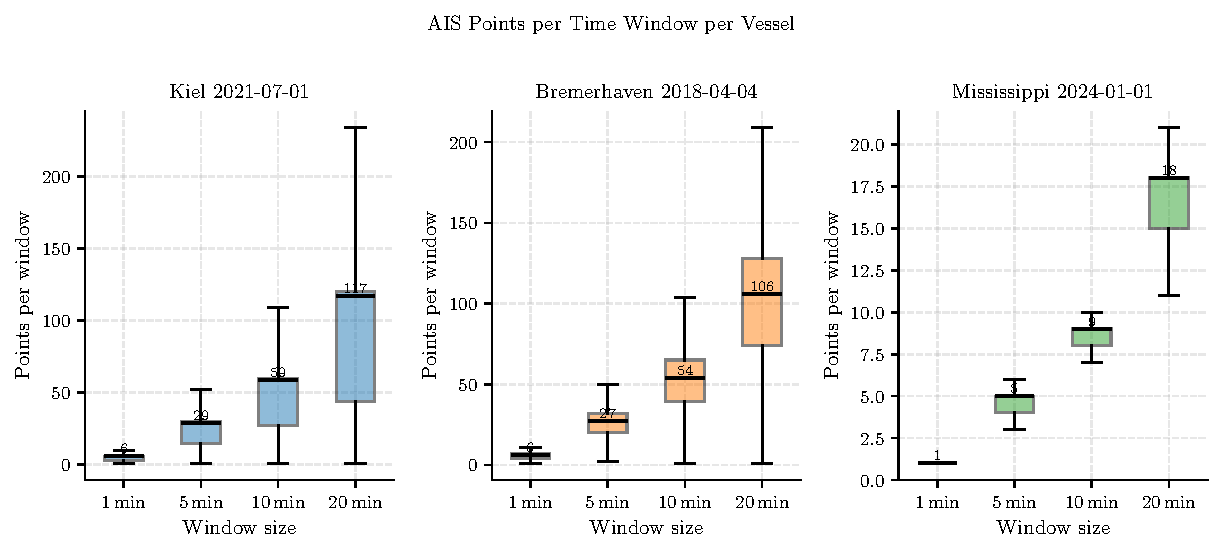
\includegraphics[width=1\textwidth]{figures/points_per_window.pdf}
\caption{Boxplot of AIS points per time window per vessel (sample day per dataset).}
\label{fig:points-per-window}
\end{figure}



\begin{figure}[ht]
\centering
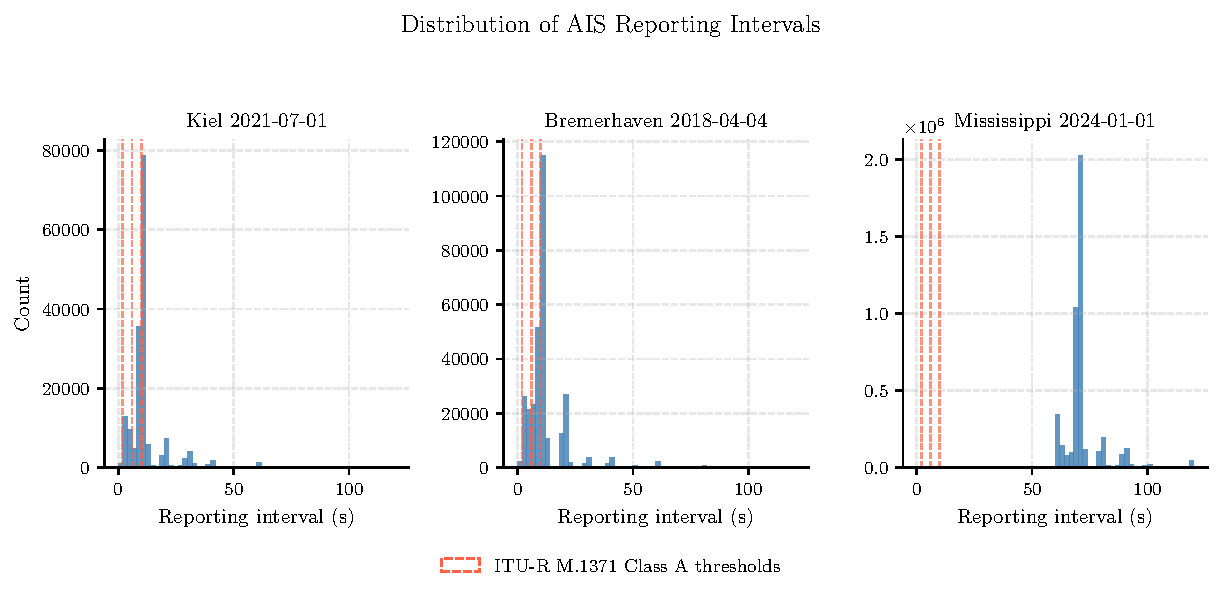
\includegraphics[width=1\textwidth]{figures/interval_hist.pdf}
\caption{Boxplot of inter-message intervals by velocity class.}
\label{fig:interval-hist}
\end{figure}

\begin{figure}[ht]
\centering
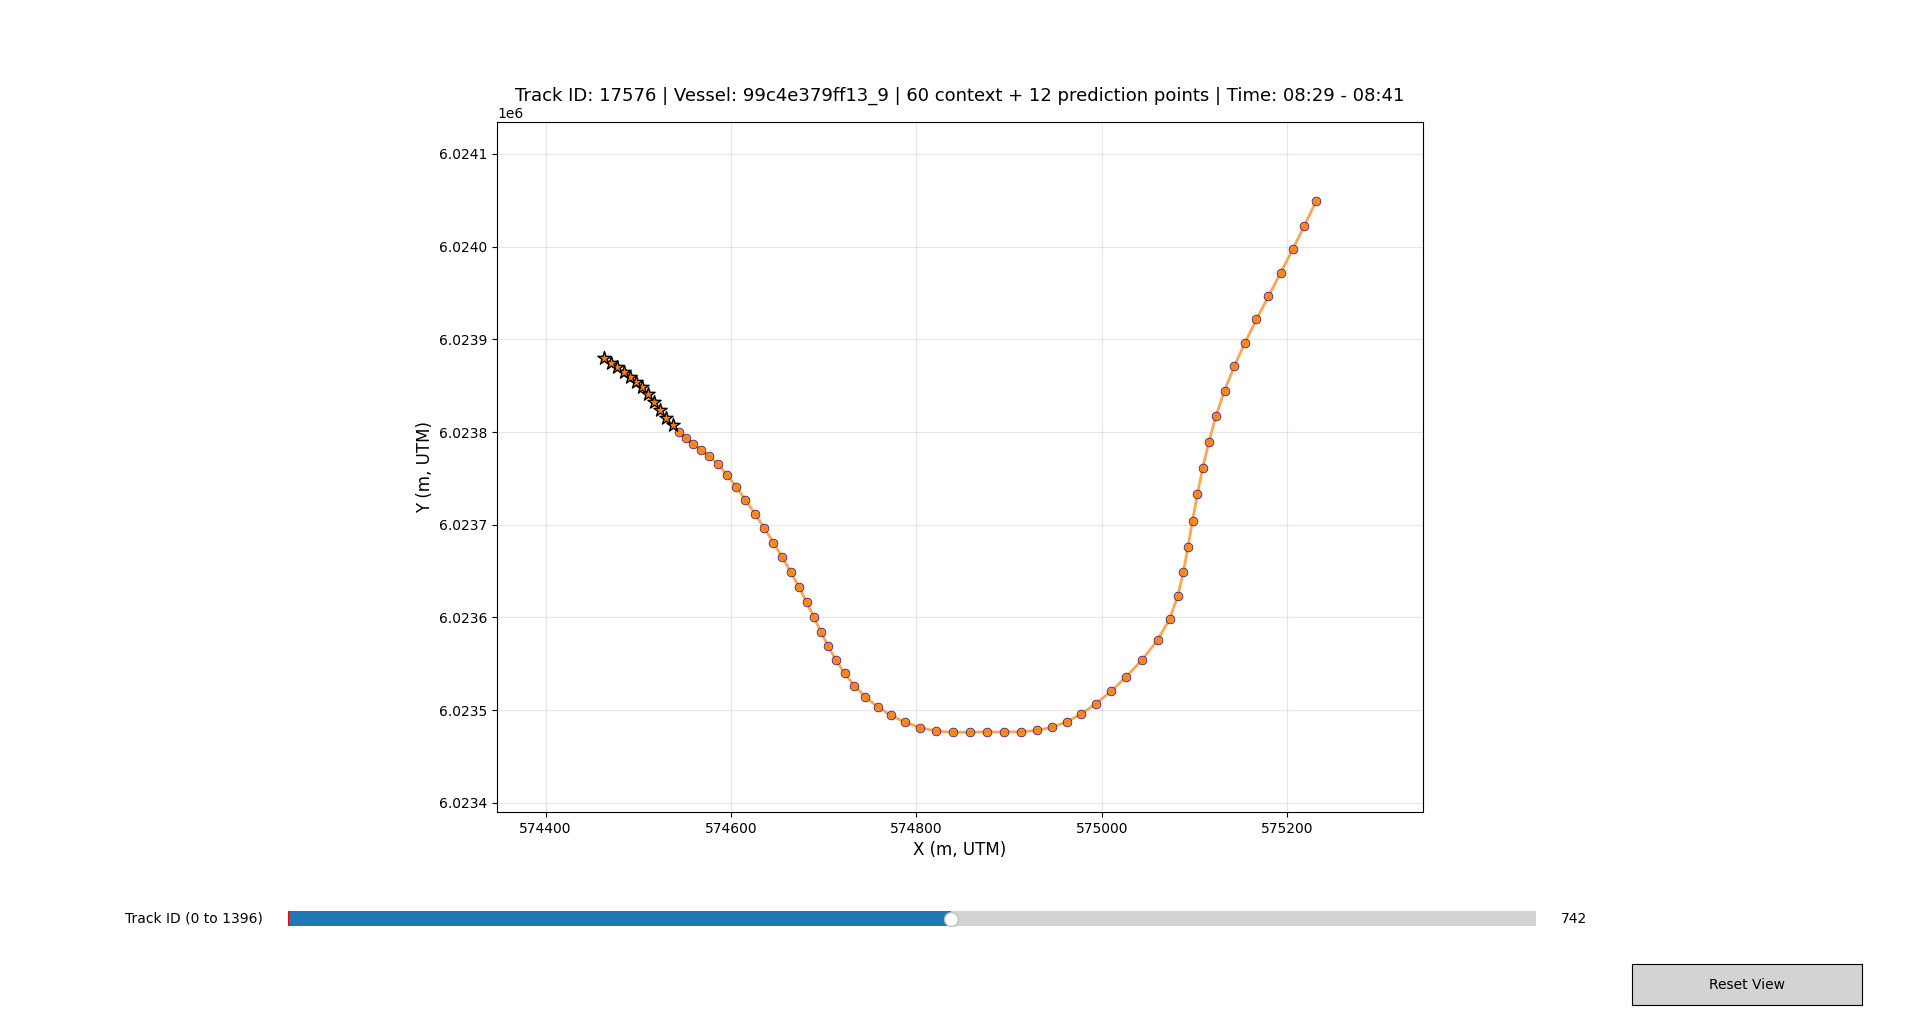
\includegraphics[width=1\textwidth, trim={9cm 3cm 9cm 2cm}, clip]{figures/kiel_trajectories_1.png}
\caption{Example training trajectory of Kiel Dataset. Circles depict Context, Stars Predictions}
\label{fig:sample-trajectory}
\end{figure}

\section{Limitations}
Despite the high fidelity of the processed datasets, several inherent limitations of the AIS system and the specific data sources must be acknowledged:
\subsubsection{Regulatory Reporting Bias}
The data primarily reflects the movement patterns of large commercial vessels mandated to carry Class A transponders under the International Convention for the Safety of Life at Sea (SOLAS) \cite{solas2014}. This includes cargo vessels exceeding 300,GT on international voyages and all tankers. Consequently, smaller recreational craft and fishing vessels utilizing Class B transponders are significantly underrepresented. Because Class B devices transmit at lower power and with less frequent update rates (as detailed in Section \ref{tab:ais-frequencies}), the resulting models may exhibit a bias toward the predictable, high-inertia dynamics of large commercial ships.


\subsubsection{Temporal Resolution and Information Loss}
The decision to use the NOAA Marine Cadastre dataset introduces a specific temporal constraint. While raw \ac{AIS} signals can be received at intervals as short as 2 seconds for fast-moving or maneuvering vessels, the NOAA archives are decimated to a fixed 60-second resolution to manage data volume \cite{noaa2025aisdict}. This reduction in sampling frequency creates a discrepancy between the German datasets (interpolated to 10,s) and the U.S. data. In high-speed scenarios or tight maneuvers, a 60-second interval may fail to capture the peak curvature of a trajectory, potentially leading to smoothing artifacts in the spline interpolation.

\todo{more? sensor noise? cheap sensors? note done if noticed in other literature}
\todo{Context labeling?}

%!TEX root=../main.tex
\chapter{Methodology}
\label{chap:methology}
\acresetall %reset abbrevations
%\todo{Anything that is related to how the experiments work should be moved. Anything related to the methods themselves (not related to experiments) should stay.}
%\me{4.1 and 4.2 are background, but you advised 1 lvl up. still feels out of place here}
%\todo{ Chapter 4 has a lot of content that belongs to Chapter 5, so I will read it when the content is moved in place. }
%\sug{guide: This section contains the methods used in this thesis. For example, details about the models and adversarial attacks.s}

 
In this chapter, we detail the methodological approach used to model vessel trajectories. We use Section \ref{sec:seq2seq} to establish the theoretical background required for sequence-to-sequence modelling and Section \ref{sec:automl} for the principles of \ac{AutoML}. In the subsequent sections \ref{sec:kinematicimplementation} to \ref{sec:sequenceimplementation}, we describe the exact definitions, state representations, and architectural configurations of the implemented models.
\ws{refer to sections explicitly using the ref command. First, you need to give them labels using label command.} 

\section{Sequence-to-Sequence Models}
\label{sec:seq2seq}
    %https://arxiv.org/html/2406.02770v1#bib.bib14

In the domain of Deep Learning, \acf{Seq2Seq}  Models \ws{they are usually called Seq2Seq, not S2S please modify} 
serve as a \ws{what does dependent sequences mean, elaborate} \me{rephrased, elaborated}
framework for tasks where both input and output take the form of ordered sequences, and the output sequence is conditioned on the input sequence as a whole. That is, each element of the output is not generated independently, but rather informed by the full context of the input (or previously generated outputs).
While \ac{Seq2Seq} is rooted in language processing tasks like translation \parencite{sutskever2014sequencesequencelearningneural}, it can be %dieses zitat vlt raus
applied to any kind of sequential data, ranging from numerical time series and sensor data to genomes and handwriting \parencite{gentleschmidt2019recurrentneuralnetworksrnns}. 
Most \ac{Seq2Seq} models are based on an Encoder-Decoder architecture. 
\ws{`Follow' an architecture is a rather strange expression. Models have architectures, they do not follow them.}
The Encoder processes the input sequence and compresses the information into a fixed-size context vector, typically called \ws{typically called}
the hidden state.
The Decoder uses this vector to generate the output sequence.
Often, this regeneration is implemented autoregressively, meaning only one time step \ws{time step}
is predicted at a time, multiple times in a row with a shifting context window.
\ws{Transition needed to the types of Seq2Seq models}
To implement the encoder and decoder components within this \ac{Seq2Seq} framework, an underlying architecture capable of processing ordered temporal data is required.

    \begin{comment} % zu ausführlich
        
    \begin{itemize}
        \item \textbf{Encoder}: Processes the input sequence and compresses the information into a fixed-size context vector (hidden state).
        \item \textbf{Decoder}: Uses this vector to generate the output sequence (e.g., the predicted GPS positions for the next 10 time steps).
    \end{itemize}
        \end{comment}

    %A graphical overview of Encoder Decoder Sequence Models using the following buidling blocks can be found in Figures \ref{fig:s2s_rnn_appendix}, \ref{fig:s2s_lstm_appendix}, \ref{fig:s2s_bilstm_appendix}, and \ref{fig:s2s_attention_appendix}:

    %Encoder and Decoder can for example be built with the following two building blocks:%bessere überleitung todo

    
\ws{Please convert these to paragraphs instead of subsections (or just in-line text) for both RNN and LSTM, and make them briefer. No need to get into the technical details of RNNs and LSTMs to this extent. You can write a brief version in the main paper and move the details to the appendix} 
\paragraph{RNNs and LSTMs.}
The core architecture for sequence-based learning is the \ac{RNN}.
The primary distinction between \acp{RNN} and conventional Feedforward Neural Networks is the direction of information flow.
Instead of a strictly forward pass, an \ac{RNN} utilises cycles to feed information back into the hidden state, which enables the incorporation of context from previous inputs.
As the sequence length increases, standard \acp{RNN} suffer from the vanishing gradient problem, which limits their capability to learn long-term dependencies.
To address this limitation, the \ac{LSTM} architecture was introduced.
The core innovation of the \ac{LSTM} is a cell state regulated by three gates. The forget, input, and output gates allow relevant information to persist across many time steps.
Furthermore, the architecture is mathematically equipped for multivariate sequence modelling. This allows the representation of non linear cross-channel correlations.
When implementing \acp{LSTM} within \ac{Seq2Seq} frameworks, several architectural configurations must be considered. 
Key design parameters include the number and direction of the hidden layers, as well as the choice of decoding strategy, which typically involves either a direct linear mapping or an autoregressive approach.
A more detailed mathematical description of the internal update processes for both \acp{RNN} and \acp{LSTM}, along with illustrations of the architectures can be found in Appendix \ref{appx: mathfoundations}.

   
    

    \begin{comment} % leider garnicht benutzt außer in related work, was diese mkapitel vorausgeht. wenn platz habe kann man wieder reinpacken
        
    \subsubsection{Bi-LSTM}
    Many variants and extensions of the \ac{LSTM} have been proposed to enhance its representative power. A notable architectural advancement is the \ac{Bi-LSTM}. While \cite{sutskever2014sequencesequencelearningneural} demonstrated that simply reversing the input sequence in a unidirectional \ac{Seq2Seq} model can significantly improve performance, the \ac{Bi-LSTM}, first introduced by \cite{articlebilstmorigins} formalizes this concept in its architecture .
    
    A \ac{Bi-LSTM} consists of two parallel hidden layers: a \textit{forward \ac{LSTM}} that processes the sequence in chronological order and a \textit{backward \ac{LSTM}} that processes it in reverse. Their respective hidden state outputs are then concatenated, added, averaged or multiplied  to form the final output. 
    Recent studies, such as \cite{articlebilstmsus} claim this makes the \ac{Bi-LSTM} more suitable for vessel trajectory prediction. 
   
    However, the application of \acp{Bi-LSTM} in autonomous systems and \ac{MTT} requires us to consider causality. Because the backward pass requires knowledge of the entire sequence up to the final time step, \acp{Bi-LSTM} are non-causal. Consequently, they cannot be used within the decoder of our \ac{Seq2Seq} Model. Nevertheless, they can be applied within the encoder stage. This allows the model to generate a richer input vector, which is then processed by a unidirectional decoder to predict future motion. %blabla als  hyperparameter in optimierer.. evtl auch schon hier den teil in methologie schreiben, mit tim klörne

      % 7 zusammenfassung: xlstm besser skalierbar, größerer speicher. aber für unsere 10 timesteps overkill. außerdem größerer feature space, schwerer (Schnell) manuell zu tunen, was unsere vorteile wettmachen würde + mangelnde vergeichbarkeit weil neu, . also nur kurz erklären
    %xlstm liefert die grundlage für ein lstm basiertes foundation modell durch erweiterung mit ..., aber dieses exisistiert leider noch nicht. wenn ich den platz habe würde ich gerne
    \end{comment}

    \paragraph{x-LSTM.} 
    \ws{please be consistent with . after the text in the paragraph. It is missing here and in other places in the thesis. Please check}
    Many variants and extensions of the \ac{LSTM} have been proposed.
    Recently, \textcite{beck2024xlstmextendedlongshortterm} introduced the \ac{x-LSTM} architecture to address bottlenecks of \ac{LSTM}. The primary goals of this architecture are to improve hardware scalability and to provide a larger memory capacity. To achieve this, two new \ac{LSTM} Layers are introduced:
    
    \begin{itemize}
        \item \textbf{\ac{s-LSTM}}: introduces exponential gating, which allows the model to revise and update its memory more dynamically.
        \item \textbf{\ac{m-LSTM}}: replaces the traditional vector cell state and its element-wise updates with a matrix memory updated via matrix multiplication. This %structural shift eliminates the sequential dependency of the hidden state, enabling 
        enables fully parallelised sequence processing during training.
    \end{itemize}
    Using these layers, an \ac{x-LSTM} can maintain the linear time complexity $\mathcal{O}(N)$ of conventional \acp{RNN} during inference, in contrast to the quadratic complexity of Transformers. \parencite{beck2024xlstmextendedlongshortterm, attentioniayn} %for respective Time omplexity 
    
    %However, the application of \ac{x-LSTM} in this work introduces practical challenges. 
    For our specific use case of predicting short 10-step trajectories, the expanded memory capacity offers limited benefits while introducing computational overhead. Furthermore, the architecture requires additional hyperparameters, such as the choice between \ac{s-LSTM} and \ac{m-LSTM} layers, as well as matrix dimensions. %number of heads.. aber die will ich hier nicht einführen
    This expands the search space for \ac{HPO} substantially.%, makes the tuning process computationally more expensive and harder to balance against simpler models. %Finally, as a recently proposed architecture, utilizing \ac{x-LSTM} would limit the comparability of our results with existing \ac{LSTM}-based maritime tracking approaches. 
    
    Nevertheless, because of it's scaling capabilities, the \ac{x-LSTM} builds the basis of the TiRex foundation model (Section \ref{subsec:foundation}).

\ws{The following can also be paragraphs instead of subsections}

\paragraph{Attention and Transformers.}
%ziemlcih kurz davor dass es sota ist, aber für uns ist hier alles gesagt, oder?
\ac{Seq2Seq} architectures based on \acp{RNN} or \acp{LSTM} face a structural limitation: The encoder must compress the entire input sequence into a single, fixed-size context vector. %, and information is lost. 
This compression creates an information bottleneck, causing the network to forget earlier parts of the sequence as the input length increases.  
\ws{This phrasing is not accurate. Now, you are claiming that because of compression, all `information' is lost. Also, the attention mechanism solved the `forgetting' problem rather than `lost' information. Please rephrase.} \me{added bottleneck}
To resolve this forgetting problem, \textcite{bahdanau2016neuralmachinetranslationjointly} introduced the attention mechanism.
Instead of relying on the final hidden state, attention allows the decoder to access all intermediate hidden states of the encoder. At each decoding step, the mechanism calculates an alignment score, which enables the model to assign higher weights to the timestamps most relevant to the current prediction.
Building upon this, \textcite{attentioniayn} proposed the Transformer architecture, which completely discards recurrent layers (such as \ac{RNN} or \ac{LSTM}) in favor of Self-Attention. 
Self-Attention computes the relational importance of all data points within a sequence simultaneously. This enables the models \ws{it does not allow `us'. We do not capture anything, the model does. Please rephrase}
to capture global dependencies.
%noch bischen umformulieren. filler weg un abschwächen evtl
However, applying Transformers to %short physical 
time series, such as our \ac{AIS} trajectories, presents new challenges. Unlike \acp{LSTM}, Transformers lack an inductive bias for sequential order and must rely on artificial positional encoding. 
A %recent 
critique by % in time series research 
\textcite{zeng2022transformerseffectivetimeseries} suggests that for short, physically continuous sequences where simple local dependencies dominate, Transformers can be unnecessarily complex, computationally expensive, and prone to overfitting compared to recurrent or linear models.
\ws{The citation should come at the end of the claim} \me{i resolved this by using singular with textcite.  i wanted to avoid making this sound like the source is a survey}.
Nonetheless, their capacity to parallelise efficiently has popularised Transformers as an architecture in large-scale predictive modelling. %needs citation ?
%\todo{factcheck skalierung}

\paragraph{Foundation Models.}
\label{subsec:foundation}
Because Transformers parallelise so effectively, they enabled the creation of Foundation Models. These are massive neural networks pretrained on vast, diverse datasets, across multiple domains such as weather, finance, and sensor data, to learn universal sequence patterns before being applied to a specific task. After being trained on very general data, they can be fine-tuned or adapted to specific tasks with relatively small amounts of task-specific data \parencite{Liang_2024foundation}.

A prominent example in time series forecasting is \textbf{Chronos} \parencite{ansari2024chronoslearninglanguagetime}, which tokenises time series values and processes them using a pure encoder architecture, or the more recent adaption \textbf{Chronos-2} \parencite{ansari2025chronos2}, which uses group attention to maintain weights across channels and enable multivariate or covariate informed forecasting. For our vessel trajectory prediction, Foundation Models offer two  application paradigms:
\begin{itemize}
    \item \textbf{Zero-Shot Forecasting:} The pretrained model generates predictions for \ac{AIS} trajectories without ever having been trained on maritime data. Chronos in particular was developed to  have comparable and occasionally superior zero-shot performance on new datasets, relative to methods that were trained specifically on them \parencite{ansari2024chronoslearninglanguagetime}.
    \item \textbf{Fine-Tuning (Warm Starting):} The model is can be trained on our specific domain data. By initialising \ws{british english}
    the training process with pretrained weights (a \enquote{warm start}) rather than random initialisation, the model requires significantly less domain data and computational time to adapt to the specific kinematics of inland vessels. %\me{we dont do that. still include the possibility?}
\end{itemize}% \me{only did zero shot, shorten?}

%While Transformer based foundation models represent the current state-of-the-art in generalized forecasting, they come with computational overhead. %wieso habe ich das geschreiben, das ist ja nur inferenz

The \ac{x-LSTM} architecture \parencite{beck2024xlstmextendedlongshortterm} addresses the  \ws{cannot use possesive s with inanimate} 
lack of sequential bias of the Transformer while maintaining extreme scalability. %O(N) in lstm anzahl layer vs O(n^2) für Transformer as mentioned before
Consequently, \acp{x-LSTM} provide the theoretical basis for \ac{RNN}-based Foundation Models. 
The \textbf{TiRex} foundation model,
%One very recent foundation model, \textbf{TiRex},
\ws{no need to mention very recent. These expressions are reserved to `related work'} 
 which leverages the \ac{x-LSTM}, was presented by \textcite{auer2025tirexzeroshotforecastinglongtrex} and showed promising results in benchmarks against Chronos. However, the authors have noted the model does not perform well with multivariate times eries data. As a consequence, applicability to \ac{AIS} Trajectories is limited \ws{is limited ... then give reasons.}
, because the univariate model treats individual features as independent channels, which prevents it from capturing cross-correlations. Since vessel dynamics are governed by physical constraints where \ac{SOG} and \ac{COG} directly impact the trajectory, this approach may result in kinematically inconsistent predictions.

\ws{Never use future tense for completed work. The future tense is only use when you write a plan}    
We will benchmarked our self-trained \ac{LSTM} model against Chronos-2 and TiRex to both investigate whether generalised, pretrained knowledge outweighs physically grounded, domain-specific recurrence, and test zero shot performance of \ac{x-LSTM} based foundation model vs Transformer based.
    

\section{Automated Machine Learning}
%todo some rephrasing, more details on hyperband, explain cash similar level to hpo

\label{sec:automl}

The development of machine learning applications traditionally relies on human intervention and domain expertise.
\ac{AutoML} aims to reduce the manual effort and knowledge required by automating design choices.
These choices include decisions regarding model architecture, evaluation, and optimisation \parencite{hutter2019automated}.
The primary goal of \ac{AutoML} is to make machine learning accessible to non-experts, while also accelerating the development process for experienced ML-engineers by removing repetitive tasks \parencite{AutoMLHoos, hutter2019automated}.
The automated configuration of a machine learning model is fundamentally defined by three core components.
First, a search space must be established to set the boundaries of all permissible model configurations.
Second, a search strategy is required to systematically navigate this multidimensional space and identify promising candidates.
Finally, we need to define performance estimation methods to evaluate the sampled configurations.
In this work, \ac{AutoML} is utilised specifically for \ac{HPO}, as detailed in Section \ref{subsec:automlhpo}.s
 The concepts of search spaces and search strategies are covered in the following subsections \ref{subsec:search_space} and \ref{subsec:searchstrat}. The methodology for performance evaluation is addressed separately within Chapter \ref{chap:experimentalsetup}.
\ws{Too many details in this secion as well. You can mention briefly the methods you used and move the deep details to the appendix. Examples, no need to explain how BO works in the main thesis content.}
\ws{No transition here. You mentioned steps then jumped to something called `the search space'. You need a transition here. Example, remove the steps and mention the components of AutoML instead, then explain them one by one in subchapters (as it is now)}. \me{did a rewrite of this section. content moved to appendix and chatper 5, intro and transitions adjusted}

\subsection{The Search Space}
\label{subsec:search_space}

The foundation of any \ac{AutoML} problem is the definition of its search space. WIth the search space, we set the boundaries of the automated system and define the set of all possible configurations that the optimiser is allowed to explore to find the configuration with the best performance.

\paragraph{Hyperparameter Optimisation.}
\label{subsubsection:HPO}
Hyperparameters control the learning process of a model, but they cannot be derived from training data via standard gradient-based optimisation.
As a result, they must be set prior to training \parencite{hutter2019automated}.
In \ac{HPO}, the search space is restricted to the hyperparameters of a single, predefined learning algorithm.
These parameters can be continuous, integer-valued, or categorical.

\paragraph{Model Selection.}
Model selection is applied at a higher level of abstraction than \ac{HPO}.
Instead of tuning the internal mechanics of a specific algorithm, the search space consists of a discrete set of different machine learning algorithms to identify the algorithm family that best models the underlying data distribution.




\paragraph{CASH Problem.}
In practice, model selection and \ac{HPO} are intertwined, because the optimal hyperparameters depend entirely on the chosen algorithm.
This interdependency is formulated as the \ac{CASH} problem.
When formulating \ac{CASH} as a single, joint optimisation problem, the search space grows exponentially.
The combination of discrete algorithm choices with their respective continuous, discrete, and categorical hyperparameters presents a massive computational challenge.
Consequently, solving the \ac{CASH} problem efficiently typically requires meta-learning or a warm start, where metadata and historical performance records from previously evaluated datasets are utilised \parencite{AutoMLHoos}.
Because such extensive metadata is not available for the specific inland vessel trajectories utilised in this work, addressing the full \ac{CASH} problem is computationally unfeasible.
A detailed mathematical formalisation of \ac{HPO}, model selection, and the \ac{CASH} problem is provided in Appendix \ref{app:math_search_space}.

\paragraph{NAS Problem.} \me{can i delete this paragraph? only mentioned here to give a full picture of automl)}
\acf{NAS} expands the search space even further by fully automating the design of the neural network architecture itself. Instead of selecting predefined algorithms, \ac{NAS} optimises the arrangement of operations, layer connectivity, and network depth \parencite{AutoMLHoos}. Due to the immense size of the resulting search space, \ac{NAS} requires unfeasable computational resources and falls out of scope for this thesis. In practice, \ac{NAS} is typically only applied once the fundamental type of layer (e.g., \ac{LSTM} or Transformer) has already been established.


\begin{comment} %sompressed and moved details to appendix
    
The development of machine learning applications traditionally relies on human intervention and domain expertise. \ac{AutoML} aims to reduce the manual effort and knowledge required by automating design choices. Those choices include decisions regarding model architecture, evaluation, and optimisation \parencite{hutter2019automated}. The primary goal of \ac{AutoML} is to make machine learning accessible to non-experts, while also accelerating the development process for experienced ML-engineers by removing repetitive tasks \parencite{AutoMLHoos, hutter2019automated}.

Analogous \ws{do you mean analogous?} \me{yes :)}
to the traditional pipeline, a complete \ac{AutoML} pipeline can be broadly categorised into the following stages:
\begin{itemize}
    \item \textbf{Data Preparation and Feature Engineering:} Automatically cleaning raw data, imputing missing values, and constructing or selecting relevant features.
    \item \textbf{Model Selection:} Choosing the appropriate mathematical model or algorithm family for the given dataset.
    \item \textbf{\ac{HPO}:} Tuning the configuration parameters that control the learning process of a selected model.
\end{itemize}
\ws{This sentece is out of place}
In this work, \ac{AutoML} was used for \ac{HPO}, as detailed in Section \ref{subsec:automlhpo}. 
\ws{until here} \me{put back below the enumeration. this takes up more space unfortunately}
%In this work, \ac{AutoML} was used for \ac{HPO}, as detailed in Section \ref{subsec:automlhpo}. spart mir eine zeile

\ws{No transition here. You mentioned steps then jumped to something called `the search space'. You need a transition here. Example, remove the steps and mention the components of AutoML instead, then explain them one by one in subchapters (as it is now)}.
\subsection{The Search Space}
\ws{use title case in the titles} \me{applied everywhere}
The foundation of any \ac{AutoML} problem is the definition of its search space. This space sets the boundaries of the automated system and defines the set of all possible configurations that the optimiser is allowed to explore to find the configuration with the best performance.

\paragraph{Hyperparameter Optimisation.}
\label{subsubsection:HPO}

Hyperparameters control the learning process of a model but, unlike model parameters (weights), cannot be derived from training data via standard gradient-based optimisation. As a result, we need to set them prior to training \parencite{hutter2019automated}. \ac{HPO} restricts the search space to the hyperparameters of a single, predefined learning algorithm.

\ws{Too many details in this secion as well. You can mention briefly the methods you used and move the deep details to the appendix. Examples, no need to explain how BO works in the main thesis content.}
\me{überlegen was alles ins appendix kann und wie ich das dann strukturiere. BO ist schon weg. next: 4.2.1 mathe in anhang4.5.2 in experiment teilweise. rest nur auf nachfrage}

Formally, adapted from \textcite{AutoMLHoos} to reflect the fixed training and validation split we use, we can let $A_\lambda$ denote a learning algorithm $A$ instantiated with hyperparameter configuration $\lambda \in \Lambda$, where $\Lambda$ is the
hyperparameter search space. Given a dataset $\mathcal{D}$ split into a training set $\mathcal{D}_\text{train}$ and a validation set
$\mathcal{D}_\text{val}$, the \ac{HPO} objective is:
\begin{equation*}
    \lambda^* = \underset{\lambda \in \Lambda}{\arg\min}\;
    \mathcal{L}\!\left(A_\lambda,\, \mathcal{D}_\text{train},\,
    \mathcal{D}_\text{val}\right)
    \label{eq:hpo}
\end{equation*}
where $\mathcal{L}$ is a validation loss metric. Since evaluating $\mathcal{L}$ requires fully training $A_\lambda$, each function evaluation is expensive, and \ac{HPO} is a black-box optimisation problem.

Hyperparameters can be of several types, which together determine the structure of $\Lambda$, such as:
\begin{itemize}
    \item \textbf{Continuous:} Real-valued parameters such as the learning
    rate or regularisation strength. They are typically searched on a
    log-uniform scale.
    \item \textbf{Integer-valued:} Discrete but ordered parameters, such as
    the number of hidden units or the sequence input length.
    \item \textbf{Categorical:} Unordered discrete choices, such as the
    type of optimiser, the activation function or the set of input features.
    %\item \textbf{Conditional:} Parameters that are only relevant given a
    %specific value of another hyperparameter. For example, the dropout rate
    %is only meaningful if a dropout layer is included in the architecture.
    %Conditional hyperparameters introduce a hierarchical structure into
    %$\Lambda$, commonly represented as a \emph{configuration space}
    %\parencite{hutter2019automated}.
\end{itemize}





\paragraph{Model Selection.}
Model Selection operates at a higher level of abstraction than \ac{HPO}. Instead of tuning the internal mechanics of a specific algorithm, the search space consists of a discrete set of different machine learning algorithms $\mathcal{A} = \{A^{(1)}, \dots, A^{(R)}\}$ (e.g., \ac{LSTM} vs. Transformer). The objective is to identify the algorithm family that best models the underlying data distribution. 


Formally, adapted from \textcite{AutoMLHoos} to reflect the fixed training and validation split we use%rather than $k$-fold cross-validation
, the algorithm selection problem can be defined as finding the algorithm $A^* \in \mathcal{A}$ that yields the best performance on the validation set:
\begin{equation*}
    A^* = \underset{A \in \mathcal{A}}{\arg\min}\;
    \mathcal{L}\!\left(A,\, \mathcal{D}_\text{train},\,
    \mathcal{D}_\text{val}\right)
    \label{eq:model_selection}
\end{equation*}
%Because one of our deliverables is a model comparison, Model selection is not used for the thesis, as in a \ac{CASH} Problem, not every model is evaluated at it's full capability. das war mir nicht präzise genug. müsste man genau reindiven aber ist auch irrelevant wenn keiner danach fragt

\paragraph{CASH Problem.}
In practice, Model Selection and \ac{HPO} are intertwined: the optimal hyperparameters depend entirely on the chosen algorithm, and the true potential of an algorithm can only be evaluated if its hyperparameters are properly tuned. \textcite{hutter2019automated} formulate this interdependency as the \acf{CASH} problem.%: Combined Algorithm Selection and Hyperparameter optimisation. 

Formally, again adapted from \textcite{AutoMLHoos} to reflect the fixed training and validation split, given a set of learning algorithms $\mathcal{A}$, where each algorithm $A^{(j)} \in \mathcal{A}$ has an associated hyperparameter configuration space $\Lambda^{(j)}$, the \ac{CASH} problem seeks to jointly find the optimal algorithm $A^*$ and its optimal hyperparameter configuration $\lambda^*$:% \parencite{AutoMLHoos}:
\begin{equation*}
    A^*, \lambda^* = \underset{A^{(j)} \in \mathcal{A},\, \lambda \in \Lambda^{(j)}}{\arg\min}\;
    \mathcal{L}\!\left(A^{(j)}_\lambda,\, \mathcal{D}_\text{train},\,
    \mathcal{D}_\text{val}\right)
    \label{eq:cash}
\end{equation*}

When formulating \ac{CASH} as a single, joint optimisation problem, the search space grows exponentially. Combining the discrete choices of algorithms with their respective continuous, discrete, and categorical hyperparameters creates a massive computational challenge. Typically, solving the \ac{CASH} problem efficiently requires meta-learning or a \emph{warm start}, which uses metadata and historical performance records from previously evaluated datasets \parencite{AutoMLHoos}. Because such extensive metadata is not available for the specific inland vessel trajectories utilised in this work, addressing the full \ac{CASH} problem is computationally unfeasible for this thesis. %in methologie?


\paragraph{NAS Problem.} \me{can i delete this? only mentioned here to give a full picture of automl)}
\acf{NAS} expands the search space even further by fully automating the design of the neural network architecture itself. Instead of selecting predefined algorithms, \ac{NAS} optimises the arrangement of operations, layer connectivity, and network depth \parencite{AutoMLHoos}. Due to the immense size of the resulting search space, \ac{NAS} requires unfeasable computational resources and falls out of scope for this thesis. In practice, \ac{NAS} is typically only applied once the fundamental type of layer (e.g., \ac{LSTM} or Transformer) has already been established.

\end{comment}
\subsection{Search Strategies and Pruning}
\label{subsec:searchstrat}
Once a search space is defined, the \ac{AutoML} system requires a strategy to navigate it. Standard search strategies include Grid Search, which evaluates all predefined combinations, and Random Search, which samples configurations uniformly at random. While Random Search is generally more efficient in high-dimensional spaces, %whose performance function has low effective dimensionality
both methods are uninformed and do not utilise past evaluations to guide future selections \parencite{hutter2019automated}. Advanced, informed strategies, such as \acf{BO} , build a probabilistic surrogate model of the objective function to sample only the most promising regions of the search space. %kept this the same
%As an informed search strategy, \ac{BO} builds a probabilistic surrogate model of the objective function to predict the performance of unseen hyperparameter configurations.
Traditional \ac{BO} approaches relying on Gaussian Processes model the probability of the objective value given the hyperparameters directly \parencite{hutter2019automated}.
This direct approach becomes computationally expensive as the number of evaluations grows and scales poorly in high-dimensional configuration spaces \parencite{hutter2019automated}. Moreover, Gaussian process based \ac{BO} cannot natively handle mixed hyperparameter spaces and requires approximations to evaluate categorical variables \cite{AutoMLHoos}. 
To address these limitations, we used the \ac{TPE} algorithm \parencite{bergstra2011algorithms} in this work.
Rather than modelling the objective function directly, the \ac{TPE} inverts the process by modelling the probability of the hyperparameters given the objective value, partitioning past observations into sets of good and bad configurations.
This inversion provides a significant advantage for tuning complex sequence models, as the primary strength of the \ac{TPE} lies in its robust handling of discrete and categorical hyperparameters \parencite{AutoMLHoos}.
Furthermore, each iteration of the algorithm scales linearly with the number of hyperparameters.
A more detailed technical description of \ac{BO} and the \ac{TPE} algorithm is provided in Appendix~\ref{appx:BOandTPE}.

Search strategies are frequently paired with pruning mechanisms.
Through pruning, or early stopping, the training of unpromising configurations is terminated before the maximum allocated budget is consumed.
In methods such as Successive Halving, a large number of configurations are evaluated for a few epochs, the worst-performing candidates are discarded, and more computational resources are allocated to the top performers.

% ----------------------------------------------------------------------
\begin{comment} %moved to appendix
    
Once a search space is defined, the \ac{AutoML} system requires a strategy to navigate it. Standard search strategies include Grid Search, which evaluates all predefined combinations, and Random Search, which samples configurations uniformly at random. While Random Search is generally more efficient in high-dimensional spaces, %whose performance function has low effective dimensionality
both methods are uninformed and do not utilise past evaluations to guide future selections \parencite{hutter2019automated}. Advanced, informed strategies, such as \acf{BO} , build a probabilistic surrogate model of the objective function to sample only the most promising regions of the search space. 


\paragraph{Bayesian Optimisation.}
\acf{BO} uses past evaluations to make informed decisions about which hyperparameters to test next \parencite{hutter2019automated}. This is critical for models where evaluating the true objective function $\mathcal{L}$ is computationally expensive (i.e., fully training an \ac{LSTM}). %lstm example not covered by hutteretal

\ac{BO} achieves this by constructing a probabilistic surrogate model $\hat{f}$, which approximates the true, expensive loss function based on all previously evaluated configurations. Because the surrogate model $\hat{f}$ is cheap to evaluate, the optimiser can test more potential configurations internally to identify the most promising candidates before committing resources to a full model training.

To decide which configuration to evaluate next based on the given surrogate model, \ac{BO} relies on an acquisition function. A commonly used acquisition function is \acf{EI} \parencite{AutoMLHoos}. \ac{EI} evaluates a candidate by combining two essential terms: the expected value of the function at a given point, and the associated variance %, or uncertainty %also covered by automlhoos. jsut wanted to assosiate it earlier
. This combination provides a trade-off between two competing goals:
\begin{itemize}
    \item \textbf{Exploitation:} By considering the expected value, the search is focused on promising regions of the search space that contain good candidate solutions with high probability.
    \item \textbf{Exploration:} In contrast, the variance term encourages the exploration of unknown areas that are weakly explored, or where candidate solutions of highly variable quality have been observed \parencite{Jones1998}.%, AutoMLHoos}. \me{Das ist ein Sekundärzitat, nachfragen}
    %\me{I was unsure how to handle citations here. Jones is the original source, found in AutoMLHoos. i read both. we talked about it}
\end{itemize}
Figure~\ref{fig:bo_illustration} illustrates one iteration of this process. %published as open acces. Open access works published by Springer Nature are published under Creative Commons licences.tdoo resolved (check licensing, otherwise use the one from the literature overview automl timeseries)

\begin{figure} [h]
    \centering
    % Adjust trim values (left bottom right top) 
    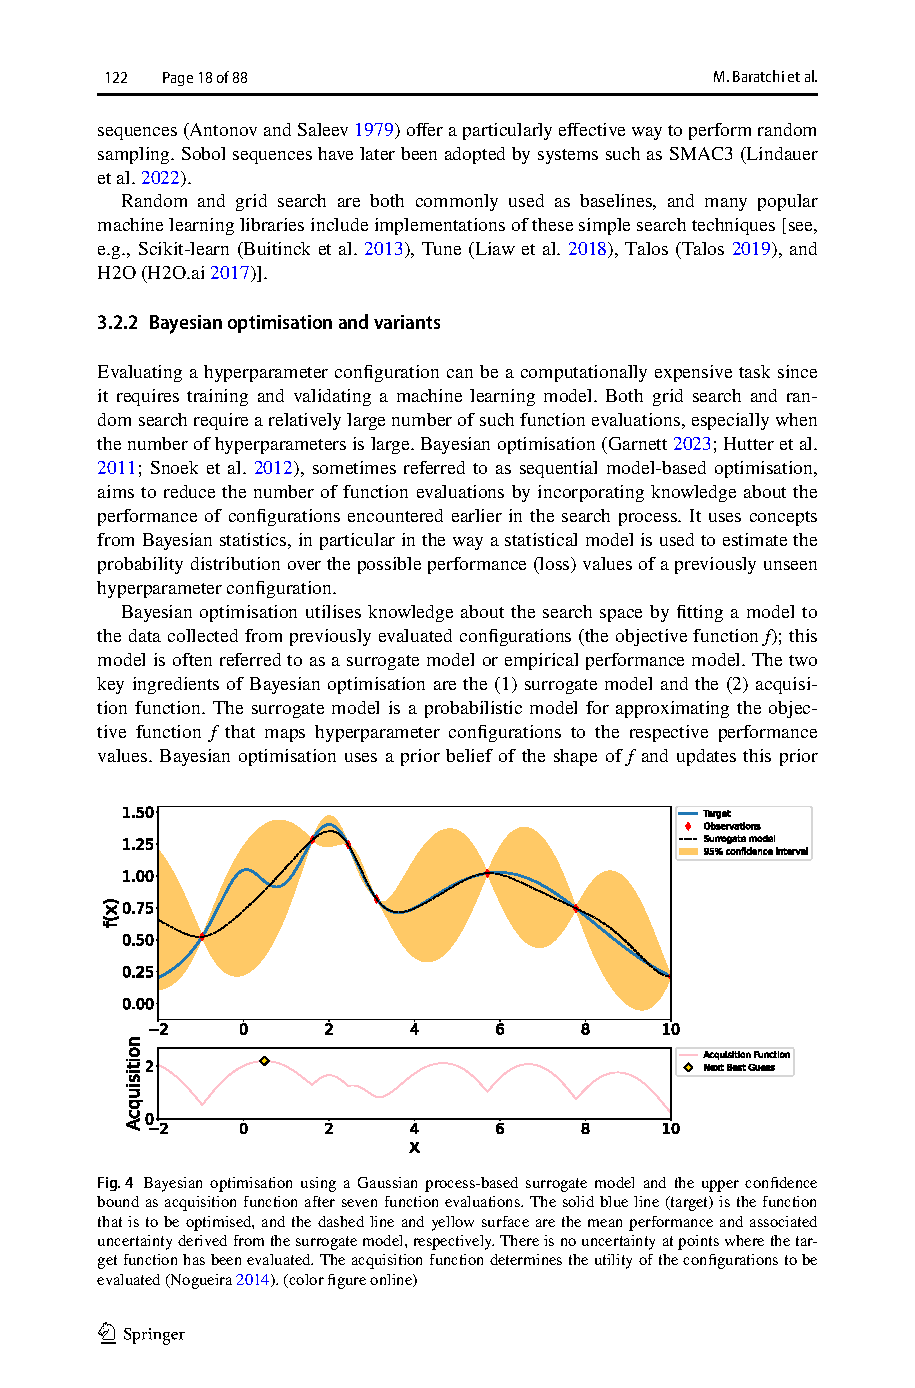
\includegraphics[width=0.8\linewidth,trim={2cm 4cm 2cm 13.5cm}, clip]{figures/985693BO.pdf}
    \caption[Bayesian Optimisation]{\acf{BO} using a surrogate model and \acf{EI} after several evaluations. The solid line represents the true objective $\mathcal{L}$, the dashed line and shaded region show the surrogate mean and 95\% confidence interval, respectively. The acquisition function (bottom) determines the next candidate configuration to evaluate \parencite{AutoMLHoos}.}
    \label{fig:bo_illustration}
\end{figure}

%Common algorithms used as surrogate models include \emph{Gaussian Processes} and \emph{Random Forests}. While Gaussian Processes provide good uncertainty estimates for continuous parameters, Random Forests are often preferred in \ac{AutoML} frameworks such as \ac{SMAC}, because they scale more efficiently and natively handle discrete and categorical hyperparameters \parencite{AutoMLHoos}. \me{maybe delete paragraph, irrelevant. also maybe dont explain Ei if i dont use it, but i think its fine as a baseline}
While classical\ac{BO} surrogate models such as Gaussian Processes model $p(y \mid \lambda)$ directly, they can scale poorly with the number of hyperparameters and struggle with discrete and categorical parameters.

\paragraph{Tree-Structured Parzen Estimator.} 
The \ac{TPE} \parencite{bergstra2011algorithms} addresses these limitations of \ac{BO} by inverting the modelling problem. This enables better handling of categrical hyperparameters. Rather than directly modelling $p(y \mid \lambda)$, the \ac{TPE} instead constructs two separate density functions, $p(\lambda \mid y < \alpha)$ and $p(\lambda \mid y \geq \alpha)$. The threshold $\alpha$ partitions all observations into a set of good and bad configurations, each of which is modeled using one-dimensional Parzen windows. 
Parzen windows are kernel density estimators that place a smooth Gaussian function at each data point, with their sum forming the density function.
 The ratio $\frac{p(\lambda\mid y \ge \alpha)}{p(\lambda\mid y < \alpha)}$ is closely related to the expected improvement acquisition function and serves as the criterion for proposing new hyperparameter configurations \parencite{bergstra2011algorithms, hutter2019automated}. \ac{TPE} further scales linearly with the number of hyperparameters \parencite{AutoMLHoos}. %Through maintaining a sorted list of confgurations in memory, 
\me{ probably replace BO graphic with the TPE figure i made for the defense}

\end{comment}


%%%%%%%%%%%%%%%%%
\ws{Please move the full text to the chapter tex file. This reference is just extra complication with no benefits}

%
%!TEX root=../main.tex
\chapter{Background} %7-10 pages, will be  hard  to do lesss
\label{chap:background}

\section{Trajectory prediction in maritime/AIS}%core SOTA
\section{Motion Models} \todo{fill once I implemented them}
    \subsection{CV}
    %\subsection{CA}
    \subsection{CTRV}
    %\subsection{IMM?} ich denke nicht, darauf  soll der fokusnicht liegen
\section{Sequence-to-Sequence Models}   
    %https://arxiv.org/html/2406.02770v1#bib.bib14

  \todo{graphics in universal style. They do not help me a lot personally, so I did not include them yet}

    In the domain of Deep Learning, \ac{S2S}  Models serve as a framework for tasks where input and output are dependent sequences. While \ac{S2S} is rooted in language processing tasks like translation \cite{sutskever2014sequencesequencelearningneural}, it can be %dieses zitat vlt raus
    applied to any kind of sequential data, ranging from numerical time series and sensor data to genomes and handwriting \cite{gentleschmidt2019recurrentneuralnetworksrnns}. 
    Most \ac{S2S} models follow an \textbf{Encoder-Decoder} architecture. 
    \begin{itemize}
        \item \textbf{Encoder}: Processes the input sequence and compresses the information into a fixed-size context vector (hidden state).
        \item \textbf{Decoder}: Uses this vector to generate the output sequence (e.g., the predicted GPS positions for the next 10 time steps).
    \end{itemize}
    Encoder and Decoder can for example be built with the following two building blocks:%bessere überleitung todo

    \subsection{RNN}
    Building on the first popular model to use recurrence, the Hopfield Network introduced by \cite{hopfieldrnn}, the foundational concept for sequence-based learning is the \ac{RNN}. 
    The primary distinction between \acp{RNN} and conventional Feedforward Neural Networks, such as \acp{MLP}, is the direction of information flow. While Feedforward Networks are acyclic, \acp{RNN} use cycles to feed information back into the hidden state, the \textit{memory}. This architecture allows the model to incorporate historical context from previous inputs $X_{0:t-1}$ when processing the current input $X_t$, rather than treating each input in isolation \cite{gentleschmidt2019recurrentneuralnetworksrnns} and to make decisions based on the patterns it recognizes \cite{AIBook}. The recurrence can be expressed as:

    \begin{equation}
        H_t = \phi_h (X_t W_{xh} + H_{t-1} W_{hh} + b_h) % liefert eigentlich keinen mehrwert
    \end{equation}
    where $W$ represents weight matrices and $\phi$ an activation function. Despite their theoretical capability to handle sequences, \acp{RNN} suffer from the \textit{vanishing gradient problem}, as well as the \textit{exploding gradient problem}, as has been established by \cite{279181bengio}. As the sequence length increases, the gradients used to update weights during backpropagation decrease exponentially, preventing the model from learning long-term dependencies.
    %wenn gefragt, für eine kurze definition der PRobleme, \cite{AIBook}
    
    \subsection{LSTM}
     To address the limitations of standard \acp{RNN} in capturing long-term dependencies, \cite{hochreiterLSTM} introduced the \ac{LSTM} architecture. The core innovation of the \ac{LSTM} is the introduction of a cell state $C_t$, which allows information to persist across many time steps. The flow of information in and out of these cells is regulated by three \textbf{gates}: The
    \begin{itemize}
        \item \textbf{Forget Gate $F_t$}:  Determines which information from the previous cell state $C_{t-1}$ is no longer needed and should be discarded.
        \item \textbf{Input Gate $I_t$}: Decides which new information from the current input $X_t$ and previous hidden state $H_{t-1}$ is relevant to be stored in the cell state.
        \item \textbf{Output Gate $O_t$}: Controls which parts of the current cell state $C_t$ are used to compute the new hidden state $H_t$.
    \end{itemize}
    
     Following the formalization by \cite{gentleschmidt2019recurrentneuralnetworksrnns}, the internal update process is defined by the following set of equations:
     \begin{align}
         F_t &= \sigma(X_t W_{xf} + H_{t-1} W_{hf} + b_f) \\%forget
         I_t &= \sigma(X_t W_{xi} + H_{t-1} W_{hi} + b_i) \\%input
         \tilde{C}_t &= \tanh(X_t W_{xc} + H_{t-1} W_{hc} + b_c) \\%input candidate
         C_t &= F_t \odot C_{t-1} + I_t \odot \tilde{C}t \\ % update by multiplying old with forget and adding new
         O_t &= \sigma(X_t W{xo} + H_{t-1} W_{ho} + b_o) \\ %output: which part of memory is relevant?
         H_t &= O_t \odot \tanh(C_t)
     \end{align}
     
     In these equations, $\tilde{C}_t$ represents a candidate cell state, $\sigma$ is the sigmoid activation function $\sigma(x) = \frac{1}{1 + e^{-x}}$, and $\odot$ denotes the element-wise (Hadamard) product. By using an this update for the cell state $C_t$, the \ac{LSTM} prevents the gradient from vanishing as quickly as in standard \acp{RNN}, allowing the network to learn relationships across significantly larger time gaps.

     As indicated by the multi-dimensional input vector $X_t$ and the associated weight matrices, the \ac{LSTM} architecture is mathematically equipped for multivariate sequence modeling. The model has the capacity to represent nonlinear cross-channel correlations, because the internal gating mechanisms integrate information from all input features simultaneously to model their interdependencies within a shared hidden representation, making it suitable for our usecase. 
     %achtung (für methodik:) LSTM erwarten gleichbleibende frequenz, informationsverlust durch interpolieren
    

    \subsubsection{Bi-LSTM}
    Many variants and extensions of the \ac{LSTM} have been proposed to enhance its representative power. A notable architectural advancement is the \ac{Bi-LSTM}. While \cite{sutskever2014sequencesequencelearningneural} demonstrated that simply reversing the input sequence in a unidirectional \ac{S2S} model can significantly improve performance, the \ac{Bi-LSTM} formalizes this concept in its architecture.
    
    A \ac{Bi-LSTM} consists of two parallel hidden layers: a \textit{forward \ac{LSTM}} that processes the sequence in chronological order and a \textit{backward \ac{LSTM}} that processes it in reverse. Their respective hidden state outputs are then concatenated, added, averaged or multiplied  to form the final output. 
    Recent studies, such as \cite{articlebilstmsus} claim this makes the \ac{Bi-LSTM} more suitable for vessel trajectory prediction. 
   
    However, the application of \acp{Bi-LSTM} in autonomous systems and \ac{MTT} requires us to consider causality. Because the backward pass requires knowledge of the entire sequence up to the final time step, \acp{Bi-LSTM} are non-causal. Consequently, they cannot be used within the decoder of our \ac{S2S} Model. Nevertheless, they can be applied within the encoder stage. This allows the model to generate a richer input vector, which is then processed by a unidirectional decoder to predict future motion. %blabla als  hyperparameter in optimierer.. evtl auch schon hier den teil in methologie schreiben, mit tim klörne

      % 7 zusammenfassung: xlstm besser skalierbar, größerer speicher. aber für unsere 10 timesteps overkill. außerdem größerer feature space, schwerer (Schnell) manuell zu tunen, was unsere vorteile wettmachen würde + mangelnde vergeichbarkeit weil neu, . also nur kurz erklären
    %xlstm liefert die grundlage für ein lstm basiertes foundation modell durch erweiterung mit ..., aber dieses exisistiert leider noch nicht. wenn ich den platz habe würde ich gerne

    \subsubsection{x-LSTM}

    Recently, \cite{beck2024xlstmextendedlongshortterm} introduced the \ac{x-LSTM} architecture to address bottlenecks of \ac{LSTM}. The primary goals of this architecture are to improve hardware scalability and to provide a larger memory capacity. To achieve this, two new \ac{LSTM} Layers are introduced:
    
    \begin{itemize}
        \item \textbf{\ac{s-LSTM}}: introduces exponential gating, which allows the model to revise and update its memory more dynamically.
        \item \textbf{\ac{m-LSTM}}: replaces the traditional vector cell state and its element-wise updates with a matrix memory updated via matrix multiplication. This structural shift eliminates the sequential dependency of the hidden state, enabling fully parallelized sequence processing during training.
    \end{itemize}
    Using these layers, an \ac{x-LSTM} can maintain the linear time complexity $\mathcal{O}(N)$ of conventional \acp{RNN} during inference, in contrast to the quadratic complexity of Transformers. \cite{beck2024xlstmextendedlongshortterm, attentioniayn} %for respective Time omplexity 
    
    However, the application of \ac{x-LSTM} in this work introduces practical challenges. For our specific use case of predicting short 10-step trajectories, the expanded memory capacity offers limited benefits while introducing computational overhead. Further, the architecture requires additional hyperparameters, such as the choice between \ac{s-LSTM} and \ac{m-LSTM} layers, as well as matrix dimensions. %number of heads.. aber die will ich hier nicht einführen
    This expands the search space for the Hyperparameter optimization, making the tuning process computationally more expensive and harder to balance against simpler models. Finally, as a recently proposed architecture, utilizing \ac{x-LSTM} would limit the comparability of our results with existing \ac{LSTM}-based maritime tracking approaches. 
  
\subsection{Attention and Transformers}
%ziemlcih kurz davor dass es sota ist, aber für uns ist hier alles gesagt, oder?
   \ac{S2S} architectures based on \acp{RNN} or \acp{LSTM} face a structural limitation: The encoder must compress the entire input sequence into a single, fixed-size context vector, causing loss of some information.

    To resolve this, \cite{bahdanau2016neuralmachinetranslationjointly} introduced the Attention Mechanism. Instead of relying on the final hidden state, Attention allows the decoder to access all intermediate hidden states of the encoder. At each decoding step, the mechanism calculates an alignment score, enabling the model to dynamically assign higher weights to the timestamps most relevant to the current prediction.

    Building upon this, \cite{attentioniayn} proposed the Transformer architecture, which completely discards recurrent layers (such as \ac{RNN} or \ac{LSTM})in favor of Self-Attention. Self-attention computes the relational importance of all data points within a sequence simultaneously. This allows us to capture global dependencies.

    %noch bischen umformulieren. filler weg un abschwächen evtl
    However, applying Transformers to short physical time series, such as our \ac{AIS} trajectories, presents new challenges. Unlike \acp{LSTM}, Transformers lack an inductive bias for sequential order and must rely on artificial positional encoding. Recent critiques in time series research \cite{zeng2022transformerseffectivetimeseries}  suggest that for short, physically continuous sequences where simple local dependencies dominate, Transformers can be unnecessarily complex, computationally expensive, and prone to overfitting compared to recurrent or linear models. 
    Nonetheless, their capacity to scale efficiently has popularized  Transformers as an architecture in large-scale predictive modeling. %needs citation
\subsection{Foundation Models}
    Because Transformers can scale so effectively, they enabled the creation of Foundation Models. These are massive neural networks pre-trained on vast, diverse datasets, across multiple domains such as weather, finance, and sensor data, to learn universal sequence patterns before being applied to a specific task. Despite being trained on very general data, they can be fine-tuned or adapted to specific tasks with relatively small amounts of task-specific data.\cite{Liang_2024foundation}.

    A prominent example in time series forecasting is \textbf{Chronos} \cite{ansari2024chronoslearninglanguagetime}, which tokenizes time series values and processes them using a language-model architecture. For our vessel trajectory prediction, Foundation Models offer two distinct application paradigms:
    \begin{itemize}
        \item \textbf{Zero-Shot Forecasting:} The pre-trained model generates predictions for \ac{AIS} trajectories without ever having been trained on maritime data. Chronos in particular was developed to  have comparable and occasionally superior zero-shot performance on new datasets, relative to methods that were trained specifically on them \cite{ansari2024chronoslearninglanguagetime}
        \item \textbf{Fine-Tuning (Warm Starting):} The model is further trained on our specific domain data. By initializing the training process with pre-trained weights (a "warm start") rather than random initialization, the model requires significantly less domain data and computational time to adapt to the specific kinematics of inland vessels.
    \end{itemize}

    While Transformer based foundation models represent the current state-of-the-art in generalized forecasting, their computational overhead contrasts with the physical transparency of domain-specific \ac{LSTM} models. Notably, the recently introduced \textbf{xLSTM} architecture \cite{beck2024xlstmextendedlongshortterm} addresses the Transformer's lack of sequential bias while maintaining extreme scalability. %O(N) in lstm anzahl layer vs O(n^2) für Transformer
Consequently, xLSTM provides the theoretical basis for future \ac{RNN}-based Foundation Models. However, since no pre-trained xLSTM Foundation Model currently exists for time series forecasting, this work will evaluate the Transformer-based Chronos model. 
    
    As detailed in Chapter \ref{chap:methology}, we will benchmark our custom-trained \ac{LSTM} \todo{bi? + attention?}model against Chronos to investigate whether generalized, pre-trained knowledge outweighs physically grounded, domain-specific recurrence.
    %%%%%%%%%%%%%%%%%%%%5
    
        %subsection cnn bzw dnn? werde ich eh nicht implementieren, also erstmal nicht...

 \section{AutoML}
    \todo{siehe overview onenote}
    intro sätze, was ist automl, was ist das ziel. kategorien NENNEN und prägnant erklären, auswahl in methology
    \subsection{The search space}
    \subsubsection{Hyperparameter Optimization}
    \subsubsection{Model Selection}
    \subsubsection{CASH Problem}
        briefly explain, exp growth of search space, without metadata for warm start not computationaly feasable for this thesis
    \subsubsection{NAS Problem}
        out of scope, explain only  if time  and  space permit
        in practise we only apply NAS  once the type of layer  isclear, otherwise search space  way too large
    \subsection{Search strategies and Pruning}
    \subsection{Performance evaluation}

muss ich related work machen? wenn ja:
\cite{articlebilstmsus} für generell + weirden feature vector + data cleaaing
https://ieeexplore.ieee.org/abstract/document/9391059 auch für sliding window und bilst + sattention + feature vector
https://www.sciencedirect.com/science/article/pii/S002980182501710X generell %easiest to just reference it here i guess


\begin{comment}
    
\section{Evaluation framework}%maybe automl in title
\me{abrupt start of my "methodology"}
\sug{move 4.3 to exp}
\ws{This belongs to the experiments chapter. Here only discuss the methods themselves, not how you related evaluate them. The implementations can be kept here, but anything realted to the evaluation (metrics, splitting, .. etc) must be moved to the experiments section}
    The evaluation framework we implemented allows us to measure prediction quality across all models. Each model receives the  normalised feature set 
   % all normalised features it can process
    as a context window and outputs displacement increments $(\Delta x, \Delta y)$. The kinematic models additionally receive x and y coordinates as an input, an input we omit for the deep learning models as per Section \ref{subsec:featureengineering}. %to avoid learning specific trajectories instead of vessel dynamics. 
    The predicted displacements are cumulatively summed and offset by the last known position to reconstruct absolute trajectories before any metric is applied. For testing purposes, both the tuning and evaluation stages support configurable subsampling of data files. \ac{HPO} is performed exclusively on the validation set. The final model and parameters are then evaluated on the test split without retraining.
    

      \subsection{Train-Val-Test Split}
            While formal definitions of the \ac{HPO} and \ac{CASH} problem typically use $k$-fold cross-validation to guide the search \parencite{AutoMLHoos, Feurer2015}, this is mainly designed for traditional machine learning on smaller datasets. For deep learning on our large \ac{AIS} trajectory datasets, we instead use a strict split between training, validation, and test split. In particular, we use a stratified 70:15:15 split, as specified in Section \ref{subsubsec:stratifiedtvtsplit}.  %\\ % for two reasons:
            At the scale of our \ac{AIS} dataset, which can easily be extended with additional recordings of the past years, a single validation set is sufficient to guide hyperparameter search without multiplying training time by $k$. 
            Additionally, we avoid the risk of data leakage by randomly splitting overlapping time series data completely.
            
            %Second, \ac{AIS} trajectories are strongly autocorrelated time series. Randomly splitting individual samples into folds would cause data leakage, since nearby or overlapping trajectory segments from the same vessel could end up in both training and validation. To avoid this, the dataset is split strictly by unique 
            %\texttt{vessel\_id} before segmentation as detailed in %naja mit dem split by vessel id ist es vlt auch möglich, aber so sind wir safe
            %\ref{subsubsec:stratifiedtvtsplit}. This ensures the validation loss $\mathcal{L}$ measures how well the model generalises to completely unseen vessels and gives a realistic picture of its predictive performance.
            

    \subsection{Metrics}
    All trajectory-based metrics are computed from the Euclidean distance between predicted and ground-truth positions. The evaluation is performed over all files in the considered evaluation split and includes all predicted time steps, not only the final one, which is separately reflected by the \acf{FDE}. Consistent with common trajectory prediction practice, we additionally report the \acf{ADE} over all predicted steps and tracks \parencite{donandt2022shortterm,articlebilstmsus}.
    
    In \ac{HPO}, we optimise the \acf{RMSE} of the predicted $x$ and $y$ coordinates. \ac{RMSE} is a standard metric for regression-based prediction tasks and is also used in vessel trajectory prediction by \textcite{articlebilstmsus} and \textcite{donandt2022shortterm} (called $ATE^2$ in the latter). %for the latter
    It was chosen because, due to the squared error term, it penalises large deviations more strongly than, absolute-error-based metrics. This is desirable in our setting, where occasional large prediction errors are more problematic than many small ones.
    
    In addition to the aggregated metrics, per-file metrics are computed and stored. % in CSV files. 
    They can serve for further analysis and, in our case, are used for post-hoc statistical tests and to investigate seasonal trends.

    
    \subsection{AutoML Hyperparameter Optimisation}
    \label{subsec:automlhpo}
    Stochastic filters and deep learning architectures depend on hyperparameter configurations that cannot be easily derived from training data and are impractical to tune manually at scale, since manual tuning risks a biased evaluation, where a model might underperform simply due to a suboptimal configuration rather than an inherent lack of predictive capability.
    To guarantee a fair comparison, each model is optimised independently using \ac{AutoML} in the form of \acf{HPO}. The scope is deliberately restricted to \acs{HPO} rather than the full \ac{CASH} formulation, since domain-specific meta-learning data for a warm start is unavailable: the set of candidate model classes (kinematic models, \acp{KF}, \acp{LSTM}, and foundation models) is chosen manually, while their respective hyperparameters are explored systematically.
    
        \paragraph{Optimisation Methodology.}

        We centralised the \ac{HPO} for all models. We use the Optuna framework \parencite{optuna_2019}, which supports flexible definition of search spaces, including continuous, integer, and categorical parameters. Optuna was selected because it is easy to set up locally on both Windows and Linux systems, and can be later expanded to be used on a cluster.
        The search for the Deep Learning models is driven by the \acf{TPE}. 
        
         To optimise computational resources, we employ an early-stopping strategy: an \acs{RMSE}-based callback monitors the study and stops the search if no improvement greater than a small threshold is observed within a predefined patience window. Also, all tuning experiments are parallelised, with the exception of the Hybrid CV/CTRV, which uses the \ac{CV} and \ac{CTRV} models after they are trained.  %\\
         %Tuning experiments of all models are parallelised.
         To further speed up convergence, we initialised the hyperparameters of the Filters with values found in \ac{HPO} of a small subset of the data. % \me{these werre seeded at random, but i didnt save the seed and didnt save the subset}
         
         Optuna keeps track of intermediate results, enabling us to analyse the learning dynamics after an optimisation run.

            
        \paragraph{Search Spaces and Strategies.}
        The optimisation strategy varies according to the complexity of the model:
        \begin{itemize}
            \item \textbf{Kinematic Models:} These models contain small, 1-Dimensional search spaces. We employ a full grid search over all valid configurations to ensure the global optimum for these parameters is found.  \ac{TPE} with n trials $\gg$ valid configurations also finds the global optimum, but comes with a computational overhead we want to avoid. For fairness, we only use the validation split for this optimisation, ignoring the test split.
            \item \textbf{Filters:} We map the Covariance and Uncertainty matrices to a multi-dimensional continuous search space using log-uniform distributions, as the optimal values typically span several orders of magnitude. The search is then guided using \ac{TPE}.
            \item \textbf{Foundation Models:} Chronos is designed as a pure Zero-Shot model and requires no \ac{HPO}. For TiRex, we optimise the size of the input window analoguous to the kinematic models, since the model does not implement any attention mechanisms.
            \item \textbf{Learned Sequence Models:} These models involve higher-dimensional parameter spaces. We use \acs{TPE} to navigate the search space.

        \end{itemize}
            
           \paragraph{Feature Selection.}
           \label{subsub:featureselection}
        
           Within the optimisation process of deep learning models, we can treat the input feature subset as a categorical hyperparameter for the sequence models. Rather than relying on manual feature ablation, the selection of which \ac{AIS} signals to include is then integrated directly into the search space. This reflects prior research showing that optimal feature subsets and model hyperparameters are interdependent, as the best configuration for one inherently depends on the other \parencite{Feurer2015}.
           This is not used for univariate models (TiRex) and models that implement attention across channels (Chronos-2), since the latter already autonomously identify the most relevant contributions during training and make explicit feature search redundant.           
           
           %Absolute $x,y$ positions are strictly excluded from the search space of the deep-learning models to force them to learn generalizable vessel dynamics rather than location-specific patterns. \me{zum dritten.. am ende schauen was wo steht und dann halt nur das erste behalten}

    
\end{comment}

   
        
            
  
    
\section{Kinematic Models}
\label{sec:kinematicimplementation}
In this section, we describe the kinematic models we used, and how they were implemented.
   \subsection{Constant Velocity}
    \label{sec:method-cv}
    \ws{use full acr name in the title} \me{applied for all titles}

    Despite not being the state-of-the-art, the \acf{CV} model \ws{no need to have - after the full name with -}
    is still applied in vessel motion tracking  \parencite{8693856CV}. %. A vessel's position is predicted using the average velocity (\ac{SOG}) of the last $n$ known timestamps under the assumption, that the vessel does not change \ac{SOG} nor \ac{COG} within the prediction horizon. Thus, without feedback the model always generates a straight line.
    The  model assumes, that a vessel maintains a constant displacement
    per time step throughout the prediction horizon. Given the context sequence
    of projected positions $(x_1, y_1), \ldots, (x_{T_c}, y_{T_c})$, the model
    computes displacements and averages the last
    $n_\text{vel}$ of them to obtain a velocity estimate, as defined by Equation~\ref{eq:velocity_estimate}.

    \ws{no need to have formula number if you do not refer to it in text using the number. you can use equation* to remove the number.} \me{applied everywhere}
    
    \begin{equation}
        \overline{\Delta x} = \frac{1}{n_\text{vel}} \sum_{k=T_c - n_\text{vel}}^{T_c - 1} (x_{k+1} - x_k),
        \qquad
        \overline{\Delta y} = \frac{1}{n_\text{vel}} \sum_{k=T_c - n_\text{vel}}^{T_c - 1} (y_{k+1} - y_k).
        \label{eq:velocity_estimate}
    \end{equation}
    
    This estimate is then repeated for every prediction step and produces a straight-line trajectory, expressed in Equation~\ref{eq:linear_trajectory}:
    
    \begin{equation}
        \hat{x}_{T_c + i} = x_{T_c} + i \cdot \overline{\Delta x},
        \qquad
        \hat{y}_{T_c + i} = y_{T_c} + i \cdot \overline{\Delta y},
        \qquad i = 1, \ldots, T_p.
        \label{eq:linear_trajectory}
    \end{equation}
    
    The window size $n_\text{vel}$ was treated as a hyperparameter and
    automatically optimised on the validation set.
    %via iteration over all possible values. 
    Small values make the estimate reactive to recent motion. 
    Larger values smooth out short-term fluctuations at the cost of slower adaptation to changes in direction or velocity.
    


   
    \subsection{Constant Turn Rate and Velocity}
    \label{sec:method-ctrv}
    

    The \ac{CTRV} model relaxes the straight-line assumption by allowing the
    velocity vector to rotate at a constant rate. The displacement estimate
    $(\overline{\Delta x}, \overline{\Delta y})$ is computed identically to
    the \ac{CV} model. We used the mean \acf{ROT} over the last
    $n_\text{vel} + 1$ context steps to find the heading change per step, resulting in Equation~\ref{eq:heading_change}. \wsx{this should be . as it is the end of the sentence} \me{agreed}
    
    \begin{equation}
        \Delta\psi = -\,\overline{\text{ROT}} \cdot \frac{\Delta t}{60},
        \label{eq:heading_change}
    \end{equation}
    
    %\me{ auf nachfrage quelle einfügen, : adapted nach der selben q wie ekf }
    \wsx{should be , in the euqation before where}
    where $\overline{\text{ROT}}$ is given in degrees per minute. The sign is
    flipped because \ac{ROT} is clockwise-positive in the nautical standard,
    opposite to the mathematical convention. %Rather than treating the time step's initial displacement as constant over the full time step, the model integrates the continuously rotating velocity vector exactly. 
    Rather than treating the initial displacement as constant over the entire time step, the continuously rotating velocity vector is integrated exactly. %again no inanimate possesive and avoided active phrasing.
    
    Substituting the observed position increments $\Delta x_i = \dot{x}_k\,\Delta t$ and 
    $\Delta y_i = \dot{y}_k\,\Delta t$ into the exact constant-turn
    discretisation \parencite[Eq.~62, p.~1346]{li2003survey} yields Equations~\ref{eq:ctrv_update1} and~\ref{eq:ctrv_update2}.
    
    \begin{align}
        x_{i+1} &= x_i + \frac{\Delta x_i \sin\Delta\psi + \Delta y_i(\cos\Delta\psi - 1)}{\Delta\psi}, \label{eq:ctrv_update1} \\
        y_{i+1} &= y_i + \frac{\Delta y_i \sin\Delta\psi - \Delta x_i(\cos\Delta\psi - 1)}{\Delta\psi}. \label{eq:ctrv_update2}
    \end{align}
    
    % quelle: https://fevemania.github.io/blog/mathematic-formula-note-of-unscented-kalman-filter/ in karthesisch überführt. evtl von da auch die skizze übernehmen
    %habe aber jetzt eine richtige  quelle adapted 
    
    As $\Delta\psi \to 0$ both expressions recover the straight-line update. %recover als uebersetzung von "reduziert sich auf"
    This linear approximation is substituted whenever $|\Delta\psi| < \varepsilon$
    to avoid division by zero. The velocity vector is then rotated for the next
    step using Equation~\ref{eq:velocity_rotation}. %ja das stimmt habe 3 mal nachgerechnet
    
    \begin{equation}
        \begin{pmatrix} \Delta x_{i+1} \\ \Delta y_{i+1} \end{pmatrix}
        =
        \begin{pmatrix} \cos\Delta\psi & -\sin\Delta\psi \\
                        \sin\Delta\psi &  \cos\Delta\psi \end{pmatrix}
        \begin{pmatrix} \Delta x_i \\ \Delta y_i \end{pmatrix}
        \label{eq:velocity_rotation}
    \end{equation}
    
    This produces a circular arc trajectory. %, making the \ac{CTRV} model more
    %accurate than \ac{CV} for vessels executing a turning maneuver.
    The single
    hyperparameter $n_\text{vel}$ controls the averaging window for both the
    displacement and the \ac{ROT} estimate and is optimised on the validation
    set.% via iteration over all possible values.

    In addition to this arc-based formulation, we also implemented a naive variant, which applies the displacement vector directly at each step as a straight-line, before rotating the velocity, skipping any arc corrections.



    
    \subsection{Hybrid Constant Velocity/Constant Turn Rate and Velocity}
    \label{sec:method-hybrid}
    For each track, the decision to apply \ac{CV} or \ac{CTRV} is based on the observed turning behaviour in the context window. The mean
    absolute \ac{ROT} over the last $n_\text{rot}$ context steps is computed,
    and if it exceeds a threshold $\tau_\text{rot}$, the \ac{CTRV} model is
    activated; otherwise \ac{CV} is used, as summarised in Equation~\ref{eq:hybrid_condition}.
    
    \begin{equation}
        \text{model} =
        \begin{cases}
            \text{CTRV} & \text{if } \tfrac{1}{n_\text{rot}}\sum |\text{ROT}_k| \geq \tau_\text{rot}, \\
            \text{CV}   & \text{otherwise.}
        \end{cases}
        \label{eq:hybrid_condition}
    \end{equation}
    
    The four hyperparameters $n_{\text{vel}}^\text{CV}$,
    $n_{\text{vel}}^\text{CTRV}$, $n_\text{rot}$, and $\tau_\text{rot}$ were
    jointly optimised on the validation set.



\section{Stochastic Filters}
\label{sec:filterimplementation}

Unlike purely kinematic models, which propagate a single deterministic state estimate, stochastic filters explicitly represent uncertainty by tracking both a state estimate and a measure of confidence in that estimate.

    
    \subsection{Kalman Filter with Constant Velocity}
    \label{sec:method-cv-kf}

%%background
        The Kalman Filter %, first introduced by \textcite{Kalman1960},
        combines model information and measurements to derive optimal filtering %\me{be more precise, optimal in what? -> details below}
        and to estimate the state of a dynamic system. 
        %To be precise, it .. \me{insert MMSE and BLUE here?}.
        Additionally, it contains information about the certainty of the estimation. %\cite{ValleryDoerschel2025RTSkript} describe it as 
        It is %a highly efficient algorithm 
        frequently used in trajectory tracking and autonomous navigation \parencite{kfapplications}. The core operation of the Kalman Filter, % as described in their lecture notes,
        can be summarised as a recurring two-step algorithm of prediction and correction \parencite{Kalman1960}: 
    \begin{itemize}
        \item \textbf{Prediction}: The filter executes a pure forward simulation based on the system model and the previously estimated state. 
        % to generate the \emph{a priory} state estimate for the upcoming time step. %This step provides the best possible prediction of the state for the upcoming time step.
        %\item \textbf{Correction}: When a measurement becomes available, the algorithm determines the deviation between the actual measured signal and the predicted output. The filter then corrects the prediction based on this deviation. This correction step functions as a least-square problem. It uses weighting matrices to determine whether the filter should trust the model prediction or the sensor measurement more.
        \item \textbf{Correction}: When a measurement becomes available, the measurement model is used to project the predicted state into a predicted measurement. 
        The algorithm then determines the deviation between the actual measured signal and this predicted measurement.
        This residual, known as the innovation, is then used to correct the predicted state.
        This correction step functions as a least-squares problem, where a weighting matrix known as the Kalman Gain determines whether the filter should trust the model prediction or the sensor measurement more.
    \end{itemize}
    %The fundamental Kalman Filter assumes a linear system and linear measurement equations, and it is the optimal estimator for linear systems with gaussian noise.
    The Kalman Filter yields optimal state estimates under the assumption of linear system dynamics and Gaussian noise.
    %methodik
    %\me{wenn kein platz, diagonalmatrizen nicht explizit nennen, sondern inline}
    %As described in Section~\ref{subsec:kalmanfilterbackground}, the standard Kalman Filter
    %operates through continuous predict-update cycles. 
    For comparative purposes,
    we isolated \ws{isolated}
    the prediction phase in our implementation: during the context window, the filter runs normally
    with regular measurement corrections to stabilise its state estimate. Once the context
    is consumed, the filter performs predictions without corrections.
    
    \paragraph{State and Motion Model.}
    In this implementation we used the \ac{CV} model as an underlying model. The filter uses a four-dimensional state vector
   $\hat{\mathbf{x}}_k = \begin{pmatrix} x_k & y_k & \dot{x}_k & \dot{y}_k \end{pmatrix}^\top$, encoding position and velocity in metres per time step. 
   \begin{comment}
   The constant velocity
    assumption is encoded in the state transition matrix $\mathbf{A}$, derived from the
    kinematic equations $x_{k+1} = x_k + \dot{x}_k \cdot \Delta t$ and
    $\dot{x}_{k+1} = \dot{x}_k$ (and analogously for $y$), as expressed in Equation~\ref{eq:state_transition_matrix}. %:
    %Since the preprocessing pipeline resamples all trajectories to a fixed interval of
    %$\Delta t = {30s}$ and velocities are expressed as displacements per time
    %step, $\Delta t = 1$ holds in practice.
    The observation matrix $\mathbf{C}$ %\me{measurement Model H? measurement model C sollte auch okay sein. } \tim{ Tim dazu: ch würde in der Messfunktion z\_k schon H nehmen und falls du irgendwo den Systemoutput im Zustandsraum beschreibst dort C. In unserem Fall fällt C = H, weil unser Output genau die Messung ist. Und beachte, dass "Beobachtbarkteit" und "Observation" hier was anderes - falls das in der Thesis vorkommt}
    extracts only the positional
    components of the state, expressed as Equation~\ref{eq:observation_matrix}. 
    \end{comment}
    \wsx{it is wrong to have : here. should be end of sentence}
    \wsx{it is wrong to give them multiple numbers if they are joined by ,}
The constant velocity assumption is encoded in the state transition matrix $\mathbf{A}$, derived from the kinematic equations $x_{k+1} = x_k + \dot{x}_k \cdot \Delta t$ and $\dot{x}_{k+1} = \dot{x}_k$ (and analogously for $y$). The observation matrix $\mathbf{C}$ extracts only the positional components of the state. Both matrices are formulated together in Equation~\ref{eq:state_and_observation_matrices}.
    
    \begin{comment}
            \begin{equation*}
        \mathbf{A} = \begin{pmatrix}
            1 & 0 & \Delta t & 0 \\
            0 & 1 & 0        & \Delta t \\
            0 & 0 & 1        & 0 \\
            0 & 0 & 0        & 1
        \end{pmatrix}.
    \end{equation*}
    \begin{equation*}
        \mathbf{C} = \begin{pmatrix} 1 & 0 & 0 & 0 \\ 0 & 1 & 0 & 0 \end{pmatrix}.
    \end{equation*}
    \end{comment}

    
\begin{equation}
    \mathbf{A} = \begin{pmatrix}
        1 & 0 & \Delta t & 0 \\
        0 & 1 & 0        & \Delta t \\
        0 & 0 & 1        & 0 \\
        0 & 0 & 0        & 1
    \end{pmatrix},
    \qquad
    \mathbf{C} = \begin{pmatrix} 1 & 0 & 0 & 0 \\ 0 & 1 & 0 & 0 \end{pmatrix}.
    \label{eq:state_and_observation_matrices}
\end{equation}

    %Velocity is therefore a latent state variable, inferred from successive position
    %measurements through the correction step rather than observed directly.
    

    \paragraph{Noise and Uncertainty Matrices.}
The three diagonal covariance matrices were treated
as hyperparameters. % and automatically optimised on the validation set alongside all
%other model parameters (see Section \ref{sec:hpo}). 
\wsx{it is wrong to give them multiple numbers if they are joined by ,}
Using $\operatorname{diag}(\cdot)$ to denote a diagonal matrix, they can be defined by Equation~\ref{eq:cov_matrices}:
\begin{equation}
    \begin{aligned}
        \mathbf{Q} &= \operatorname{diag}(q_\text{pos},\, q_\text{pos},\, q_\text{vel},\, q_\text{vel}), \\
        \mathbf{R} &= \operatorname{diag}(r_\text{pos},\, r_\text{pos}), \\
        \mathbf{P}^+_0 &= \operatorname{diag}(p_{0,\text{pos}},\, p_{0,\text{pos}},\, p_{0,\text{vel}},\, p_{0,\text{vel}}).
    \end{aligned}
    \label{eq:cov_matrices}
\end{equation}
        
    $\mathbf{Q}$ captures deviations from the ideal assumptions made by the \ac{CV} model.
    The diagonal structure implies that positional and velocity noise are not correlated.
    It should be noted that, since velocities are not directly measured but derived from
    positional differences, 
    a physical coupling between position and velocity errors exists that this formulation
    does not fully capture. $\mathbf{R}$ reflects the positional uncertainty of \ac{AIS}
    reports, and $\mathbf{P}^+_0$ encodes the uncertainty of the filter prior to any
    observations. Together, $\mathbf{Q}$ and $\mathbf{R}$ control how strongly the filter
    weighs recent measurements against the motion model during the context phase,
    and thus determine the quality of the velocity estimate that seeds the
    prediction rollout.
    
    %For vessels undergoing active maneuvers, the constant velocity assumption in
    %$\mathbf{A}$ breaks down. Section~\ref{sec:method-ctrv-ekf} addresses this by
    %extending the filter to the CTRV motion model.


    \subsection{Extended Kalman Filter with Constant Turn Rate and Velocity}
    \label{sec:method-ctrv-ekf}
    %%backgrounf
   The \acf{EKF} \parencite{Schmidt1966EKF} addresses the limitations of the standard Kalman Filter for nonlinear systems, by locally linearizing the nonlinear system equations around the most recent state estimates. Specifically, the state transition model is linearised around the previously corrected state, while the measurement function is linearised around the newly predicted state. While the pure forward simulation of the state itself is executed using the actual nonlinear model, the filter uses these local linearisations to update the covariances and to compute the correction step. This approach allows the \ac{EKF} to treat nonlinear systems consistently within the structure of the standard Kalman Filter. %\parencite[445]{ValleryDoerschel2025RTSkript}. 


    %%methodik
    
    The \ac{EKF} we implemented uses the \ac{CTRV} model and builds directly onto the arc integration
    introduced in Section~\ref{sec:method-ctrv}. The key difference is that the
    turn rate was no longer estimated externally from \ac{ROT} and held fixed, but
    instead treated as a latent state variable $\omega_k$ inferred by the filter during
    the context phase.


    \paragraph{State and Motion Model.}
    For the \ac{EKF}, we define the state vector as $\hat{\mathbf{x}}_k = (x_k, y_k, \dot{x}_k, \dot{y}_k, \omega_k)^\top$. 
Denoting $\Delta\psi = \omega_k \Delta t$, the transition function $f$ is formulated using the same arc integration as in the \ac{CTRV} model %\parencite[Eq.~62, p.~1346]{li2003survey}, 
with $\Delta\psi$ now depending on the current state rather than a fixed value, as defined by Equation~\ref{eq:ctrv-ekf-f}, with the linear approximation substituted whenever $|\omega_k| < \varepsilon$.

\begin{equation}
    f(\hat{\mathbf{x}}_k) =
    \begin{pmatrix}
        x_k  + \bigl(\dot{x}_k \sin\Delta\psi + \dot{y}_k(\cos\Delta\psi - 1)\bigr) / \omega_k \\
        y_k  + \bigl(\dot{y}_k \sin\Delta\psi - \dot{x}_k(\cos\Delta\psi - 1)\bigr) / \omega_k \\
        \dot{x}_k \cos\Delta\psi - \dot{y}_k \sin\Delta\psi \\
        \dot{x}_k \sin\Delta\psi + \dot{y}_k \cos\Delta\psi \\
        \omega_k
    \end{pmatrix}.
    \label{eq:ctrv-ekf-f}
\end{equation}

    \wsx{remove the number if it is not referred to in text}
   
    Because $\omega_k$ appears inside trigonometric functions, $f$ is nonlinear
    in the state, and an \ac{EKF} becomes necessary rather than the standard
    \ac{KF}. %\\    
    The observation matrix $\mathbf{C}$ extracts only the position, as depicted in ~\ref{eq:obsmatrix2}.
    \begin{equation}
        \mathbf{C} = \begin{pmatrix} 1 & 0 & 0 & 0 & 0 \\ 0 & 1 & 0 & 0 & 0 \end{pmatrix}
        \label{eq:obsmatrix2}
    \end{equation}
    Although \ac{ROT} is available as an \ac{AIS} field in principle, it is
    missing for a large proportion of messages in the dataset. It was therefore
    recomputed during preprocessing based on \ac{COG}
    (cf.\ Section~\ref{subsubsec:rotderivateion}). Since \ac{COG} is itself derived
    from successive \ac{GNSS} positions, the recomputed \ac{ROT} is not an
    independent observation and is excluded from the measurement.
    
    \paragraph{Linearisation via Jacobian.}
    The \ac{EKF} updates the predicted covariance using the Jacobian
    $\mathbf{A}_k = \partial f / \partial \mathbf{x}|_{\hat{\mathbf{x}}^+_k}$,
    recomputed at each step. 
    %Each row of $\mathbf{A}_k$ contains the partial derivatives of one output of $f$ with respect to all five state variables. The position rows (1--2) combine an identity block for $(x_k, y_k)$, arc-length derivatives for $(\dot{x}_k, \dot{y}_k)$, and quotient-rule entries for $\omega_k$. The velocity rows (3--4) reduce to the familiar $2\times2$ rotation matrix $\mathbf{R}(\Delta\psi)$ in that block. 
    %mir hilft die  erklärung, aber wens interessiert schaut in den anhang
    %Following the standard \ac{EKF} linearisation \parencite{Thrun2005}, the full $5 \times 5$ Jacobian is (full derivation in Appendix~\ref{app:ctrv-jacobian}):
    Following the standard \ac{EKF} linearisation \parencite{Thrun2005}, the full %$5 \times 5$ 
    Jacobian is defined by Equation~\ref{eq:ctrv-ekf-jacobian-full}. The complete derivation can be found in Appendix~\ref{app:ctrv-jacobian}.


    \begin{equation}
    \mathbf{A}_k =
    \begin{pmatrix}
    1 & 0 & \dfrac{\sin\Delta\psi}{\omega_k} & \dfrac{\cos\Delta\psi - 1}{\omega_k} & \dfrac{\Delta\psi\,\dot{x}_{k+1} - \bigl(\dot{x}_k\sin\Delta\psi + \dot{y}_k(\cos\Delta\psi-1)\bigr)}{\omega_k^2} \\[8pt]
    0 & 1 & \dfrac{1 - \cos\Delta\psi}{\omega_k} & \dfrac{\sin\Delta\psi}{\omega_k} & \dfrac{\Delta\psi\,\dot{y}_{k+1} - \bigl(\dot{y}_k\sin\Delta\psi - \dot{x}_k(\cos\Delta\psi-1)\bigr)}{\omega_k^2} \\[8pt]
    0 & 0 & \cos\Delta\psi & -\sin\Delta\psi & (-\dot{x}_k\sin\Delta\psi - \dot{y}_k\cos\Delta\psi)\,\Delta t \\[4pt]
    0 & 0 & \sin\Delta\psi & \cos\Delta\psi  & (\dot{x}_k\cos\Delta\psi - \dot{y}_k\sin\Delta\psi)\,\Delta t \\[4pt]
    0 & 0 & 0 & 0 & 1
    \end{pmatrix}
    \label{eq:ctrv-ekf-jacobian-full}
    \end{equation}

    \wsx{do you refer to this anywhere in text?}
    


    
    $\dot{x}_{k+1}$ and $\dot{y}_{k+1}$ denote the already rotated
    velocity components from $f$. The Jacobian $\mathbf{A}_k$ is used to
    predict the covariance according to 
    $\mathbf{P}^-_{k+1} = \mathbf{A}_k \mathbf{P}^+_k \mathbf{A}_k^\top + \mathbf{Q}$,
    while the state is predicted directly with the nonlinear function $f$.
    
\paragraph{Noise, Uncertainty, and Context Window.}
The covariance matrices extend those of the \ac{KF} with the \ac{CV} by one dimension, resulting in Equation~\ref{eq:covariance_matrices_extended}:
\begin{equation}
    \begin{aligned}
        \mathbf{Q}     &= \operatorname{diag}(q_\text{pos},\, q_\text{pos},\, q_\text{vel},\, q_\text{vel},\, q_\text{rot}), \\
        \mathbf{R}     &= \operatorname{diag}(r_\text{pos},\, r_\text{pos}), \\
        \mathbf{P}^+_0 &= \operatorname{diag}(p_{0,\text{pos}},\, p_{0,\text{pos}},\, p_{0,\text{vel}},\, p_{0,\text{vel}},\, p_{0,\text{rot}}).
    \end{aligned}
    \label{eq:covariance_matrices_extended}
\end{equation}  
    The turn rate is initialised to $\omega_0 = 0$. The context phase is restricted to the most
    recent $n_\text{ctx}$ observations, making the state estimate more responsive
    to recent manoeuvres. All eight parameters $q_\text{pos}$, $q_\text{vel}$,
    $q_\text{rot}$, $r_\text{pos}$, $p_{0,\text{pos}}$, $p_{0,\text{vel}}$,
    $p_{0,\text{rot}}$, and $n_\text{ctx}$ are treated as hyperparameters.
    %and automatically optimised on the validation set
    %(Section~\ref{sec:hpo}).




     %methoDOlogy ;)
    %includes background
%\chapter{Experimental Setup}
\chapter{Setup of Experiments}
\label{chap:experimentalsetup}
\acresetall %reset abbrevations
%\sug{This section describes the experimental setup of the thesis, including details on how the experiments were conducted and evaluated (e.g., evaluation metrics). This section includes the research questions you are aiming to answer, in addition to the hypotheses (if applicable).}
In the following, we detail the experimental setup used to evaluate the performance of the motion models discussed in the preceding chapter. We begin by outlining the central research questions and the specific experiments conducted to address them in Section \ref{sec:rqand}. Subsequently, we describe the unified evaluation framework in Section \ref{sec:evaluationframework}, including the data splits, metrics, and the optimisation and training procedure we employed. Implementation details are described in the last Section \ref{sec:impldetails}.

\ws{Chapter name: Setup of Experiments}
\section{Research Questions and Experiments}
    %\paragraph{Research Questions} 
    \label{sec:rqand}

    The goal of the thesis is to provide a fair comparison between deep learning models, kinematic models, and stochastic filters, and to investigate the impact of incorporating domain information into model training and architecture.
    In particular, the following research questions should be answered: 
    %\todo{what is your new contribution}
    %What specific questions will you answer?
    %Numbered, concrete, answerable questions that your experiments will directly address. Each result chapter should answer at least one.
    \begin{itemize}
      \item \textbf{RQ1:}
      Given a preprocessed dataset and a systematic hyperparameter optimisation procedure, how do deep learning models, both task-specific and pretrained, kinematic baselines, and stochastic filters compare in short-term trajectory prediction of inland vessels?
    
      \item \textbf{RQ2:} 
      %How can information about the vessel’s location (the domain, i.e., lock, harbour, river, channel) be incorporated into motion models, and how does domain-aware modelling affect predictive performance? \sug{bringt diese Information einen Vorteil? wie implementiere ich -> 2 fragen}
    %\todo{new version:}
    Does domain-specific training improve short-term vessel trajectory prediction performance compared to mixed-domain training?
    \end{itemize}
    \vspace{-8pt}
    If \emph{yes}, we investigate encodings of domain knowledge into learned models: \ws{it is not the best to have conditional research questions. Repharse them so that you do not need the "if yes".} \me{I will leave this for now to wait for tims comment. Otherwise, it can simply be left out}
    \begin{itemize}
    \vspace{-8pt}
      \item \textbf{RQ3:} 
     Does adding explicit domain information as one-hot encoded input improve short-term vessel trajectory prediction performance?
    
      %\item \textbf{RQ4:}
     % How well do tuned models generalise when trained and evaluated on a large-scale AIS dataset containing trajectories of thousands of inland vessels? \sug{eigentlcih wird performance schon in frage 1 gemessen. alternative: einfluss der datensetgröße auf performance. braucht neue tests}
    \end{itemize}
%\section{Experimental Setup}
    %\paragraph{Experiments.} 
    %To answer the research questions, we evaluate the selected motion models under a common protocol. %ist jetzt überleitung zu 5.2
    To answer the research questions, we designed three experiments%, referred to as Exp~ \Romannum{1} to  Exp~ \Romannum{3}. They 
    , which differ in the train-test partitioning, the use of domain-specific training, and the use of domain encoding.  %\\        
    
    
        

    
%\todo{hypothese dass wir vermuten pro domäne besser, dann das exp 2.}



        \begin{itemize}
            
        % old title \paragraph{Experiment 0 Mixed Training and Evaluation:} %\me{der title beschreibt was gemacht wird, besser einen titel finden der beschreibt was untersucht wird, also welche frage.}
        \item{\textbf{Exp \Romannum{1}: Baseline Comparison of Motion Models:}} % mixed is implied for Baseline
        Models were trained and evaluated on the full dataset. This Experiment served as the overall comparison across models and model families and aims to answer RQ 1.




        %\paragraph{Experiment 1: Domain specific Training and Evaluation:}
        \item{\textbf{Exp \Romannum{2}: Effect of Domain-Specific Training on Predictive Performance:}}
        Models were trained once separately per domain and once on the mixed dataset. They were then evaluated separately within each domain. This experiment tested whether domain-specific training improves predictive performance compared to mixed-domain training and aims to answer RQ2. 
        % Per-domain training and per-domain evaluation. This tests whether domain-specific training improves performance.
       % Each model is first trained and evaluated separately within every domain.
       % also each model is trained mixed over all domains and evaluated within every domain
       %-> info about domain awareness, model performance, generalisation

         \item{\textbf{Exp \Romannum{3}: Ablation of Explicit Domain Encoding for LSTMs:}}
        
            This study investigated whether explicitly providing domain information as one-hot encoded input improves LSTM performance. To answer RQ3, three LSTM variants were compared under the same data split and evaluation protocol:\begin{itemize}
            \item \textbf{LSTM}: baseline model without domain information.
            \item \textbf{LSTM+Domain}: augments the input with one-hot encoded domain information.
            \item \textbf{LSTM+Domain*}: uses the same architecture as LSTM+Domain but the hyperparameter configuration of the baseline LSTM.
        \end{itemize}
                %In this experiment, we investigate the impact of explicitly encoding domain information into the LSTM architecture.
                %We compare three variants: (i) a plain LSTM baseline, (ii) LSTM + Domain, which , and (iii) LSTM + Domain*, which uses the same architecture as LSTM + Domain %but with the hyperparameter configuration of the baseline LSTM.
               % All models are trained on the full dataset and evaluated on the overall test set as well as separately for the Harbour, River, Channel, and Lock domains using the same train–validation–test splits.
                %We decided not to evaluate on the domain specific sets, since enough insights about domains have been generated in Experiment 2. 
                To assess robustness with respect to random initialisation and non deterministic CUDA training, we additionally trained the baseline LSTM and LSTM + Domain* ten times each with different random seeds, and evaluated the results on the overall test set.
        

        \end{itemize}



\section{Evaluation Framework}%maybe automl in title
\label{sec:evaluationframework}
\ws{This belongs to the experiments chapter. Here only discuss the methods themselves, not how you related evaluate them. The implementations can be kept here, but anything realted to the evaluation (metrics, splitting, .. etc) must be moved to the experiments section}
To systematically execute the experiments outlined above and ensure a fair comparison of prediction quality across all model families, a unified evaluation framework was required.
This section details the shared pipeline we used to perform the comparison.
All experiments utilised the full one-year dataset without downsampling. The data for all experiments were downloaded and preprocessed as described in Chapter~\ref{chap:dataset}.
 Each model received the  normalised feature set 
   % all normalised features it can process
    as a context window and outputs displacement increments $(\Delta x, \Delta y)$. The kinematic models additionally received x and y coordinates as an input, an input we omitted for the deep learning models as per Section \ref{subsec:featureengineering}. %to avoid learning specific trajectories instead of vessel dynamics. 
    The predicted displacements were cumulatively summed and offset by the last known position to reconstruct absolute trajectories before any metric was applied. For testing purposes, both the tuning and evaluation stages support configurable subsampling of data files. \ac{HPO} was performed exclusively on the validation set. The final model and parameters were then evaluated on the test split without retraining.
    

      \subsection{Train-Val-Test Split}
            While formal definitions of the \ac{HPO} and \ac{CASH} problem typically use $k$-fold cross-validation to guide the search \parencite{AutoMLHoos, Feurer2015}, this is mainly designed for traditional machine learning on smaller datasets. For deep learning on our large \ac{AIS} trajectory datasets, we instead used a strict split between training, validation, and test split. In particular, we used a stratified 70:15:15 split, as specified in Section \ref{subsubsec:stratifiedtvtsplit}.  %\\ % for two reasons:
            At the scale of our \ac{AIS} dataset, which can easily be extended with additional recordings of the past years, a single validation set is sufficient to guide hyperparameter search without multiplying training time by $k$. 
            Additionally, we avoided the risk of data leakage by randomly splitting overlapping time series data completely.
            
            %Second, \ac{AIS} trajectories are strongly autocorrelated time series. Randomly splitting individual samples into folds would cause data leakage, since nearby or overlapping trajectory segments from the same vessel could end up in both training and validation. To avoid this, the dataset is split strictly by unique 
            %\texttt{vessel\_id} before segmentation as detailed in %naja mit dem split by vessel id ist es vlt auch möglich, aber so sind wir safe
            %\ref{subsubsec:stratifiedtvtsplit}. This ensures the validation loss $\mathcal{L}$ measures how well the model generalises to completely unseen vessels and gives a realistic picture of its predictive performance.
            

    \subsection{Metrics}
    All trajectory-based metrics were computed from the Euclidean distance between predicted and ground-truth positions. The evaluation was performed over all files in the considered evaluation split and included all predicted time steps, not only the final one, which is separately reflected by the \acf{FDE}. Consistent with common trajectory prediction practice, we additionally reported the \acf{ADE} over all predicted steps and tracks \parencite{donandt2022shortterm, articlebilstmsus}.
    
    In \ac{HPO}, we optimised the \acf{RMSE} of the predicted $x$ and $y$ coordinates. \ac{RMSE} is a standard metric for regression-based prediction tasks and is also used in vessel trajectory prediction by \textcite{articlebilstmsus} and \textcite{donandt2022shortterm} (called $ATE^2$ in the latter). %for the latter
    It was chosen because, due to the squared error term, it penalises large deviations more strongly than absolute-error-based metrics. This is desirable in our setting, where occasional large prediction errors are more problematic than many small ones.
    
    In addition to the aggregated metrics, per-file metrics were computed and stored. % in CSV files. 
    They can serve for further analysis and, in our case, were used for post-hoc statistical tests and to investigate seasonal trends.
    
    Finally, because the foundation models (TiRex and Chronos-2) generate probabilistic quantile forecasts, we employed calibration metrics for their evaluation. Specifically, we assessed the quality of their uncertainty estimates using mean interval width, prediction coverage, and the Winkler score evaluated at the 80\% confidence interval.

    %\paragraph{Statistical tests.} \me{include paragraph in framework section?}
    \subsection{Statistical tests}
    \label{par:statistical}To compare the candidate models statistically, we used the Friedman test followed by a Nemenyi post-hoc test. The Friedman test is a nonparametric alternative to repeated-measures ANOVA and is suitable for comparing multiple models on the same evaluation blocks without assuming normally distributed scores. In our setting, each file served as one block and each model as one treatment. For every file, the models were ranked according to their \ac{RMSE}, with rank 1 assigned to the lowest error. The Friedman test then assessed whether the models differ significantly (\(p < \alpha = 0.05 \)) in their average ranks across blocks.
    
    %\subsection{AutoML Hyperparameter Optimisation} %not entirely accurate with lstm training info dropped in
    \subsection{Optimisation and Training}
    \label{subsec:automlhpo}
    Stochastic filters and deep learning architectures depend on hyperparameter configurations that cannot be easily derived from training data and are impractical to tune manually at scale, since manual tuning risks a biased evaluation, where a model might underperform simply due to a suboptimal configuration rather than an inherent lack of predictive capability.
    To guarantee a fair comparison, each model was optimised independently using \ac{AutoML} in the form of \acf{HPO}. The scope was deliberately restricted to \acs{HPO} rather than the full \ac{CASH} formulation, since domain-specific meta-learning data for a warm start was unavailable: the set of candidate model classes (kinematic models, \acp{KF}, \acp{LSTM}, and foundation models) was chosen manually, while their respective hyperparameters were explored systematically.
    
       % \paragraph{Optimisation Methodology.}

        We centralised the \ac{HPO} for all models. We used the Optuna framework \parencite{optuna_2019}, which supports flexible definition of search spaces, including continuous, integer, and categorical parameters. Optuna was selected because it is easy to set up locally on both Windows and Linux systems, and can be later expanded to be used on a cluster.
        The search for the Deep Learning models was driven by the \acf{TPE}.         
         To optimise computational resources, we employed an early-stopping strategy: an \acs{RMSE}-based callback stopped the search if no improvement greater than a small threshold was observed within a predefined patience window. Also, all tuning experiments were parallelised, with the exception of the Hybrid CV/CTRV, which used the \ac{CV} and \ac{CTRV} models after those were tuned.  %\\
         %Tuning experiments of all models are parallelised.
         To further speed up convergence, we initialised the hyperparameters of the Filters with values found in \ac{HPO} of a small subset of the data. % \me{these werre seeded at random, but i didnt save the seed and didnt save the subset unfortunately}

        \me{this paragraph might as well be part of the lstm implementation details in 5.3.2 below, but also fits here}
         For learned models (\acp{LSTM}), the training procedure during and after \ac{HPO} was as follows.
         We applied pruning using successive halving to reduce total compute: trials were
        evaluated at fixed epoch checkpoints, where only the
        top $1/\eta$ fraction of trials ($\eta = 2$) were allowed to continue,
        while the rest were terminated early. With \texttt{min\_resource} $=8$
        and  \texttt{min\_early\_stopping\_rate} $=0$, the schedule
        evaluated configurations at epochs 8, 16, and 32%, and 64
        . Within each
        surviving trial, an independent early-stopping criterion halted training if
        the validation \ac{RMSE} did not improve by more than
        \texttt{min\_delta} within a fixed patience window.
        To illsutrate these two mechanisms, Figure \ref{fig:succhalfing}. depicts the intermediate validation errors during the \ac{HPO} process of \ac{LSTM} training. It demonstrates how underperforming trials are terminated early at these specific epoch checkpoints and how epochs with little improvement over time are additionally pruned  \me{new, i moved this here from the results. it is more of an illustration than a result}.        
        \begin{figure}[h]
            \centering
            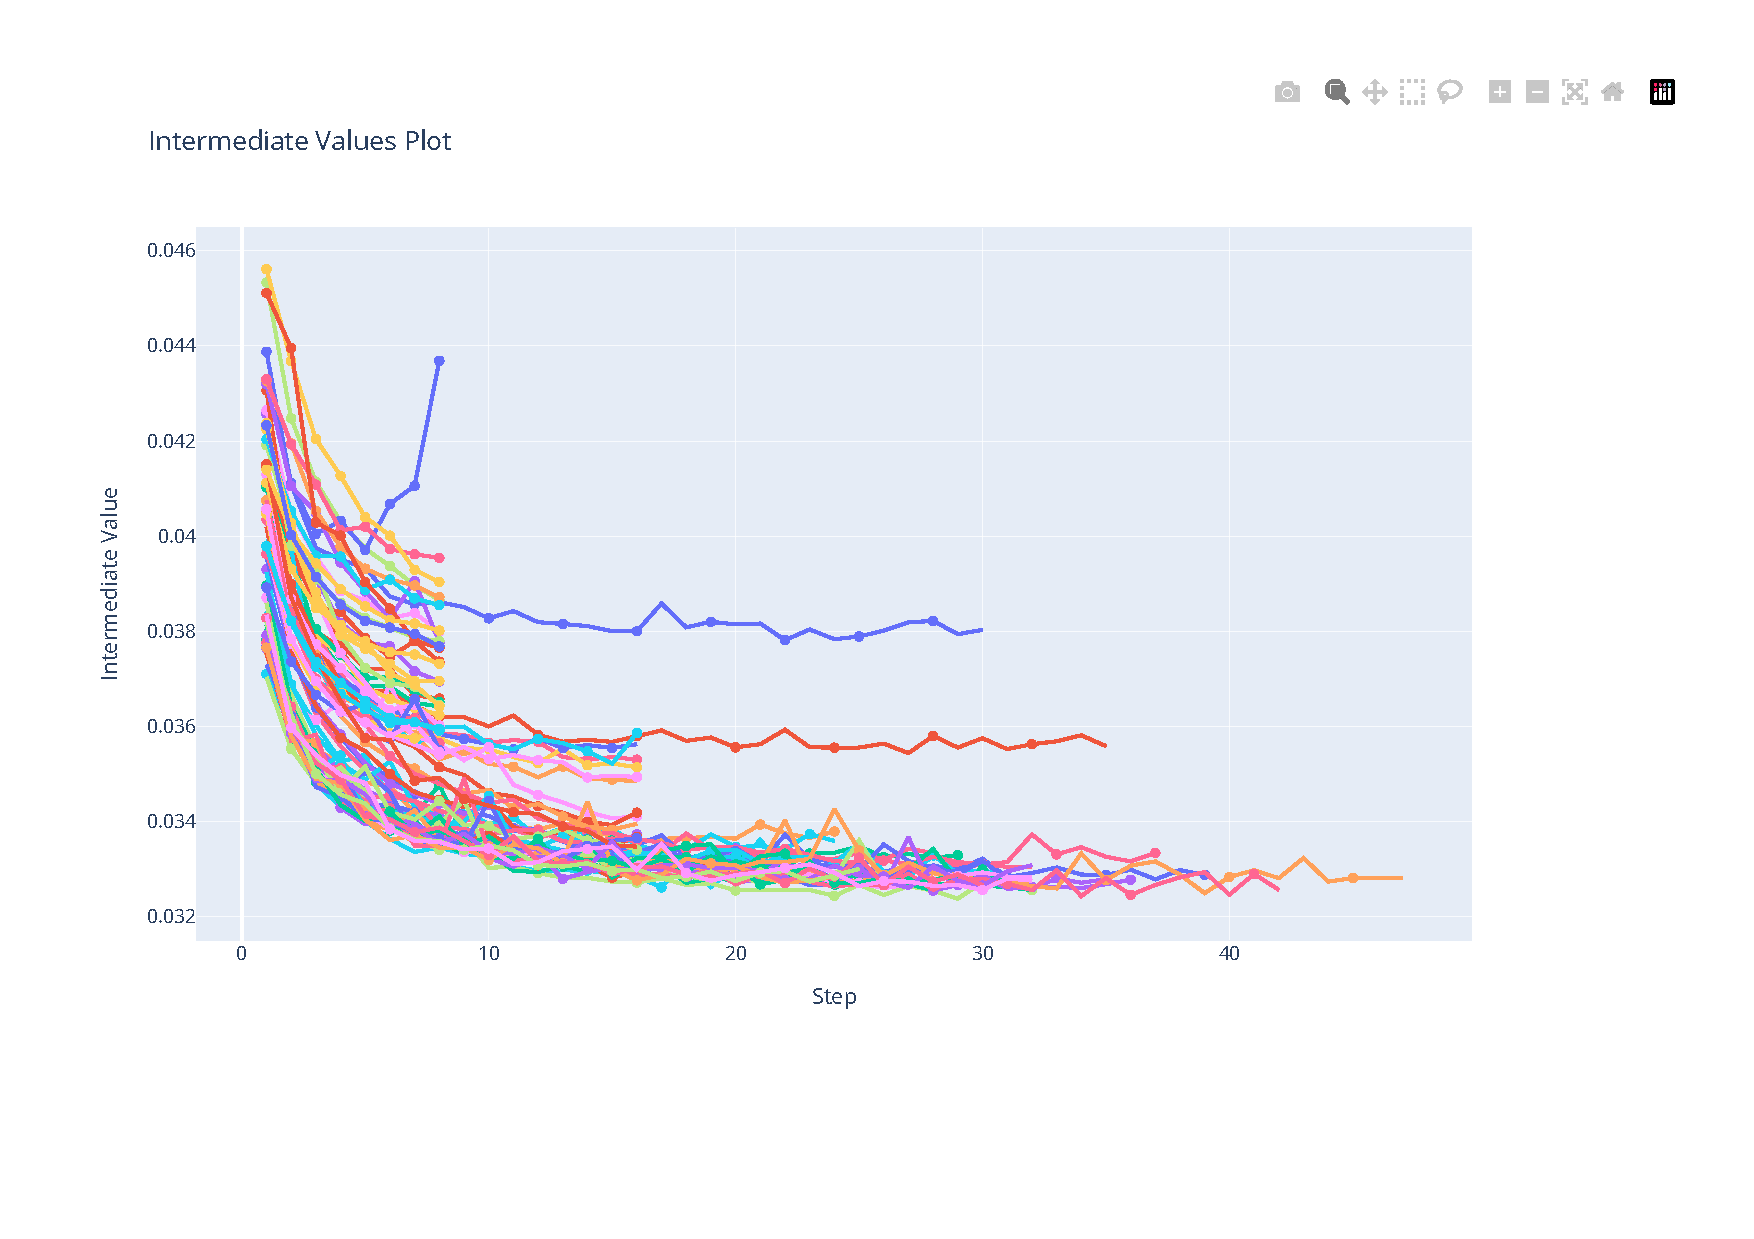
\includegraphics[width=0.9\linewidth,trim=1cm 3.5cm 5.5cm 3.5cm,clip]{figures/minimal_lstm_intermediate_values.html.pdf}
            \caption[Exp. I LSTM Intermediate Value plot]{Intermediate Value plot of \acf{LSTM} \acf{HPO} in Optuna with early stopping enabled. Successive Halving was applied to all trials, except the initial 16. The Drop-offs at stept 8, 16 and 32 indicate points, where the current batch was evaluated and the bottom-performing configurations were terminated}
            \label{fig:succhalfing}
        \end{figure}
        The best-found configuration was retrained from scratch on the full
        training set for up to \texttt{max\_epochs} epochs using the same
        early-stopping criterion, and the resulting checkpoint was used for final
        evaluation on the test split.
        It should be noted that parameter importance scores derived from a pruned
        study are biased towards values that are important early on in the convergence, rather than final validation loss, since most trials do not run to full completion.
         
         Optuna keeps track of intermediate results, enabling us to analyse the learning dynamics after an optimisation run.
          A complete specification of the hyperparameter optimisation methodology and configurations for all experiments is detailed in Table ~\ref{tab:hpo-config} in Appendix \ref{appx:B}.
          Furthermore, the corresponding hyperparameter search spaces for each model are defined within the respective methodology sections (Sections \ref{sec:method-cv} to \ref{sec:method-lstm}) and are additionally summarised in Table \ref{tab:model_hyperparameters} in Appendix \ref{appx:B}.



                
        \paragraph{Search Spaces and Strategies.}
        The optimisation strategy varies according to the complexity of the model:
        \begin{itemize}
            \item \textbf{Kinematic Models:} These models contain small, 1-Dimensional search spaces. We employed a full grid search over all valid configurations to ensure the global optimum for these parameters was found.  \ac{TPE} with n trials $\gg$ valid configurations can also find the global optimum, but comes with a computational overhead we wanted to avoid. For fairness, we only used the validation split for this optimisation, ignoring the test split.
            \item \textbf{Filters:} We mapped the Covariance and Uncertainty matrices to a multi-dimensional continuous search space using log-uniform distributions, as the optimal values typically span several orders of magnitude. The search was then guided using \ac{TPE}.
            \item \textbf{Foundation Models:} Chronos is designed as a pure Zero-Shot model and requires no \ac{HPO}. For TiREX, we optimised the size of the input window analogously to the kinematic models, since the model does not implement any attention mechanisms.
            \item \textbf{Learned Sequence Models:} These models involve higher-dimensional parameter spaces. We used \acs{TPE} to navigate the search space.

        \end{itemize}
            
           \paragraph{Feature Selection.} 
           \label{subsub:featureselection}
        
           Within the optimisation process of our models, we treated the input feature subset as a categorical hyperparameter. Rather than relying on manual feature ablation, the selection of which \ac{AIS} signals to include is then integrated directly into the search space. This reflects prior research showing that optimal feature subsets and model hyperparameters are interdependent, as the best configuration for one inherently depends on the other \parencite{Feurer2015}.
           The automated selection was not used for univariate models (TiREX), where other channels cannot influence performance, and models that implement attention across channels (Chronos-2), since those already autonomously identify the most relevant contributions during training and make explicit feature search redundant.                 
           %Absolute $x,y$ positions are strictly excluded from the search space of the deep-learning models to force them to learn generalizable vessel dynamics rather than location-specific patterns. \me{zum dritten.. am ende schauen was wo steht und dann halt nur das erste behalten}
        To make sure that all 16 candidate feature sets were covered at least once in model training of the \acs{LSTM}, one trial was enqueued to the study for each candidate. Those trials were identical, except for the feature set. After that, 10 additional startup trials were sampled uniformly at random %to seed the surrogate        model 
        before the optimisation began. The full search space for the \acp{LSTM} is listed
        in Table~\ref{tab:lstm-hpo}. 


        
                          
     \begin{table}[t]
        
        \centering
        \begin{tabular}{lll}
        \toprule
        \textbf{Hyperparameter} & \textbf{Type} & \textbf{Values / Range} \\
        \midrule
        \texttt{hidden\_size}   & Categorical & $\{64, 128, 256\}$ \\
        \texttt{num\_layers}    & Fixed       & $2$ \\
        \texttt{dropout}        & Continuous  & $[0.1,\, 0.4]$ (uniform) \\
        \texttt{learning\_rate} & Continuous  & $[10^{-4},\, 10^{-2}]$ (log-uniform) \\
        \texttt{batch\_size}    & Categorical & $\{128, 256, 512\}$ \\
        %\texttt{feature\_set}   & Categorical & $\{dx\_norm, dy\_norm\} \cup \mathcal{P}\big(\{ \{cog\_sin\_norm, cog\_cos\_norm\}, sog\_norm, rot\_norm \}\big)$ \\
        \texttt{feature\_set} & Categorical & %$\{dx\_norm, dy\_norm \cup S \}$ \\
        $\{\texttt{dx\_norm},\, \texttt{dy\_norm}\} \cup S$ \\
        \bottomrule
        \end{tabular}
        \\ with $S \in \mathcal{P}(\{\{cog\_sin\_norm, cog\_cos\_norm\}, sog\_norm, rot\_norm, dt\_norm\})$
        \caption[LSTM Hyperparameter Search Space]{Hyperparameter search space used for the \ac{LSTM} model optimization. Continuous parameters are sampled from uniform or log-uniform distributions, categorical parameters are selected from predefined sets. For the \texttt{feature\_set}, The base input always includes $\texttt{dx\_norm, dy\_norm}$. The remaining features are drawn from the power set $\mathcal{P}$ of $\{\{\texttt{cog\_sin\_norm}, \texttt{cog\_cos\_norm}\}, \texttt{sog\_norm}, \texttt{rot\_norm}, \texttt{dt\_norm}\}$, where sine and cosine of \acf{COG} are treated as an indivisible pair 
        \me{We always take dx and dy as an input. for all other inputs, we take all possible combinations of these, with the restriction of sine and cosine of cog only appearing together. since power sets are not applied recursively, this notation seems complicated, but is unambiguous. or did i make a mistake?}}
        \label{tab:lstm-hpo}

        \end{table}   
        


\section{Implementation Details}
\label{sec:impldetails}
\me{i moved this full section into the experimental setup. all general information is included in the methdos section}

    %\subsection{Sequence Model Implementation}%the ones i chose in chapter 2 
    \label{sec:sequenceimplementation}
    In this section, we describe the sequence models we have selected for vessel trajectory prediction and how they were implemented. Two categories were evaluated: foundation models applied zero-shot, and \ac{LSTM} models trained on the full dataset.      
        \subsection{Foundation Models} %some points double with the Framwwork chapter, but i feel like they belong in both. e.g. the zero shot evaluation and hpo. here it i smore detailed
        \paragraph{TiRex.}
        \textcite{auer2025tirexzeroshotforecastinglongtrex} designed TiRex as a Univariate Zero-Shot Forecaster that leverages the new scaling capabilities of the \ac{x-LSTM}.
        Our implementation is characterised by:
        \begin{enumerate}
            \item Univariate channels: To predict $dx, dy$, we fed the model only with the normalised $dx\_norm$, $dy\_norm$, which the model treats independently.
            \item Zero-Shot Evaluation: We used the Model as is. Because no attention mechanisms is implemented, we optimised only the input length. Due to the univariate character, feature selection was not a factor in our optimisation.
            %\item Probabilistic Modelling: TiRex generates quantile forecasts for the prediction horizon. %In this implementation, we use the quantiles 0.1 and 0.9.  to evaluate uncertainty via interval width, coverage,  and Winkler score. % \me{nur auf nachfrage näher drauf eingehen, denke das kennt man} \
            %\me{move evaluation} \todo!
        \end{enumerate}
        

        
        \paragraph{Chronos-2.}
         
        % https://proceedings.mlr.press/v162/ozturk22a/ozturk22a.pdf ) for weights no HPO
        In addition to the univariate TiRex, we implemented Chronos-2 \parencite{ansari2025chronos2} as a zero shot transformer for time series forecasting. Unlike the \ac{LSTM} based model, it lacks the inductive bias for time series. Instead, it supports Co-variate informed forecasting.  %\\%unrelated
        The model was designed to estimate a probability distribution over future trajectories rather than computing a deterministic path. Our implementation is characterised by:
    
        \begin{enumerate}
            \item Multivariate Covariates: To predict $dx, dy$, we fed the model with all available normalised features: $sog\_norm$, $cog\_sin\_norm$, $cog\_cos\_norm$, $dt\_norm$, $rot\_norm$  as covariates, in addition to the $dx\_norm$, $dy\_norm$ channels.
            \item Zero-Shot Evaluation: We used the Model as is, without doing any \ac{HPO} or finetuning. To avoid overhead, we deliberately did not add the feature selection to our \ac{HPO}, since we can assume, that the cross-channel attention of Chronos-2 already gives low weights to irrelevant features. %\me{siehe comments}%\ref{fig:platzhalter_test_channel_importance_chronos2_zero_shot.png} assumption bestätigen in auswertung \cite{someone to undermine this is good methodology}. 
            For a similar reason, the context length was set to the maximum 10 steps available after preprocessing, as the self attention implemented in the transformer can recognise irrelevant timestamps. %\ref{figplatzhalter_ gleichemitzeit}
            %\item Probabilistic Modelling: Chronos-2 generates quantile forecasts for the prediction horizon. In this implementation, we use the quantiles 0.1, 0.5, and 0.9. The median $q_{0.5}$ is used as the point forecast. The remaining quantiles are used to evaluate uncertainty via interval width, coverage, % CRPS approximation, and Winkler score. % \me{nur auf nachfrage näher drauf eingehen, denke das kennt man}
        \end{enumerate}
    
    
        \begin{comment}

        Beyond our standard metrics, we compute the%two scores post-hoc:
        %\textbf{Channel Importance}. This analysis ranks the predictive information of input features. For each covariate, the Pearson correlation between the feature values and the vessel's movement is computed. The resulting absolute correlations are normalised to provide a relative importance score for each input channel.
        \textbf{Channel Importance}. This analysis quantifies the linear association between each input feature and the vessel's motion magnitude. For each covariate, the absolute Pearson correlation with the motion magnitude is computed across all samples, then normalised by the sum of all absolute correlations to yield a relative importance score for each input channel.
        \textbf{Timestep Importance}. This analysis quantifies the linear association between each context timestep's motion magnitude and the future motion score. For each timestep in the context window, the absolute Pearson correlation with the future motion score is computed across all tracks, then normalised by the sum of all absolute correlations to yield a relative importance score per timestep. If all correlations are zero, uniform weights are assigned.
                
        \textbf{Timestep Importance}. This analysis quantifies the model’s temporal sensitivity. It computes the correlation between the movement at each context step and the future motion. The resulting scores reveal the model's "attention" distribution.
        \me{please tell me if this makes sense, the plots show nearly no difference except for lock, which might make sense}
        \me{scrapped, still in the code though. Actually results make sense becuse ofr lock its differnt as we are standing first. but metric was too ambigious and hard to explain}


        weggelassen weil: 
        The importance is computed from the correlation between input covariates and motion magnitude in the data  not from anything the model does internally. Both Chronos and LSTM evaluate on the same tracks with the same input features, so the Pearson correlations are identical. The model is irrelevant to the calculation.

        \end{comment}


    \subsection{LSTM} %im vergleich zu den vorherigen liest sich das etwas holprig
    \label{sec:method-lstm}
  
    
    The \ac{LSTM} represents learned sequence models in our comparison.
    Unlike the kinematic models and filters, which encode an explicit motion
    assumption, the \ac{LSTM} can learn temporal dynamics directly from the data.
    Unlike the foundation models, it was trained from scratch on the \ac{AIS}
    dataset, giving full control over architecture, feature set, and training
    procedure.
    \ws{do not mention training detials here. This belongs o the experiments section.}
    
        \paragraph{Architecture.}

        The model follows a \ac{Seq2Seq} %sequence-to-sequence 
        \ws{you have this as ac} 
        encoder--decoder design
        (Figure~\ref{fig:mylstm}): a stacked \ac{LSTM} encoder
        processes the context window and compresses it into a hidden state, which
        seeds the decoder. The decoder then predicts all future displacements simultaneously. We picked the linear prediction instead of an autoregressive decoder, due to the faster compute time.
        \ws{These are all experiment-related details, not method-sepcific.        Example, instead of writing how many layers you picked in the experiments, here you can write about the LSTM AE can have multiple stacked layers in general.} 
        % and its better suitability for short prediction horizons \me{source}.
        
        %an autoregressive decoder. \todo{design decision} The decoder predicts one displacement
        %step $(\hat{\Delta x}, \hat{\Delta y})$ at a time, feeding each prediction
        %back as the next input for up to $T_p$ steps.
        
        %The absolute trajectory is then reconstructed by cumulative summation of the displacements, offset by the last known position, as described in Section~\ref{sec:evaluation-framework}.
        The number of layers was fixed at 2 to keep the search space reasonable. Dropout was applied between layers for regularisation. More more details about the feature selection can be found in Section \ref{subsub:featureselection}. 
        \begin{figure} [h]
            \centering
            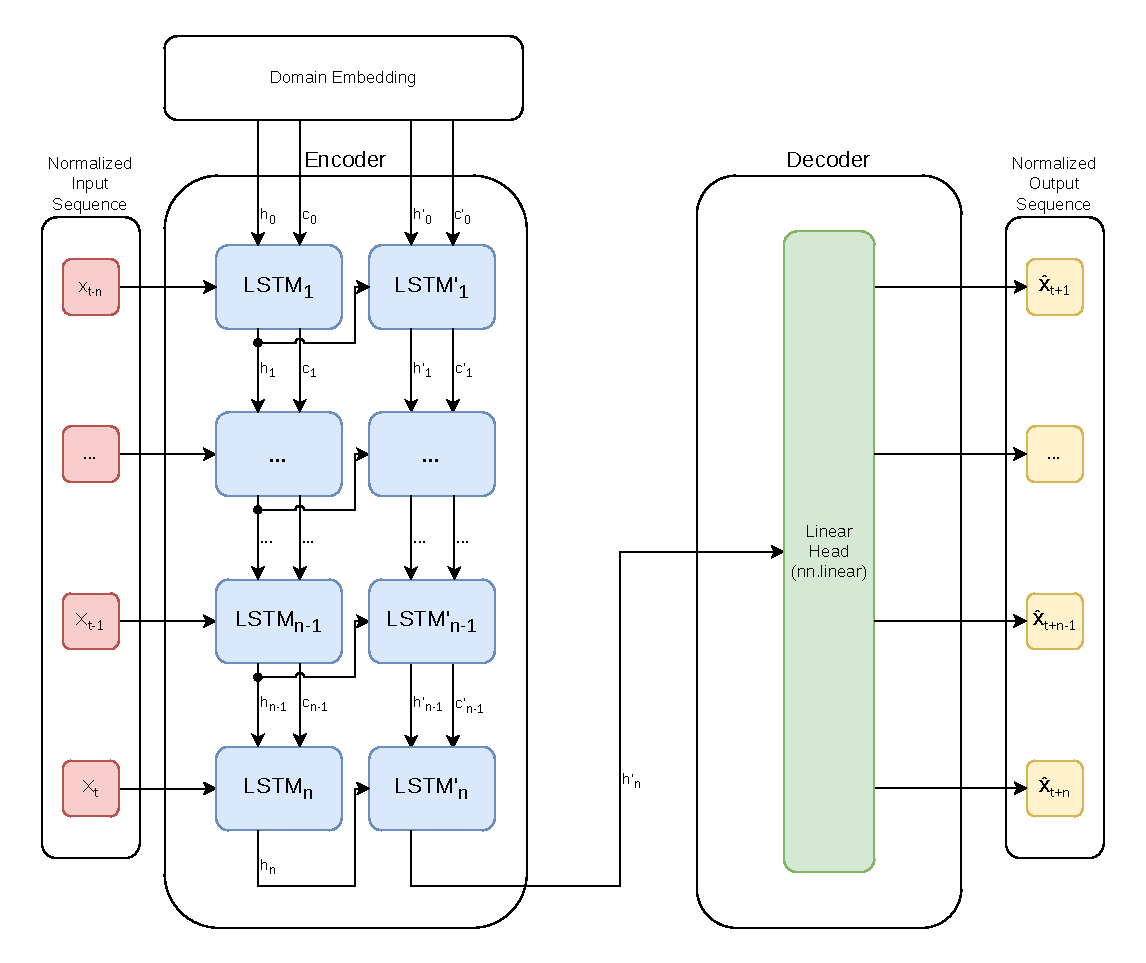
\includegraphics[width=0.85\linewidth]{figures/MyLSTM.drawio.pdf}
            \caption[Proposed LSTM Architecture]{The \acf{LSTM} Architecture implemented in this work: 2 \ac{LSTM} Encoding Layers feed into a Linear Decoder. The Initial Cell and Hidden state are initialised with the Embedded Domain. The figure is self-made.}
            \label{fig:mylstm}
        \end{figure}
        %\paragraph{Feature Selection.}
%Eigentlich alles redundant mit Evaluation Framework
        %\me{unsure if the followiong 2 sentences should be removed}
        \ws{Replace with: more details about the hyperparameters are in Seciton xxx}
        %As described in \ref{subsub:featureselection}, feature selection from our feature candidates is handled using categorical hyperparameters. We suggested \(sog\_norm\), \(cog\_sin\_norm\), \(cog\_cos\_norm\), \(dt\_norm\), \(rot\_norm\) as covariates, in addition to the \(dx\_norm\) and \(dy\_norm\) channels.
        
        % \(dx\_norm\), \(dy\_norm\) are always included, \(cog\_sin\_norm\), \(cog\_cos\_norm\) optionally included as a set, as well as \(sog\_norm\), \(rot\_norm\) and \(dt\_norm\)  as optional features.

        %Since this approach exploded the search space, we only ran it on a sampled 30\% of the total Training and validation set, and then continued training with the selected feature set. The optimisation picked the full feature set as the best candidate. OUTDATED
        %/home/dustin_klein/motion-models/output/08_baseline_results/runs/lstm_30_full_categorical/tuning/optuna_plots only on request

        %To make sure that every set of features is evaluated, we initially run one trial per feature set with a fixed set of hyperparameters, before further optimizing with \ac{TPE}.

        \ws{The follwing has a lot of details that is specific to you experimetns, here you only mention the methods and their implementations in general without the details specific to your experiments}
        \paragraph{Domain Encoding.}
        In the \textit{\ac{LSTM} + domain} variant, the domain is represented as a 4-dimensional one-hot encoded vector, with one dimension per class. Instead of appending the domain vector as an input feature at every timestep, it is added to the initial hidden and cell states of both LSTM layers. Specifically, the last 4 nodes of the initial hidden state $h_0$ and cell state $c_0$ are set to the one-hot vector. The remaining nodes are initialised to zero as usual. This keeps the total hidden size identical to the baseline model and ensures a fair comparison.  %\\
        Encoding the domain only in the initial states is acceptable here, since we focus on short term predictions and only need to retain the contextual information over 10 timesteps. %\\
        We considered adding additional groupings for domains with similar expected behaviours or constraints, but decided against this in order to avoid introducing potentially incorrect assumptions about the domain structure.
       
        A learned embedding layer was considered as an alternative. However, for only four domain classes, one-hot encoding is preferable as it is parameter-free, exact, and directly interpretable. In contrast, learned embeddings introduce additional trainable parameters and reduce interpretability, since the resulting coordinates no longer correspond directly to individual domain classes. This trade-off is usually more attractive for higher-cardinality categorical variables; if the number of domains were to grow substantially in future work, an embedding-based representation could become worth it.

        
        %\paragraph{Hyperparameter Optimisation.} \me{probably also move this into the setu of experiments}

        %The hyperparameter search space for the \ac{LSTM} is summarised in Table~\ref{tab:lstm-hpo}. The optimisation methodology, including the pruning schedule and trial budget, is detailed in Section \todo{move and reference}.
    
    \begin{comment}
             Hyperparameters are tuned using \ac{TPE} via Optuna \parencite{optuna_2019}, minimising \ac{RMSE} on the validation split.
            To make sure they are all covered at least once, for each of the 16 candidate feature sets, one trial is enqueued to the study. Those trials are identical, exept for the feature set. After that, 10 additional startup trials are sampled uniformly at random %to seed the surrogate        model 
            before the optimisation begins. The full search space is listed
            in Table~\ref{tab:lstm-hpo}. 
            
                  
            
            Pruning using successive halving is applied to reduce total compute: trials are
            evaluated at fixed epoch checkpoints, where only the
            top $1/\eta$ fraction of trials ($\eta = 2$) is allowed to continue,
            while the rest are terminated early. With \texttt{min\_resource}$\,=8$
            and \texttt{min\_early\_stopping\_rate}$\,=0$, the schedule
            evaluates configurations at epochs 8, 16, 32, and 64. Within each
            surviving trial, an independent early-stopping criterion halts training if
            the validation \ac{RMSE} does not improve by more than
            \texttt{min\_delta} within a fixed patience window.
                   
            It should be noted that parameter importance scores derived from a pruned
            study are biased towards values that are important early on in the convergence, rather than final
            validation loss, since most trials do not run to full completion.
            
            The best-found configuration is retrained from scratch on the full
            training set for up to \texttt{max\_epochs} epochs using the same
            early-stopping criterion, and the resulting checkpoint is used for final
            evaluation on the test split.
    
        
   

\begin{table}[t]
        \caption[LSTM hyperparameter search space]{Hyperparameter search space used for the \ac{LSTM} model optimization. Continuous parameters are sampled from uniform or log-uniform distributions, categorical parameters are selected from predefined sets. For the \texttt{feature\_set}, the model always receives normalized positional displacements, combined with a subset $S$ drawn from the power set $\mathcal{P}$ of the remaining kinematic and temporal features: $\{\{\texttt{cog\_sin\_norm}, \texttt{cog\_cos\_norm}\}, \texttt{sog\_norm}, \texttt{rot\_norm}, \texttt{dt\_norm}\}$. \me{not sure how to explain this compactly for the table. We always take dx and dy as an input. for all other inputs, we take all possible combinations of these, with the restriction of sine and cosine of cog only appearing together}}
        \label{tab:lstm-hpo}
        \centering
        \begin{tabular}{lll}
        \toprule
        \textbf{Hyperparameter} & \textbf{Type} & \textbf{Values / Range} \\
        \midrule
        \texttt{hidden\_size}   & Categorical & $\{64, 128, 256\}$ \\
        \texttt{num\_layers}    & Fixed       & $2$ \\
        \texttt{dropout}        & Continuous  & $[0.1,\, 0.4]$ (uniform) \\
        \texttt{learning\_rate} & Continuous  & $[10^{-4},\, 10^{-2}]$ (log-uniform) \\
        \texttt{batch\_size}    & Categorical & $\{128, 256, 512\}$ \\
        %\texttt{feature\_set}   & Categorical & $\{dx\_norm, dy\_norm\} \cup \mathcal{P}\big(\{ \{cog\_sin\_norm, cog\_cos\_norm\}, sog\_norm, rot\_norm \}\big)$ \\
        \texttt{feature\_set} & Categorical & $\{\{dx\_norm, dy\_norm\} \cup S \}$ \\
        \bottomrule
        \end{tabular}
        \end{table}
        with $S \in \mathcal{P}(\{\{cog\_sin\_norm, cog\_cos\_norm\}, sog\_norm, rot\_norm, dt\_norm\})$

        \end{comment}


%%!TEX root=../main.tex
\chapter{Experiments \& Results}%todo change title to match contents
\label{chap:results}

%rough draft only
\section{Baseline vs Learned Models}
%\section{per context analysis}
%\section{ablation studies}
%\section{Error Analyzis, failure cases}



 %and evaluation
%%!TEX root=../main.tex
\chapter{Results and Evaluation}%keine interpretation
\acresetall %reset abbrevations

\label{chap:results}

\ws{No need to have a section for each experiment. You can just write the research question and answer it (The text in the current `Results` sub-section can be the answer). The Questions do not need to be subsections. Currently, there is unecessary enumeration}

\ws{The discussion can be a section where all the discussion is written instead of per-experiment}
\todo{ 
Chapter 6  needs restructuring. The content is not split in sections that has the titles of Exp 1 , 2 , 3. Not the best. It should be split by research questions then answering each followed by a discussion section.}

\sug{aim guide: Results. This section lists the results of the experiments described in the ’Experiments’
section and discusses them in detail. It also includes answers to the research questions
presented earlier in the thesis.\\IRT guide III. RESULTS
How does your method perform? Give quantitative information and illustrate with plots.
Do not give extra information on your methods in the
results section (such as method to choose parameters, or the
experimental protocol).
Give the raw facts only; do not interpret your results yet.
That means no sentences like: “The improved performance
demonstrates that the controller is effective...” or “A probable
reason for this observation is...”.
IV. DISCUSSION
Interpret your results. Is the performance acceptable? Go
back to initial questions, compare to other methods reported
in literature. How do you explain unexpected results? Which
shortcomings or limitations are there in your methods and
results? Where is room for improvement? Could combination
with methods from literature further improve the work? Mention plans, needs, and recommendations for future research.
}

\me{unsicher wie ich das angehen werde, nochmal student teacher framework vlg. da ist es aber ncht ganz wie oben beschreiben -> bischem mehr fließtext, da dann die RQ konkret stellen und beantworten. anschließend gessamlete diskussion. mache dayu neuen rewrite und behalte das hier}
\me{explicitly answer rq 2 and 3}


\section[Exp. \Romannum{1}: Motion Model Comparison]{Exp. \Romannum{1}: Baseline Comparison of Motion Models} 

This experiment serves as the overall baseline comparison across all evaluated motion models and model families on the full dataset. 
It is designed to answer \textbf{Research Question 1:} \textit{Given a preprocessed dataset, how do deep learning models, both task-specific and pretrained, kinematic baselines, and stochastic filters compare in short-term trajectory prediction of inland vessels under a systematic hyperparameter optimisation procedure?}

\subsection{Results}

The optimised hyperparameter configurations for all evaluated models are listed in Table~\ref{tab:hpo_results_exp0}, and the corresponding test set error metrics are detailed in Table~\ref{tab:results_exp0}.
To assess the overall statistical significance of these results, Figure~\ref{fig:cd_test} provides a \ac{CD} diagram based on the Friedman test and Nemenyi post-hoc comparison.
The diagram reveals a clear ranking structure: the two LSTM-based models occupy the top positions, followed by the EKF and Chronos-2, while the remaining models form a middle group with mostly non-significant pairwise differences.
The CTRV-based models rank last.

\begin{table}[t]
\centering
\caption[Exp. I Optimised hyperparameter configurations]{Optimised hyperparameter configurations for all models. Discussed metrics are shaded in.}
\label{tab:hpo_results_exp0}
\begin{tabular}{llr}
\toprule
\textbf{Model} & \textbf{Hyperparameter} & \textbf{Value} \\
\midrule
CV
  & \cellcolor{blue!15}{$n_\text{vel}$}           & \cellcolor{blue!15}{1} \\
CTRV
  & $n_\text{vel}$            & 2 \\
CTRV Arc
  & $n_\text{vel}$            & 3 \\
Hybrid CV/CTRV
  & $n_\text{vel}$ (CV)       & 1 \\
  & $n_\text{vel}$ (CTRV)     & 2 \\
  & $n_\text{rot}$            & 1 \\
  & \cellcolor{blue!15}{$\tau_\text{rot}$ }       & \cellcolor{blue!15}{29.28 °/min} \\
\midrule
KF (CV)
  & \cellcolor{cyan!15}$q_\text{pos}$ & \cellcolor{cyan!15}$1.578 \times 10^{-3}$ \\
  & $q_\text{vel}$                    & $5.932$ \\
  & \cellcolor{cyan!15}$r_\text{pos}$ & \cellcolor{cyan!15}$1.077 \times 10^{-2}$ \\
  & $p_{0,\text{pos}}$                & $7.737 \times 10^{-2}$ \\
  & $p_{0,\text{vel}}$                & $1.190 \times 10^{-1}$ \\


  EKF (CTRV)
  & \cellcolor{green!15}$q_\text{pos}$            & \cellcolor{green!15}$15.957$ \\
  & $q_\text{vel}$            & $4.290 \times 10^{-2}$ \\
  & \cellcolor{green!15}$q_\text{rot}$            & \cellcolor{green!15}$1.002 \times 10^{-7}$ \\
  & $r_\text{pos}$            & $1.792 \times 10^{-2}$ \\
  & $p_{0,\text{pos}}$        & $4.046 \times 10^{-1}$ \\
  & $p_{0,\text{vel}}$        & $1.845 \times 10^{-3}$ \\
  & $p_{0,\text{rot}}$        & $2.076 \times 10^{-6}$ \\
  & $n_\text{ctx}$            & 2 \\
\midrule
Chronos-2
  & \multicolumn{2}{l}{\textit{no HPO}} \\
TiRex
  & context length            & 1\\
\midrule
LSTM
  & hidden size               & 256 \\
  & num.\ layers              & 2 \\
  & dropout                   & 0.290 \\
  & learning rate             & $5.530 \times 10^{-4}$ \\
  & batch size                & 128 \\
  %& feature set               & no rot\\
  & \cellcolor{orange!15}feature set               & \cellcolor{orange!15}no rot\\
  \midrule
LSTM + Domain
  & hidden size               & 256 \\
  & num.\ layers              & 2 \\
  & dropout                   & 0.300 \\
  & learning rate             & $4.000 \times 10^{-4}$ \\
  & batch size                & 256 \\
  & feature set               & all\\
\bottomrule
\end{tabular}
\end{table}

\begin{table}[t]
\centering
\caption[Exp. I Test set error metrics] {Test set error metrics for all models. Discussed metrics shaded in.}
\label{tab:results_exp0}
\begin{tabular}{lrrr}
\toprule
\textbf{Model} & \textbf{ADE} & \textbf{FDE} & \textbf{RMSE} \\
\midrule
Constant Velocity   & 78.39 & 175.82 & 155.73 \\
CTRV                & 82.92 & 195.18 & 164.51 \\
CTRV Arc            & 85.21 & 196.78 & 168.29 \\
Hybrid CV/CTRV      & 78.49 & 176.45 & 155.49 \\
\midrule
KF (CV)             & 78.39 & 175.82 & 155.73 \\
EKF (CTRV)          & 78.94 & 174.88 & 151.50 \\
\midrule
Chronos-2           & 80.25 & 179.80 & 152.86 \\
TiRex               & 78.37 & 175.82 & 155.71 \\
\midrule
LSTM                & 54.78 & 121.18 & 111.36 \\
LSTM + Domain       & 53.80 & 119.02 & 109.95 \\
\bottomrule
\end{tabular}
\end{table}

\begin{figure}[h]
    \centering
    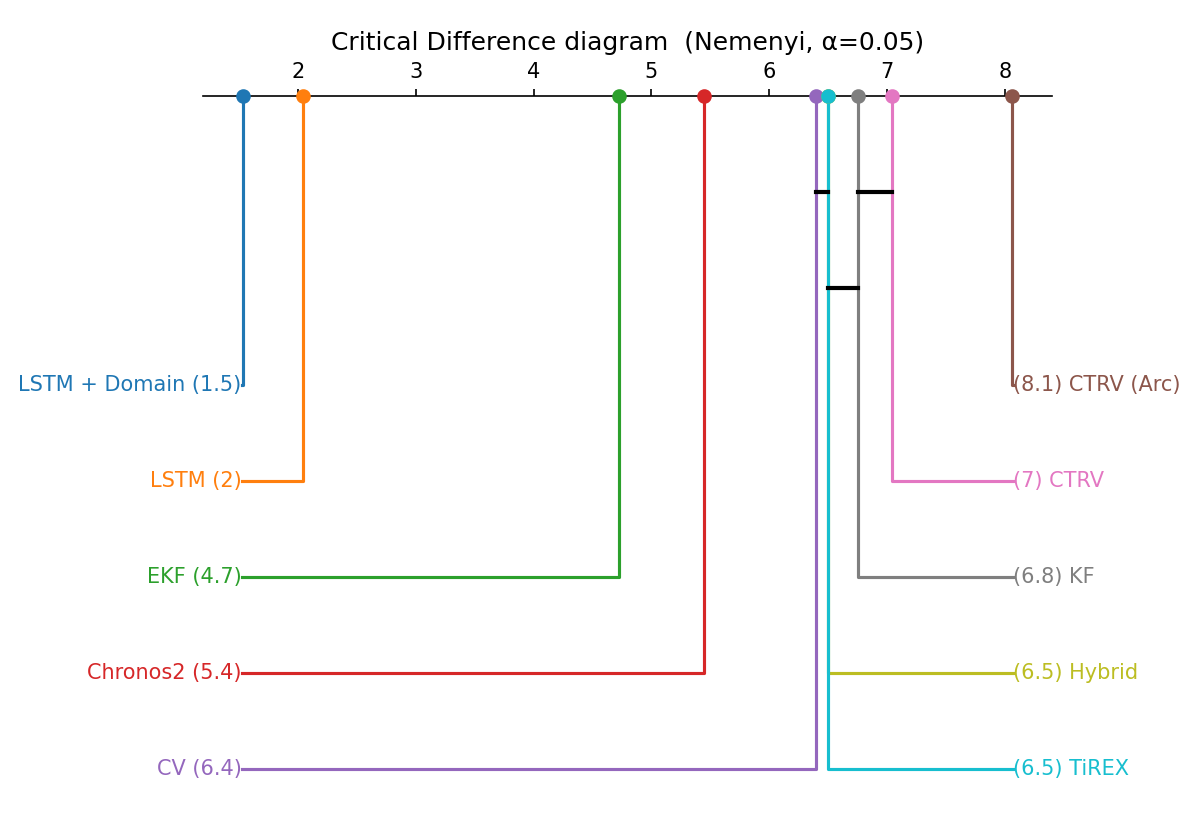
\includegraphics[width=0.7\linewidth]{figures/cd_diagram.png}
    \caption[Exp. I Friedman \& Nemenyi CD-Plot]{ \acf{CD} diagram based on the Friedman test and Nemenyi post-hoc comparison. Models connected by a horizontal bar are not significantly different at \( \alpha = 0.05\). The shown numbers are the mean rank per model in the evaluation, 1 being the best possible result.}
    \label{fig:cd_test}
\end{figure}

Figure~\ref{fig:adepredhorizon} depicts the development of the \ac{ADE} for all models over the prediction horizon. While the error for the \ac{CV} model grows approximately linearly, the errors for CTRV and CTRV Arc diverge heavily at longer horizons. The \ac{LSTM}-based models maintain the lowest \ac{ADE} across all ten prediction steps.

\begin{figure}[h]
    \centering
    \begin{tikzpicture}
    \begin{axis}[
        width=0.8\linewidth,
        height=6cm,
        xlabel={Prediction Step},
        ylabel={ADE (m)},
        xmin=1, xmax=10,
        xtick={1,2,...,10},
        ymin=0,
        grid=major,
        grid style={dashed, gray!30},
        legend style={
            at={(0.5,-0.28)},
            anchor=north,
            legend columns=4,
            font=\small
        },
        mark size=1.5pt,
        cycle list name=color list,
    ]
    
    \addplot coordinates {
        (1,7.861)(2,16.747)(3,28.983)(4,43.096)(5,60.103)
        (6,78.936)(7,100.214)(8,123.386)(9,148.728)(10,175.824)
    }; \addlegendentry{CV}
    
    \addplot coordinates {
        (1,8.353)(2,16.865)(3,28.177)(4,42.303)(5,59.811)
        (6,80.468)(7,104.477)(8,131.658)(9,161.924)(10,195.180)
    }; \addlegendentry{CTRV}
    
    \addplot coordinates {
        (1,8.976)(2,18.242)(3,30.422)(4,45.051)(5,62.918)
        (6,83.636)(7,107.548)(8,134.347)(9,164.148)(10,196.783)
    }; \addlegendentry{CTRV Arc}
    
    \addplot coordinates {
        (1,8.054)(2,16.930)(3,29.044)(4,43.019)(5,59.942)
        (6,78.772)(7,100.143)(8,123.486)(9,149.066)(10,176.446)
    }; \addlegendentry{Hybrid CV/CTRV}
    
    \addplot coordinates {
        (1,7.861)(2,16.747)(3,28.983)(4,43.096)(5,60.103)
        (6,78.936)(7,100.216)(8,123.386)(9,148.726)(10,175.824)
    }; \addlegendentry{KF (CV)}
    
    \addplot coordinates {
        (1,8.364)(2,17.853)(3,30.191)(4,44.472)(5,61.235)
        (6,79.889)(7,100.747)(8,123.511)(9,148.295)(10,174.882)
    }; \addlegendentry{EKF (CTRV)}
    
    \addplot coordinates {
        (1,8.020)(2,17.405)(3,29.932)(4,44.419)(5,61.698)
        (6,80.865)(7,102.417)(8,126.026)(9,151.936)(10,179.800)
    }; \addlegendentry{Chronos-2}
    
    \addplot coordinates {
        (1,7.860)(2,16.743)(3,28.975)(4,43.083)(5,60.084)
        (6,78.911)(7,100.189)(8,123.362)(9,148.711)(10,175.820)
    }; \addlegendentry{TiRex}
    
    \addplot coordinates {
        (1,5.769)(2,12.005)(3,20.515)(4,30.700)(5,42.527)
        (6,55.682)(7,70.279)(8,86.083)(9,103.057)(10,121.181)
    }; \addlegendentry{LSTM}

    \addplot coordinates {
        (1,5.686)(2,11.776)(3,20.143)(4,30.110)(5,41.737)
        (6,54.729)(7,69.035)(8,84.572)(9,101.244)(10,119.017)
    }; \addlegendentry{LSTM + Domain}
    
    \end{axis}
    \end{tikzpicture}
    %\caption{ADE per prediction step averaged across all tracks 
    \caption[Exp. I ADE over Time]{Progression of \acf{ADE} over time, showing the divergence of error across all ten prediction steps. The plot demonstrates that \acf{LSTM}-based architectures achieve the lowest errors, while kinematic models exhibit higher trajectory divergence, particularly as the prediction horizon increases.}
    \label{fig:adepredhorizon}
\end{figure} 

Regarding the foundation models, Table~\ref{tab:results_exp0_foundation_prob} shows the probabilistic calibration metrics.
TiRex produces extremely narrow prediction intervals (Mean Interval Width of 6.41) and achieves a coverage of only 0.059. In contrast, Chronos-2 produces wider intervals but achieves a near-ideal coverage of 0.769.
Figure~\ref{fig:violince} visualises the error distribution shapes as violin plots, showing that TiRex and the CV model share nearly identical error distributions, while the LSTM distribution is distinctly shifted toward lower errors.

\begin{table}[t]
\centering
\caption{Exp. I Probabilistic metrics for foundation models}
\label{tab:results_exp0_foundation_prob}
\begin{tabular}{lrrr}
\toprule
\textbf{Model} & \textbf{MIW} & \textbf{Coverage} & \textbf{Winkler80} \\
\midrule
Chronos-2 (zero-shot) & 145.37 & 0.769 & 114.65 \\
TiRex                 &   6.41 & 0.059 & 112.20 \\
\bottomrule
\end{tabular}
\end{table}

\begin{figure}[h]
    \centering
    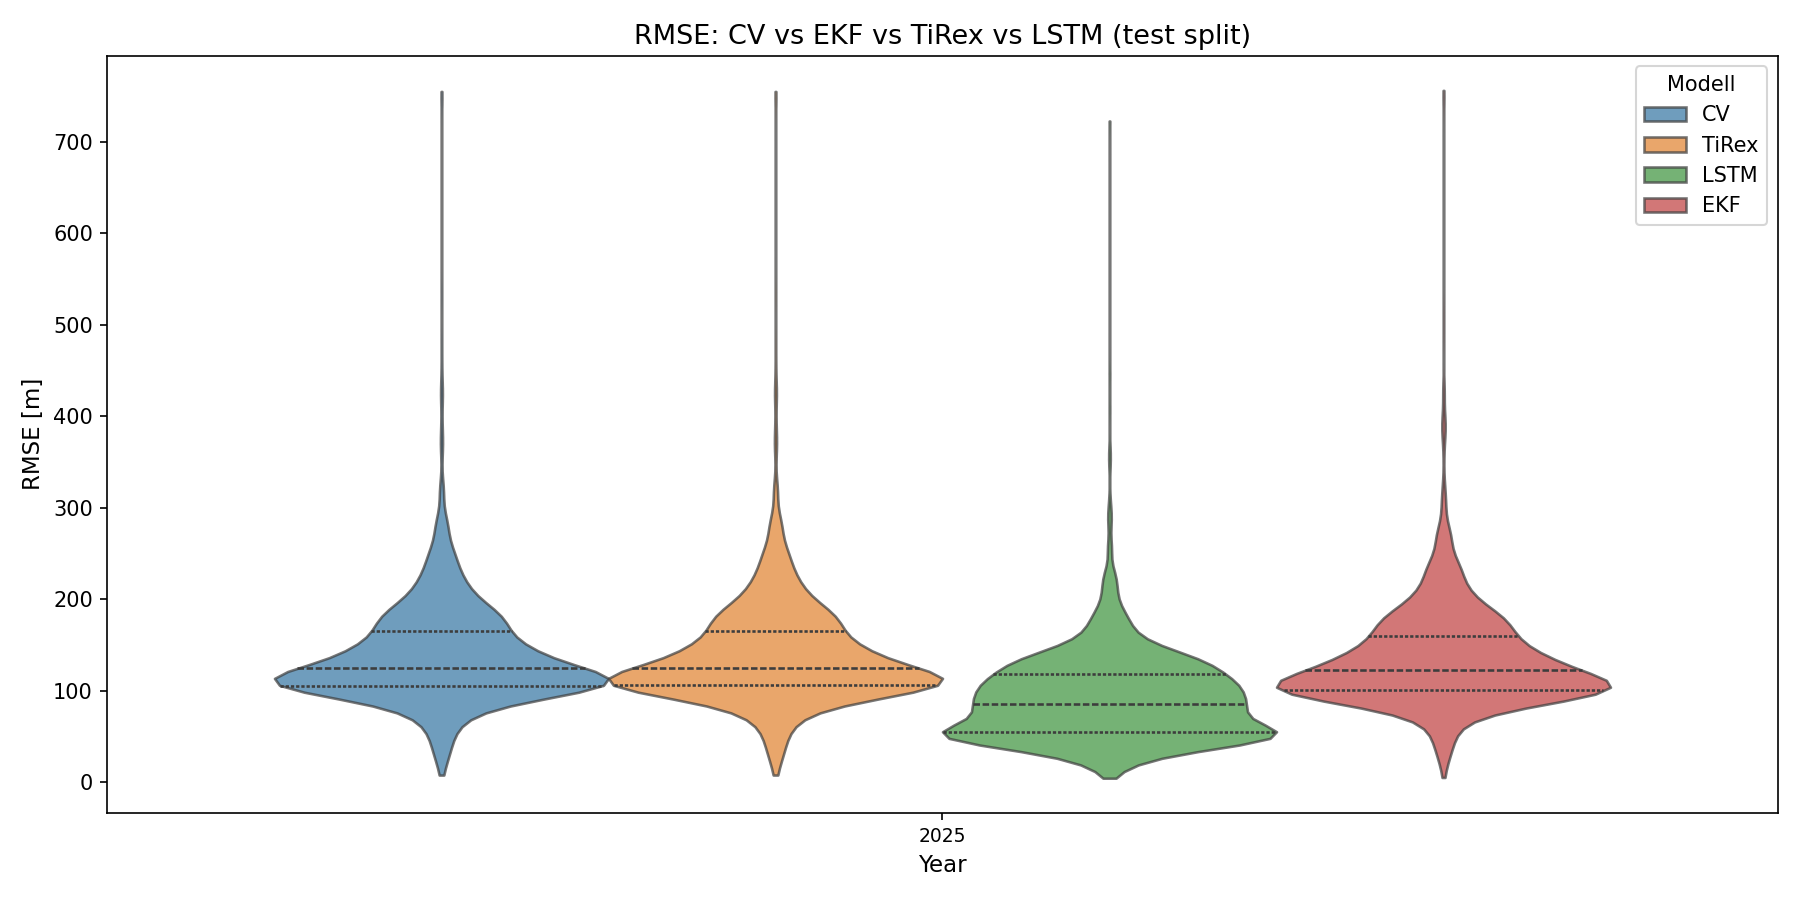
\includegraphics[width=0.98\linewidth]{test_violin_cv_ekf_tirex_lstm_per_year.png}
    %\caption{Violin Plots for CV, EKF, TiRex and LSTM}
    \caption[Exp. I RMSE Violin plots]{Violin plots visualizing the distribution of \acf{RMSE} for the \acf{CV}, \acf{EKF}, TiRex, and \acf{LSTM} models on the test set. The \ac{LSTM} model demonstrates a distinct shift toward lower error values compared to the other models , whereas the \acf{CV} and TiRex models exhibit nearly identical error distributions.}
    \label{fig:violince}
\end{figure}

Finally, the hyperparameter optimisation process for the \ac{LSTM} is visualised in Figure~\ref{fig:succhalfing} and Figure~\ref{fig:paralelcord}. Figure~\ref{fig:succhalfing} illustrates a successive halving run, demonstrating how underperforming configurations were pruned early.
Figure~\ref{fig:paralelcord} presents a parallel coordinate plot of the parameter search. It reveals a clear band around the optimal configuration and indicates that the model selected a feature set that explicitly excluded the \ac{ROT}).
Furthermore, Figure~\ref{fig:monthlytrends-all} plots the average \ac{RMSE} per month over the full dataset, with consistent performance trends across all models.

\begin{figure}[h]
    \centering
    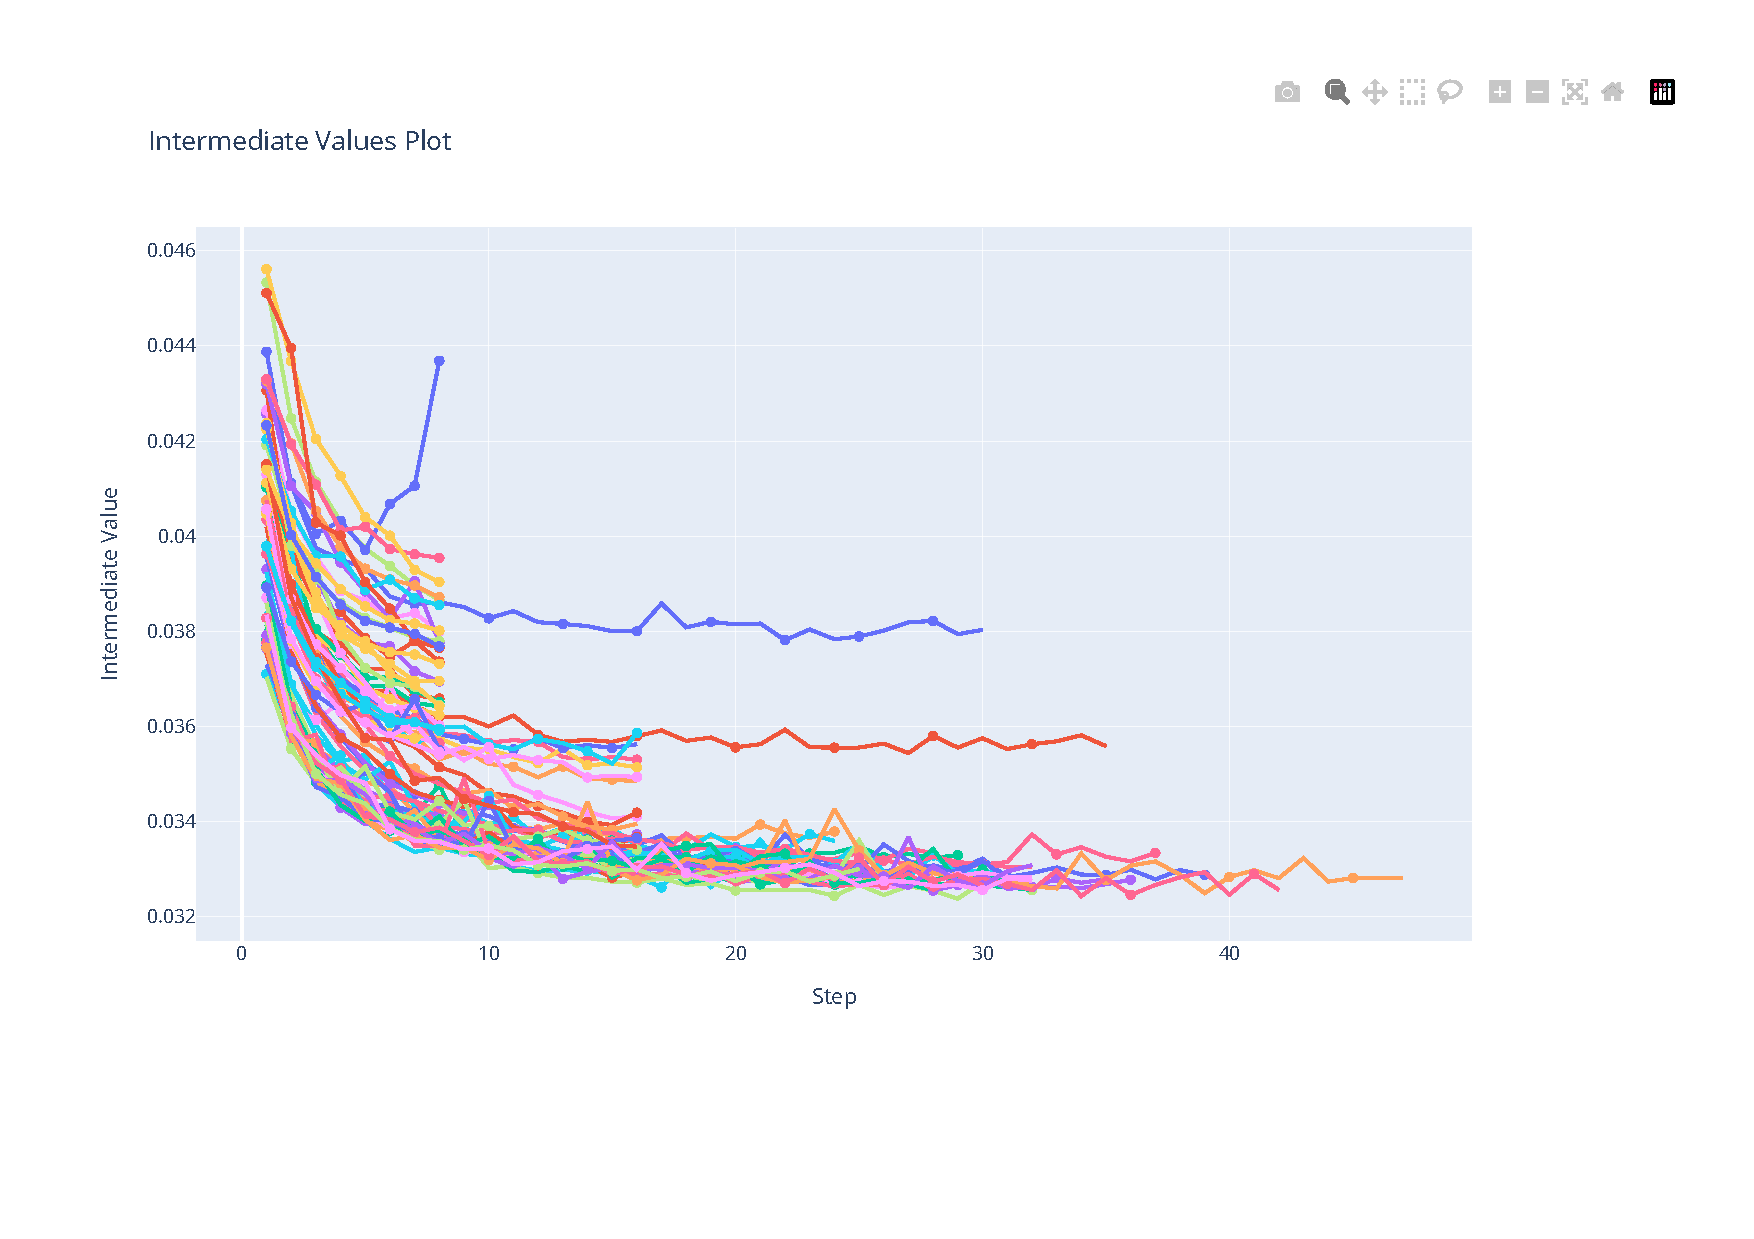
\includegraphics[width=0.95\linewidth,trim=1cm 3.5cm 5.5cm 3.5cm,clip]{figures/minimal_lstm_intermediate_values.html.pdf}
    \caption[Exp. I LSTM Intermediate Value plot]{Intermediate Value plot of \acf{LSTM} \acf{HPO} in Optuna with early stopping enabled. Successive Halving was applied to all trials, except the initial 16.}
    \label{fig:succhalfing}
\end{figure}

\begin{figure}[h]
    \centering
    %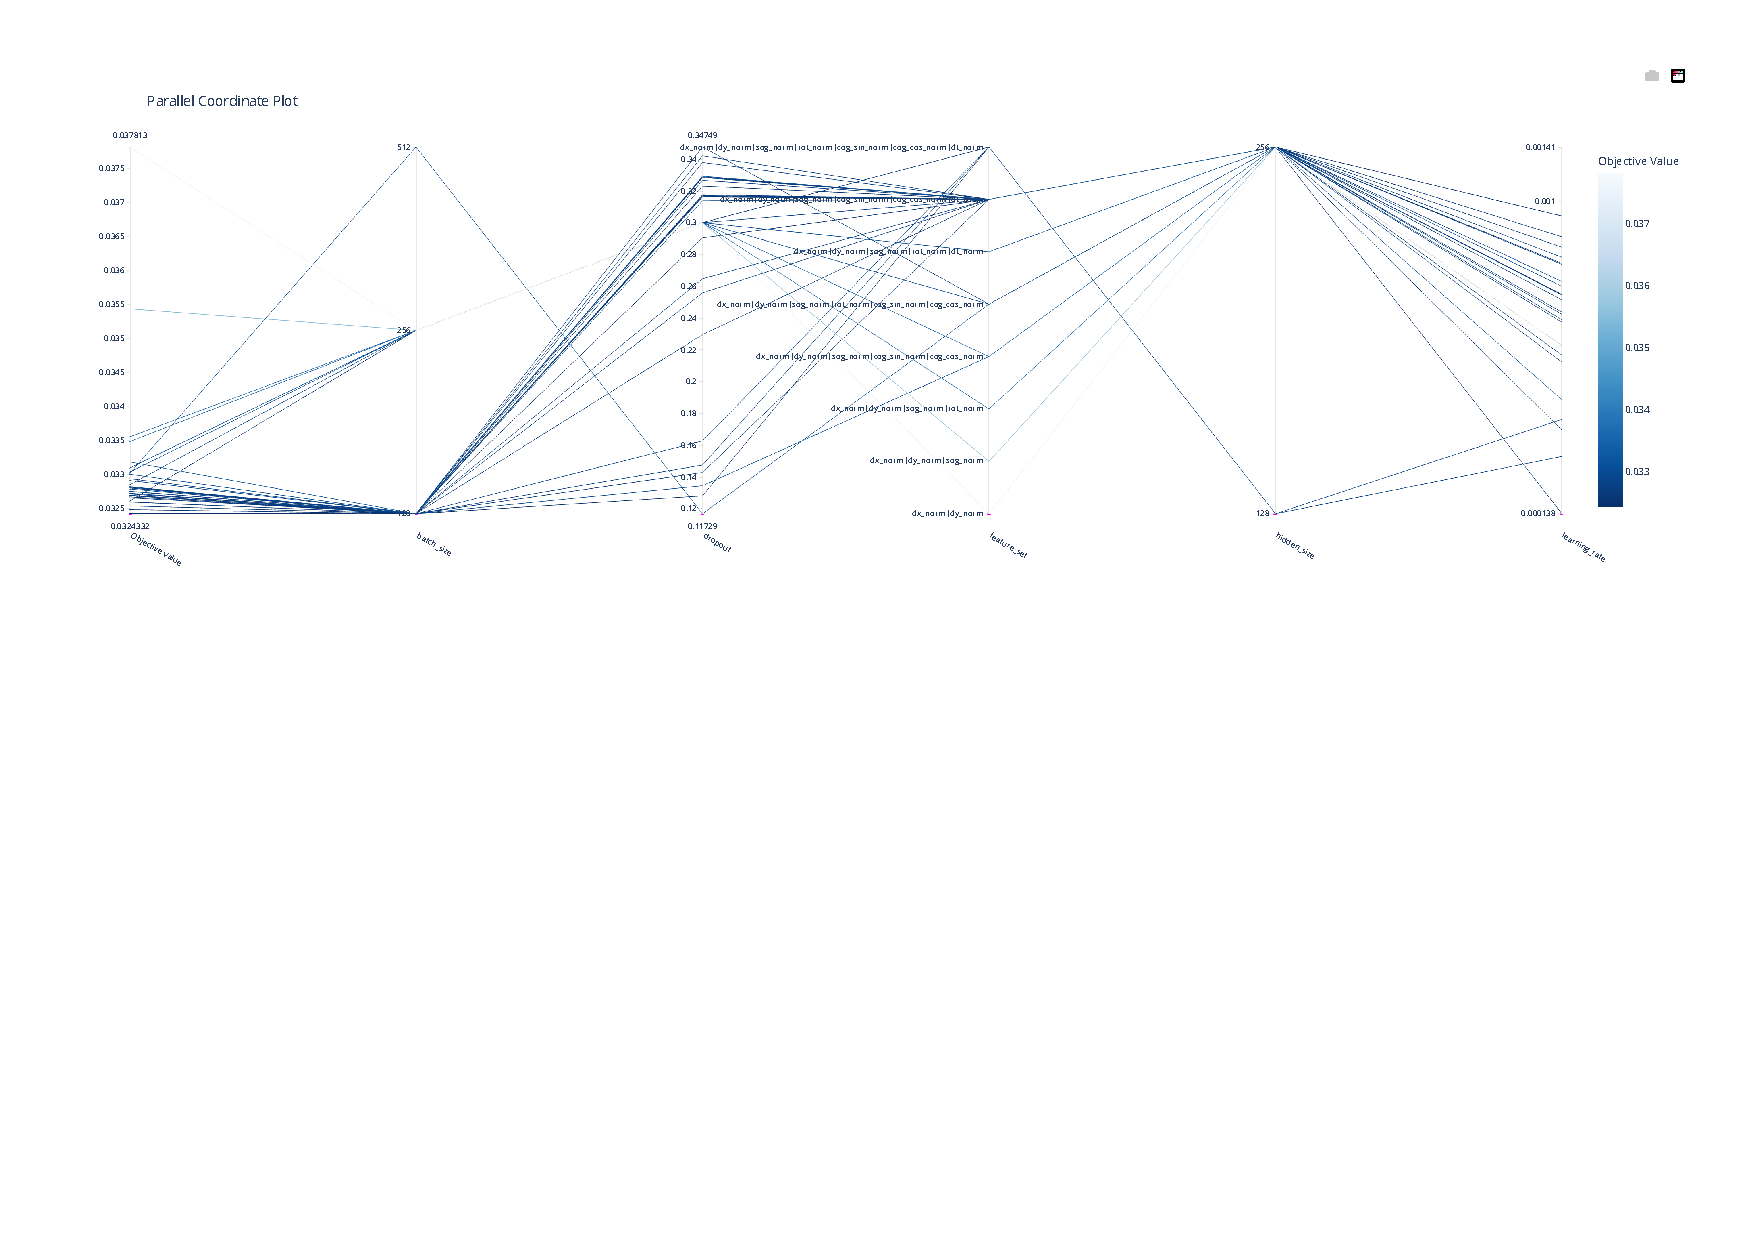
\includegraphics[width=1\linewidth,trim=1cm 10.5cm 1cm 1.5cm,clip]{figures/minimal_lstm_parallel_coordinate.html.pdf}
    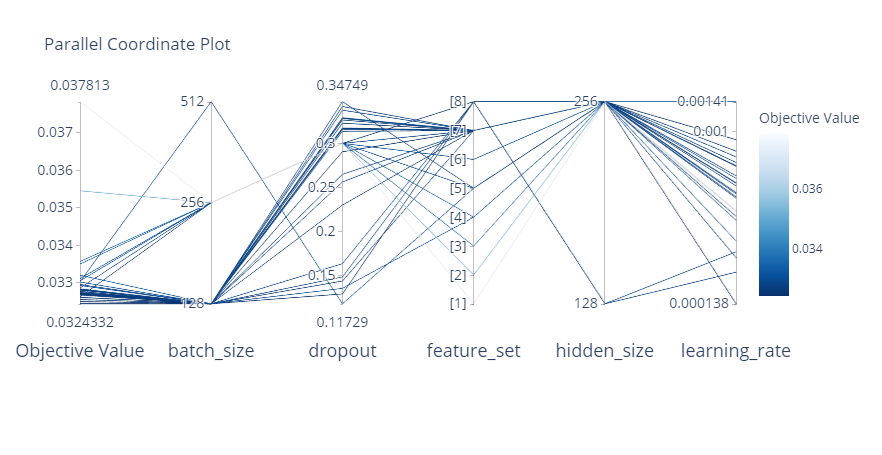
\includegraphics[width=1\linewidth, trim=0cm 3.1cm 0cm 2cm,clip]{figures/paralelcoord_zoomed.png}
    %\caption[Exp. I LSTM Parallel Coordinate Plot]{Parallel Coordinate Plot of \acf{LSTM} Hyperparameter selection, showing a clear band around the selected hyperparameter configuration. \todo{add 1, 2, 3...}}
    \caption[Exp. I LSTM Parallel Coordinate Plot]{Parallel Coordinate Plot of \acf{LSTM} Hyperparameter selection, showing a clear band around the selected hyperparameter configuration. Feature set mappings: [1] dx\_norm, dy\_norm; [2] dx\_norm, dy\_norm, sog\_norm; [3] dx\_norm, dy\_norm, sog\_norm, rot\_norm; [4] dx\_norm, dy\_norm, sog\_norm, cog\_sin\_norm, cog\_cos\_norm; [5] dx\_norm, dy\_norm, sog\_norm, rot\_norm, cog\_sin\_norm, cog\_cos\_norm; [6] dx\_norm, dy\_norm, sog\_norm, rot\_norm, dt\_norm; [7] dx\_norm, dy\_norm, sog\_norm, cog\_sin\_norm, cog\_cos\_norm, dt\_norm; [8] dx\_norm, dy\_norm, sog\_norm, rot\_norm, cog\_sin\_norm, cog\_cos\_norm, dt\_norm.} \me{new version with increased font sizes and feature sets not witten explcicitly}
    \label{fig:paralelcord}
\end{figure}


\begin{figure}[h]
    \centering
    \begin{tikzpicture}
    \begin{axis}[
        name=main,
        width=0.85\linewidth,
        height=8cm, 
        xlabel={Month},
        ylabel={RMSE (m)},
        ymin=75, ymax=175, 
        xmin=0.5, xmax=12.5,
        xtick={1,2,...,12},
        xticklabels={Jan,Feb,Mar,Apr,May,Jun,Jul,Aug,Sep,Oct,Nov,Dec},
        xticklabel style={rotate=45, anchor=east, font=\small},
        grid=major,
        grid style={dashed, gray!30},
        legend style={
            at={(0.5,-0.38)},
            anchor=north,
            legend columns=4,
            font=\small
        },
        mark size=1.5pt,
        cycle list name=color list,
        axis y line*=left,
        axis x line*=bottom,
    ]
    
    \addplot coordinates {
        (1,150.68)(2,146.54)(3,145.76)(4,148.09)(5,134.58)
        (6,130.30)(7,127.56)(8,133.85)(9,133.55)(10,143.01)
        (11,134.22)(12,134.11)
    }; \addlegendentry{CV}
    
    \addplot coordinates {
        (1,154.44)(2,150.62)(3,151.49)(4,153.95)(5,138.43)
        (6,135.97)(7,133.14)(8,138.42)(9,137.73)(10,149.36)
        (11,139.39)(12,136.40)
    }; \addlegendentry{CTRV}
    
    \addplot coordinates {
        (1,160.16)(2,155.51)(3,156.69)(4,159.50)(5,142.50)
        (6,139.55)(7,136.44)(8,142.23)(9,142.46)(10,153.20)
        (11,143.27)(12,141.02)
    }; \addlegendentry{CTRV Arc}
    
    \addplot coordinates {
        (1,151.39)(2,147.01)(3,146.20)(4,147.73)(5,134.67)
        (6,131.39)(7,127.38)(8,134.15)(9,134.07)(10,143.37)
        (11,133.93)(12,133.65)
    }; \addlegendentry{Hybrid CV/CTRV}
    
    \addplot coordinates {
        (1,150.68)(2,146.54)(3,145.76)(4,148.09)(5,134.58)
        (6,130.30)(7,127.56)(8,133.85)(9,133.55)(10,143.01)
        (11,134.22)(12,134.11)
    }; \addlegendentry{KF (CV)}
    
    \addplot coordinates {
        (1,146.42)(2,142.48)(3,141.74)(4,144.76)(5,130.69)
        (6,126.45)(7,124.73)(8,130.01)(9,130.24)(10,139.55)
        (11,130.87)(12,130.29)
    }; \addlegendentry{EKF (CTRV)}
    
    \addplot coordinates {
        (1,146.06)(2,143.09)(3,141.57)(4,143.28)(5,130.72)
        (6,124.68)(7,126.37)(8,129.56)(9,132.99)(10,140.82)
        (11,131.24)(12,130.51)
    }; \addlegendentry{Chronos-2}
    
    \addplot coordinates {
        (1,150.65)(2,146.52)(3,145.73)(4,148.08)(5,134.58)
        (6,130.29)(7,127.55)(8,133.85)(9,133.54)(10,143.00)
        (11,134.21)(12,134.09)
    }; \addlegendentry{TiRex}
    
    \addplot coordinates {
        (1,98.00)(2,93.24)(3,96.86)(4,93.53)(5,90.71)
        (6,83.01)(7,87.67)(8,89.58)(9,90.85)(10,97.84)
        (11,87.86)(12,90.82)
    }; \addlegendentry{LSTM}

    \addplot coordinates {
        (1,90.84)(2,86.57)(3,93.25)(4,91.92)(5,85.43)
        (6,79.95)(7,83.18)(8,85.01)(9,86.97)(10,92.49)
        (11,83.83)(12,86.24)
    }; \addlegendentry{LSTM + Domain}
    
    \end{axis}
    
    \begin{axis}[
        width=0.85\linewidth,
        height=8cm,
        ymin=0, ymax=160000,
        xmin=0.5, xmax=12.5,
        xtick=\empty,
        ylabel={$n_\text{tracks}$},
        ylabel style={at={(1.08,0.5)}, color=violet},
        ytick={0,40000,80000,120000},
        yticklabels={0,40k,80k,120k},
        yticklabel style={font=\small, color=violet},
        ytick style={color=cyan},
        axis y line*=right,
        axis x line=none,
        bar width=0.55,
    ]
    
    \addplot[ybar, fill=violet, draw=none, fill opacity=0.25] coordinates {
        (1,73177)(2,61903)(3,75120)(4,71784)(5,83023)
        (6,82636)(7,93205)(8,106326)(9,86547)(10,71582)
        (11,64072)(12,53443)
    };
    
    \end{axis}
    \end{tikzpicture}
    %\caption{RMSE per month with track count shown as violet bars\todo{from here on, expand figure and table captions}}
    \caption[Exp. I RMSE monthly trends]{Comparison of \acf{RMSE} by month, demonstrating consistent performance trends across all models. Violet bars indicate the monthly volume of tracks}
    \label{fig:monthlytrends-all}
\end{figure}

\FloatBarrier %\me{leave this up?}

\subsection{Discussion}

The results provide a clear answer to the first research question: learned sequence models, particularly task-specific \acp{LSTM}, significantly outperform both classical kinematic models and stochastic filters in predicting short-term inland vessel trajectories. 

\paragraph{Kinematic Models.}
The performance of the kinematic models suggests that simple arc estimations are insufficient to outperform straight-line motion prediction. The \ac{CV} model learned to only use the velocity of the most recent timestep (highlighted in purple in Table~\ref{tab:hpo_results_exp0}).
This is an assumption that is also applied in most \ac{CV} definitions, which was relaxed for these experiments. With increasing model complexity, the best context size increases. The Hybrid Model learns to switch to \ac{CV} at a relatively small $\tau_\text{rot}$ of $29.28^\circ/\text{min}$. This indicates that straight-line motion is more prevalent than motion with a single arc in our dataset. 

Furthermore, Figure~\ref{fig:adepredhorizon} shows the error progression over time. While the \ac{ADE} of the \ac{CV} model does not grow perfectly linearly, it has a much more linear trend compared to the \ac{CTRV} models, which diverge heavily at longer horizons.
One cause for this difference is that the deviation of a circular arc generated by an unsuitable turn rate in \ac{CTRV} grows superlinearly with the number of prediction steps. In contrast, a wrong velocity estimate in \ac{CV} produces a constant lateral offset that accumulates linearly. This dynamic can be visually grasped by looking at the upper rows of Figures~\ref{fig:domain1} and \ref{fig:domain3}.


\paragraph{Stochastic Filters.}

The \ac{KF} does not outperform the \ac{CV} model. Since the \ac{CV} model learned to only look at the last step, the Markov assumption of the \ac{KF} does not introduce any additional drawbacks. In the \ac{KF}, position changes are a linear function of the velocity state, so positional errors remain small as long as the velocity estimate is reasonable.
Consequently, the optimization selected a relatively small process noise $q_\text{pos}$ compared to the measurement noise $r_\text{pos}$ (highlighted in cyan in Table~\ref{tab:hpo_results_exp0}).
Despite this optimised tuning, the \acp{KF} fails to surpass the simple \ac{CV} model. This points to two primary conclusions regarding its limitations.
First, the bottleneck of the prediction lies in the underlying constant-velocity assumption rather than the state estimation process itself. Second, the \ac{KF} is unsuitable for this task due to its strict reliance on Gaussian noise assumptions.
A QQ-plot analysis of the error distributions for \ac{CV} and \ac{CTRV} (Figure~\ref{fig:qqplot}) demonstrates heavy tails and extreme outliers.
This clear violation of the Gaussian assumption renders standard Kalman filtering insufficient for accurate trajectory prediction in this dataset.

In the \ac{EKF}, position depends nonlinearly on the turn rate $\omega_k$ through trigonometric terms. This means that even a small error in the estimated rotation propagates into a drastically larger positional error over time.
The optimization process adapted to this instability by selecting a substantially larger process noise $q_\text{pos}$ and a near-zero $q_\text{rot}$, (highlighted in green in Table~\ref{tab:hpo_results_exp0}), which indicates, that the filter learned position predictions are highly unreliable when rotation is involved.
$\omega_0$ is initialised to $0$, and the minimal context length to $n_\text{ctx} = 2$.
Together, these parameters effectively restrict the underlying \ac{CTRV} model to straight-line motion with negligible curvature to avoid compounding nonlinear errors. %\\
Despite this, the \ac{EKF} outperforms the \ac{KF} significantly (Figure~\ref{fig:cd_test}).
This performance gap is most pronounced in the \ac{RMSE} metric.
Since \ac{RMSE} heavily penalizes large deviations, this difference demonstrates that the state estimation of the \ac{EKF}  still manages to suppress extreme outliers slightly better than the standard \ac{KF}.
However, the violin plots in Figure~\ref{fig:violince} confirm that while the \ac{EKF} error distribution is shifted towards slightly lower values compared to \ac{CV} and TiRex, it still has a similar spread and long upper tails.
Therefore, while the \ac{EKF} provides a measurable baseline improvement, its fundamental handling of sudden maneuvers and outliers is not drastically improved, consistent with the still prevailing non-Gaussian error distribution (Figure \ref{fig:qqplot_ctrv}).



\paragraph{Foundation Models.}
TiRex runs best with a context length of 1, which aligns with the constant-velocity assumption and explains the statistical indifference between TiRex and \ac{CV} across all point-forecast metrics.
Not only the performance, but also the generated trajectories are similar to those of the \ac{CV} models (Figures~\ref{fig:domain1} to \ref{fig:domain4}), indicating the foundation model predicts straight-line kinematics.
A distributional comparison of per-track \ac{RMSE} (Figure~\ref{fig:violince}) reveals that \ac{CV} and TiRex have nearly identical violin shapes with similar medians, interquartile ranges, and tail behaviour. They confirm that TiRex effectively learns \ac{CV} kinematics without any domain-specific training.

If we consider Table~\ref{tab:results_exp0_foundation_prob}, we notice that TiRex produces extremely narrow prediction intervals compared to Chronos-2. Narrow intervals can indicate either high accuracy or poor calibration. Inspecting the coverage reveals the latter: only $5.9\%$ of true future positions fall within the nominal $80\%$ prediction intervals of TiRex, far below the ideal coverage of $0.80$.
Chronos-2, by contrast, achieves a near-ideal coverage of $0.769$.
The Winkler score of TiRex is lower than that of Chronos-2 because the score rewards narrow intervals when they happen to contain the true value, and penalises misses in proportion to interval width.
Since the intervals of TiRex are so narrow, each miss only causes a small absolute penalty.
It follows that if we want to use a foundation model and also have an accurate quantification of uncertainty, TiRex is unsuitable despite its better performance in ADE and FDE.


\paragraph{LSTM.}

The \acp{LSTM} show the strongest forecasting performance among all evaluated models by a large margin (Table~\ref{tab:results_exp0} and Figure~\ref{fig:adepredhorizon}).
Compared to the classical models, they reduce the prediction error substantially.
This outperformance grows heavily as the prediction horizon extends.
A visual inspection of the generated trajectories (Figures~\ref{fig:domain1} to \ref{fig:domain4}) explains this advantage: the \acp{LSTM} particularly excel at estimating the correct velocity during acceleration and deceleration phases.
This capability makes the biggest difference in the lock domain, where most trajectories include abrupt speed changes to either start or stop vessel movement.
Overall, the network learns motion patterns that generalise far better than the handcrafted assumptions encoded in \ac{CV}, \ac{CTRV}, and the stochastic filters.
The \ac{RMSE} violin plots in Figure~\ref{fig:violince} support this, showing that the error distribution of the \ac{LSTM} is shifted toward lower values than all other models.
The network performs better on the vast majority of trajectories, while a smaller number of difficult cases still produce comparatively high errors.
The \ac{LSTM} therefore achieves not only better average accuracy but also a more favourable distribution of prediction errors.

To achieve this performance, the training process relied on the \ac{HPO} framework.
Figure~\ref{fig:succhalfing} visualises the successive halving process during this optimisation.
As designed, the algorithm discards several poor configurations early to save computational resources, while better trials survive longer and undergo further refinement.
A few weak trials still run for a comparatively long time solely because the initial 26 evaluations were intentionally excluded from pruning to establish a baseline search space.

Beyond the pruning strategy, the hyperparameter importance analysis demonstrates that the input feature set is the most influential parameter for model success (Figure \ref{fig:lstmhpimportances}).
In contrast, the analysis shows that the hidden size of the network has almost no impact on the final performance.
This indicates that the bottleneck for this forecasting task lies primarily in the provided data representation rather than the overall capacity of the model.
Interestingly, the best configuration does not use the full feature set but excludes \texttt{rot} (orange highlights in Table \ref{tab:hpo_results_exp0}).
While one might expect that adding more input features should always improve performance, as we can confirm for all other values by looking at the gradient, this result indicates that \ac{ROT} does not contribute useful information in this setting.
This is consistent with the \ac{EKF} results and suggests that the \texttt{\ac{ROT}} feature we derived is either noisy or only weakly informative for the motion patterns considered here.
Future work should revisit our choice to derive this feature manually and consider using the \textit{heading} field instead.
A deeper comparison between this plain \ac{LSTM} and a domain-aware variant follows in Exp~\Romannum{3} (\ref{sec:exp3}).




\paragraph{Overall Trends.}
The monthly trends in Figure~\ref{fig:monthlytrends-all} are consistent across all models, which suggests that they are not caused by the underlying motion models, but rather reflect properties of the dataset itself.
Without data from multiple years, we cannot determine whether this constitutes a seasonal trend. Possible causes could be, but are not limited to: large vessels being easier to predict and being more represented in summer, or different traffic characteristics resulting in more evasive manoeuvres in winter.
The simplest explanation is higher data availability in the summer months combined with hyperparameter optimisation and model training being fitted to those months.
However, this does not explain why the same trend is visible for Chronos-2, which was neither trained nor tuned on this data.
We therefore take this simply as a confirmation that using a full year of data was the right decision, and note that the evaluation timeframe has a significant impact on reported results. Future work should investigate this further by incorporating older data.

Beyond the metric tables, Figure~\ref{fig:cd_test} provides an overall summary comparison of the evaluated model families.
From this perspective, learned motion models are clearly best suited to capture the non-trivial vessel dynamics in the evaluated AIS data.
At the same time, the results show that stochastic filters remain competitive and can outperform foundation models when the underlying motion assumptions match the task reasonably well.
In contrast, increasing kinematic complexity alone does not necessarily improve performance, as the CTRV variants consistently remain among the weakest approaches.





\section[Exp. \Romannum{2}: Domain-specific training]{Exp. \Romannum{2}: Effect of Domain-Specific Training on Predictive Performance}

This experiment is designed to answer \textbf{Research Question 2}: \textit{Does domain-specific training improve short-term vessel trajectory prediction performance compared to mixed-domain training?}
Furthermore, we evaluate the extent of these performance differences and how they are influenced by both the specific waterway domain and the underlying model complexity.
\subsection{Results}

Table~\ref{tab:hpo_results_merged} lists the optimised hyperparameter configurations for both mixed and domain-specific training setups.
Notably, the optimised hyperparameters vary substantially across the domains.
This applies not only to the learned models but also to the Kalman filters. The optimised values for measurement noise, process noise, and initial covariance differ considerably. %\\
In particular, the lock class yields highly distinct parameter selections for all models.
For example, we can observe very distinct hyperparameters for the \ac{LSTM}. The \ac{EKF} applied to this domain has exceptionally large measurement noise $r_\text{pos}$ coupled with a very small process noise $q_\text{pos}$ (both shaded in green). 
Similarly, TiRex and EKF select an unusually long context length specifically for the channel domain, while kinematic baselines reduce context length (shaded in cyan). %these are not discussed further, focus is on "yes there is a difference and it impacts performance" and not on "these are the differences and here is what it tells us about the data. in general, lots more can be discussed about specific parameters . eg how higher context windows act as a smoothness factor etc. but if we wanted to do that, we wouldnt have hpoed everything automatically

Table~\ref{tab:results_exp1_exp2_merged_deltas} presents the corresponding test set error metrics evaluated per domain on the left, alongside the performance delta when evaluating the mixed training model on the right. Positive deltas indicate better performance for the models optimised on domain-specific data.
The channel domain achieves the lowest absolute errors for several models, particularly the \ac{LSTM} (shaded in cyan).
The harbour domain consistently shows the highest errors and remains comparatively difficult to predict.
When comparing model families, the lock and channel domains show the biggest relative improvement when moving from classical kinematic models to learned models, while changes for the harbour domain are inconsistent, with small improvements for the \ac{LSTM} and degradation for the \ac{EKF}. 

The benefit of per-domain training increases with model complexity. Kinematic models show almost no change in performance between mixed and domain-specific training.
The \ac{EKF} and \ac{LSTM} however, undergo large performance drops under mixed training, particularly in the channel and lock domains (shaded in orange).
The benefit of per-domain training is not uniform between domains: for all evaluated models, the harbour and river domains show only minor differences between the two training approaches. % this is about domain distinction. is that clear with this phrasing? do not eant to evaluate yet here, so need to be careful
Finally, Figure~\ref{fig:cd-diagrams-a} provides the combined critical difference diagrams. We can see that the harbour domain is the only environment where domain-specific training fails to produce a statistically significant improvement for the \ac{LSTM}.

\begin{table}[t]
\centering
\caption[Exp. II Optimised hyperparameter configurations]{Optimised hyperparameter configurations for per-domain training and mixed training. Discussed parameters are shaded in.}
\label{tab:hpo_results_merged}
\small
\setlength{\tabcolsep}{3pt}
\begin{tabular}{llrrrrr}
\toprule
\textbf{Model} & \textbf{Hyperparameter} & \textbf{Mixed} & \textbf{Harbour} & \textbf{River} & \textbf{Channel} & \textbf{Lock} \\
\midrule
CV             & $n_\text{vel}$        & 1      & 1     & 1     & 1     & 1     \\
CTRV           & $n_\text{vel}$        & 2      & 2     & 2     & \cellcolor{cyan!15}1     & 1     \\
CTRV Arc       & $n_\text{vel}$        & 3      & 3     & 3     & \cellcolor{cyan!15}2     & 1     \\
Hybrid CV/CTRV & $n_\text{vel}$ (CV)   & 1      & 1     & 1     & 1     & 1     \\
               & $n_\text{vel}$ (CTRV) & 2      & 2     & 2     & \cellcolor{cyan!15}1     & \cellcolor{orange!15}9     \\
               & $n_\text{rot}$        & 1      & 1     & 1     & 1     & \cellcolor{orange!15}9     \\
               & $\tau_\text{rot}$     & 29.28  & 29.28 & 29.28 & 1.00  & \cellcolor{orange!15}72.76 \\
\midrule
KF (CV)        & $q_\text{pos}$        & $1.578 \times 10^{-3}$ & $1.578 \times 10^{-3}$ & $2.434 \times 10^{-3}$ & $2.483 \times 10^{-3}$ & $1.578 \times 10^{-3}$ \\
               & $q_\text{vel}$        & $5.932$                & $5.932$                & $5.115$                & $9.930$                & $5.932$                \\
               & $r_\text{pos}$        & $1.077 \times 10^{-2}$ & $1.077 \times 10^{-2}$ & $3.035 \times 10^{1}$  & $1.005 \times 10^{-2}$ & $1.077 \times 10^{-2}$ \\
               & $p_{0,\text{pos}}$    & $7.737 \times 10^{-2}$ & $7.737 \times 10^{-2}$ & $2.941$                & $1.637 \times 10^{-2}$ & $7.737 \times 10^{-2}$ \\
               & $p_{0,\text{vel}}$    & $1.190 \times 10^{-1}$ & $1.190 \times 10^{-1}$ & $1.556 \times 10^{-3}$ & $3.510 \times 10^{-1}$ & $1.190 \times 10^{-1}$ \\
EKF (CTRV)     & $q_\text{pos}$        & $15.957$               & $2.067 \times 10^{-2}$ & $2.645 \times 10^{1}$  & $1.140 \times 10^{-1}$ & $5.667 \times 10^{-2}$ \\
               & $q_\text{vel}$        & $4.290 \times 10^{-2}$ & $3.573 \times 10^{-1}$ & $1.646 \times 10^{-3}$ & $2.197 \times 10^{-1}$ & $3.625 \times 10^{-1}$ \\
               & $q_\text{rot}$        & $1.002 \times 10^{-7}$ & $2.206 \times 10^{-5}$ & $1.378$                & $1.295 \times 10^{-6}$ & $6.197 \times 10^{-7}$ \\
               & $r_\text{pos}$        & $1.792 \times 10^{-2}$ & $4.662 \times 10^{-2}$ & $9.167 \times 10^{-1}$ & $2.378 \times 10^{1}$  & $7.339 \times 10^{2}$  \\
               & $p_{0,\text{pos}}$    & $4.046 \times 10^{-1}$ & $4.862 \times 10^{2}$  & $4.471 \times 10^{-1}$ & $4.161 \times 10^{2}$  & $2.951 \times 10^{3}$  \\
               & $p_{0,\text{vel}}$    & $1.845 \times 10^{-3}$ & $1.713 \times 10^{-2}$ & $3.479 \times 10^{-4}$ & $6.428 \times 10^{1}$  & $1.348 \times 10^{-4}$ \\
               & $p_{0,\text{rot}}$    & $2.076 \times 10^{-6}$ & $3.404 \times 10^{-1}$ & $1.896 \times 10^{-6}$ & $3.569 \times 10^{-6}$ & $7.577 \times 10^{-5}$ \\
               & $n_\text{ctx}$        & 2                      & 1                      & 1                      & 6                      & 1                      \\
EKF (CTRV)     & $q_\text{pos}$        & $15.957$               & $2.067 \times 10^{-2}$ & $2.645 \times 10^{1}$  & $1.140 \times 10^{-1}$ & \cellcolor{green!15}$5.667 \times 10^{-2}$ \\
               & $q_\text{vel}$        & $4.290 \times 10^{-2}$ & $3.573 \times 10^{-1}$ & $1.646 \times 10^{-3}$ & $2.197 \times 10^{-1}$ & $3.625 \times 10^{-1}$ \\
               & $q_\text{rot}$        & $1.002 \times 10^{-7}$ & $2.206 \times 10^{-5}$ & $1.378$                & $1.295 \times 10^{-6}$ & $6.197 \times 10^{-7}$ \\
               & $r_\text{pos}$        & $1.792 \times 10^{-2}$ & $4.662 \times 10^{-2}$ & $9.167 \times 10^{-1}$ & $2.378 \times 10^{1}$  & \cellcolor{green!15}$7.339 \times 10^{2}$  \\
               & $p_{0,\text{pos}}$    & $4.046 \times 10^{-1}$ & $4.862 \times 10^{2}$  & $4.471 \times 10^{-1}$ & $4.161 \times 10^{2}$  & $2.951 \times 10^{3}$  \\
               & $p_{0,\text{vel}}$    & $1.845 \times 10^{-3}$ & $1.713 \times 10^{-2}$ & $3.479 \times 10^{-4}$ & $6.428 \times 10^{1}$  & $1.348 \times 10^{-4}$ \\
               & $p_{0,\text{rot}}$    & $2.076 \times 10^{-6}$ & $3.404 \times 10^{-1}$ & $1.896 \times 10^{-6}$ & $3.569 \times 10^{-6}$ & $7.577 \times 10^{-5}$ \\
               & $n_\text{ctx}$        & 2                      & 1                      & 1                      & \cellcolor{cyan!15}6   & 1                      \\
\midrule
Chronos-2      & \textit{no HPO}        & --     & --     & --     & --     & --    \\
TiRex          & context length        & 1      & 1      & 1      & \cellcolor{cyan!15}9      & 1     \\
\midrule
LSTM           & hidden size           & 256   & 256   & 256   & 128   & \cellcolor{orange!15}64   \\
               %& num.\ layers          & 2     & --    & --    & --    & --    \\
               & dropout               & 0.290 & 0.232 & 0.377 & 0.165 & 0.378 \\
               & learning rate         & $5.530 \times 10^{-4}$ & $4.852 \times 10^{-4}$ & $1.935 \times 10^{-4}$ & $9.003 \times 10^{-4}$ & $3.049 \times 10^{-3}$ \\
               & batch size            & 128   & 128   & 256   & 128   & \cellcolor{orange!15}512   \\
               & feature set           & no rot   & all   & all   & all   & \cellcolor{orange!15}no sog, no dt \\
\bottomrule
\end{tabular}
\end{table}

\begin{table}[t]
\centering
\caption[Exp. II Error metrics]{Test set error metrics for mixed training and separated training, evaluated per domain. Per-domain results are represented as a delta to the mixed training results. Discussed results are shaded in.} %Discussed error minimums and performance improvements for the \acs{LSTM} are highlighted in cyan and orange, respectively.} %i did not highlight when the statement was abota full model or domain.. note that somehow?
\label{tab:results_exp1_exp2_merged_deltas}
\setlength{\tabcolsep}{3pt} 
\begin{tabular}{llrrrrrrrr}
\toprule
\textbf{Model} & \textbf{Metric} & 
\multicolumn{4}{c}{\textbf{Mixed Training}} & 
\multicolumn{4}{c}{\textbf{$\Delta$ (Mixed Training -- Per-domain)}} \\
\cmidrule(l){3-6} \cmidrule(l){7-10}
& & 
\textbf{Harbour} & \textbf{River} & \textbf{Channel} & \textbf{Lock} &
\textbf{Harbour} & \textbf{River} & \textbf{Channel} & \textbf{Lock} \\
\midrule
Constant Velocity   
& ADE  & 81.76 & 69.84 & 73.45 & 73.47 & 0 & 0 & 0 & 0 \\
& FDE  & 182.44 & 157.16 & 171.98 & 167.58 & 0 & 0 & 0 & 0 \\
& RMSE & 166.25 & 134.29 & 110.43 & 100.73 & 0 & 0 & 0 & 0 \\
\midrule
CTRV                
& ADE  & 89.94 & 68.47 & 62.48 & 86.55 & 0 & 0 & +0.98 & +6.23 \\
& FDE  & 212.11 & 160.64 & 145.04 & 197.34 & 0 & 0 & -1.36 & +9.93 \\
& RMSE & 178.60 & 135.47 & 96.58 & 116.72 & 0 & 0 & +0.07 & +6.10 \\
\midrule
CTRV Arc            
& ADE  & 92.44 & 69.83 & 65.58 & 94.17 & 0 & 0 & +3.33 & +12.46 \\
& FDE  & 213.77 & 160.82 & 150.38 & 210.11 & 0 & 0 & +3.27 & +20.13 \\
& RMSE & 182.62 & 138.41 & 100.85 & 125.02 & 0 & 0 & +3.16 & +12.55 \\
\midrule
Hybrid CV/CTRV      
& ADE  & 81.89 & 69.86 & 73.56 & 74.80 & 0 & 0 & +12.09 & +1.33 \\
& FDE  & 183.25 & 157.30 & 172.28 & 170.91 & 0 & 0 & +26.05 & +3.33 \\
& RMSE & 166.02 & 133.90 & 110.61 & 103.15 & 0 & 0 & +14.03 & +2.42 \\
\midrule
KF (CV)             
& ADE  & 81.76 & 69.84 & 73.45 & 73.47 & 0 & +0.13 & 0 & 0 \\
& FDE  & 182.44 & 157.16 & 171.98 & 167.58 & 0 & +0.18 & 0 & 0 \\
& RMSE & 166.25 & 134.29 & 110.43 & 100.73 & 0 & +0.02 & 0 & 0 \\
\midrule
EKF (CTRV)          
& ADE  & 82.79 & 70.84 & 68.35 & 76.53 & -1.43 & +0.50 & +6.43 & +3.06 \\
& FDE  & 182.93 & 155.95 & 158.69 & 173.23 & -1.42 & -1.56 & +13.67 & +5.65 \\
& RMSE & 162.19 & 130.09 & 103.00 & 103.89 & -1.47 & -3.46 & +7.05 & +3.16 \\
\midrule
Chronos-2           
& ADE  & 84.88 & 72.47 & 61.62 & 64.92 & 0 & 0 & 0 & 0 \\
& FDE  & 189.21 & 162.80 & 145.44 & 154.50 & 0 & 0 & 0 & 0 \\
& RMSE & 163.56 & 133.37 & 97.09 & 94.87 & 0 & 0 & 0 & 0 \\
\midrule
TiRex               
& ADE  & 81.76 & 69.78 & 73.50 & 73.47 & 0 & 0 & +4.39 & 0 \\
& FDE  & 182.44 & 157.14 & 172.00 & 167.58 & 0 & 0 & +7.21 & 0 \\
& RMSE & 166.24 & 134.22 & 110.46 & 100.73 & 0 & 0 & +3.11 & 0 \\
\midrule
LSTM                

& ADE  & 61.07 & 43.29 & \cellcolor{cyan!15}{32.09} & 45.41 & +0.39 & +3.01 & \cellcolor{orange!15}+4.81 & \cellcolor{orange!15}+13.36 \\
& FDE  & 135.73 & 94.14 & \cellcolor{cyan!15}{70.23} & 93.17 & +1.12 & +7.26 & \cellcolor{orange!15}+11.09 & \cellcolor{orange!15}+26.54 \\
& RMSE & 121.45 & 91.59 & \cellcolor{cyan!15}{55.85} & 68.59 & +0.50 & +5.51 & \cellcolor{orange!15}+7.36 & \cellcolor{orange!15}+13.11 \\
\bottomrule
\end{tabular}
\end{table}

\FloatBarrier

\subsection{Discussion}

\paragraph{Domain Comparison.} %personally i would prefer to set \\ between some of  these statements because they are unrelated
The evaluation across different waterway types demonstrates that domains are not equivalent in terms of difficulty.
They all represent distinct motion patterns and uncertainty characteristics.
While a detailed analysis of parameter variations is beyond our scope, extreme deviations such as the \ac{EKF} learning to heavily distrust incoming positional measurements to compensate for noise serve as concrete evidence. %for those mentioned Uncertainty characteristics
The highly distinct hyperparameter configuration of the lock domain is consistent with the expectation that the data augmentation applied exclusively to this class alters the effective training distribution. 
Future work should investigate whether sampling and data augmentation should be applied more uniformly across all classes to reduce such asymmetries. %\\ todo remove empty line if this realy costs us an extrapage

The exceptionally low errors observed in the channel domain suggest a homogeneous data distribution.
By contrast, the comparative difficulty of predicting the harbour domain likely reflects a more diverse set of manoeuvres, denser traffic, and a broader range of trajectory patterns.
This is consistent with the open navigable space available in harbour areas compared to the strictly confined boundaries of the other classes (Figure~\ref{fig:osm_assigned_kiel}).
Furthermore, the massive performance leap observed in the lock and channel domains when transitioning from classical models to learned architectures has clear physical causes.
The classical \ac{CTRV} and \ac{CV} models fail to estimate combinations of consecutive corners, typical for navigating channels. This dynamic could be learned by the \ac{LSTM}.
Similarly, the performance leap in the lock domain is physically driven by start-and-stop accelerations that our motion equations cannot represent.



\paragraph{Comparison to Mixed Training.}
The varying benefit of per-domain training demonstrates that high-capacity models are sensitive to domain heterogeneity.
They either require explicit domain conditioning or separate, domain-specific models to fully realise their potential.
The lack of statistical significance in the performance drop of the harbour domain is most likely due to the similarity of the mixed and harbour dataset distributions, with the harbour domain dominating the dataset (Figure \ref{fig:barplotaftereaugmentation}). 
Isolating the harbour data actively degrades the performance of the \ac{EKF}.
This anomaly likely occurs because the pure harbour environment contains a higher density of %extreme 
outliers, which violates the Gaussian noise assumptions of the filter even more %severely
than the mixed dataset. %\\
The fact that the channel and lock domains benefit heavily from specialised models indicates that they represent the most distinct motion regimes within the overall dataset.
Meanwhile, the strict separation of harbour and river data is less critical for model performance in this specific setup.
When extending the model architecture to future waterways, this varying sensitivity suggests that new training domains should be defined by discovering naturally distinct motion regimes within the data.






\section[Exp. \Romannum{3}: LSTM Domain Encoding]{Exp. \Romannum{3}: Ablation of Explicit Domain Encoding for LSTMs}
\label{sec:exp3}

This final experiment is designed to answer \textbf{Research question 3}: \textit{Does adding explicit domain information as one-hot encoded input improve short-term
vessel trajectory prediction performance?}
\subsection{Results}

Table~\ref{tab:results_exp3} recalls the performance metrics of the standard \ac{LSTM} and introduces LSTM + Domain*, a variant using the exact same hyperparameter configuration as the standard architecture.
Figure~\ref{fig:violindomaine} presents the corresponding performance distributions of both models.
To ensure that
the observed performance gap is robust, we trained the baseline LSTM and the LSTM + Domain*
model ten times with different random seeds. In all runs, LSTM + Domain* achieved strictly lower
test errors in \ac{ADE}, \ac{FDE}, and \ac{RMSE}.
The domain-aware model yields notable improvements, particularly in the channel and lock domains (shaded in cyan).
%Finally, the combined critical difference diagram confirming this statistical significance is available in the Appendix (\ref{fig:cd_exp3}). 
Finally, the combined critical difference diagram confirming this statistical significance is depicted in Figure (\ref{fig:cd_exp3_real}).
%\todo{spacing, 1 seite soll weg. tablle minimal runterskalieren oder bilderbischen schneiden noch}


\begin{table}[t]
\centering
\caption[Exp. III Error metrics]{Test set error metrics comparing the \acs{LSTM} variants with and without Domain specific training. LSTM + Domain* refers to the LSTM + Domain model that was run using the hyperparameters of the LSTM without any optimisation. Discussed performance improvements are shaded in.}
\label{tab:results_exp3}
\begin{tabular}{llrrrrr}
\toprule
\textbf{Model} & \textbf{Metric} & \textbf{Overall} & \textbf{Harbour} & \textbf{River} & \textbf{Channel} & \textbf{Lock} \\
\midrule
LSTM            & ADE  & 54.78 & 61.07 & 43.29 & 32.09 & 45.41 \\
                & FDE  & 121.18 & 135.73 & 94.14 & 70.23 & 93.17 \\
                & RMSE & 111.36 & 121.45 & 91.59 & 55.85 & 68.59 \\
\midrule
LSTM + Domain   & ADE  & 53.80 & 60.79 & 40.79 & 29.53 & 34.94 \\
                & FDE  & 119.02 & 135.29 & 88.16 & 64.00 & 74.15 \\
                & RMSE & 109.95 & 121.01 & 86.77 & 51.07 & 55.27 \\
\midrule
LSTM + Domain* & ADE  & 53.80 & 60.70 & 41.12 & \cellcolor{cyan!15}29.22 & \cellcolor{cyan!15}31.43 \\
                & FDE  & 118.62 & 134.73 & 88.44 & \cellcolor{cyan!15}63.05 & \cellcolor{cyan!15}65.02 \\
                & RMSE & 110.20 & 121.38 & 86.72 & \cellcolor{cyan!15}50.23 & \cellcolor{cyan!15}50.77 \\
\bottomrule
\end{tabular}
\end{table}

\begin{figure}[h]
    \centering
    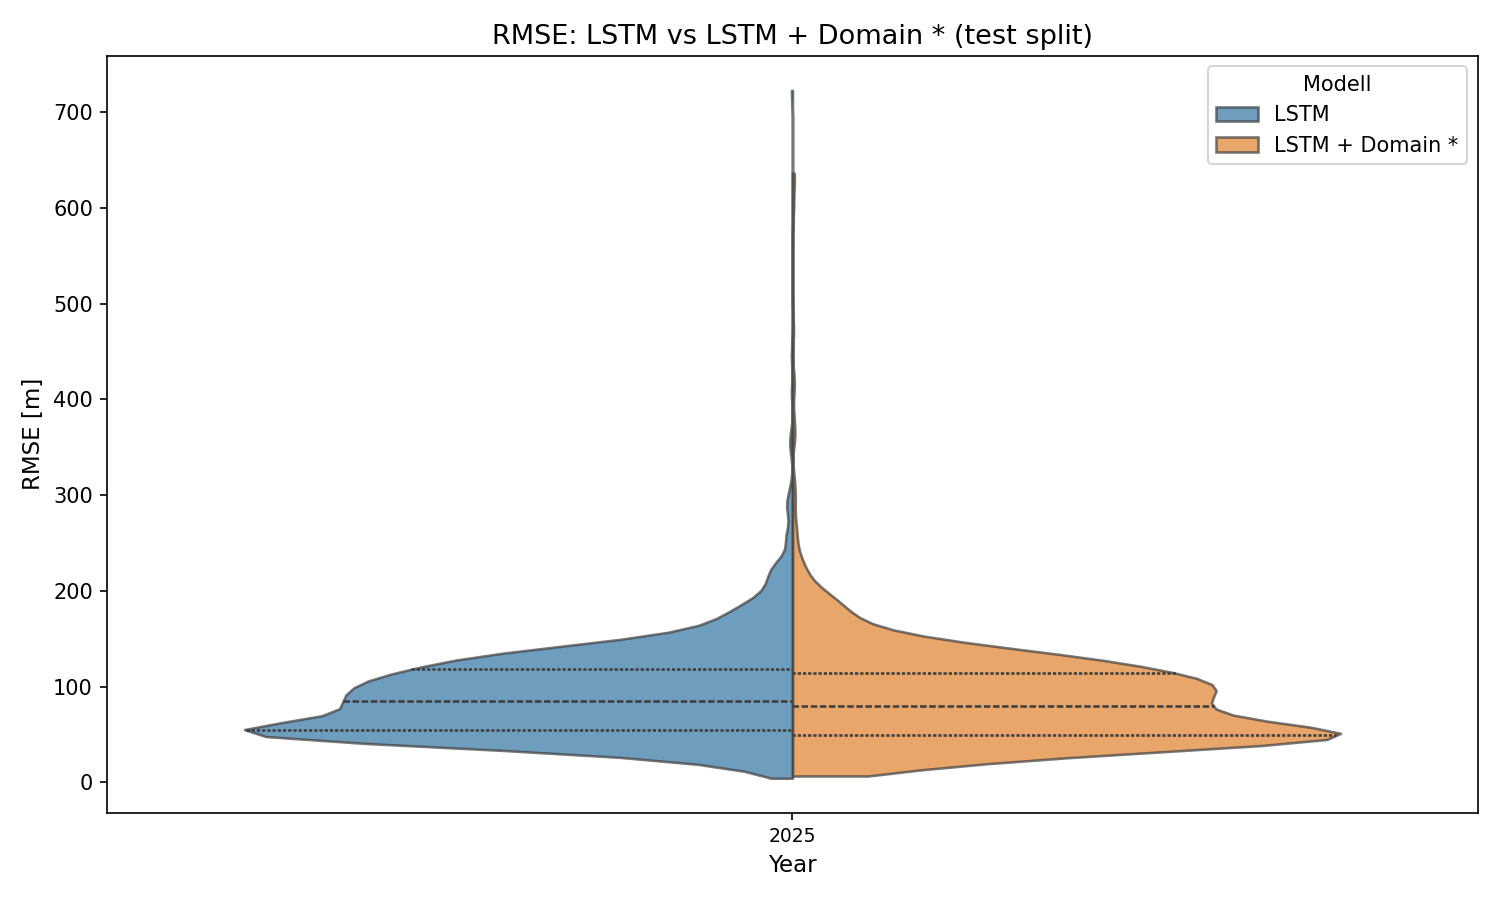
\includegraphics[width=0.6\linewidth]{figures/violindomaine.png}
    \caption[Exp. III RMSE Violin plot]{\ac{RMSE} violin plot comparing the standard \acf{LSTM} and the \ac{LSTM} + Domain* models on the full test set. \todo{replot with biiger captions once vera is online}}
    \label{fig:violindomaine}
\end{figure}

\begin{figure}
    \centering
    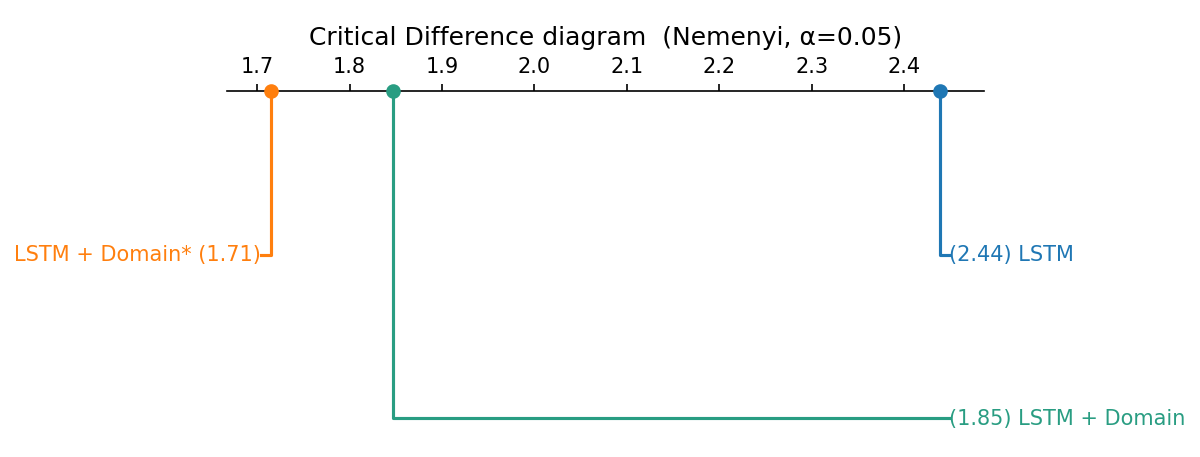
\includegraphics[width=0.6\linewidth]{figures/cd_diagram_lstm_comparison.png}
    \caption[Exp. III Friedman \& Nemenyi CD-Plot]{Critical Difference diagram comparing the \acf{LSTM} variants with and without Domain specific training. \ac{LSTM} + {OHE} refers to the \ac{LSTM} + Domain model. 
ac{LSTM} +{OHE}* refers to the \ac{LSTM} + Domain model that was run using the hyperparameters of the \ac{LSTM}
without any optimisation. }
    \label{fig:cd_exp3_real}
\end{figure}


\FloatBarrier

\subsection{Discussion}

Interestingly, the LSTM + Domain* model that reuses the hyperparameters of the baseline LSTM outperforms the LSTM + Domain model that was tuned in a separate Optuna study with statistical significance (Figure \ref{fig:cd_exp3}).
During the hyperparameter search for the standard LSTM + Domain model, the optimisation algorithm failed to find a better configuration than the initial 16 trials before early stopping terminated the study.
This indicates that the search likely stopped prematurely and that the domain-aware architecture could benefit from a more exhaustive tuning procedure.
Future work should revisit this experiment with increased patience or a larger hyperparameter optimisation budget to fully exploit the potential of the explicit domain encoding.

The consistent outperformance of the LSTM + Domain models against the standard \acp{LSTM} in Table \ref{tab:results_exp3} and Figure \ref{fig:violindomaine} indicates a clear and robust dominance of the domain-aware model over the baseline.
These results provide strong evidence that explicitly encoding domain information into the model architecture consistently improves trajectory prediction performance in all considered domains.
The domain-aware model has a lower median error and lower first and third quartiles, indicating consistently better typical performance. The interquartile ranges of both models are comparable, but the baseline \ac{LSTM} shows more extreme outliers. This suggests that the embeddings help in avoiding occasional large errors. Eliminating these outliers is exactly the primary objective when deploying trajectory forecasting models in safety-critical environments.
While the best-case \acs{RMSE} of the baseline is slightly lower in this particular run, this effect was not consistent across the additional ten training runs and does not affect the overall dominance of the domain-aware model. 

It should be highlighted that this experiment used a relatively naive domain encoding strategy across only a small number of distinct classes. Even more substantial performance improvements can be expected in future work by exploring more sophisticated encoding techniques or incorporating a broader variety of waterway environments. % conclusion?

%2nd versionW, still before feedback
%!TEX root=../main.tex
\chapter{Results and Discussion}%keine interpretation
\acresetall %reset abbrevations
\label{chap:results}


In this chapter, we present the findings from the experimental evaluation, and address the core research questions systematically.
The overall goal of these experiments was to provide a fair comparison of deep learning models, kinematic models, and stochastic filters, as well as to investigate the impact of incorporating geographic domain information into model training and architecture.
To evaluate the three research questions outlined in Section \ref{sec:rqand}, we conducted a total of three experiments: a baseline comparison of all motion models on the full dataset (Exp I), an assessment of the effect of domain-specific training on predictive performance (Exp II), and an ablation study of explicit domain encoding for LSTMs (Exp III).
The remainder of this chapter is structured around the  questions, for each of which we present the quantitative results first, along with the answers to our research questions. A more detailed discussion of the results follows.

The preprocessed dataset is provided at Hugging Face\footnote{\url{https://huggingface.co/datasets/kawihss/ais-inland-vessel-trajectories}}. 
The dataset can be regenerated with the pipeline provided at RWTH GitLab\footnote{\url{https://git-ce.rwth-aachen.de/g-nav-mob-irt/projects/galileonautic2plus/multi-object-tracking/motion-models/-/tree/handedIn}} or the public GitHub mirror\footnote{\url{https://github.com/kawihss/Data-based-vessel-motion-modelling-Thesis/tree/handedIn}}. 
The repository also provides the code to train and optimise all models. For details on the pipeline, refer to the readme files and Appendix~\ref{chap:appendixcodebase} for a general overview of the codebase architecture.

%\section[Exp. \Romannum{1}: Motion Model Comparison]{Exp. \Romannum{1}: Baseline Comparison of Motion Models} 

 
\textbf{RQ 1:} \textit{Given a preprocessed dataset and a systematic hyperparameter optimisation procedure, how do deep learning models, both task-specific and pretrained, kinematic baselines, and stochastic filters compare in short-term trajectory prediction of inland vessels?}

We set up Exp. \Romannum{1} to answer this question and to serve as an overall baseline comparison across all evaluated motion models and model families on the full dataset. 

\paragraph{Results.}
The optimised hyperparameter configurations for all evaluated models are listed in Table~\ref{tab:hpo_results_exp0}, and the corresponding test set error metrics are detailed in Table~\ref{tab:results_exp0}.
Specifically, the standard \ac{LSTM} achieves an \ac{ADE} of $54.78$\,m and a \acf{RMSE} of $111.36$\,m, reducing the error of the \ac{CV} baseline (\ac{ADE} $78.39$\,m, \ac{RMSE} $155.73$\,m) by $30.1\%$ and $28.5\%$, respectively.
To assess the overall statistical significance of these results, we conducted a Friedman test combined with Nemenyi post-hoc comparison.
The significant differences are illustrated as a \ac{CD} diagram in Figure~\ref{fig:cd_test}. 
The diagram reveals a clear ranking structure: the two LSTM-based models occupy the top positions, with average ranks of 1.5 and 2 respectively, followed by the \ac{EKF} (4.7) and Chronos-2 (5.4), while the remaining models form a middle group with mostly non-significant pairwise differences (6.4 -- 7).
The CTRV-based models rank last (8.1).



\begin{table}[t]
%\centering
\noindent
\caption[Exp. I Optimised Hyperparameter Configurations]{Optimised hyperparameter (HP) configurations for all models. Discussed parameters are shaded.}
\label{tab:hpo_results_exp0}
\begin{minipage}[t]{0.49\textwidth}
\centering
\begin{tabular}{llr}
\toprule
\textbf{Model} & \textbf{HP} & \textbf{Value} \\
\midrule
CV             & \cellcolor{blue!15}$n_\text{vel}$  & \cellcolor{blue!15}1 \\
CTRV           & $n_\text{vel}$                     & 2 \\
CTRV Arc       & $n_\text{vel}$                     & 3 \\
Hybrid         & $n_\text{vel}^\text{CV}$            & 1 \\
               & $n_\text{vel}^\text{CTRV}$          & 2 \\
               & $n_\text{rot}$                      & 1 \\
               & \cellcolor{blue!15}$\tau_\text{rot}$& \cellcolor{blue!15}29.28°/min \\
\midrule
KF (CV)        & \cellcolor{cyan!15}$q_\text{pos}$  & \cellcolor{cyan!15}$1.578{\times}10^{-3}$ \\
               & $q_\text{vel}$                     & $5.932$ \\
               & \cellcolor{cyan!15}$r_\text{pos}$  & \cellcolor{cyan!15}$1.077{\times}10^{-2}$ \\
               & $p_{0,\text{pos}}$                 & $7.737{\times}10^{-2}$ \\
               & $p_{0,\text{vel}}$                 & $1.190{\times}10^{-1}$ \\
\midrule
EKF (CTRV)     & \cellcolor{green!15}$q_\text{pos}$ & \cellcolor{green!15}$15.957$ \\
               & $q_\text{vel}$                     & $4.290{\times}10^{-2}$ \\
               & \cellcolor{green!15}$q_\text{rot}$ & \cellcolor{green!15}$1.002{\times}10^{-7}$ \\
               & $r_\text{pos}$                     & $1.792{\times}10^{-2}$ \\
               & $p_{0,\text{pos}}$                 & $4.046{\times}10^{-1}$ \\
               & $p_{0,\text{vel}}$                 & $1.845{\times}10^{-3}$ \\
               & $p_{0,\text{rot}}$                 & $2.076{\times}10^{-6}$ \\
               & $n_\text{ctx}$                     & 2 \\
\bottomrule
\end{tabular}
\end{minipage}
%\hfill
\begin{minipage}[t]{0.40\textwidth}
\centering
\begin{tabular}{llr}
\toprule
\textbf{Model} & \textbf{HP} & \textbf{Value} \\
\midrule
Chronos-2      & \multicolumn{2}{l}{\textit{no HPO}} \\
TiRex          & context length          & 1 \\
\midrule
LSTM           & hidden size             & 256 \\
               & num.\ layers            & 2 \\
               & dropout                 & 0.290 \\
               & learning rate           & $5.530{\times}10^{-4}$ \\
               & batch size              & 128 \\
               & \cellcolor{orange!15}feature set & \cellcolor{orange!15}no rot \\
\midrule
LSTM+Domain    & hidden size             & 256 \\
               & num.\ layers            & 2 \\
               & dropout                 & 0.300 \\
               & learning rate           & $4.000{\times}10^{-4}$ \\
               & batch size              & 256 \\
               & feature set             & all \\
\bottomrule
\end{tabular}
\end{minipage}
\end{table}


\begin{table}[t]
\centering
\caption[Exp. I Test Set Error Metrics] {Test set error metrics for all models}%Discussed metrics shaded in.}
\label{tab:results_exp0}
\begin{tabular}{lrrr}
\toprule
\textbf{Model} & \textbf{ADE} & \textbf{FDE} & \textbf{RMSE} \\
\midrule
CV                  & 78.39 & 175.82 & 155.73 \\
CTRV                & 82.92 & 195.18 & 164.51 \\
CTRV Arc            & 85.21 & 196.78 & 168.29 \\
Hybrid CV/CTRV      & 78.49 & 176.45 & 155.49 \\
\midrule
KF (CV)             & 78.39 & 175.82 & 155.73 \\
EKF (CTRV)          & 78.94 & 174.88 & 151.50 \\
\midrule
Chronos-2           & 80.25 & 179.80 & 152.86 \\
TiRex               & 78.37 & 175.82 & 155.71 \\
\midrule
LSTM                & 54.78 & 121.18 & 111.36 \\
LSTM + Domain       & 53.80 & 119.02 & 109.95 \\
\bottomrule
\end{tabular}
\end{table}

\begin{figure}[h]
    \centering
    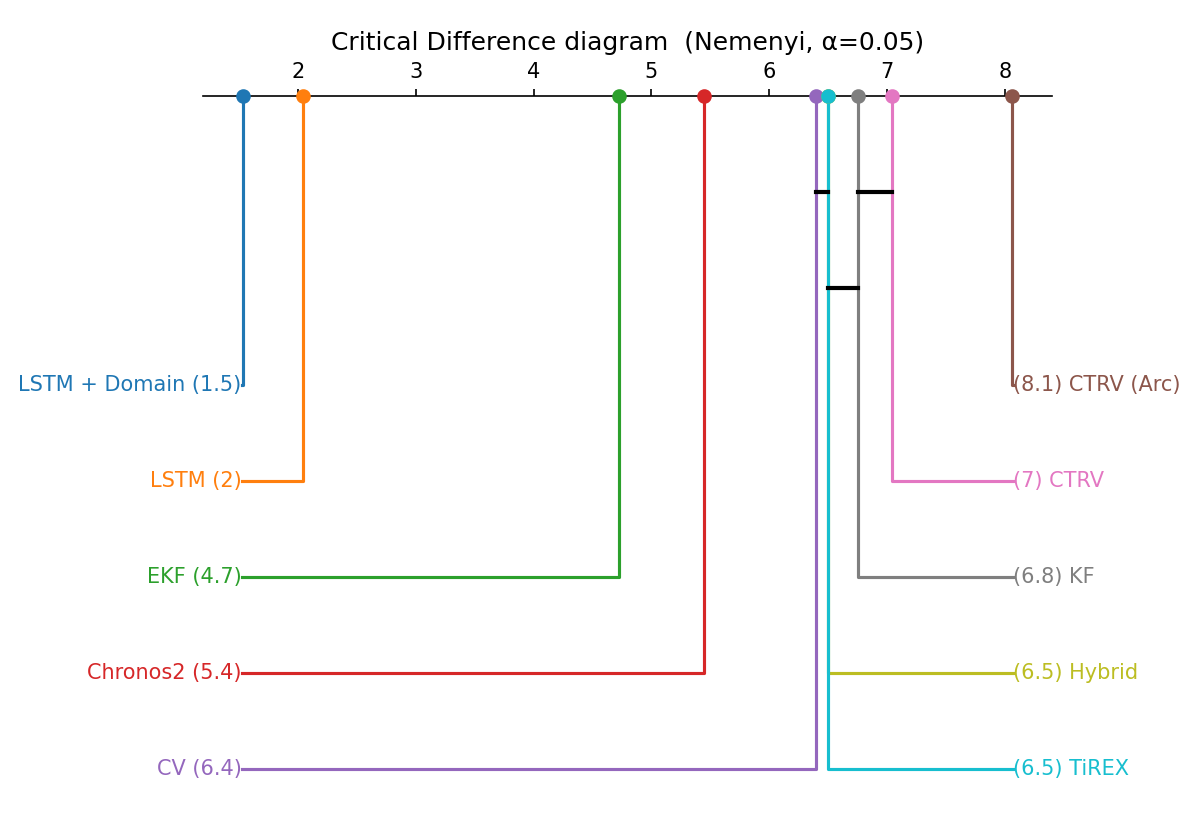
\includegraphics[width=0.7\linewidth]{figures/cd_diagram.png}
    \caption[Exp. I Friedman \& Nemenyi CD-Plot]{ \acf{CD} diagram based on the Friedman test and Nemenyi post-hoc comparison. Models connected by a horizontal bar are not significantly different at \( \alpha = 0.05\). The shown numbers are the mean rank per model in the evaluation, 1 being the best possible result.}
    \label{fig:cd_test}
\end{figure}

Figure~\ref{fig:adepredhorizon} depicts the development of the \ac{ADE} for all models over the prediction horizon. While the error for the \ac{CV} model grows approximately linearly, the errors for CTRV and CTRV Arc diverge heavily at longer horizons. The \ac{LSTM}-based models maintain the lowest \ac{ADE} across all ten prediction steps. The ranking order of all models stays consistent over the full horizon.

\begin{figure}[h]
    \centering
    \begin{tikzpicture}
    \begin{axis}[
        width=0.78\linewidth,
        height=6cm,
        xlabel={Prediction Step},
        ylabel={ADE (m)},
        xmin=1, xmax=10,
        xtick={1,2,...,10},
        ymin=0,
        grid=major,
        grid style={dashed, gray!30},
        legend style={
            at={(0.5,-0.28)},
            anchor=north,
            legend columns=4,
            font=\small
        },
        mark size=1.5pt,
        cycle list name=color list,
    ]
    
    \addplot coordinates {
        (1,7.861)(2,16.747)(3,28.983)(4,43.096)(5,60.103)
        (6,78.936)(7,100.214)(8,123.386)(9,148.728)(10,175.824)
    }; \addlegendentry{CV}
    
    \addplot coordinates {
        (1,8.353)(2,16.865)(3,28.177)(4,42.303)(5,59.811)
        (6,80.468)(7,104.477)(8,131.658)(9,161.924)(10,195.180)
    }; \addlegendentry{CTRV}
    
    \addplot coordinates {
        (1,8.976)(2,18.242)(3,30.422)(4,45.051)(5,62.918)
        (6,83.636)(7,107.548)(8,134.347)(9,164.148)(10,196.783)
    }; \addlegendentry{CTRV Arc}
    
    \addplot coordinates {
        (1,8.054)(2,16.930)(3,29.044)(4,43.019)(5,59.942)
        (6,78.772)(7,100.143)(8,123.486)(9,149.066)(10,176.446)
    }; \addlegendentry{Hybrid CV/CTRV}
    
    \addplot coordinates {
        (1,7.861)(2,16.747)(3,28.983)(4,43.096)(5,60.103)
        (6,78.936)(7,100.216)(8,123.386)(9,148.726)(10,175.824)
    }; \addlegendentry{KF (CV)}
    
    \addplot coordinates {
        (1,8.364)(2,17.853)(3,30.191)(4,44.472)(5,61.235)
        (6,79.889)(7,100.747)(8,123.511)(9,148.295)(10,174.882)
    }; \addlegendentry{EKF (CTRV)}
    
    \addplot coordinates {
        (1,8.020)(2,17.405)(3,29.932)(4,44.419)(5,61.698)
        (6,80.865)(7,102.417)(8,126.026)(9,151.936)(10,179.800)
    }; \addlegendentry{Chronos-2}
    
    \addplot coordinates {
        (1,7.860)(2,16.743)(3,28.975)(4,43.083)(5,60.084)
        (6,78.911)(7,100.189)(8,123.362)(9,148.711)(10,175.820)
    }; \addlegendentry{TiRex}
    
    \addplot coordinates {
        (1,5.769)(2,12.005)(3,20.515)(4,30.700)(5,42.527)
        (6,55.682)(7,70.279)(8,86.083)(9,103.057)(10,121.181)
    }; \addlegendentry{LSTM}

    \addplot coordinates {
        (1,5.686)(2,11.776)(3,20.143)(4,30.110)(5,41.737)
        (6,54.729)(7,69.035)(8,84.572)(9,101.244)(10,119.017)
    }; \addlegendentry{LSTM + Domain}
    
    \end{axis}
    \end{tikzpicture}
    %\caption{ADE per prediction step averaged across all tracks 
    \caption[Exp. I ADE over Time]{Progression of \acf{ADE} over time, showing the divergence of error across all ten prediction steps. The plot demonstrates that \acf{LSTM}-based architectures achieve the lowest errors, while kinematic models exhibit higher trajectory divergence, particularly as the prediction horizon increases.}
    \label{fig:adepredhorizon}
\end{figure} 

Regarding the foundation models, Table~\ref{tab:results_exp0_foundation_prob} shows the probabilistic calibration metrics.
TiRex produces extremely narrow prediction intervals (Mean Interval Width of 6.41) and achieves a coverage of only 0.059. In contrast, Chronos-2 produces wider intervals (Mean Interval Width of 145.37) but achieves a near-ideal coverage of 0.769. %\me{move calibration to discussion?}
Figure~\ref{fig:violince} visualises the error distribution shapes as violin plots, showing that TiRex and the \ac{CV} model share nearly identical error distributions, while the \ac{LSTM} distribution is distinctly shifted toward lower errors.

Furthermore, an evaluation of the error distributions for the kinematic baselines (\ac{CV} and \ac{CTRV}) reveals a stark deviation from a normal distribution, with coefficients of determination ($R^2$) ranging from 0.6138 to 0.6428.

\begin{table}[t]
\centering
\caption{Exp. I Probabilistic metrics for foundation models}
\label{tab:results_exp0_foundation_prob}
\begin{tabular}{lrrr}
\toprule
\textbf{Model} & \textbf{MIW} & \textbf{Coverage} & \textbf{Winkler80} \\
\midrule
Chronos-2 (zero-shot) & 145.37 & 0.769 & 114.65 \\
TiRex                 &   6.41 & 0.059 & 112.20 \\
\bottomrule
\end{tabular}
\end{table}

\begin{figure}[h]
    \centering
    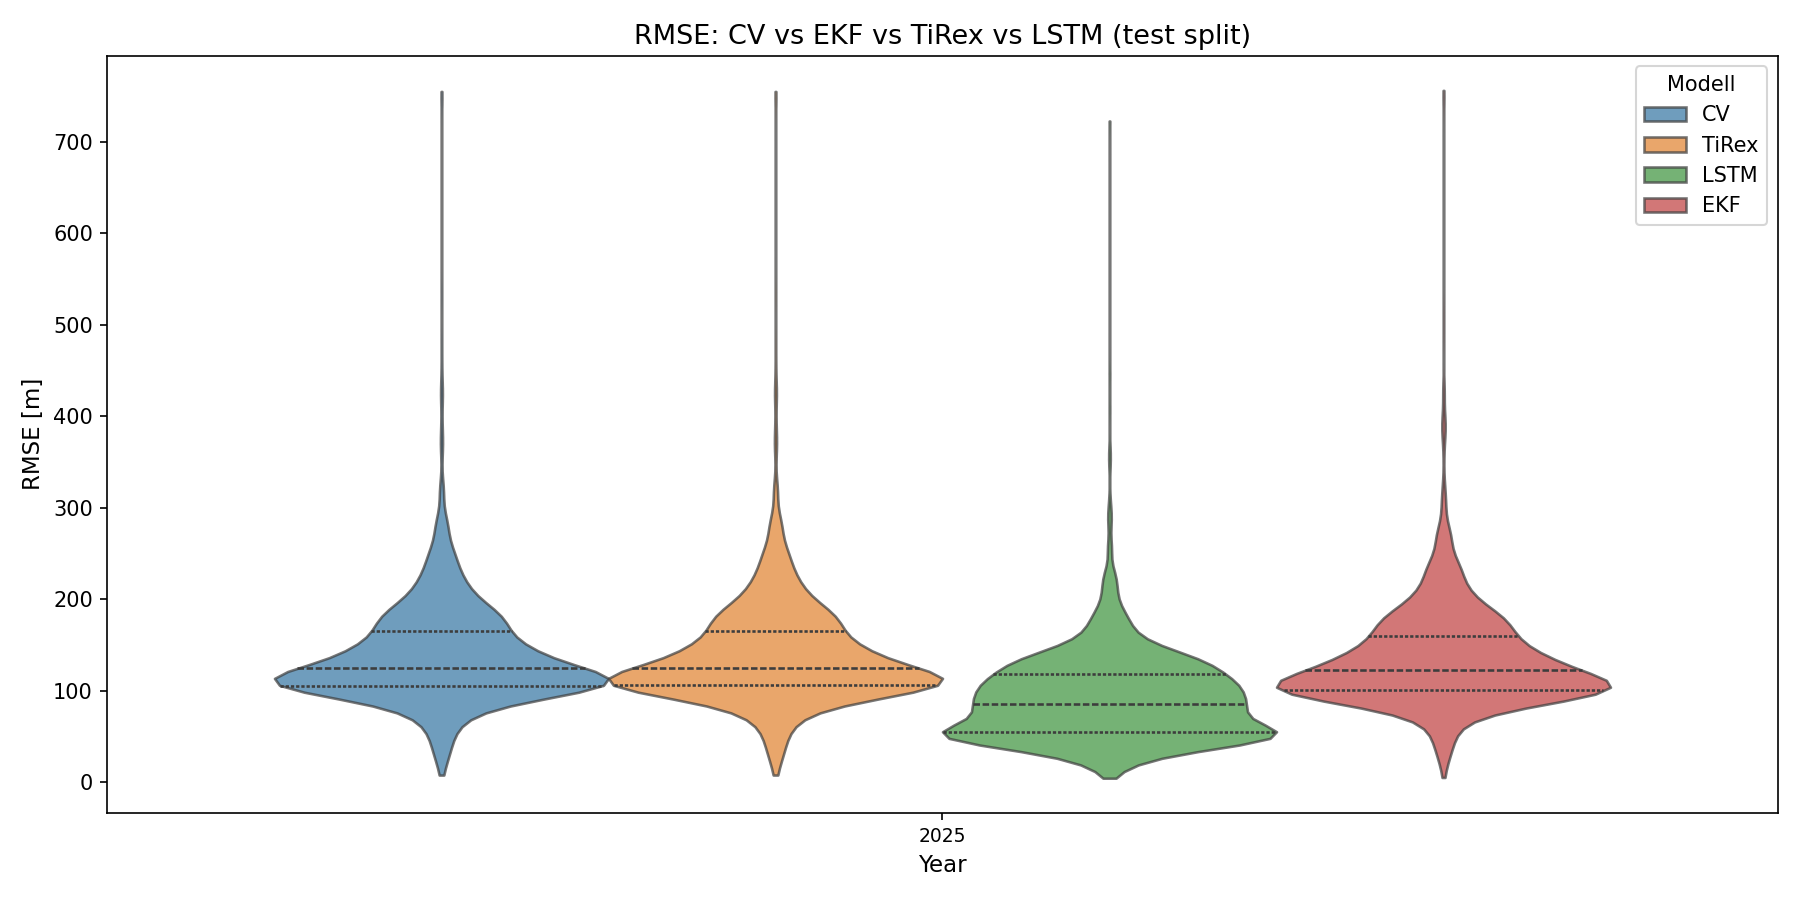
\includegraphics[width=0.98\linewidth]{test_violin_cv_ekf_tirex_lstm_per_year.png}
    %\caption{Violin Plots for CV, EKF, TiRex and LSTM}
    \caption[Exp. I RMSE Violin Plots]{Violin plots visualising the distribution of \acf{RMSE} for the \acf{CV}, \acf{EKF}, TiRex, and \acf{LSTM} models on the test set. The \ac{LSTM} model demonstrates a distinct shift toward lower error values compared to the other models, whereas the \acf{CV} and TiRex models exhibit nearly identical error distributions.}
    \label{fig:violince}
\end{figure}

Finally, the hyperparameter optimisation process for the \ac{LSTM} is visualised in % Figure ~\ref{fig:succhalfing} and
Figure~\ref{fig:paralelcord}. 
% Figure~\ref{fig:succhalfing} illustrates a successive halving run, demonstrating how underperforming configurations were pruned early.
%Figure~\ref{fig:paralelcord} 
It presents a parallel coordinate plot of the parameter search with a clear band around the optimal configuration. The plot indicates that the optimisation selected a feature set that explicitly excluded the \ac{ROT}.
Furthermore, Figure~\ref{fig:monthlytrends-all} plots the average \ac{RMSE} per month over the full dataset, with consistent performance trends across all models.

%\begin{figure}[h]
%    \centering
%    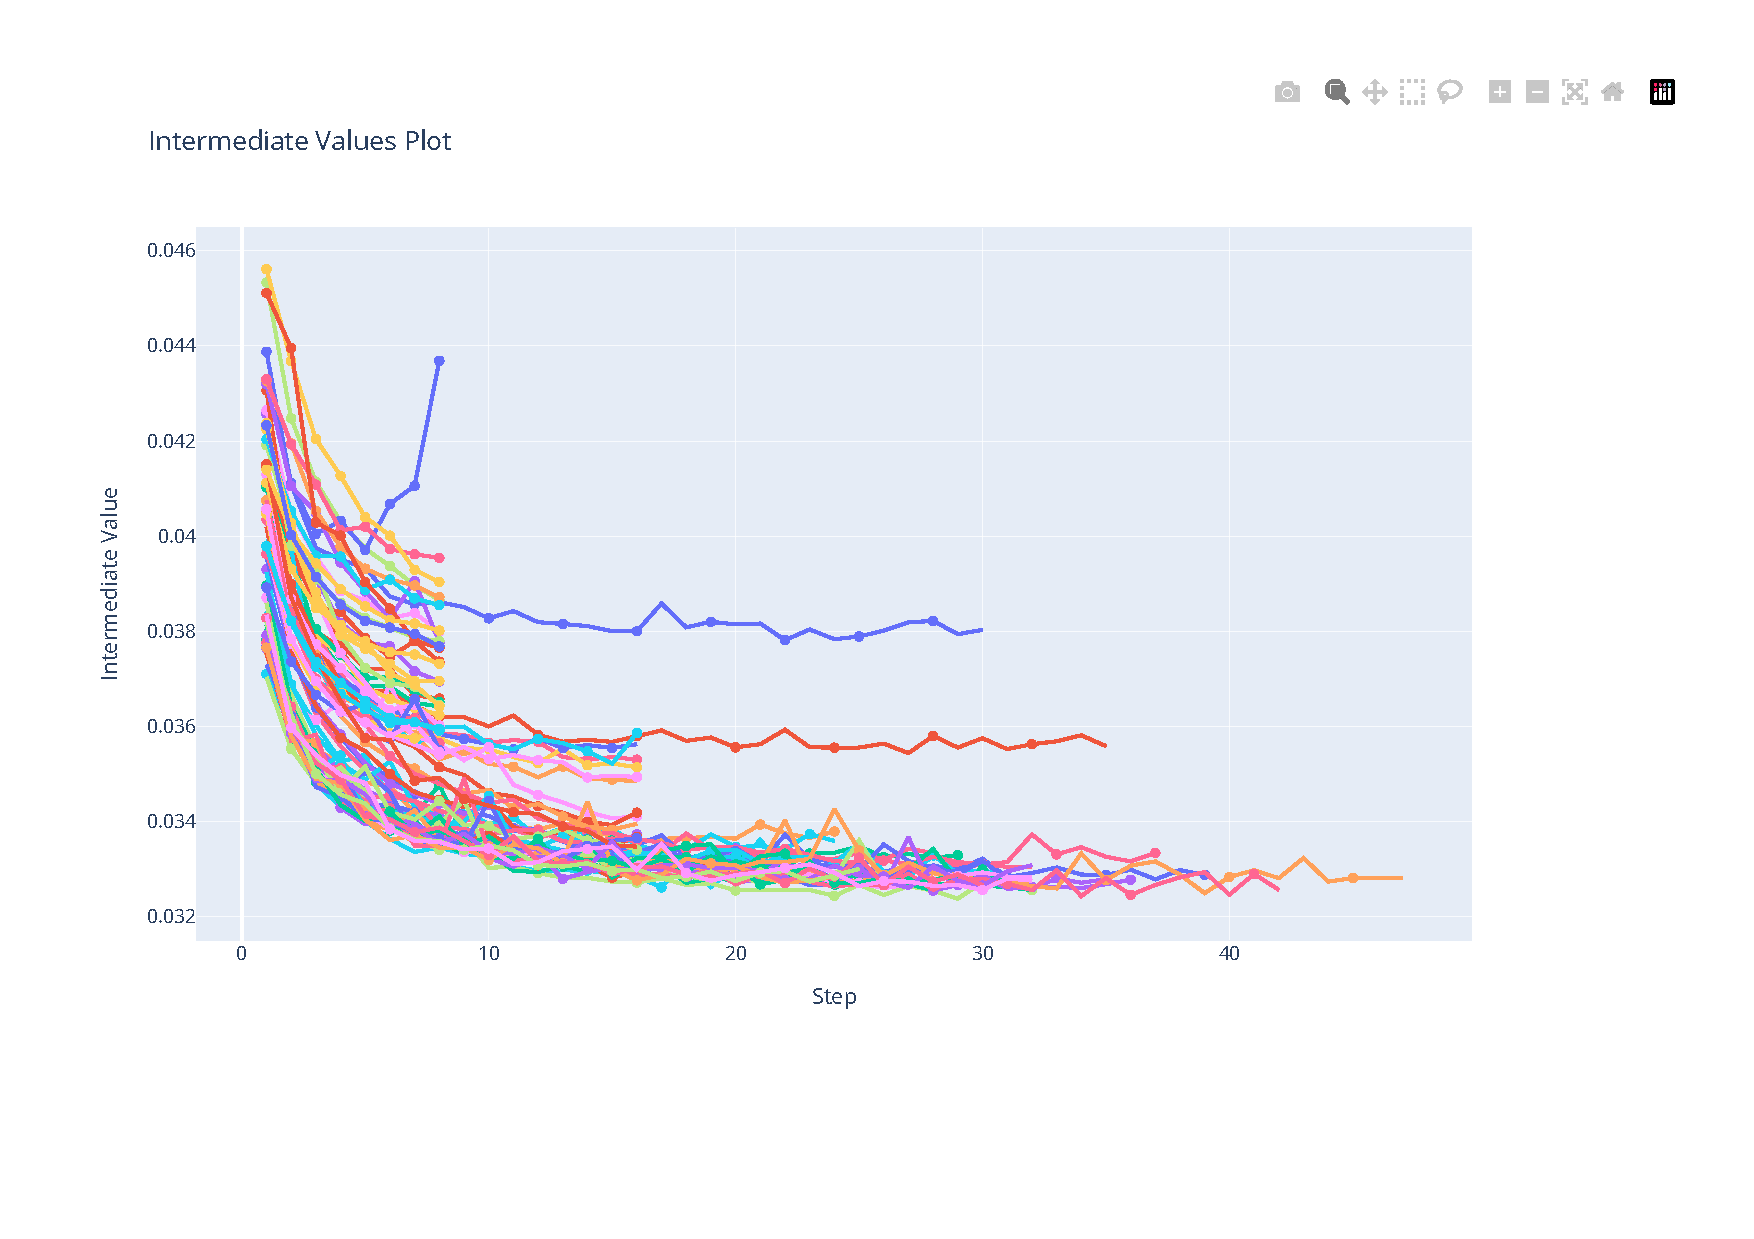
\includegraphics[width=0.9\linewidth,trim=1cm 3.5cm 5.5cm 3.5cm,clip]{figures/minimal_lstm_intermediate_values.html.pdf}
%    \caption[Exp. I LSTM Intermediate Value plot]{Intermediate Value plot of \acf{LSTM} \acf{HPO} in Optuna with early stopping enabled. Successive Halving was applied to all trials, except the initial 16. \me{should this be moved into methods, appendix? removed? it is not discussed in detail} \todo{remove all result references to this}}
%    \label{fig:succhalfing}
%\end{figure}

\begin{figure}[h]
    \centering
    %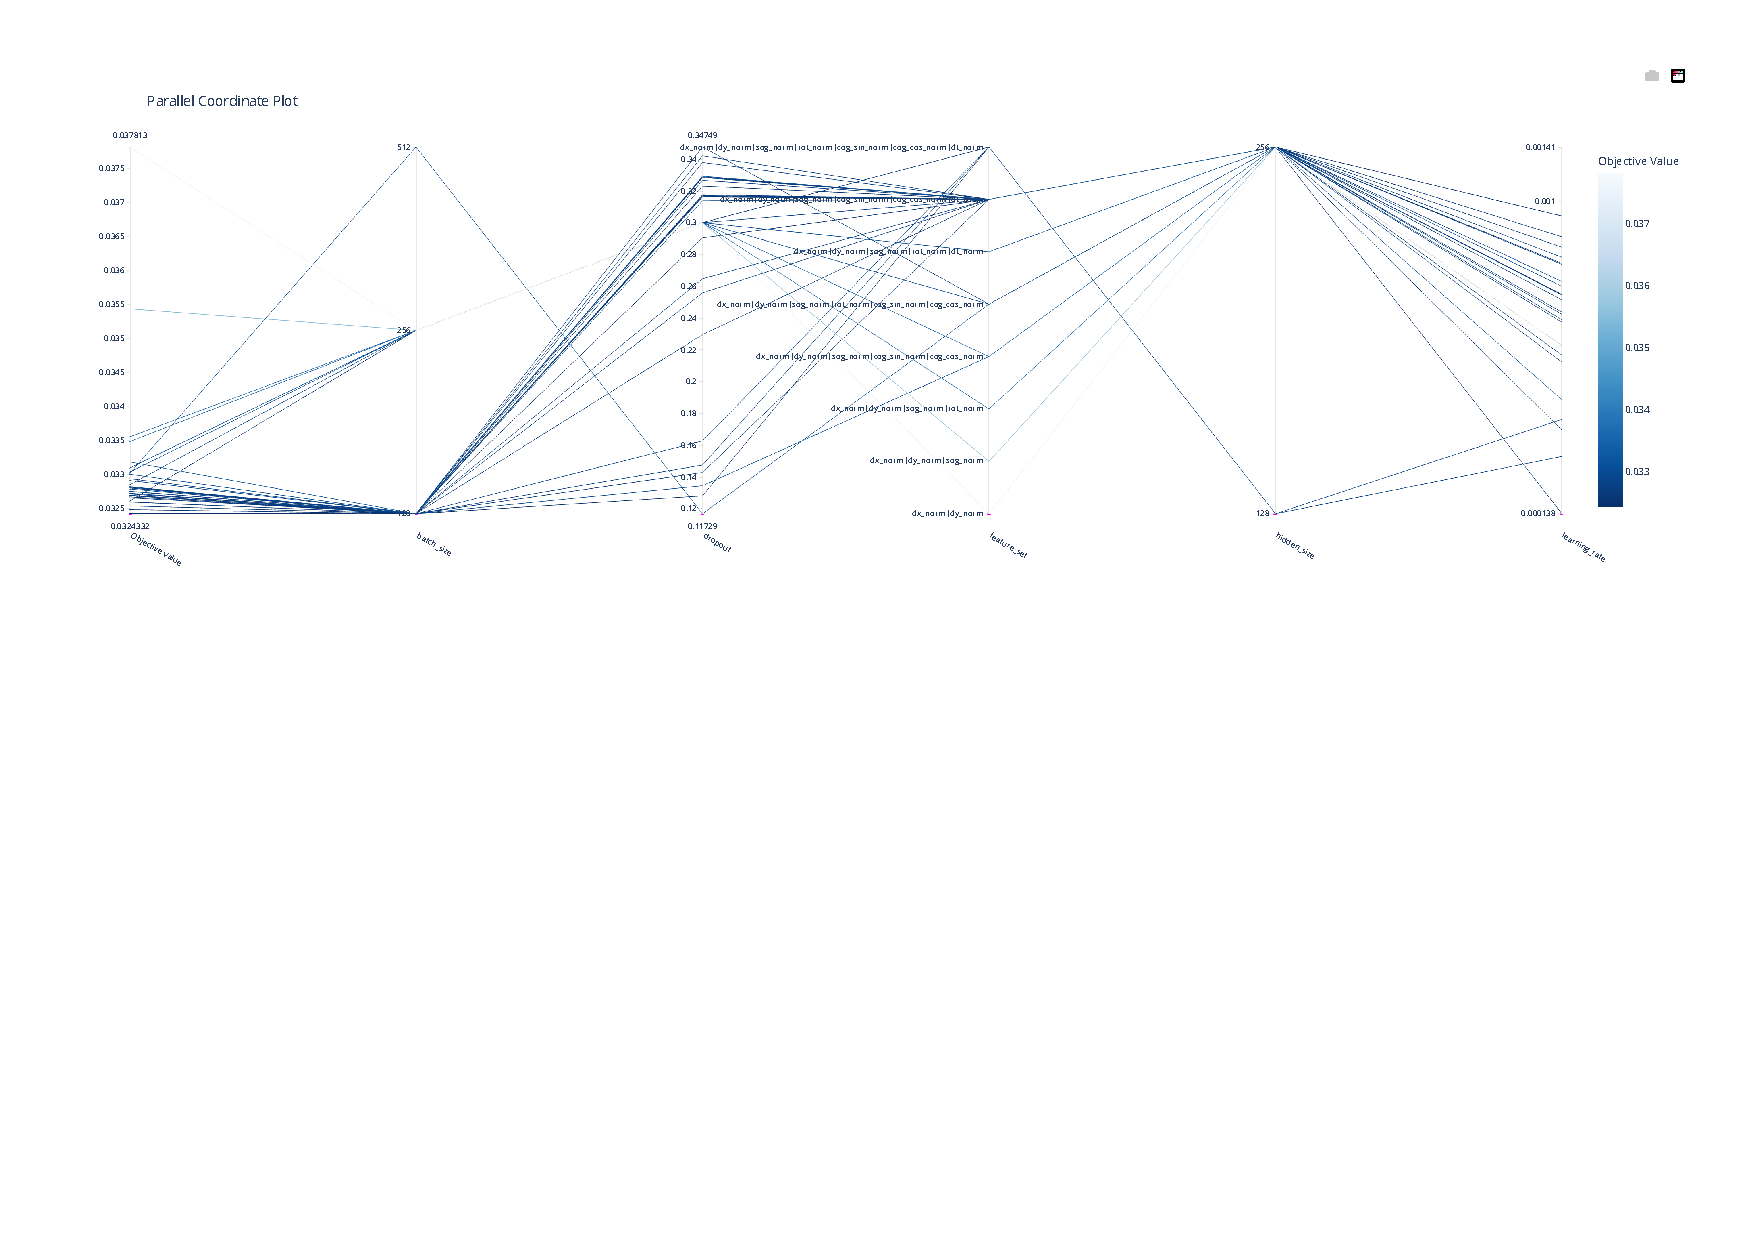
\includegraphics[width=1\linewidth,trim=1cm 10.5cm 1cm 1.5cm,clip]{figures/minimal_lstm_parallel_coordinate.html.pdf}
    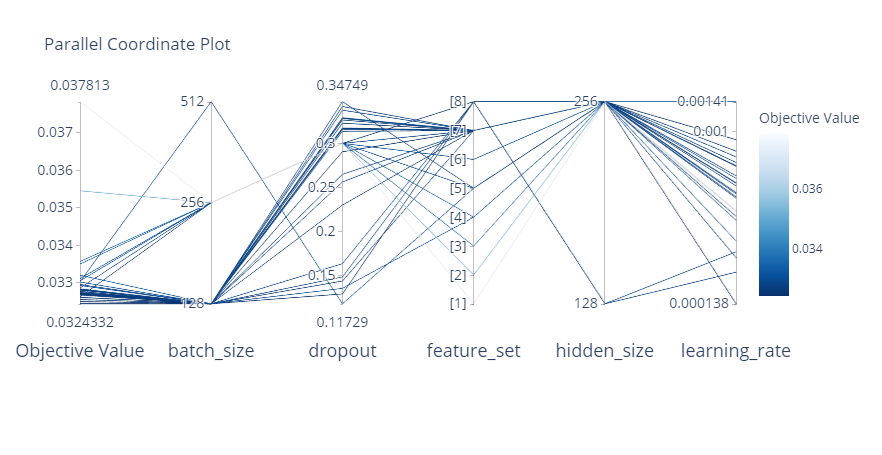
\includegraphics[width=1\linewidth, trim=0cm 3.1cm 0cm 2cm,clip]{figures/paralelcoord_zoomed.png}
    %\caption[Exp. I LSTM Parallel Coordinate Plot]{Parallel Coordinate Plot of \acf{LSTM} Hyperparameter selection, showing a clear band around the selected hyperparameter configuration. \todo{add 1, 2, 3...}}
    \caption[Exp. I LSTM Parallel Coordinate Plot]{Parallel Coordinate Plot of \acf{LSTM} Hyperparameter selection, showing a clear band around the selected hyperparameter configuration. Feature set mappings: [1] dx\_norm, dy\_norm; [2] dx\_norm, dy\_norm, sog\_norm; [3] dx\_norm, dy\_norm, sog\_norm, rot\_norm; [4] dx\_norm, dy\_norm, sog\_norm, cog\_sin\_norm, cog\_cos\_norm; [5] dx\_norm, dy\_norm, sog\_norm, rot\_norm, cog\_sin\_norm, cog\_cos\_norm; [6] dx\_norm, dy\_norm, sog\_norm, rot\_norm, dt\_norm; [7] dx\_norm, dy\_norm, sog\_norm, cog\_sin\_norm, cog\_cos\_norm, dt\_norm; [8] dx\_norm, dy\_norm, sog\_norm, rot\_norm, cog\_sin\_norm, cog\_cos\_norm, dt\_norm.} \me{new version with increased font sizes and feature sets not witten explcicitly because of overlap. now the caption is very long though, any ideas?}
    \label{fig:paralelcord}
\end{figure}


\begin{figure}[h]
    \centering
    \begin{tikzpicture}
    \begin{axis}[
        name=main,
        width=0.85\linewidth,
        height=8cm, 
        xlabel={Month},
        ylabel={RMSE (m)},
        ymin=75, ymax=175, 
        xmin=0.5, xmax=12.5,
        xtick={1,2,...,12},
        xticklabels={Jan,Feb,Mar,Apr,May,Jun,Jul,Aug,Sep,Oct,Nov,Dec},
        xticklabel style={rotate=45, anchor=east, font=\small},
        grid=major,
        grid style={dashed, gray!30},
        legend style={
            at={(0.5,-0.22)},
            %at={(0.5, 1.1)},
            anchor=north,
            legend columns=4,
            font=\small
        },
        mark size=1.5pt,
        cycle list name=color list,
        axis y line*=left,
        axis x line*=bottom,
    ]
    
    \addplot coordinates {
        (1,150.68)(2,146.54)(3,145.76)(4,148.09)(5,134.58)
        (6,130.30)(7,127.56)(8,133.85)(9,133.55)(10,143.01)
        (11,134.22)(12,134.11)
    }; \addlegendentry{CV}
    
    \addplot coordinates {
        (1,154.44)(2,150.62)(3,151.49)(4,153.95)(5,138.43)
        (6,135.97)(7,133.14)(8,138.42)(9,137.73)(10,149.36)
        (11,139.39)(12,136.40)
    }; \addlegendentry{CTRV}
    
    \addplot coordinates {
        (1,160.16)(2,155.51)(3,156.69)(4,159.50)(5,142.50)
        (6,139.55)(7,136.44)(8,142.23)(9,142.46)(10,153.20)
        (11,143.27)(12,141.02)
    }; \addlegendentry{CTRV Arc}
    
    \addplot coordinates {
        (1,151.39)(2,147.01)(3,146.20)(4,147.73)(5,134.67)
        (6,131.39)(7,127.38)(8,134.15)(9,134.07)(10,143.37)
        (11,133.93)(12,133.65)
    }; \addlegendentry{Hybrid CV/CTRV}
    
    \addplot coordinates {
        (1,150.68)(2,146.54)(3,145.76)(4,148.09)(5,134.58)
        (6,130.30)(7,127.56)(8,133.85)(9,133.55)(10,143.01)
        (11,134.22)(12,134.11)
    }; \addlegendentry{KF (CV)}
    
    \addplot coordinates {
        (1,146.42)(2,142.48)(3,141.74)(4,144.76)(5,130.69)
        (6,126.45)(7,124.73)(8,130.01)(9,130.24)(10,139.55)
        (11,130.87)(12,130.29)
    }; \addlegendentry{EKF (CTRV)}
    
    \addplot coordinates {
        (1,146.06)(2,143.09)(3,141.57)(4,143.28)(5,130.72)
        (6,124.68)(7,126.37)(8,129.56)(9,132.99)(10,140.82)
        (11,131.24)(12,130.51)
    }; \addlegendentry{Chronos-2}
    
    \addplot coordinates {
        (1,150.65)(2,146.52)(3,145.73)(4,148.08)(5,134.58)
        (6,130.29)(7,127.55)(8,133.85)(9,133.54)(10,143.00)
        (11,134.21)(12,134.09)
    }; \addlegendentry{TiRex}
    
    \addplot coordinates {
        (1,98.00)(2,93.24)(3,96.86)(4,93.53)(5,90.71)
        (6,83.01)(7,87.67)(8,89.58)(9,90.85)(10,97.84)
        (11,87.86)(12,90.82)
    }; \addlegendentry{LSTM}

    \addplot coordinates {
        (1,90.84)(2,86.57)(3,93.25)(4,91.92)(5,85.43)
        (6,79.95)(7,83.18)(8,85.01)(9,86.97)(10,92.49)
        (11,83.83)(12,86.24)
    }; \addlegendentry{LSTM + Domain}
    
    \end{axis}
    
    \begin{axis}[
        width=0.85\linewidth,
        height=8cm,
        ymin=0, ymax=160000,
        xmin=0.5, xmax=12.5,
        xtick=\empty,
        ylabel={$n_\text{samples}$},
        ylabel style={at={(1.08,0.5)}, color=violet},
        ytick={0,40000,80000,120000},
        yticklabels={0,40k,80k,120k},
        yticklabel style={font=\small, color=violet},
        ytick style={color=cyan},
        axis y line*=right,
        axis x line=none,
        bar width=0.55,
    ]
    
    \addplot[ybar, fill=violet, draw=none, fill opacity=0.25] coordinates {
        (1,73177)(2,61903)(3,75120)(4,71784)(5,83023)
        (6,82636)(7,93205)(8,106326)(9,86547)(10,71582)
        (11,64072)(12,53443)
    };
    
    \end{axis}
    \end{tikzpicture}
    %\caption{RMSE per month with track count shown as violet bars\todo{from here on, expand figure and table captions}}
    \caption[Exp. I RMSE Monthly Trends]{Comparison of \acf{RMSE} by month, demonstrating consistent performance trends across all models. Violet bars indicate the monthly volume of samples}
    \label{fig:monthlytrends-all}
\end{figure}



%\section[Exp. \Romannum{2}: Domain-specific training]{Exp. \Romannum{2}: Effect of Domain-Specific Training on Predictive Performance}

%This experiment is designed to answer 
\FloatBarrier
\textbf{RQ 2}: \textit{Does domain-specific training improve short-term vessel trajectory prediction performance compared to mixed-domain training?}

We set up Exp. \Romannum{2} to evaluate the extent of these performance differences and how they are influenced by both the specific waterway domain and the underlying model complexity. %To that end, we set up Exp. \Romannum{2}.
\paragraph{Results.}

%performance between training modes
%The benefit of per-domain training increases with model complexity. %not purely descriptive
For the \ac{CV} model, no change in performance ($0.00$\,m difference) is observed between mixed and domain-specific training. Since the \ac{CV} search space consists of the single hyperparameter $n_\text{vel}$, and the optimiser converged to $n_\text{vel}=1$ in every domain as well as in the mixed setting, the resulting models are identical across all training regimes. The \ac{CTRV} variants exhibit deviations of up to $12.55$\,m in \ac{RMSE}. 
For the \ac{EKF} and \ac{LSTM}, however, substantial performance drops occur under mixed training, particularly in the channel and lock domains (Table \ref{tab:results_exp1_exp2_merged_deltas}, shaded in orange).
 Specifically, in the lock domain, the \ac{ADE} of the \ac{LSTM} degrades by $13.36$\,m and the \ac{RMSE} by $13.11$\,m when evaluated with the mixed training model.
This performance difference is not uniform across domains: in the harbour and river domains, only minor deviations are observed, generally remaining below a $5.6$\,m difference in \ac{RMSE}.
Finally, it can be observed that the harbour domain is the only environment where domain-specific training fails to produce a statistically significant improvement for the \ac{LSTM}. Further details about the statistical significance across domains can be found in Figure \ref{fig:cd-diagrams-a} in Appendix \ref{chap:appendixdataplots}.


%performance between domains
In Table~\ref{tab:results_exp1_exp2_merged_deltas}, the corresponding test set error metrics evaluated per domain are presented on the left, alongside the performance delta when evaluating the mixed training model on the right. Positive deltas indicate better performance for the models optimised on domain-specific data.
The lowest absolute errors are achieved in the channel domain; notably, the \ac{LSTM} attains an \ac{ADE} of $32.09$\,m and an \ac{RMSE} of $55.85$\,m (shaded in cyan).
Conversely, the highest errors are consistently produced in the harbour domain (e.g., an \ac{LSTM} \ac{ADE} of $61.07$\,m), making it comparatively difficult to predict.
When comparing model families, the largest relative improvements are observed in the lock and channel domains when moving from kinematic models to learned models. Changes in the harbour domain are inconsistent, with only minor improvements for the \ac{LSTM} and measurable degradation for the \ac{EKF} (a delta of $-1.47$\,m \ac{RMSE}).

%hyperparameters
In Table~\ref{tab:hpo_results_merged}, the optimised hyperparameter configurations for both mixed and domain-specific training setups are listed.
Notably, the optimised hyperparameters vary substantially across the domains.
This applies not only to the learned models but also to the Kalman filters. The optimised values for measurement noise, process noise, and initial covariance differ considerably. 
The measurement noise $r_\text{pos}$ covers nearly five orders of magnitude across models and domains, ranging from approximately $1.0\times10^{-2}$ to $7.3\times10^{2}$.
In particular, highly distinct parameter selections are yielded by the lock class for all models.
For example, very distinct hyperparameters can be observed for the \ac{LSTM} (such as a reduced hidden size of $64$ and an increased batch size of $512$). The \ac{EKF} applied to this domain is assigned a larger measurement noise $r_\text{pos}$ coupled with a very small process noise $q_\text{pos}$ (both shaded in green). 
Similarly, for TiRex and \ac{EKF}, a longer context length is selected specifically for the channel domain ($n_\text{ctx} = 9$ and $6$, respectively), while for kinematic baselines, the context length is reduced (shaded in cyan). %these are not discussed further, focus is on "yes there is a difference and it impacts performance" and not on "these are the differences and here is what it tells us about the data. in general, lots more can be discussed about specific parameters . eg how higher context windows act as a smoothness factor etc. but if we wanted to do that, we wouldnt have hpoed everything automatically
For the lock domain, in contrast, the \ac{EKF}'s context length is reduced to $n_\text{ctx}=1$. With only a single observation available before prediction begins, the filter has little opportunity to correct its $\omega_0=0$ initialisation if the vessel is already turning. Combined with the low process noise $q_\text{pos}$ and high measurement noise $r_\text{pos}$ discussed above, the filter is effectively optimised to trust its motion assumption over new measurements, which likely contributes to the disproportionately large performance gap between the \ac{EKF} and the \ac{LSTM} specifically in this domain.

\begin{comment}
\begin{table}[t]
\centering
\caption[Exp. II Optimised Hyperparameter Configurations]{Optimised hyperparameter configurations for per-domain training and mixed training. Discussed parameters are shaded in.}
\label{tab:hpo_results_merged}
\small
\setlength{\tabcolsep}{3pt}
\begin{tabular}{llrrrrr}
\toprule
\textbf{Model} & \textbf{Hyperparameter} & \textbf{Mixed} & \textbf{Harbour} & \textbf{River} & \textbf{Channel} & \textbf{Lock} \\
\midrule
CV             & $n_\text{vel}$        & 1      & 1     & 1     & 1     & 1     \\
CTRV           & $n_\text{vel}$        & 2      & 2     & 2     & \cellcolor{cyan!15}1     & 1     \\
CTRV Arc       & $n_\text{vel}$        & 3      & 3     & 3     & \cellcolor{cyan!15}2     & 1     \\
Hybrid CV/CTRV & $n_\text{vel}$ (CV)   & 1      & 1     & 1     & 1     & 1     \\
               & $n_\text{vel}$ (CTRV) & 2      & 2     & 2     & \cellcolor{cyan!15}1     & \cellcolor{orange!15}9     \\
               & $n_\text{rot}$        & 1      & 1     & 1     & 1     & \cellcolor{orange!15}9     \\
               & $\tau_\text{rot}$     & 29.28  & 29.28 & 29.28 & 1.00  & \cellcolor{orange!15}72.76 \\
\midrule
KF (CV)        & $q_\text{pos}$        & $1.578 \times 10^{-3}$ & $1.578 \times 10^{-3}$ & $2.434 \times 10^{-3}$ & $2.483 \times 10^{-3}$ & $1.578 \times 10^{-3}$ \\
               & $q_\text{vel}$        & $5.932$                & $5.932$                & $5.115$                & $9.930$                & $5.932$                \\
               & $r_\text{pos}$        & $1.077 \times 10^{-2}$ & $1.077 \times 10^{-2}$ & $3.035 \times 10^{1}$  & $1.005 \times 10^{-2}$ & $1.077 \times 10^{-2}$ \\
               & $p_{0,\text{pos}}$    & $7.737 \times 10^{-2}$ & $7.737 \times 10^{-2}$ & $2.941$                & $1.637 \times 10^{-2}$ & $7.737 \times 10^{-2}$ \\
               & $p_{0,\text{vel}}$    & $1.190 \times 10^{-1}$ & $1.190 \times 10^{-1}$ & $1.556 \times 10^{-3}$ & $3.510 \times 10^{-1}$ & $1.190 \times 10^{-1}$ \\
EKF (CTRV)     & $q_\text{pos}$        & $15.957$               & $2.067 \times 10^{-2}$ & $2.645 \times 10^{1}$  & $1.140 \times 10^{-1}$ & \cellcolor{green!15}$5.667 \times 10^{-2}$ \\
               & $q_\text{vel}$        & $4.290 \times 10^{-2}$ & $3.573 \times 10^{-1}$ & $1.646 \times 10^{-3}$ & $2.197 \times 10^{-1}$ & $3.625 \times 10^{-1}$ \\
               & $q_\text{rot}$        & $1.002 \times 10^{-7}$ & $2.206 \times 10^{-5}$ & $1.378$                & $1.295 \times 10^{-6}$ & $6.197 \times 10^{-7}$ \\
               & $r_\text{pos}$        & $1.792 \times 10^{-2}$ & $4.662 \times 10^{-2}$ & $9.167 \times 10^{-1}$ & $2.378 \times 10^{1}$  & \cellcolor{green!15}$7.339 \times 10^{2}$  \\
               & $p_{0,\text{pos}}$    & $4.046 \times 10^{-1}$ & $4.862 \times 10^{2}$  & $4.471 \times 10^{-1}$ & $4.161 \times 10^{2}$  & $2.951 \times 10^{3}$  \\
               & $p_{0,\text{vel}}$    & $1.845 \times 10^{-3}$ & $1.713 \times 10^{-2}$ & $3.479 \times 10^{-4}$ & $6.428 \times 10^{1}$  & $1.348 \times 10^{-4}$ \\
               & $p_{0,\text{rot}}$    & $2.076 \times 10^{-6}$ & $3.404 \times 10^{-1}$ & $1.896 \times 10^{-6}$ & $3.569 \times 10^{-6}$ & $7.577 \times 10^{-5}$ \\
               & $n_\text{ctx}$        & 2                      & 1                      & 1                      & \cellcolor{cyan!15}6   & 1                      \\
\midrule
Chronos-2      & \textit{no HPO}        & --     & --     & --     & --     & --    \\
TiRex          & context length        & 1      & 1      & 1      & \cellcolor{cyan!15}9      & 1     \\
\midrule
LSTM           & hidden size           & 256   & 256   & 256   & 128   & \cellcolor{orange!15}64   \\
               %& num.\ layers          & 2     & --    & --    & --    & --    \\
               & dropout               & 0.290 & 0.232 & 0.377 & 0.165 & 0.378 \\
               & learning rate         & $5.530 \times 10^{-4}$ & $4.852 \times 10^{-4}$ & $1.935 \times 10^{-4}$ & $9.003 \times 10^{-4}$ & $3.049 \times 10^{-3}$ \\
               & batch size            & 128   & 128   & 256   & 128   & \cellcolor{orange!15}512   \\
               & feature set           & no rot   & all   & all   & all   & \cellcolor{orange!15}no sog, no dt \\
\bottomrule
\end{tabular}
\end{table}

\begin{table}[t]
\centering
\caption[Exp. II Error Metrics]{Test set error metrics for mixed training and separated training, evaluated per domain. Per-domain results are represented as a delta to the mixed training results. Discussed results are shaded in.} 
\label{tab:results_exp1_exp2_merged_deltas}
\setlength{\tabcolsep}{3pt} 

\begin{tabular}{llrrrrrrrr}
\toprule
\textbf{Model} & \textbf{Metric} & 
\multicolumn{4}{c}{\textbf{Mixed Training}} & 
\multicolumn{4}{c}{\textbf{$\Delta$ (Mixed Training -- Per-domain)}} \\
\cmidrule(l){3-6} \cmidrule(l){7-10}
& & 
\textbf{Harbour} & \textbf{River} & \textbf{Channel} & \textbf{Lock} &
\textbf{Harbour} & \textbf{River} & \textbf{Channel} & \textbf{Lock} \\
\midrule
Constant Velocity   
& ADE  & 81.76 & 69.84 & 73.45 & 73.47 & 0 & 0 & 0 & 0 \\
& FDE  & 182.44 & 157.16 & 171.98 & 167.58 & 0 & 0 & 0 & 0 \\
& RMSE & 166.25 & 134.29 & 110.43 & 100.73 & 0 & 0 & 0 & 0 \\
\midrule
CTRV                
& ADE  & 89.94 & 68.47 & 62.48 & 86.55 & 0 & 0 & +0.98 & +6.23 \\
& FDE  & 212.11 & 160.64 & 145.04 & 197.34 & 0 & 0 & -1.36 & +9.93 \\
& RMSE & 178.60 & 135.47 & 96.58 & 116.72 & 0 & 0 & +0.07 & +6.10 \\
\midrule
CTRV Arc            
& ADE  & 92.44 & 69.83 & 65.58 & 94.17 & 0 & 0 & +3.33 & +12.46 \\
& FDE  & 213.77 & 160.82 & 150.38 & 210.11 & 0 & 0 & +3.27 & +20.13 \\
& RMSE & 182.62 & 138.41 & 100.85 & 125.02 & 0 & 0 & +3.16 & +12.55 \\
\midrule
Hybrid CV/CTRV      
& ADE  & 81.89 & 69.86 & 73.56 & 74.80 & 0 & 0 & +12.09 & +1.33 \\
& FDE  & 183.25 & 157.30 & 172.28 & 170.91 & 0 & 0 & +26.05 & +3.33 \\
& RMSE & 166.02 & 133.90 & 110.61 & 103.15 & 0 & 0 & +14.03 & +2.42 \\
\midrule
KF (CV)             
& ADE  & 81.76 & 69.84 & 73.45 & 73.47 & 0 & +0.13 & 0 & 0 \\
& FDE  & 182.44 & 157.16 & 171.98 & 167.58 & 0 & +0.18 & 0 & 0 \\
& RMSE & 166.25 & 134.29 & 110.43 & 100.73 & 0 & +0.02 & 0 & 0 \\
\midrule
EKF (CTRV)          
& ADE  & 82.79 & 70.84 & 68.35 & 76.53 & -1.43 & +0.50 & +6.43 & +3.06 \\
& FDE  & 182.93 & 155.95 & 158.69 & 173.23 & -1.42 & -1.56 & +13.67 & +5.65 \\
& RMSE & 162.19 & 130.09 & 103.00 & 103.89 & -1.47 & -3.46 & +7.05 & +3.16 \\
\midrule
Chronos-2           
& ADE  & 84.88 & 72.47 & 61.62 & 64.92 & 0 & 0 & 0 & 0 \\
& FDE  & 189.21 & 162.80 & 145.44 & 154.50 & 0 & 0 & 0 & 0 \\
& RMSE & 163.56 & 133.37 & 97.09 & 94.87 & 0 & 0 & 0 & 0 \\
\midrule
TiRex               
& ADE  & 81.76 & 69.78 & 73.50 & 73.47 & 0 & 0 & +4.39 & 0 \\
& FDE  & 182.44 & 157.14 & 172.00 & 167.58 & 0 & 0 & +7.21 & 0 \\
& RMSE & 166.24 & 134.22 & 110.46 & 100.73 & 0 & 0 & +3.11 & 0 \\
\midrule
LSTM                

& ADE  & 61.07 & 43.29 & \cellcolor{cyan!15}{32.09} & 45.41 & +0.39 & +3.01 & \cellcolor{orange!15}+4.81 & \cellcolor{orange!15}+13.36 \\
& FDE  & 135.73 & 94.14 & \cellcolor{cyan!15}{70.23} & 93.17 & +1.12 & +7.26 & \cellcolor{orange!15}+11.09 & \cellcolor{orange!15}+26.54 \\
& RMSE & 121.45 & 91.59 & \cellcolor{cyan!15}{55.85} & 68.59 & +0.50 & +5.51 & \cellcolor{orange!15}+7.36 & \cellcolor{orange!15}+13.11 \\
\bottomrule
\end{tabular}
\end{table}

\end{comment}

%yes this is a bit tight, but font only slightly smaller and merging them onto 1 page saves us 1 page in total, so here i am making that compromise.
\begin{table}[htbp] % h: here, t: top, b: bottom, p: page - gibt LaTeX mehr Freiheit
\centering
\vspace{-1em}%alles bischen hoch
\caption[Exp. II Optimised Hyperparameter Configurations]{Optimised hyperparameter configurations for per-domain training and mixed training. Discussed parameters are shaded in.}
\label{tab:hpo_results_merged}
\vspace{-0.3em} % Zieht die untere Tabelle näher heran (verringert Whitespace)
% \footnotesize % Noch etwas kleiner als \small, oft der Retter für große Tabellen
\fontsize{9pt}{9.5pt}\selectfont
\renewcommand{\arraystretch}{0.85} % Reduziert den Zeilenabstand (Default ist 1.0)
\setlength{\tabcolsep}{3pt}
\begin{tabular}{llrrrrr}
\toprule
\textbf{Model} & \textbf{Hyperparameter} & \textbf{Mixed} & \textbf{Harbour} & \textbf{River} & \textbf{Channel} & \textbf{Lock} \\
\midrule
CV             & $n_\text{vel}$        & 1      & 1     & 1     & 1     & 1     \\
CTRV           & $n_\text{vel}$        & 2      & 2     & 2     & \cellcolor{cyan!15}1     & 1     \\
CTRV Arc       & $n_\text{vel}$        & 3      & 3     & 3     & \cellcolor{cyan!15}2     & 1     \\
Hybrid CV/CTRV & $n_\text{vel}$ (CV)   & 1      & 1     & 1     & 1     & 1     \\
               & $n_\text{vel}$ (CTRV) & 2      & 2     & 2     & \cellcolor{cyan!15}1     & \cellcolor{orange!15}9     \\
               & $n_\text{rot}$        & 1      & 1     & 1     & 1     & \cellcolor{orange!15}9     \\
               & $\tau_\text{rot}$     & 29.28  & 29.28 & 29.28 & 1.00  & \cellcolor{orange!15}72.76 \\
\midrule
KF (CV)        & $q_\text{pos}$        & $1.578 \times 10^{-3}$ & $1.578 \times 10^{-3}$ & $2.434 \times 10^{-3}$ & $2.483 \times 10^{-3}$ & $1.578 \times 10^{-3}$ \\
               & $q_\text{vel}$        & $5.932$                & $5.932$                & $5.115$                & $9.930$                & $5.932$                \\
               & $r_\text{pos}$        & $1.077 \times 10^{-2}$ & $1.077 \times 10^{-2}$ & $3.035 \times 10^{1}$  & $1.005 \times 10^{-2}$ & $1.077 \times 10^{-2}$ \\
               & $p_{0,\text{pos}}$    & $7.737 \times 10^{-2}$ & $7.737 \times 10^{-2}$ & $2.941$                & $1.637 \times 10^{-2}$ & $7.737 \times 10^{-2}$ \\
               & $p_{0,\text{vel}}$    & $1.190 \times 10^{-1}$ & $1.190 \times 10^{-1}$ & $1.556 \times 10^{-3}$ & $3.510 \times 10^{-1}$ & $1.190 \times 10^{-1}$ \\
EKF (CTRV)     & $q_\text{pos}$        & $15.957$               & $2.067 \times 10^{-2}$ & $2.645 \times 10^{1}$  & $1.140 \times 10^{-1}$ & \cellcolor{green!15}$5.667 \times 10^{-2}$ \\
               & $q_\text{vel}$        & $4.290 \times 10^{-2}$ & $3.573 \times 10^{-1}$ & $1.646 \times 10^{-3}$ & $2.197 \times 10^{-1}$ & $3.625 \times 10^{-1}$ \\
               & $q_\text{rot}$        & $1.002 \times 10^{-7}$ & $2.206 \times 10^{-5}$ & $1.378$                & $1.295 \times 10^{-6}$ & $6.197 \times 10^{-7}$ \\
               & $r_\text{pos}$        & $1.792 \times 10^{-2}$ & $4.662 \times 10^{-2}$ & $9.167 \times 10^{-1}$ & $2.378 \times 10^{1}$  & \cellcolor{green!15}$7.339 \times 10^{2}$  \\
               & $p_{0,\text{pos}}$    & $4.046 \times 10^{-1}$ & $4.862 \times 10^{2}$  & $4.471 \times 10^{-1}$ & $4.161 \times 10^{2}$  & $2.951 \times 10^{3}$  \\
               & $p_{0,\text{vel}}$    & $1.845 \times 10^{-3}$ & $1.713 \times 10^{-2}$ & $3.479 \times 10^{-4}$ & $6.428 \times 10^{1}$  & $1.348 \times 10^{-4}$ \\
               & $p_{0,\text{rot}}$    & $2.076 \times 10^{-6}$ & $3.404 \times 10^{-1}$ & $1.896 \times 10^{-6}$ & $3.569 \times 10^{-6}$ & $7.577 \times 10^{-5}$ \\
               & $n_\text{ctx}$        & 2                      & 1                      & 1                      & \cellcolor{cyan!15}6   & 1                      \\
\midrule
TiRex          & context length        & 1      & 1      & 1      & \cellcolor{cyan!15}9      & 1     \\
\midrule
LSTM           & hidden size           & 256   & 256   & 256   & 128   & \cellcolor{orange!15}64   \\
               & dropout               & 0.290 & 0.232 & 0.377 & 0.165 & 0.378 \\
               & learning rate         & $5.530 \times 10^{-4}$ & $4.852 \times 10^{-4}$ & $1.935 \times 10^{-4}$ & $9.003 \times 10^{-4}$ & $3.049 \times 10^{-3}$ \\
               & batch size            & 128   & 128   & 256   & 128   & \cellcolor{orange!15}512   \\
               & feature set           & no rot   & all   & all   & all   & \cellcolor{orange!15}no sog, no dt \\
\bottomrule
\end{tabular}
\vspace{-0.2em} % Zieht die untere Tabelle näher heran (verringert Whitespace)
\end{table}

\begin{table}[htbp]
\centering
\caption[Exp. II Error Metrics]{Test set error metrics for mixed training and separated training, evaluated per domain. Per-domain results are represented as a delta to the mixed training results. Discussed results are shaded in.} 
\label{tab:results_exp1_exp2_merged_deltas}
\vspace{-0.3em}
%\small % Hier ebenfalls Schriftgröße anpassen
\fontsize{9pt}{9.5pt}\selectfont
\renewcommand{\arraystretch}{0.85} % Reduziert den Zeilenabstand
\setlength{\tabcolsep}{3pt} 
\begin{tabular}{llrrrrrrrr}
\toprule
\textbf{Model} & \textbf{Metric} & 
\multicolumn{4}{c}{\textbf{Mixed Training}} & 
\multicolumn{4}{c}{\textbf{$\Delta$ (Mixed Training -- Per-domain)}} \\
\cmidrule(lr){3-6} \cmidrule(l){7-10} % (lr) macht den Strich etwas hübscher (Abstand zw. Spalten)
& & 
\textbf{Harbour} & \textbf{River} & \textbf{Channel} & \textbf{Lock} &
\textbf{Harbour} & \textbf{River} & \textbf{Channel} & \textbf{Lock} \\
\midrule
Constant Velocity   
& ADE  & 81.76 & 69.84 & 73.45 & 73.47 & 0 & 0 & 0 & 0 \\
& FDE  & 182.44 & 157.16 & 171.98 & 167.58 & 0 & 0 & 0 & 0 \\
& RMSE & 166.25 & 134.29 & 110.43 & 100.73 & 0 & 0 & 0 & 0 \\
\midrule
CTRV                
& ADE  & 89.94 & 68.47 & 62.48 & 86.55 & 0 & 0 & +0.98 & +6.23 \\
& FDE  & 212.11 & 160.64 & 145.04 & 197.34 & 0 & 0 & -1.36 & +9.93 \\
& RMSE & 178.60 & 135.47 & 96.58 & 116.72 & 0 & 0 & +0.07 & +6.10 \\
\midrule
CTRV Arc            
& ADE  & 92.44 & 69.83 & 65.58 & 94.17 & 0 & 0 & +3.33 & +12.46 \\
& FDE  & 213.77 & 160.82 & 150.38 & 210.11 & 0 & 0 & +3.27 & +20.13 \\
& RMSE & 182.62 & 138.41 & 100.85 & 125.02 & 0 & 0 & +3.16 & +12.55 \\
\midrule
Hybrid CV/CTRV      
& ADE  & 81.89 & 69.86 & 73.56 & 74.80 & 0 & 0 & +12.09 & +1.33 \\
& FDE  & 183.25 & 157.30 & 172.28 & 170.91 & 0 & 0 & +26.05 & +3.33 \\
& RMSE & 166.02 & 133.90 & 110.61 & 103.15 & 0 & 0 & +14.03 & +2.42 \\
\midrule
KF (CV)             
& ADE  & 81.76 & 69.84 & 73.45 & 73.47 & 0 & +0.13 & 0 & 0 \\
& FDE  & 182.44 & 157.16 & 171.98 & 167.58 & 0 & +0.18 & 0 & 0 \\
& RMSE & 166.25 & 134.29 & 110.43 & 100.73 & 0 & +0.02 & 0 & 0 \\
\midrule
EKF (CTRV)          
& ADE  & 82.79 & 70.84 & 68.35 & 76.53 & -1.43 & +0.50 & +6.43 & +3.06 \\
& FDE  & 182.93 & 155.95 & 158.69 & 173.23 & -1.42 & -1.56 & +13.67 & +5.65 \\
& RMSE & 162.19 & 130.09 & 103.00 & 103.89 & -1.47 & -3.46 & +7.05 & +3.16 \\
\midrule
Chronos-2           
& ADE  & 84.88 & 72.47 & 61.62 & 64.92 & 0 & 0 & 0 & 0 \\
& FDE  & 189.21 & 162.80 & 145.44 & 154.50 & 0 & 0 & 0 & 0 \\
& RMSE & 163.56 & 133.37 & 97.09 & 94.87 & 0 & 0 & 0 & 0 \\
\midrule
TiRex               
& ADE  & 81.76 & 69.78 & 73.50 & 73.47 & 0 & 0 & +4.39 & 0 \\
& FDE  & 182.44 & 157.14 & 172.00 & 167.58 & 0 & 0 & +7.21 & 0 \\
& RMSE & 166.24 & 134.22 & 110.46 & 100.73 & 0 & 0 & +3.11 & 0 \\
\midrule
LSTM                

& ADE  & 61.07 & 43.29 & \cellcolor{cyan!15}{32.09} & 45.41 & +0.39 & +3.01 & \cellcolor{orange!15}+4.81 & \cellcolor{orange!15}+13.36 \\
& FDE  & 135.73 & 94.14 & \cellcolor{cyan!15}{70.23} & 93.17 & +1.12 & +7.26 & \cellcolor{orange!15}+11.09 & \cellcolor{orange!15}+26.54 \\
& RMSE & 121.45 & 91.59 & \cellcolor{cyan!15}{55.85} & 68.59 & +0.50 & +5.51 & \cellcolor{orange!15}+7.36 & \cellcolor{orange!15}+13.11 \\
\bottomrule
\end{tabular}
\end{table}

%\section[Exp. \Romannum{3}: LSTM Domain Encoding]{Exp. \Romannum{3}: Ablation of Explicit Domain Encoding for LSTMs}
\label{sec:exp3}

%This final experiment is designed to answer 
\FloatBarrier
\textbf{RQ3}: \textit{Does adding explicit domain information as one-hot encoded input improve short-term
vessel trajectory prediction performance?}
To answer this, we set up Exp. \Romannum{3}.
\paragraph{Results.}

In Table~\ref{tab:results_exp3}, we recall the performance metrics of the standard \ac{LSTM} (first introduced in Table \ref{tab:results_exp0} and \ref{tab:results_exp1_exp2_merged_deltas}) as a benchmark for comparison, alongside the metrics of two domain-aware variants: LSTM + Domain, which was independently tuned using a separate hyperparameter optimisation study, and LSTM + Domain*, a variant using the exact same hyperparameter configuration as the baseline architecture. 
Both domain-aware models achieve lower overall error metrics than the standard \ac{LSTM}. For example, the LSTM + Domain* variant reduces the overall \ac{RMSE} from $111.36$\,m to $110.20$\,m, representing a decrease of $1.04\%$.
This overall figure is dominated by the harbour domain, which accounts for the majority of samples and shows almost no improvement ($121.45$ m to $121.38$ m \ac{RMSE}), mirroring the finding from Exp.~\Romannum{2}. The channel and lock domains, by contrast, show substantially larger relative gains (shaded in cyan). For instance, the \ac{ADE} decreases from $32.09$\,m to $29.22$\,m in the channel domain, and from $45.41$\,m to $31.43$\,m in the lock domain.
To ensure that the observed performance gap is robust, the baseline \ac{LSTM} and the LSTM + Domain* model were trained ten times with different random seeds. Across all ten runs, strictly lower test errors in \acs{ADE}, \acs{FDE}, and \acs{RMSE} were recorded for the LSTM + Domain* model.
In Figure~\ref{fig:violindomaine}, the corresponding performance distributions of both models are presented.
Finally, the combined critical difference diagram confirming this statistical significance is depicted in Figure~\ref{fig:cd_exp3_real}, with the \ac{LSTM} + Domain* model ranking 1.71 on average, \ac{LSTM} + Domain achieving an average rank of 1.85 and the default \ac{LSTM} ranking last at 2.44.



\begin{table}[t]
\centering
\caption[Exp. III Error Metrics]{Test set error metrics comparing the \acs{LSTM} variants with and without Domain specific training. LSTM + Domain* refers to the LSTM + Domain model that was run using the hyperparameters of the LSTM without any optimisation. Discussed performance improvements are shaded in.}
\label{tab:results_exp3}
\begin{tabular}{llrrrrr}
\toprule
\textbf{Model} & \textbf{Metric} & \textbf{Overall} & \textbf{Harbour} & \textbf{River} & \textbf{Channel} & \textbf{Lock} \\
\midrule
LSTM            & ADE  & 54.78 & 61.07 & 43.29 & 32.09 & 45.41 \\
                & FDE  & 121.18 & 135.73 & 94.14 & 70.23 & 93.17 \\
                & RMSE & 111.36 & 121.45 & 91.59 & 55.85 & 68.59 \\
\midrule
LSTM + Domain   & ADE  & 53.80 & 60.79 & 40.79 & 29.53 & 34.94 \\
                & FDE  & 119.02 & 135.29 & 88.16 & 64.00 & 74.15 \\
                & RMSE & 109.95 & 121.01 & 86.77 & 51.07 & 55.27 \\
\midrule
LSTM + Domain* & ADE  & 53.80 & 60.70 & 41.12 & \cellcolor{cyan!15}29.22 & \cellcolor{cyan!15}31.43 \\
                & FDE  & 118.62 & 134.73 & 88.44 & \cellcolor{cyan!15}63.05 & \cellcolor{cyan!15}65.02 \\
                & RMSE & 110.20 & 121.38 & 86.72 & \cellcolor{cyan!15}50.23 & \cellcolor{cyan!15}50.77 \\
\bottomrule
\end{tabular}
\end{table}

\begin{figure}[h]
    \centering
    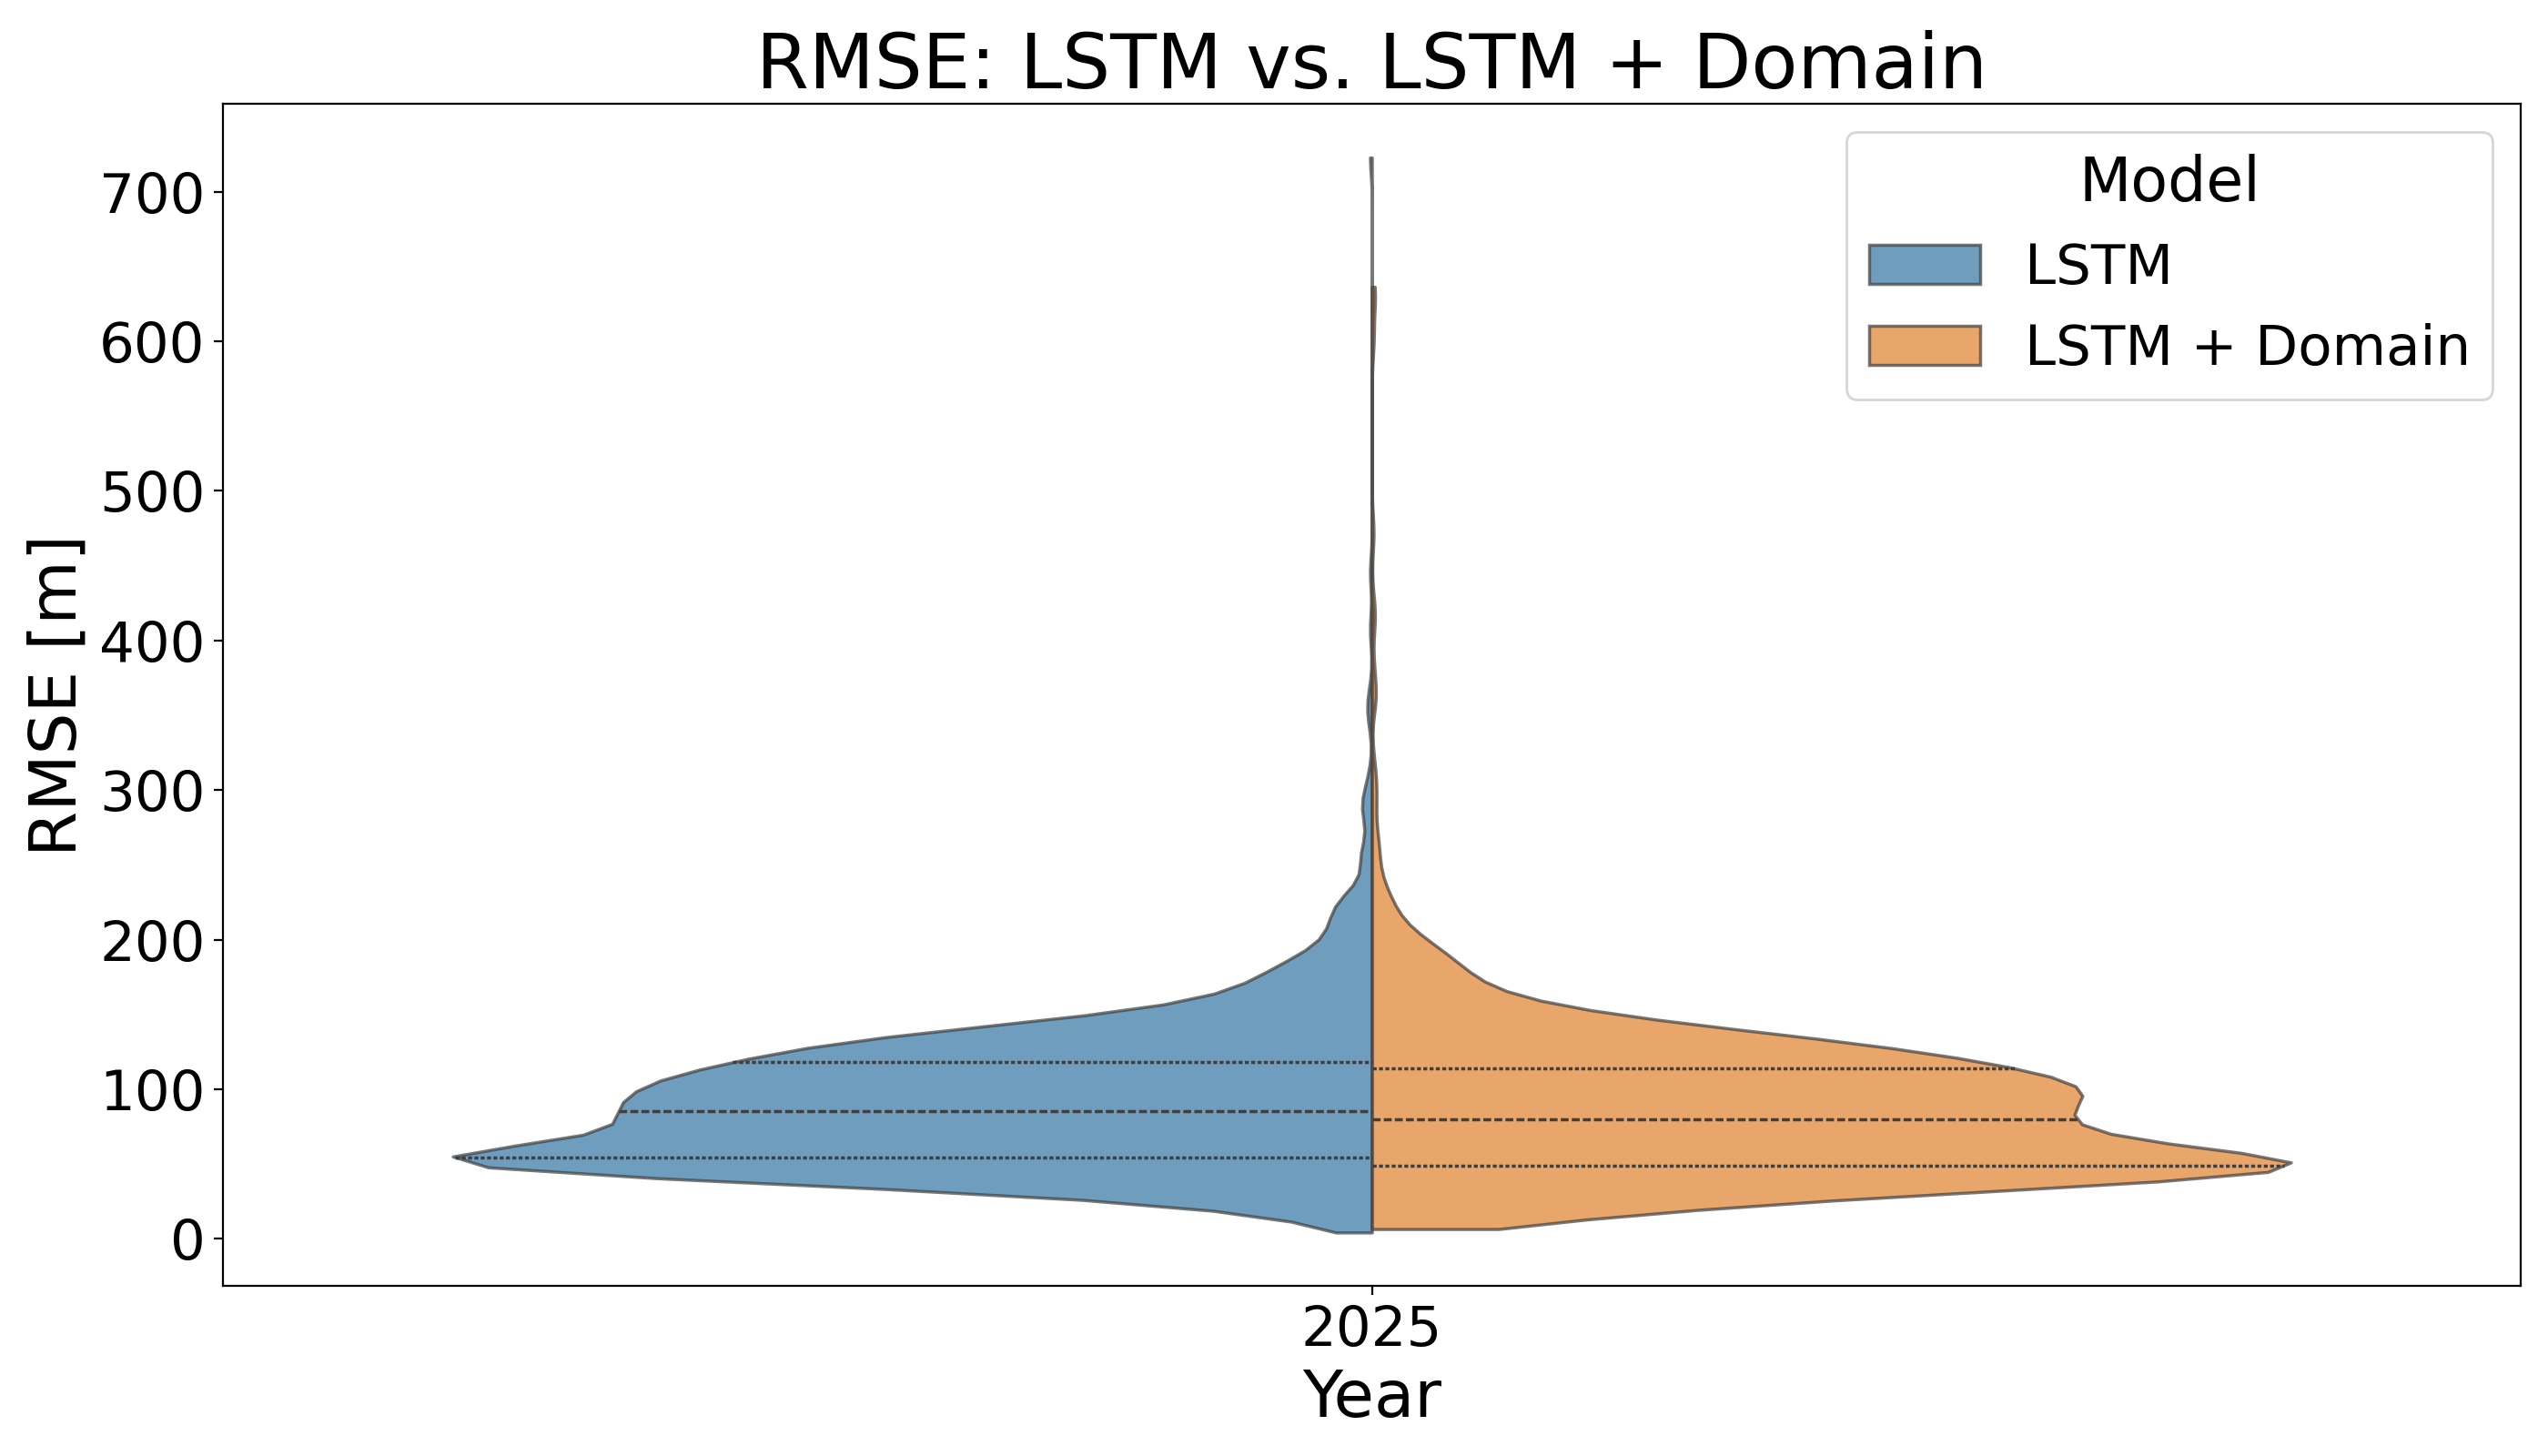
\includegraphics[width=0.7\linewidth]{figures/thesis_violin_lstm_vs_nohpo_lstm_domain_per_year.png}
    \caption[Exp. III RMSE Violin Plot]{\ac{RMSE} violin plot comparing the standard \acf{LSTM} and the \ac{LSTM} + Domain* models on the full test set.}        \label{fig:violindomaine}
\end{figure}

\begin{figure}
    \centering
    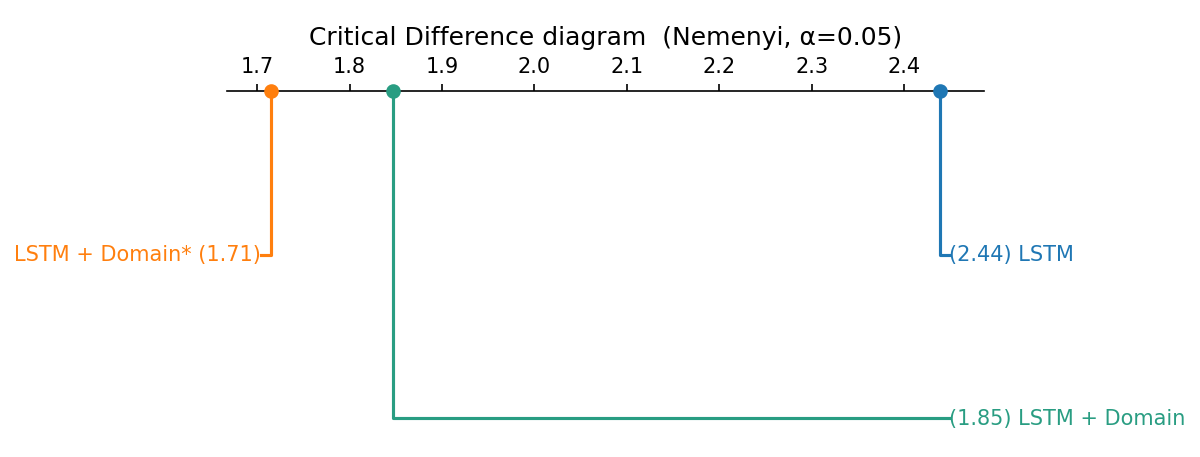
\includegraphics[width=0.7\linewidth]{figures/cd_diagram_lstm_comparison.png}
    \caption[Exp. III Friedman \& Nemenyi CD-Plot]{Critical Difference diagram comparing the \acf{LSTM} variants with and without Domain specific training.
\ac{LSTM} +Domain* refers to the \ac{LSTM} + Domain model that was run using the hyperparameters of the \ac{LSTM}
without any optimisation.}
    \label{fig:cd_exp3_real}
\end{figure}


\section*{Further Analysis}%titel anpassen


%In the preceding sections, we have shown the quantitative outcomes for each research question. 
In what follows, we discuss the mechanisms and implications behind these results, starting with a comparison of predictive capabilities across all evaluated model families, followed by an investigation of the impact of geographic domains and their encodings to model performance, and ending with a brief section on monthly trends.   

\subsection*{Predictive Capabilities of Motion Models} %was comparing. could be comparison of, but needs to be action


%\subsection{Exp. 1 Discussion}

The results provide a clear answer to the first research question: learned sequence models, particularly task-specific \acp{LSTM}, significantly outperform both classical kinematic models and stochastic filters in predicting short-term inland vessel trajectories. Following, we investigate each model family in more detail.

\paragraph{Kinematic Models.}
The performance of the kinematic models suggests that simple arc estimations are insufficient to outperform straight-line motion prediction. The \ac{CV} model learned to only use the velocity of the most recent timestep (highlighted in purple in Table~\ref{tab:hpo_results_exp0}).
This is an assumption that is also applied in most \ac{CV} definitions, which was relaxed for these experiments by parametrising context length. 
An analysis of the error distributions for the \ac{CV} and \ac{CTRV} models reveals that the resulting residuals are heavy-tailed rather than normally distributed. This deviation is reflected by low coefficient of determination ($R^2$) values of approximately 0.6138 to 0.6428 when compared against a theoretical normal distribution. Further analysis of this error distribution can be found in Figure \ref{fig:qqplot} in Appendix~\ref{chap:appendixdataplots}.
This observation leads us to a likely explanation for the optimisation result: vessel displacement over our samples could be dominated by brief, discrete regime changes rather than smooth, Gaussian drift. Averaging the displacement would therefore mix in an increasingly stale velocity estimate rather than reduce noise, so the most recent single step remains the least biased predictor of the immediate future.
With increasing model complexity, the best context size increases. The Hybrid Model learns to switch to \ac{CV} at a relatively small $\tau_\text{rot}$ of $29.28^\circ/\text{min}$. This indicates that straight-line motion is more prevalent than motion with a single arc in our dataset. 
Furthermore, Figure~\ref{fig:adepredhorizon} shows the error progression over time. While the \ac{ADE} of the \ac{CV} model does not grow perfectly linearly, it has a much more linear trend compared to the \ac{CTRV} models, which diverge heavily at longer horizons.
One cause for this difference is that the deviation of a circular arc generated by an unsuitable turn rate in \ac{CTRV} grows superlinearly with the number of prediction steps. In contrast, a wrong velocity estimate in \ac{CV} produces a constant lateral offset that accumulates linearly.
For an intuitive visual comparison of this dynamic, refer to the upper rows of Figures~\ref{fig:domain1} and \ref{fig:domain3} in Appendix~\ref{chap:appendixdataplots}.

\paragraph{Stochastic Filters.}

In the \ac{KF}, position changes are a linear function of the velocity state, so positional errors remain small as long as the velocity estimate is reasonable.
Consequently, the optimisation selected a relatively small process noise $q_\text{pos}$ compared to the measurement noise $r_\text{pos}$ (highlighted in cyan in Table~\ref{tab:hpo_results_exp0}).
The different orders of magnitude for $r_\text{pos}$ in different domains, and the respective value differences between \ac{KF} and \ac{EKF} allow us to conclude that fixing the measurement noise to values commonly found in literature would not have been sufficient.
Despite the optimised tuning, the \ac{KF} fails to surpass the simple \ac{CV} model. This points to two primary conclusions regarding its limitations.
First, the bottleneck of the prediction lies in the underlying constant-velocity assumption rather than the state estimation process itself. Second, the \ac{KF} is unsuitable for this task due to its strict reliance on Gaussian noise assumptions. In the previous section we have established that the error does not follow a Gaussian distribution.
A further methodological caveat is that the diagonal $\mathbf{Q}$ assumes uncorrelated positional and velocity noise, despite their physical coupling. The extent to which this simplification also contributes to the observed gap remains open.
Since the \ac{CV} model was optimised to only consider the last step, the Markov assumption of the \ac{KF} is not the cause for the inability of the \ac{KF} to outperform the \ac{CV} model. With the noise ratio established above and the ten correction steps available within the context window, the filter's prior is effectively forgotten by the time prediction begins, so its velocity estimate converges to the same estimate as the \ac{CV} model's last-step displacement, rather than to a genuinely smoothed estimate.

In the \ac{EKF}, position depends nonlinearly on the turn rate $\omega_k$ through trigonometric terms. This means that even a small error in the estimated rotation propagates into a drastically larger positional error over time.
The optimisation process adapted to this instability by selecting a substantially larger process noise $q_\text{pos}$ and a near-zero $q_\text{rot}$ (highlighted in green in Table~\ref{tab:hpo_results_exp0}), which indicates that the filter learned position predictions are highly unreliable when rotation is involved.
$\omega_0$ is initialised to $0$, and the minimum context length to $n_\text{ctx} = 2$.
Together, these parameters effectively restrict the underlying \ac{CTRV} model to straight-line motion with negligible curvature to avoid compounding nonlinear errors. Despite this, the \ac{EKF} outperforms the \ac{KF} significantly (Figure~\ref{fig:cd_test}). 
However, this performance gap must be interpreted with caution. Although both filters belong to the same family, their predefined search spaces differed: the context window length ($n_\text{ctx}$) was treated as an optimisable hyperparameter for the \ac{EKF} (converging to $2$), whereas it was kept fixed at the full ten steps for the standard \ac{KF}. Given that the baseline \ac{CV} model also performed best using only the single most recent step, forcing the \ac{KF} to smooth over the entire 10-step context window likely disadvantaged it. Consequently, the observed gap might partially stem from this discrepancy in the search space design rather than purely from the ability of the \ac{EKF} to handle nonlinear kinematics. Future evaluations must align the search spaces to allow for a fair comparison.
Nevertheless, looking at the error distributions, the \ac{EKF} still manages to suppress extreme outliers slightly better than the standard \ac{KF}, which is reflected in the more pronounced gap in the \ac{RMSE} metric. Since \ac{RMSE} heavily penalises large deviations, this difference demonstrates that the state estimation of the \ac{EKF} still manages to suppress extreme outliers slightly better than the standard \ac{KF}.
However, the violin plots in Figure~\ref{fig:violince} confirm that while the \ac{EKF} error distribution is shifted towards slightly lower values compared to \ac{CV} and TiRex, it still has a similar spread and long upper tails.
Therefore, while the \ac{EKF} provides a measurable baseline improvement, its fundamental handling of sudden manoeuvres and outliers is not drastically improved, consistent with the still prevailing non-Gaussian error distribution.


\paragraph{Foundation Models.}
TiRex runs best with a context length of 1. The model does not implement any attention mechanisms to selectively weight individual timestamps and has no mechanism to filter out the added noise from a longer context. It is thus prone to the same bias as the \ac{CV} model, leading to the present configuration.
With only a single input point and no learned domain adaptation, TiRex has little basis to do more than propagate it forward, which is consistent with the statistical indifference between TiRex and \ac{CV} across all point-forecast metrics.
Not only the performance, but also the generated trajectories are similar to those of the \ac{CV} models (Figures~\ref{fig:domain1}, \ref{fig:domain2}, \ref{fig:domain3}, and \ref{fig:domain4} in Appendix~\ref{chap:appendixdataplots}), indicating the foundation model predicts straight-line kinematics.
A distributional comparison of per-sample \ac{RMSE} (Figure~\ref{fig:violince}) reveals that \ac{CV} and TiRex have nearly identical violin shapes with similar medians, interquartile ranges, and tail behaviour. They confirm that TiRex effectively learns \ac{CV} kinematics without any domain-specific training.

If we consider Table~\ref{tab:results_exp0_foundation_prob}, we notice that TiRex produces extremely narrow prediction intervals compared to Chronos-2. Narrow intervals can indicate either high accuracy or poor calibration. Inspecting the coverage reveals the latter: only $5.9\%$ of true future positions fall within the nominal $80\%$ prediction intervals of TiRex, far below the ideal coverage of $0.80$.
Chronos-2, by contrast, achieves a near-ideal coverage of $0.769$.
The Winkler score of TiRex is lower than that of Chronos-2 because the score rewards narrow intervals when they happen to contain the true value, and penalises misses in proportion to interval width.
Since the intervals of TiRex are so narrow, each miss only causes a small absolute penalty.
It follows that if we want to use a foundation model and also have an accurate quantification of uncertainty, TiRex is unsuitable despite its better performance in ADE and FDE.


\paragraph{LSTM.}

The \acp{LSTM} show the strongest forecasting performance among all evaluated models by a large margin (Table~\ref{tab:results_exp0} and Figure~\ref{fig:adepredhorizon}).
Compared to the kinematics based models, they reduce the prediction error substantially.
This outperformance grows heavily as the prediction horizon extends.
This widening gap is expected: kinematic filters extrapolate purely from the last observed state without any memory of prior context, so their assumptions become increasingly inaccurate the further ahead they are extrapolated.
The \acp{LSTM}, in contrast, have access to the full context window, which allows them to remain comparatively accurate even at longer horizons within the tested window.

A visual inspection of the generated trajectories (Figures~\ref{fig:domain1}, \ref{fig:domain2}, \ref{fig:domain3}, and \ref{fig:domain4} in Appendix~\ref{chap:appendixdataplots}) explains another key advantage: the \acp{LSTM} particularly excel at estimating the correct velocity during acceleration and deceleration phases.
This capability makes the biggest difference in the lock domain, where most samples include abrupt speed changes to either start or stop vessel movement.
Overall, the network learns motion patterns that generalise far better than the handcrafted assumptions encoded in \ac{CV}, \ac{CTRV}, and the stochastic filters.
The \ac{RMSE} violin plots in Figure~\ref{fig:violince} support this, showing that the error distribution of the \ac{LSTM} is shifted toward lower values than all other models.
The network performs better on the vast majority of trajectories, while a smaller number of difficult cases still produce comparatively high errors.
The \ac{LSTM} therefore achieves not only better average accuracy but also a more favourable distribution of prediction errors.
To achieve this performance, the training process relied on the \ac{HPO} framework.
%Figure~\ref{fig:succhalfing} visualises the successive halving process during this optimisation.
%As designed, the algorithm discards several poor configurations early to save computational resources, while better trials survive longer and undergo further refinement.
%A few weak trials still run for a comparatively long time solely because the initial 26 evaluations were intentionally excluded from pruning to establish a baseline search space.

Beyond the pruning strategy, the hyperparameter importance analysis demonstrates that the input feature set is the most influential parameter for model success. Details about hyperparameter importances can be found in Figure \ref{fig:lstmhpimportances} in Appendix~\ref{chap:appendixdataplots}. 
In contrast, the analysis shows that the hidden size of the network has almost no impact on the final performance.
This indicates that the bottleneck for this forecasting task lies primarily in the provided data representation rather than the overall capacity of the model.
Interestingly, the best configuration does not use the full feature set but excludes \texttt{rot} (orange highlights in Table \ref{tab:hpo_results_exp0}).
While one might expect that adding more input features should always improve performance, as we can confirm for all other values by looking at the gradient, this result indicates that \ac{ROT} does not contribute useful information in this setting.
This is consistent with the \ac{EKF} results and suggests that the \texttt{\ac{ROT}} feature we derived is either noisy or only weakly informative for the motion patterns considered here.
Future work should revisit our choice to derive this feature manually and consider using the \textit{heading} field instead.
A deeper comparison between this plain \ac{LSTM} and a domain-aware variant follows in Exp~\Romannum{3}. % (\ref{sec:exp3}). %link kapoutt?

Figure~\ref{fig:cd_test} provides an overall summary comparison of the evaluated model families.
From this perspective, learned motion models are clearly best suited to capture the non-trivial vessel dynamics in the evaluated AIS data.
At the same time, the results show that stochastic filters remain competitive and can outperform foundation models when the underlying motion assumptions match the task reasonably well.
In contrast, increasing kinematic complexity alone does not necessarily improve performance, as the CTRV variants consistently remain among the weakest approaches.







%\subsection{Exp 2 Discussion} %neuer titel, wip alles hier 
\subsection*{The Impact of the Geographic Domain} %\me{dont like the title yet}
\paragraph{Domain Comparison.} %personally i would prefer to set \\ between some of  these statements because they are unrelated
The evaluation across different waterway types demonstrates that domains are not equivalent in terms of difficulty.
They all represent distinct motion patterns and uncertainty characteristics.
While a detailed analysis of parameter variations is beyond our scope, extreme deviations such as the \ac{EKF} learning to heavily distrust incoming positional measurements to compensate for noise serve as concrete evidence. %for those mentioned Uncertainty characteristics
The highly distinct hyperparameter configuration of the lock domain is consistent with the expectation that the data augmentation applied exclusively to this class alters the effective training distribution. 
Future work should investigate whether sampling and data augmentation should be applied more uniformly across all classes to reduce such asymmetries. %\\ todo remove empty line if this realy costs us an extrapage

The low errors observed in the channel domain suggest a homogeneous data distribution.
By contrast, the comparative difficulty of predicting the harbour domain likely reflects a more diverse set of manoeuvres, with a % denser traffic, and a
broader range of trajectory patterns.
This is consistent with the open navigable space available in harbour areas compared to the strictly confined boundaries of the other classes (Figure~\ref{fig:osm_assigned_kiel}).
Furthermore, the massive performance leap observed in the lock and channel domains when transitioning from classical models to learned architectures has clear physical causes.
The classical \ac{CTRV} and \ac{CV} models fail to estimate combinations of consecutive corners, typical for navigating channels. This dynamic could be learned by the \ac{LSTM}.
Similarly, the performance leap in the lock domain is physically driven by start-and-stop accelerations that the motion equations cannot represent.



\paragraph{Comparison to Mixed Training.}
As the results indicate, the benefit of per-domain training increases with model complexity. This varying benefit of per-domain training shows that high-capacity models are sensitive to domain heterogeneity.
They either require explicit domain conditioning or separate, domain-specific models to fully realise their potential.
The lack of statistical significance in the performance drop of the harbour domain is most likely due to the similarity of the mixed and harbour dataset distributions, with the harbour domain dominating the dataset (Table %\ref{fig:barplotaftereaugmentation}
\ref{tab:trajectory_distribution}). 
Isolating the harbour data actively degrades the performance of the \ac{EKF}.
This anomaly likely occurs because the pure harbour environment contains a higher density of %extreme 
outliers, which violates the Gaussian noise assumptions of the filter even more %severely
than the mixed dataset. %\\
The fact that the channel and lock domains benefit heavily from specialised models indicates that they represent the most distinct motion regimes within the overall dataset.
Meanwhile, the strict separation of harbour and river data is less critical for model performance in this specific setup.
When extending the model architecture to future waterways, this varying sensitivity suggests that new training domains should be defined by discovering naturally distinct motion regimes within the data. 
%These findings confirm that domain-specific training is indeed critical for high-capacity models, thus answering the second research question.
These findings support the hypothesis that domain-specific training benefits high-capacity models, addressing the second research question, albeit under the limitations discussed in chapter \ref{paragraph:comparability}.




\subsection*{Advantages of Explicit Domain Encoding} 

Interestingly, the LSTM + Domain* model that reuses the hyperparameters of the baseline LSTM outperforms the LSTM + Domain model that was tuned in a separate Optuna study with statistical significance (Figure \ref{fig:cd_exp3_real}). %\ref{fig:cd_exp3}).
During the hyperparameter search for the standard LSTM + Domain model, the optimisation algorithm failed to find a better configuration than the initial 16 trials before early stopping terminated the study.
This indicates that the search likely stopped prematurely and that the domain-aware architecture could benefit from a more exhaustive tuning procedure.
Future work should revisit this experiment with increased patience or a larger hyperparameter optimisation budget to fully exploit the potential of the explicit domain encoding.

The consistent outperformance of the LSTM + Domain models against the standard \acp{LSTM} in Table \ref{tab:results_exp3} and Figure \ref{fig:violindomaine} indicates a clear and robust dominance of the domain-aware model over the baseline.
These results provide strong evidence that explicitly encoding domain information into the model architecture consistently improves trajectory prediction performance in all considered domains.
The domain-aware model has a lower median error and lower first and third quartiles, indicating consistently better typical performance. The interquartile ranges of both models are comparable, but the baseline \ac{LSTM} shows more extreme outliers. This suggests that the embeddings help in avoiding occasional large errors. Eliminating these outliers is exactly the primary objective when deploying trajectory forecasting models in safety-critical environments.
While the best-case \acs{RMSE} of the baseline is slightly lower in this particular run, this effect was not consistent across the additional ten training runs and does not affect the overall dominance of the domain-aware model. 

We have thus answered the third research question and confirmed the impact of explicit domain encoding.
It should be highlighted that this experiment used a relatively naive domain encoding strategy across only a small number of distinct classes. Even more substantial performance improvements can be expected in future work by exploring more sophisticated encoding techniques or incorporating a broader variety of waterway environments. % conclusion?

\subsection*{Monthly Trends} 

%\paragraph{Overall Trends.} 
The monthly trends in Figure~\ref{fig:monthlytrends-all} are consistent across all models, which suggests that they are not caused by the underlying motion models, but rather reflect properties of the dataset itself.
Without data from multiple years, we cannot determine whether this constitutes a seasonal trend. Possible causes could be, but are not limited to: large vessels being easier to predict and being more represented in summer, or different traffic characteristics resulting in more evasive manoeuvres in winter.
The simplest explanation is higher data availability in the summer months combined with hyperparameter optimisation and model training being fitted to those months.
However, this does not explain why the same trend is visible for Chronos-2, which was neither trained nor tuned on this data.
We therefore take this simply as a confirmation that using a full year of data was the right decision, and note that the evaluation timeframe has a significant impact on reported results. Future work should investigate this further by incorporating older data.

%3rd version, was asked to restructure again
%





%´´´´´´´´´´´´´´´NOW COVERED IN 07´´´´´´´´´´´´´´´´´´´´´´´´´´

%!!!!!!!!!!!!!!!!!!!!!!!!!!!!!!!!!!!!!!!!!!!!!!!!!!!!!!!!




































%!TEX root=../main.tex
\chapter{Limitation \& Future Work}%todo change title to match contents
\label{chap:limitation}
\acresetall %reset abbrevations

\begin{comment}

%tim aus meeting:
%ausblick wohin? Kapitel Limitations und Future Work
%nur die sationen, nur 1 jahe.. alle annahmen. 
%transformer..
%domänenanalyse machen, wie unterschiedlich die sind
%feature weights (abaltio bei auswertung oder mischen) pro modell -> wo ist was am wichtigsten? dadurch fazit domäne relevant
%domnenentscheidung datanbasiert, evtl statdesse nclustern etc
%vq transformer
%augmentation




\end{comment}
\todo{limitation schiff muss wissen wo es ist -> OSM interface muss bestehen; außerdem mögliche analyse wie viel data hilft wirklich, wie schnell kovergiert es wenn man sampled kann massiv zeit sparen; außerdem, consider waterboundaries if we use osm dataa anyways}

%\todo{manual sampling before running the TPE-> biased to that region, lack of exploitation-> either also add more random runs, or do HP selection befroehand, or just add many random runs that will cover all hp sets. at least the initial runs were very likely globally good, as i optimised them on a smaller set, so this can also be seen as a prior we want to bias to, though that was not my intention}

\ws{This chapter can be a section* in the conclusions chapter. No need to give it a separate chapter.}
\todo{ 
There are also notes regarding the combination of Chapters 7, 8, 9 in one. 
    I can only read these after the restructuring. Now, it won't be as effective to read the text out of correct context.
}\\
\section{Dataset limitations}

\paragraph{Dataset Coverage and AIS Biases.}
The results in this thesis are based on AIS logs from three German measurement stations and a single calendar year. While the datasets cover a large number of trajectories, they still reflect the traffic patterns of a limited set of waterways and regulatory conditions. For the observation period of the year 2025, the data availability varies across the three measurement sites: Kiel (357 days), Wedel (351 days), and Bremerhaven (326 days). In AIS networks,  data loss can occur for diverse reasons, such as hardware maintenance. Notably, there were no data for June 2025 in Bremerhaven. The gaps are not a concern in practice. Since the deep learning models operate on short, localised trajectory windows rather than continuous long-term sequences, full calendar coverage is not required. Each available day yields a large number of independent training samples, and together they cover a representative variety of traffic pattern. Extending the analysis to additional years and measurement sites systems would be necessary to assess whether the observed error distributions and monthly trends generalise well. 

Furthermore, the data primarily reflects the movement patterns of large commercial vessels, which are mandated to carry Class A transponders under the \ac{SOLAS} \parencite{solas2014}. This includes cargo vessels exceeding 300GT on international voyages and all tankers. Consequently, smaller recreational craft and fishing vessels with Class B transponders are significantly underrepresented. Because Class B devices transmit at lower power and with less frequent update rates (as detailed in Table \ref{tab:ais-frequencies}), the resulting models may be biased to the more predictable dynamics of large commercial ships.

\paragraph{Augmentation and class imbalance.}
The geometric augmentation detailed in Section \ref{subsubsec:augmentation} addresses the class imbalance for lock manoeuvres, but it also introduces specific assumptions into the training data. 
The spatial coordinates ($x, y$) and angles are transformed, but the temporal spacing ($\Delta t$) and the velocity magnitude (\ac{SOG}) remain unchanged. Thus, the model observes the exact same acceleration and deceleration patterns multiple times, only from different directions. This repetition increases the risk of the model memorizing specific kinematic profiles rather than learning generalised lock approach behaviour and potentially elevates the epistemic uncertainty when the model encounters new velocity profiles during inference.\\
Additionally, random rotation assumes spatial invariance, implicitly treating the vessel motion as independent of environmental directionality. For locks, this assumption can safely be made, but one should be careful when augmenting e.g. rivers, where local currents, or wind conditions influence manoeuvring dynamics.\\
Similarly, the mirroring operation assumes perfect lateral kinematic symmetry, neglecting real-world asymmetries such as the propeller walk , which is common in single-screw inland vessels at low speeds. While these simplifications are necessary to generate a balanced dataset, they limit the exposure of the model to direction-specific environmental disturbances.

Because only data within the lock domain were augmented, hyperparameters are distinct and hard to compare to the other domains. Future work should explore alternative strategies for handling rare domains, such as downsampling of other classes, and quantify how strongly these design choices affect the error distribution and the robustness of the models


\paragraph{Derived kinematic features.}
\label{subsubsec:kinematiclowvel}
A notable limitation in the data preprocessing pipeline stems from the fact that the \ac{ROT} is not directly available in most raw AIS messages. It was derived analytically as the time derivative of the \ac{COG}. Since \ac{COG} is calculated from consecutive \ac{GNSS} position fixes rather than being measured by a dedicated directional sensor, it can become highly unreliable at near-stationary speeds. At low velocities, the localisation noise of the \ac{GNSS} receiver exceeds the actual distance travelled. This causes the computed \ac{COG} vector to fluctuate, resulting in artificial, physically unrealistic ROT spikes that do not reflect actual vessel movement. 

While the true heading channel of the vessel offers a more stable orientation metric at low speeds, we do not use it as as an alternative feature for two primary reasons. First, as per \textcite{itu-r-m1371-1-2001}, true heading is an optional AIS field and is frequently missing, particularly among smaller inland vessels equipped with Class B transponders. Second, heading only indicates the direction the bow of the vessel is pointing, whereas \ac{COG} represents the actual path of motion over the earth. Because inland waterway vessels can be subjected to lateral drift from river currents and wind, \ac{COG} was used for predictions, despite the % \ac{GNSS}-induced 
limitations at near-zero velocities. %unterschied COG und true heading wäre interessant für den schwimmwinkel als indikator für strömunbg. geht hier aber zu weit und nur möglich wenn wir stark filtern da nicht oft verfügbar
Since both the EKF and the LSTM optimisation indicate that the derived rate-of-turn signal does not contribute much predictive value, this choice should be revisited in future works.










\section{Methodological limitations}


\paragraph{Hyperparameter optimisation bias.}
We initialised the Optuna search for the \ac{LSTM} with a manually selected subset of starting configurations (16 out of 26 seeding trials). This ensures that all feature sets are evaluated at least once, but it also introduces an implicit prior over the search space, because the \ac{TPE} sampler conditions its density estimates on these seedings. Future work should therefore compare this seeded strategy against a larger number of fully random initial trials or split up the search into two stages, to separate feature selection from the remaining hyperparameters, and quantify the difference to our implementation.


\paragraph{Statistical analysis.}
The statistical analysis in Chapter \ref{par:statistical} is based on file-level aggregated metrics, with one file representing one domain on one day on one measurement station. This is used as a fallback to per-trajectory evaluation, since only the aggregated errors were available at evaluation time. As a result, all files contribute equally as blocks, even though they may contain different numbers of trajectories. %If the Friedman test is significant , we apply the Nemenyi post-hoc test for pairwise comparisons and visualise the results using a critical difference diagram. 
Future iterations of this work should save the per-trajectory evaluation for more accurate metrics.


\paragraph{Domain labels and context representation.}
The work relies on a four-class domain labelling scheme (harbour, river, channel, lock) obtained from OpenStreetMap. %For trajectories with multiple domains, a majority vote is applied.
A natural next step would be to refine the domain representation, for example by introducing additional domain types, or by clustering waterway segments based on kinematic statistics to obtain a more fine-grained context. It would also be interesting to investigate whether representing the domain as a sequence over time, instead of a single static vector per sample, further improves performance for longer context windows.

\paragraph{Hyperparameter optimisation budget.}
Because of the pruning and early stopping mechanisms we used, hyperparameter search can terminate before the true optimum is explored. The observation that the domain-aware LSTM with reused hyperparameters outperforms the separately tuned variant suggests that at least one Optuna study stopped prematurely. Future iterations of this work should consider larger budgets or more conservative pruning schedules for the most promising architectures.



\section{Model-specific limitations}

\paragraph{LSTM architecture.}
The LSTM model implemented in this thesis uses a stacked encoder with a linear decoder that predicts the full horizon in a single step. This choice matches the short 5-minute prediction horizon, but it also restricts the flexibility of the architecture. Autoregressive decoders, where each predicted step is fed back into the model as additional context, are the standard for \acp{LSTM}. In the current setup, both context and prediction length are fixed and identical across all models, so it remains unclear how sensitive the observed ranking between models is to these design choices. Future work should therefore investigate autoregressive decoders and variable context and prediction windows.
Additionally, a bidirectional encoder should be investigated, as it has improved model performance in other scenarios \parencite{articlebilstmsus}. Other gains could be found by introducing attention mechanisms, that give higher weights to relevant timestamps of the context window. 
In addition to time-wise attention, covariate-informed forecasting with attention across feature channels is particularly relevant. The comparison between Chronos-2 and TiRex suggests that cross-channel attention can provide an advantage over univariate or channel-independent sequence models. At the moment, TiRex is limited to univariate inputs, and the LSTM uses only a simple concatenation of features without explicit channel weighting. Ongoing work on extending x-LSTM-based models such as TiRex to handle multivariate, covariate-informed inputs would offer a direct opportunity to revisit this comparison once such models become available. Beyond recurrent architectures, Transformer models for time series have shown promising results in other forecasting domains, mainly due to their ability to model long-range dependencies. Training such models from scratch on the AIS data was out of scope for this thesis because of the associated runtime and tuning cost, but remains an interesting direction for future work. \me{To Tim: Ich finde den sprung zu VQ transformer immer noch nicht sinnvoll und empfehle ihn hier daher nicht. Transformer haben eine längere Trainingszeit als LSTM. Der VQ Transformer wirkt dem entgegen für lange kontexte. Diese liegen hier aber nicht vor.}

\paragraph{Uncertainty quantification for learned models.}
 For applications in multi-target tracking and autonomous navigation, a well-calibrated estimate of predictive uncertainty is important. A natural extension would therefore be to equip the LSTM with probabilistic outputs%, for example by ... %predicting multiple quantiles, training small ensembles, or applying conformal prediction on top of the existing point forecasts.
 %\todo{look into it, types of uncertainty} Such methods 
 . That would make it possible to evaluate the calibration of LSTM-based motion models in the same way as for the probabilistic baselines and to study how uncertainty behaviour differs between domains.

%-------------------------------postambel
%\me{das hier runter sehr unwihtig}
%   - What worked, what didn't, why
%   - Generalisation, runtime, practical constraints
 %  - Integration considerations for IRT pipeline


  


%\section{Methodological Challenges and Data Anomalies}
%\me{eher für rückfragen as so challenges waren, aber da platz sowieso knapp ist ist das egal}
%Developing and migrating the data pipeline presented a few technical challenges that required specific workarounds. Early in the prototyping phase, while using a small, locally subsampled dataset, the model consistently achieved a lower loss on the validation set than on the training set. This unexpected behaviour was caused by an uneven class distribution within the small sample size. A standard random split of a highly diverse dataset created a validation set filled with simple, easy-to-predict trajectories. To fix this, a data stratification strategy was implemented.Once this stratification was applied to the full dataset the data distribution stabilised and the validation metrics behaved as expected. %wurde ja auch garnicht behoben

%Another critical issue occurred when moving the pipeline between different working environments. Running the code on a new machine led to a massive, drop in valid harbor trajectories. This was traced back to a version mismatch in the \textit{pandas} library. Between major versions, the default parsing resolution for \texttt{datetime} objects changed from nanoseconds to seconds. Because the spatial jump-detection filter relied on implicitly converting these timestamps to integers, the newer library version caused the code to calculate microscopic time-deltas ($\Delta t$). This math error made the filter compute physically impossible speeds, causing it to aggressively delete thousands of valid, slow-moving harbor maneuvers. The issue was resolved by rewriting the filter to explicitly calculate the time difference in seconds in order to work with all pandas version.

%A third issue emerged during the first full-dataset evaluation with the baseline model. The RMSE was several orders of magnitude larger than the ADE, indicating the presence of extreme coordinate outliers. These were traced to overshoot artefacts introduced by cubic spline interpolation during resampling: rarelz, the spline solver produced physically impossible position jumps of up to tens of kilometres after the jump filter had been applied. The interpolation method was replaced with PCHIP, which guarantees monotonicity within each interval and cannot overshoot the local value range. Additionally, the time-gap guard in the track segmentation step was tightened to reject any window whose actual elapsed time exceeded the theoretical context-plus-prediction duration, eliminating tracks with hidden data gaps that would otherwise produce misleading ground-truth positions.
%!TEX root=../main.tex
\chapter{Conclusion}%todo change title to match contents
\label{chap:conclusion}

open




%%!TEX root=../main.tex
\chapter{Acknowledgements}%todo change title to match contents
\label{chap:acknowledgements}


\ac{OSM}: $https://wiki.openstreetmap.org/wiki/Researcher_Information$ \cite{OpenStreetMap}


\printbibliography[heading=bibintoc, title=References]

\newpage
\pagestyle{empty}

\appendix % turns every chapter into new appendix(A, B,..?)

%\chapter{Supplementary Data and Plots}
%!TEX root=../main.tex
\chapter{Supplementary Figures} %unpassend
\label{chap:appendixdataplots}
%data and plots

\begin{figure}[htbp]
    \centering
    \begin{subfigure}[t]{0.54\textwidth}
        \centering
        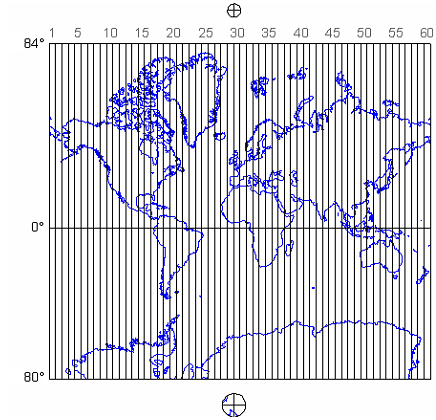
\includegraphics[width=\linewidth]{figures/ch2-fig8.png}
        \caption{Illustration of the 60 UTM zones dividing the Earth's surface, each spanning
                 6° of longitude. Polar regions beyond 84°\,N and 80°\,S are
                 excluded and covered by separate polar coordinate systems.}
        \label{fig:utm_zones_world}
    \end{subfigure}
    \hfill
    \begin{subfigure}[t]{0.42\textwidth}
        \centering
        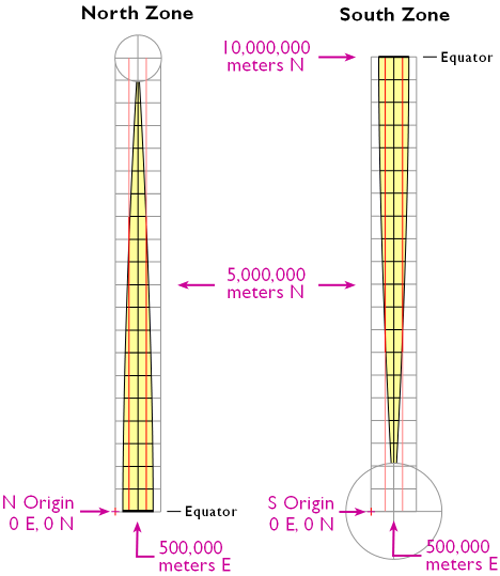
\includegraphics[width=\linewidth]{figures/UTM_Coordinate.png}
        \caption{Structure of a single UTM zone. Each zone spans 6° of
                 longitude and is subdivided into a north and south half at
                 the equator. Origins are placed 500{,}000\,m west of the
                 central meridian so that all coordinates within the zone are
                 positive.}
        \label{fig:utm_zone_detail}
    \end{subfigure}
    \caption[UTM coordinate overview]{The \ac{UTM}
             projects geographic (spherical) coordinates onto a planar
             Cartesian grid.
             Figures from \textcite{DiBiase_PennState_GEOG160},
             licensed under CC~BY-NC-SA~4.0.}
    \label{fig:utm_overview}
\end{figure}



\begin{comment}
    
\begin{figure}[htbp]
    \centering
    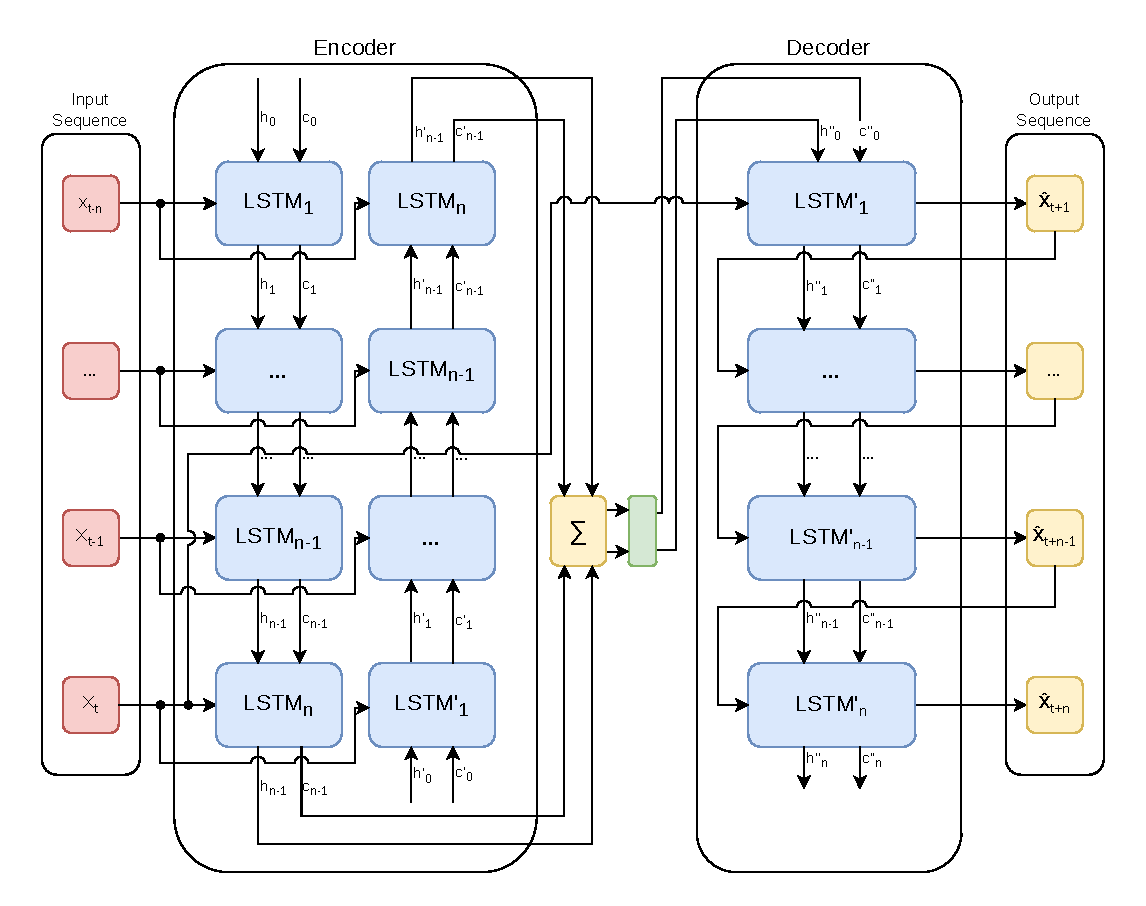
\includegraphics[width=0.75\linewidth]{figures/S2S_Bi-LSTM.drawio (1).pdf}
    \caption{Architecture utilizing a Bi-LSTM Encoder with a standard LSTM Decoder.}
    \label{fig:s2s_bilstm_appendix}
\end{figure}

\begin{figure}[htbp]
    \centering
    % \includegraphics[width=0.75\linewidth]{figures/S2S_Attention.drawio.pdf}
    \todo{wenn ich zeit für sowas habe. nachdem ich mich für architektur entschieden habe, diese hier rein}
    \caption{Sequence-to-Sequence architecture incorporating an Attention mechanism.}
    \label{fig:s2s_attention_appendix}
\end{figure}
\end{comment}







\begin{comment} %verison ohne resampling
    
% Seite 1: Folien 1–3
\begin{figure}[p]
    \centering
    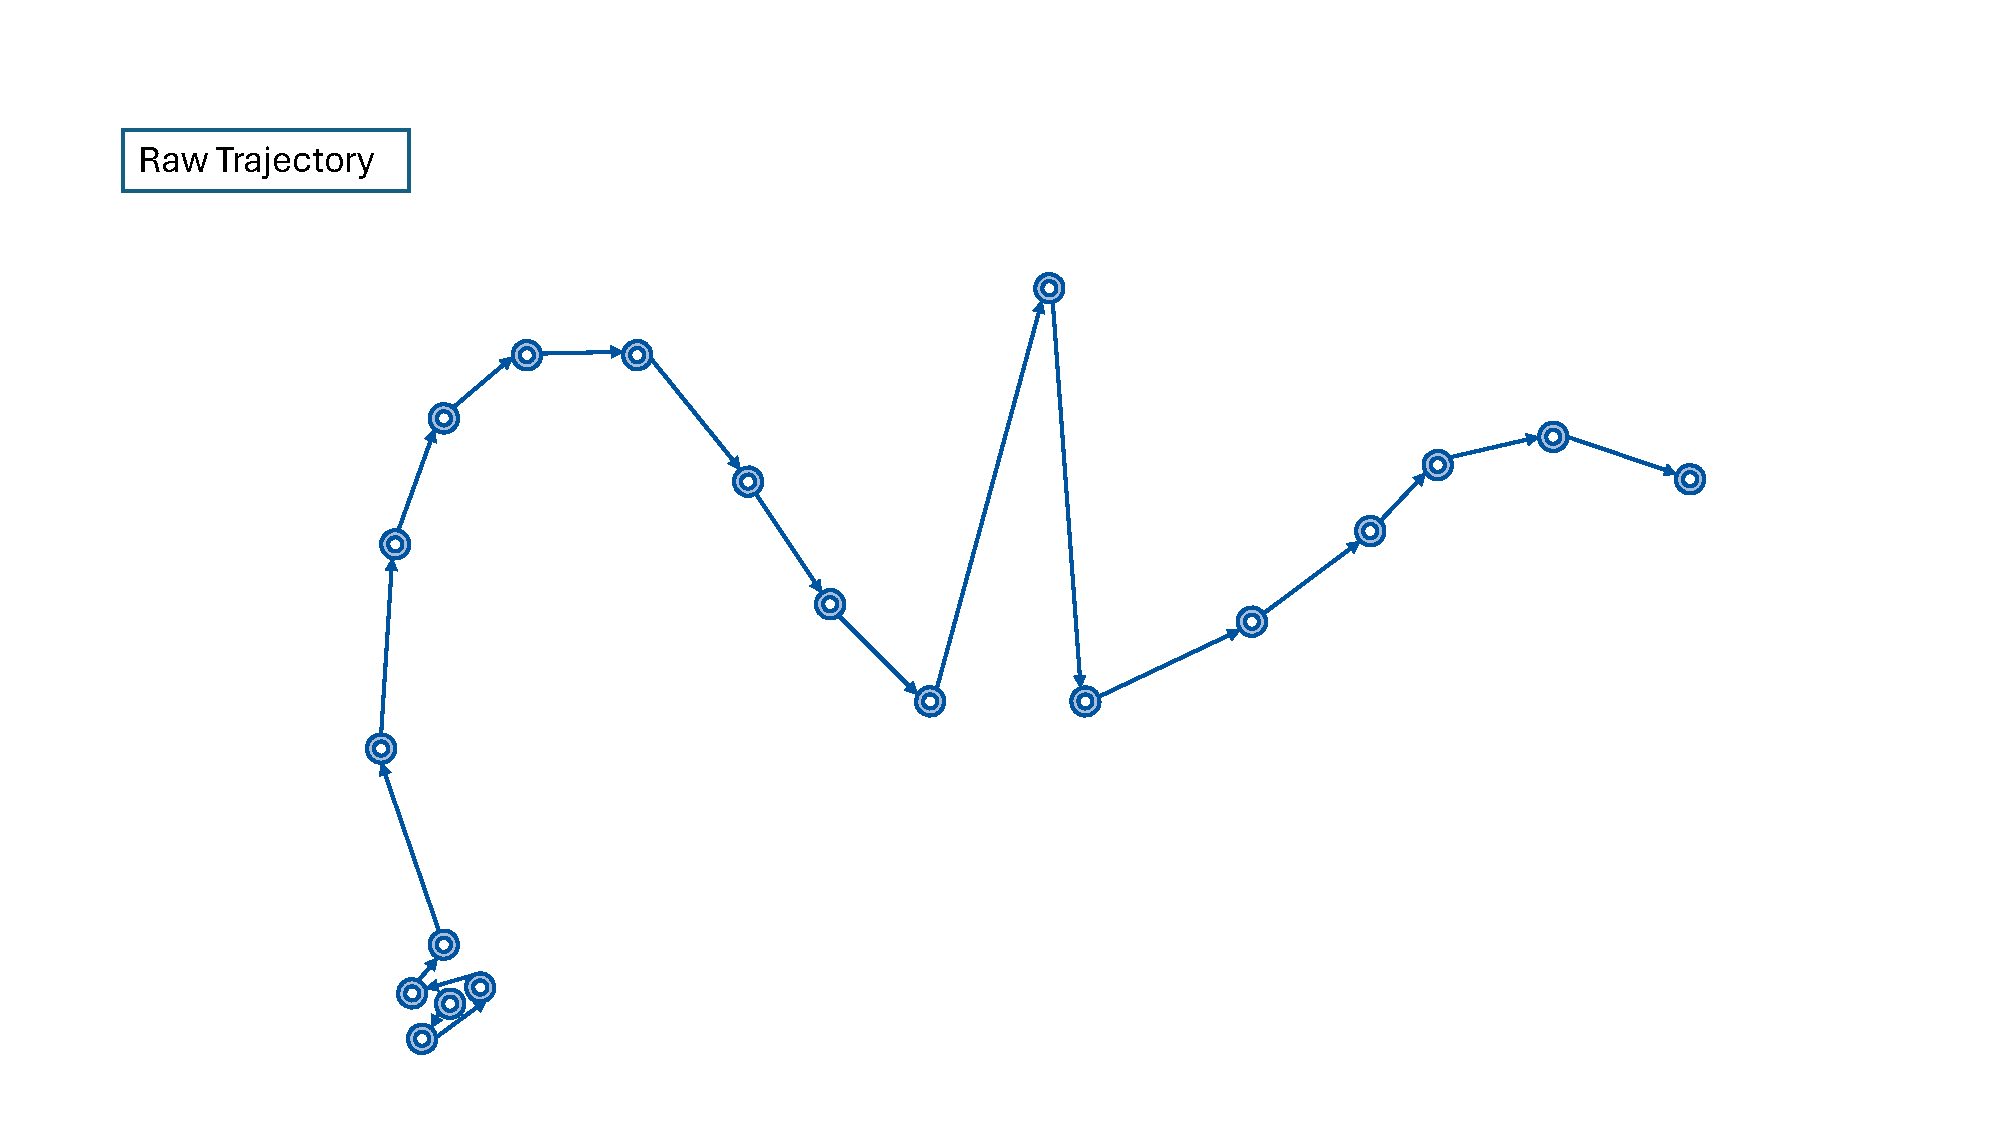
\includegraphics[height=0.32\textheight, page=1]{figures/Animation Preprocessing.pdf}\\[4pt]
    \includegraphics[height=0.32\textheight, page=2]{figures/Animation Preprocessing.pdf}\\[4pt]
    \includegraphics[height=0.32\textheight, page=3]{figures/Animation Preprocessing.pdf}
    \caption{Track Segmentation (1/2)}
    \label{fig:preprocessing-a}
\end{figure}

% Seite 2: Folien 4–5
\begin{figure}[p]
    \ContinuedFloat
    \centering
    \includegraphics[height=0.32\textheight, page=4]{figures/Animation Preprocessing.pdf}\\[4pt]
    \includegraphics[height=0.32\textheight, page=5]{figures/Animation Preprocessing.pdf}
    \caption{Track Segmentation (2/2)}
    \label{fig:preprocessing-b}
\end{figure}
%nochmla
\end{comment}

% Seite 1: Folien 1–3
\begin{figure}[p]
    \centering
    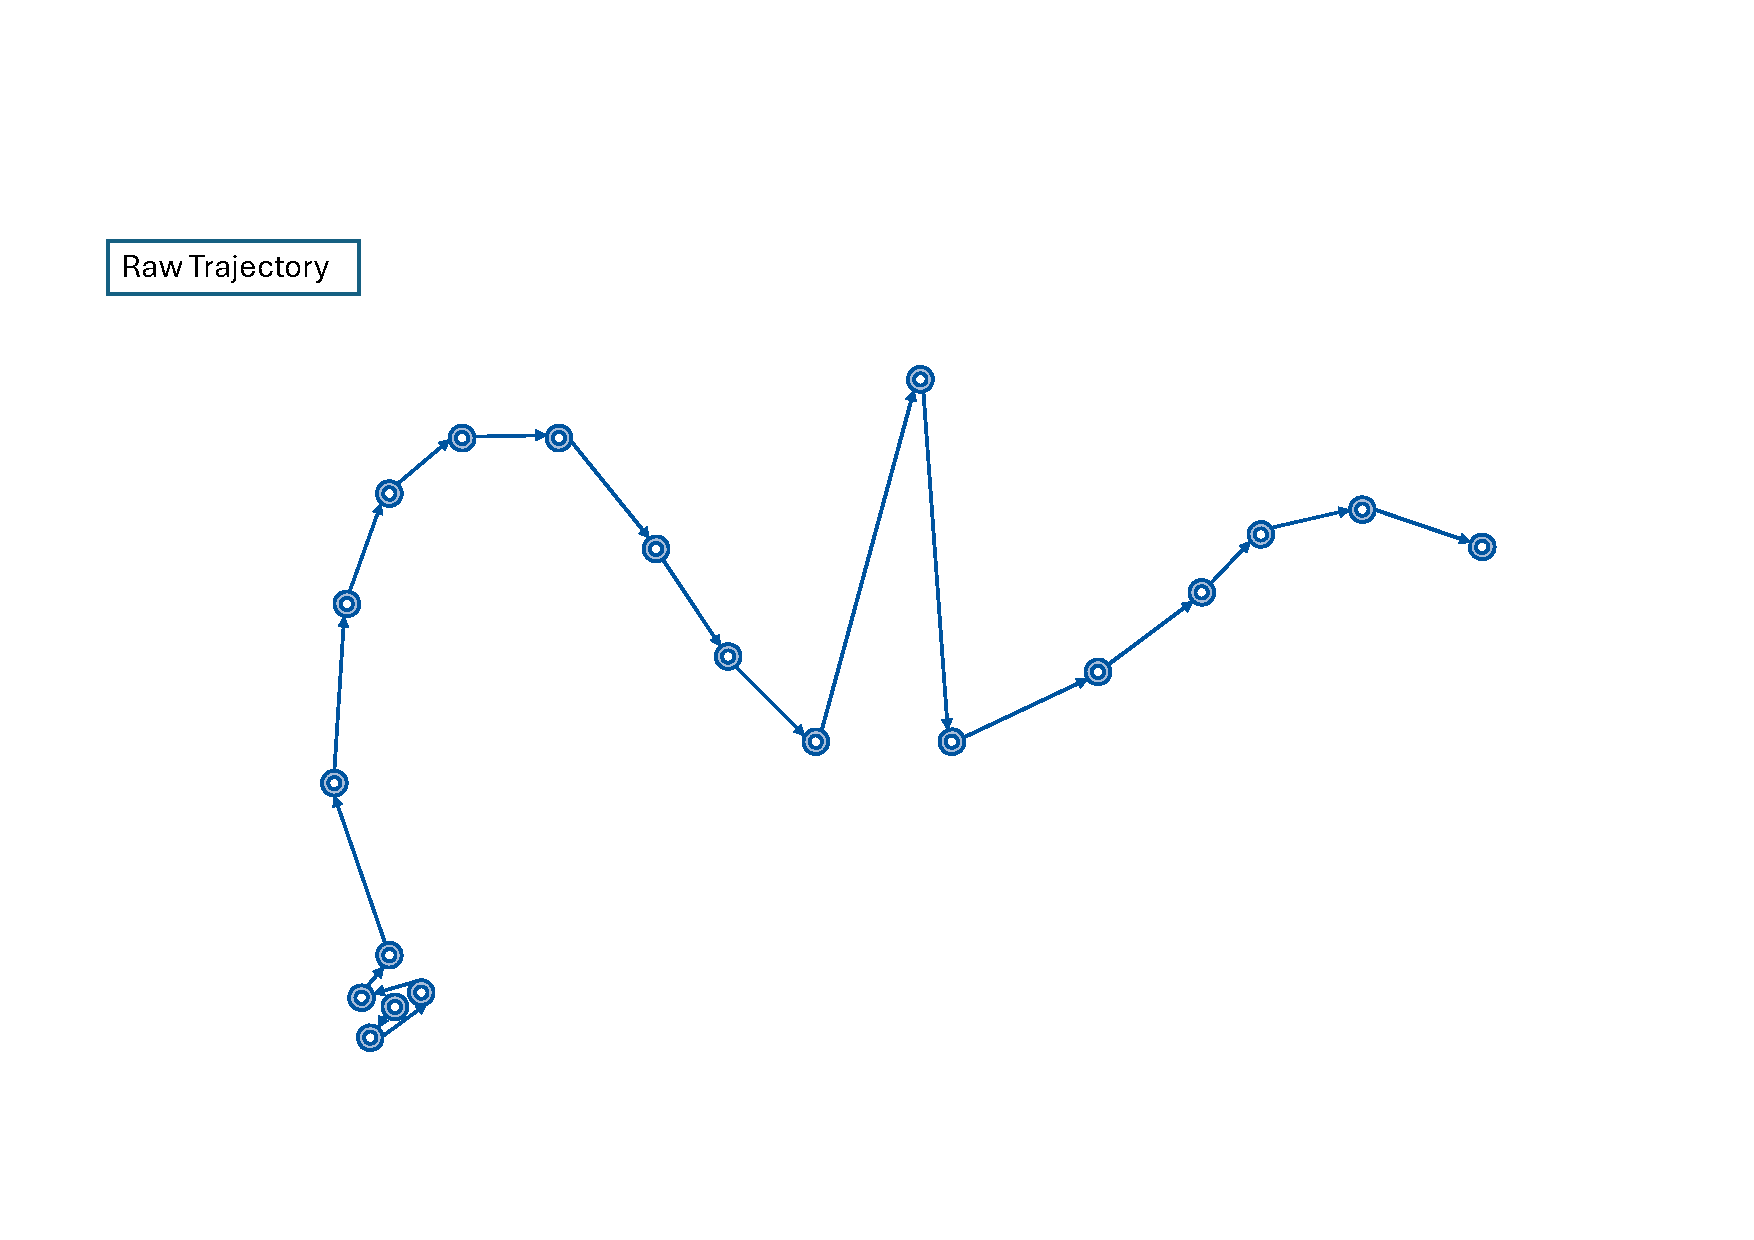
\includegraphics[height=0.32\textheight, page=1]{figures/animationpreprocessingwithsampling.pdf}\\[4pt]
    \includegraphics[height=0.32\textheight, page=2]{figures/animationpreprocessingwithsampling.pdf}\\[4pt]
    \includegraphics[height=0.32\textheight, page=3]{figures/animationpreprocessingwithsampling.pdf}
    \caption[Preprocessing visualisation (1/2)]{Preprocessing visualisation. First, implausible messages are removed. The remaining trajectories are then resampled to a fixed 30 s grid. After resampling, a sliding window is applied to extract the final samples. (1/2)}
    \label{fig:preprocessing-a}
\end{figure}

% Seite 2: Folien 4–7
\begin{figure}[p]
    \ContinuedFloat
    \centering
    \includegraphics[height=0.32\textheight, page=4]{figures/animationpreprocessingwithsampling.pdf}\\[4pt]
    \includegraphics[height=0.32\textheight, page=5]{figures/animationpreprocessingwithsampling.pdf}\\[4pt]
    \includegraphics[height=0.32\textheight, page=6]{figures/animationpreprocessingwithsampling.pdf}\\[4pt]
    %\includegraphics[height=0.32\textheight, page=7]{figures/animationpreprocessingwithsampling.pdf}\\[4pt]

    %letzt folie nicht ultra wichtig

    \caption[Preprocessing visualisation (2/2)]{Preprocessing visualisation. First, implausible messages are removed. The remaining trajectories are then resampled to a fixed 30 s grid. After resampling, a sliding window is applied to to extract the final samples. (2/2)}
    \label{fig:preprocessing-b}
\end{figure}
%nochmla



\begin{figure}[h]
    \centering
    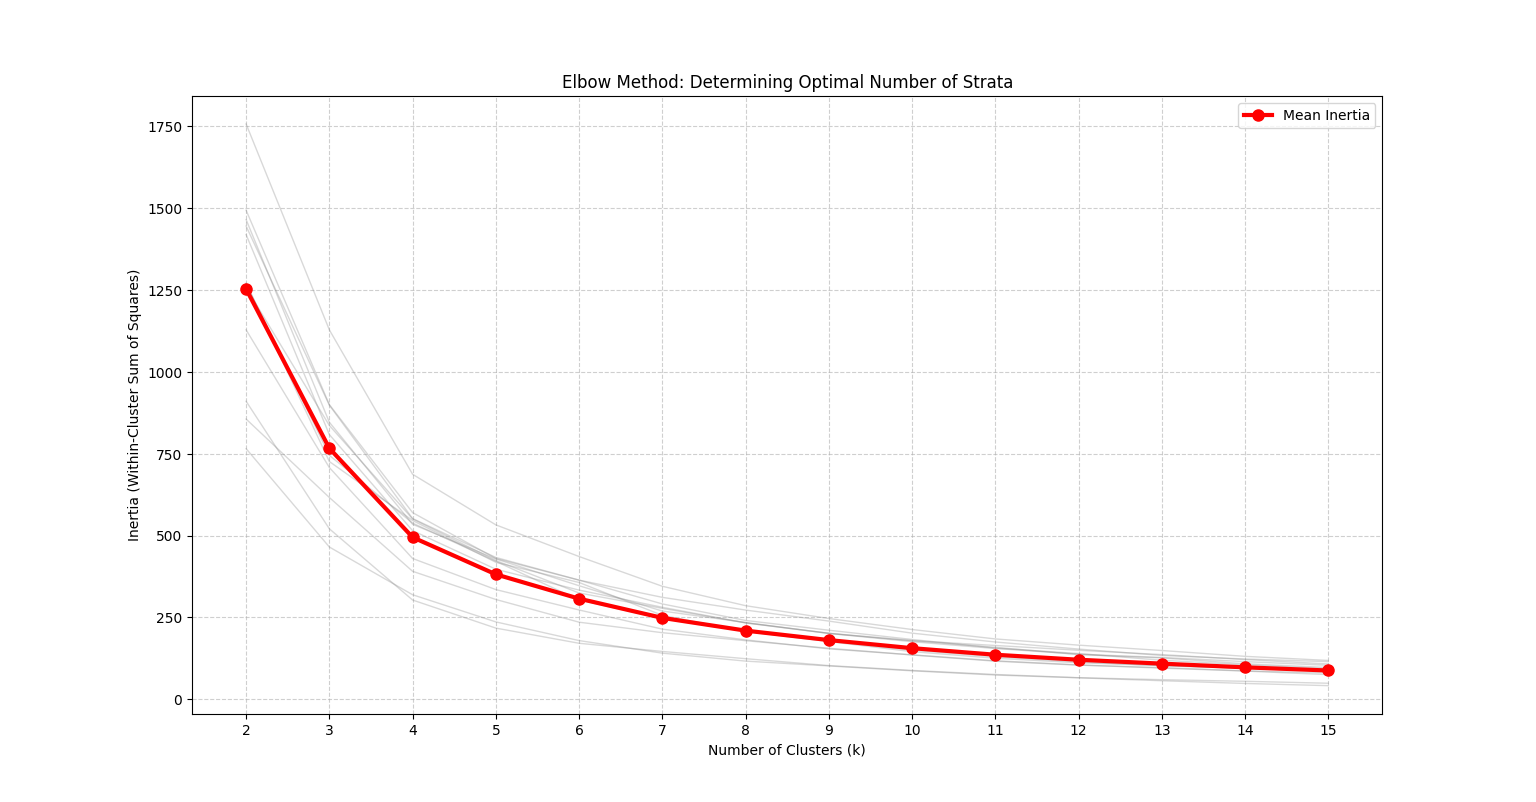
\includegraphics[width=1\linewidth,trim=0 8 0 70,clip]{figures/elbow_strat.png}
    \caption[Strata Elbow-Plot]{Elbow-Plot: Inertia vs. Number of Clusters $k \in [2, 15]$ used to estimate the optimal number of strata. For each file in the sampled dataset, vessel profiles were aggregated by computing mean \acf{SOG}, maximum absolute \acf{ROT}, and the context label. Features were standardised prior to clustering. KMeans ($n\_init=10$) was fitted independently per file; grey lines represent per-file inertia curves, the red line indicates the mean across all files. The elbow between $k=4$ and $k=5$ justifies the choice of five strata to capture the kinematic diversity of the dataset.}
    
    \label{fig:elbow_strat}
\end{figure}

\begin{comment}
\begin{figure}[h]
    \centering
    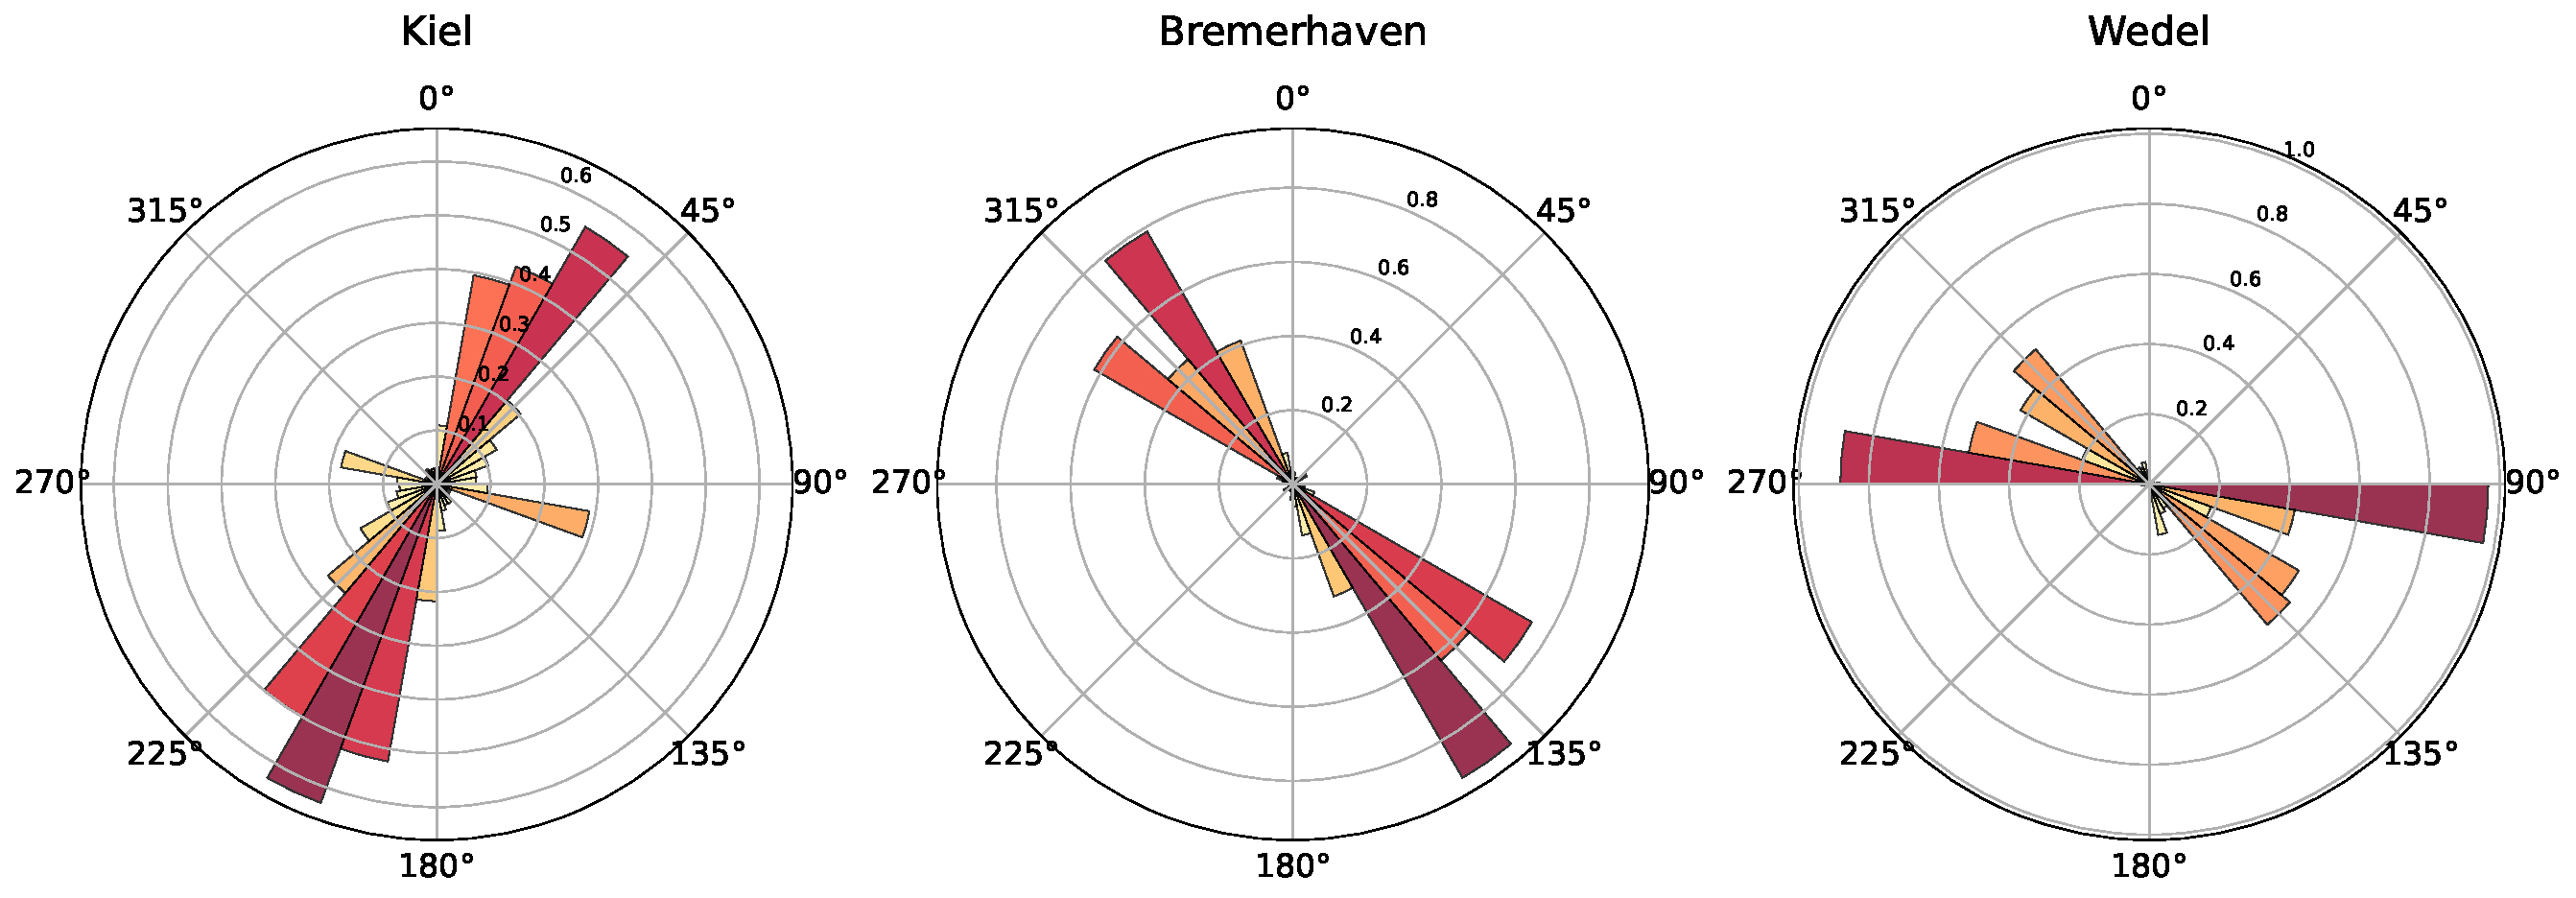
\includegraphics[width=0.85\linewidth]{figures/cog_polar_heatmap.pdf} %\todo
    \caption[COG Polar Histogram]{Polar Histogram of Vessel \acf{COG} after the Preprocessing Pipeline \todo{bigger labels orcut of the top and write Kiel left, bremerhaven middle wedel right}}
    \label{fig:polarhist}
\end{figure}
\end{comment}

\begin{figure}[h]
    \centering
    \begin{subfigure}[b]{0.95\linewidth}
        \centering
        % trim=left bottom right top. Increase the last value to cut more from the top.
        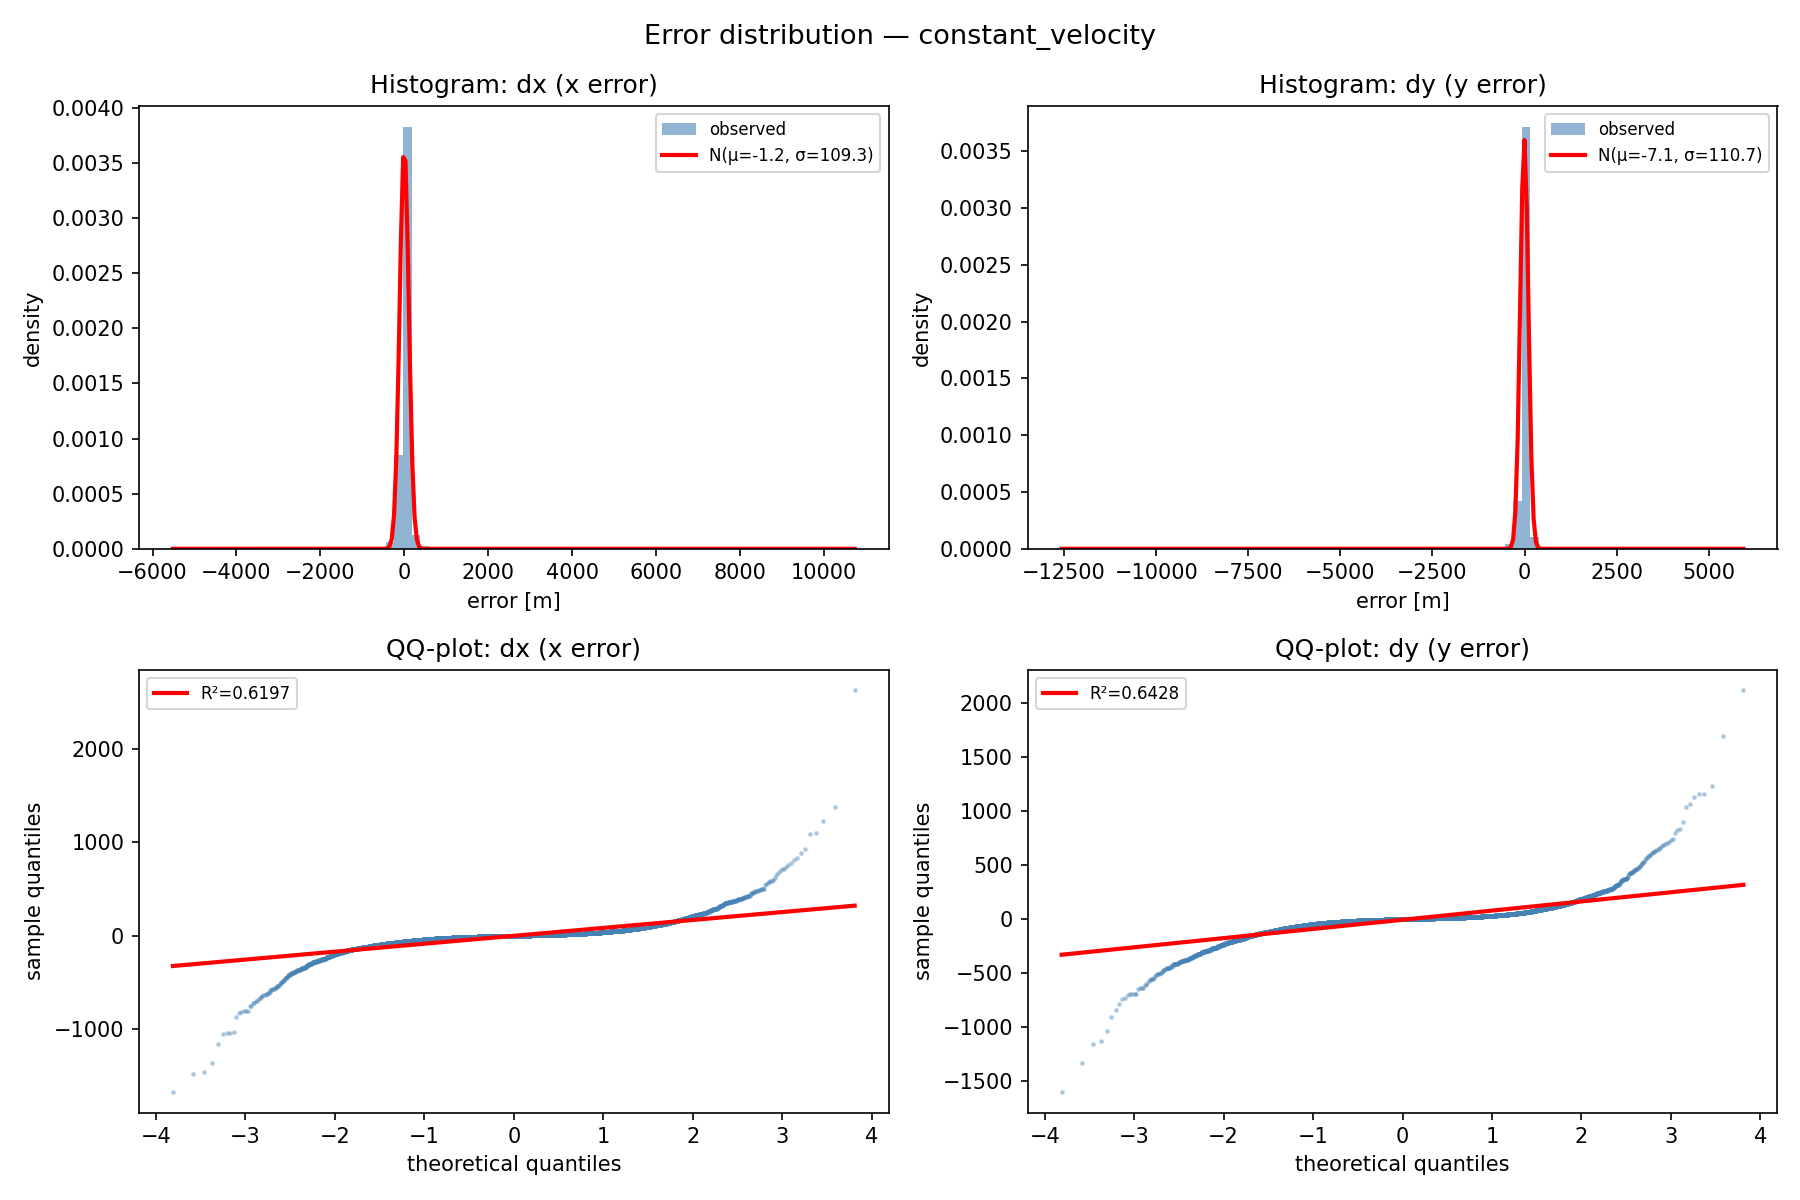
\includegraphics[width=\linewidth, trim=0cm 0cm 0cm 105mm, clip]{figures/error_distribution_constant_velocity.png}
        \caption{\acs{CV}}
        \label{fig:qqplot_cv}
    \end{subfigure}
    
    \vspace{1em} % Adds a bit of vertical space between the top and bottom plots
    
    \begin{subfigure}[b]{0.95\linewidth}
        \centering
        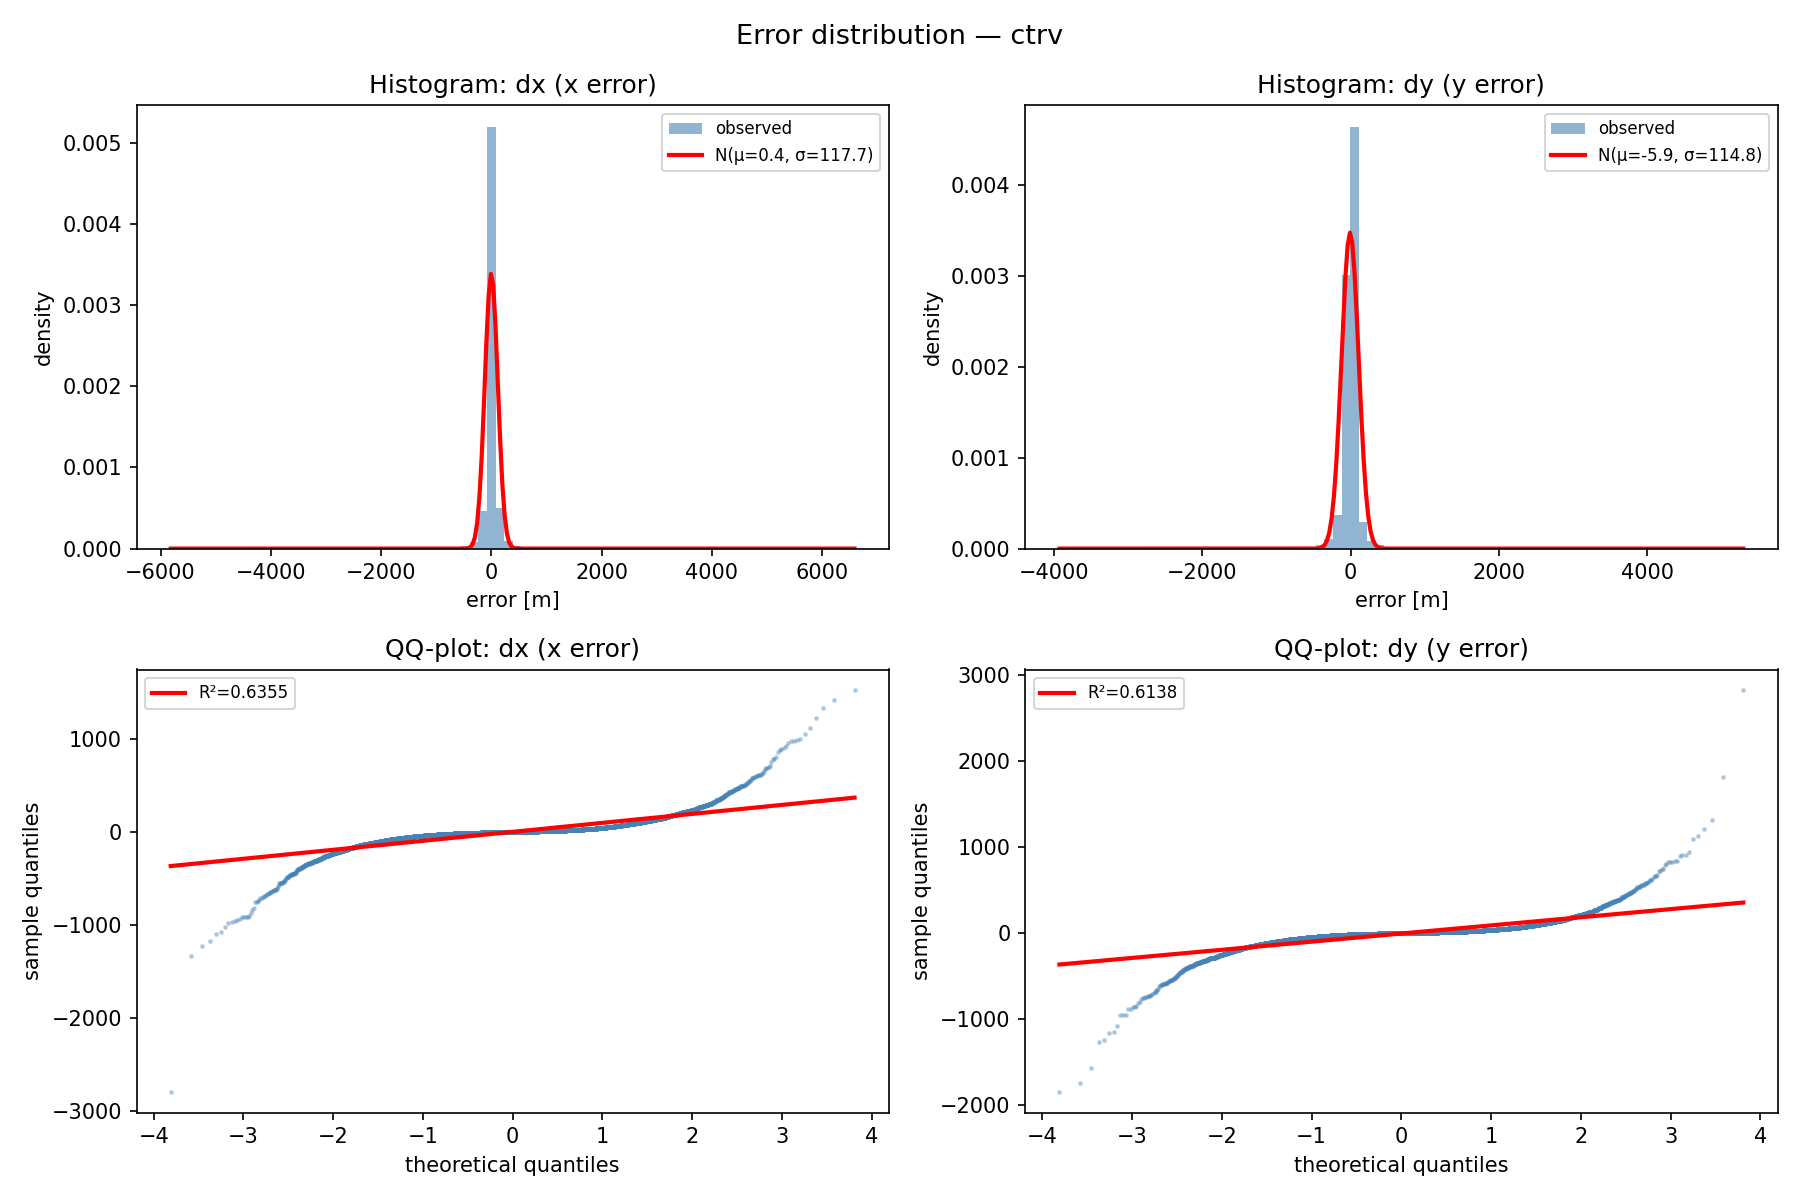
\includegraphics[width=\linewidth, trim=0cm 0cm 0cm 105mm, clip]{figures/error_distribution_ctrv.png}
        \caption{\acs{CTRV}}
        \label{fig:qqplot_ctrv}
    \end{subfigure}
    
    \caption[CV and CTRV QQ-Plot]{    
    Quantile-Quantile (QQ) plots of the positional prediction errors ($dx$ and $dy$) for \acf{CV} and \acf{CTRV} models. The errors of these pure kinematic models represent the real process noise of the \acp{KF}' underlying motion models, %plural
    which they internally model as a Gaussian distribution. The solid red lines represent the theoretical normal distribution; the significant deviation of the sample quantiles at the extremes indicates heavy tails and extreme outliers. This is supported by low coefficient of determination ($R^2$) values ranging from 0.6138 to 0.6428, demonstrating a clear violation of the Gaussian noise assumption.}
    \label{fig:qqplot}
\end{figure}


\begin{figure}
    \centering
    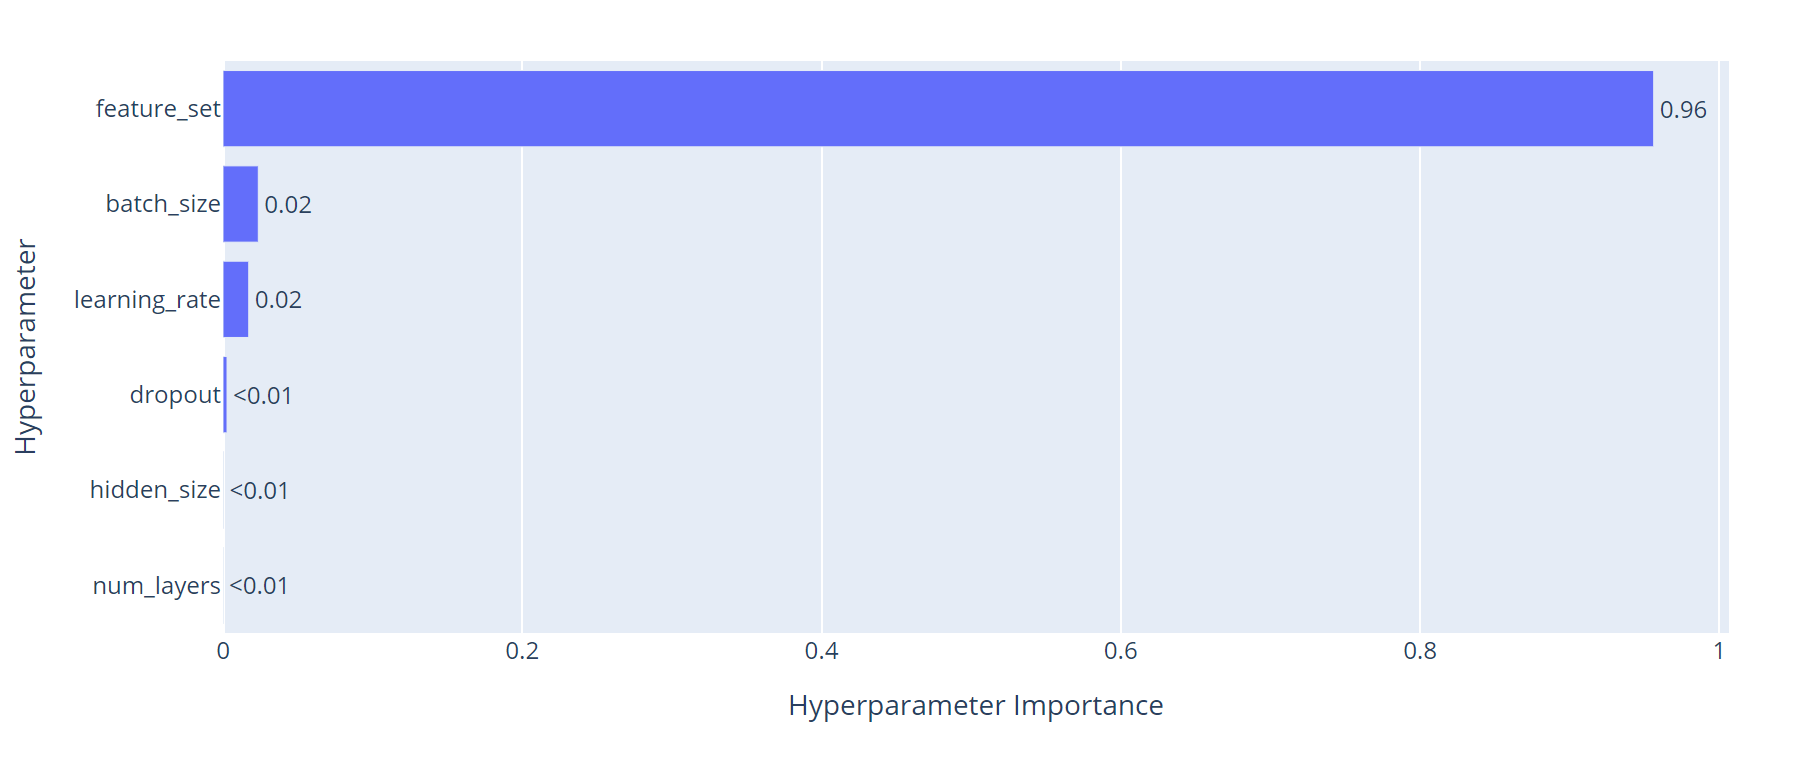
\includegraphics[width=0.95\linewidth]{figures/lstmhp.png}
    \caption[Hyperparameter Importances for the LSTM]{Quantitative hyperparameter importances for the \acf{LSTM}, calculated by Optuna using the \acf{fANOVA} framework. fANOVA isolates the marginal contribution of each parameter to the overall variance of the objective function, and thus provides quantitative metrics. The \texttt{feature\_set} dominates convergence success of the model by a significantly large margin. This high score must be interpreted with caution, as it is amplified by the evaluation bias detailed in Section \ref{lim:prior}. Conversely, \texttt{hidden\_size} registers an extremely low importance score; this matches with the observations from the parallel coordinate plot (Figure \ref{fig:paralelcord}), which demonstrated that exploring a wide range of hidden sizes had little to no impact on the final performance. Notably, \texttt{num\_layers} yields an importance of zero strictly because it was held constant and not defined as an active variable in this tuning space.}
    \label{fig:lstmhpimportances}
\end{figure}






\begin{comment}
\todo {weg mit den zweien die haben keinen mehrwert außer schau mal, eine statistik. außerdem istmissisipi noch drin}
\begin{figure}[ht]
\centering
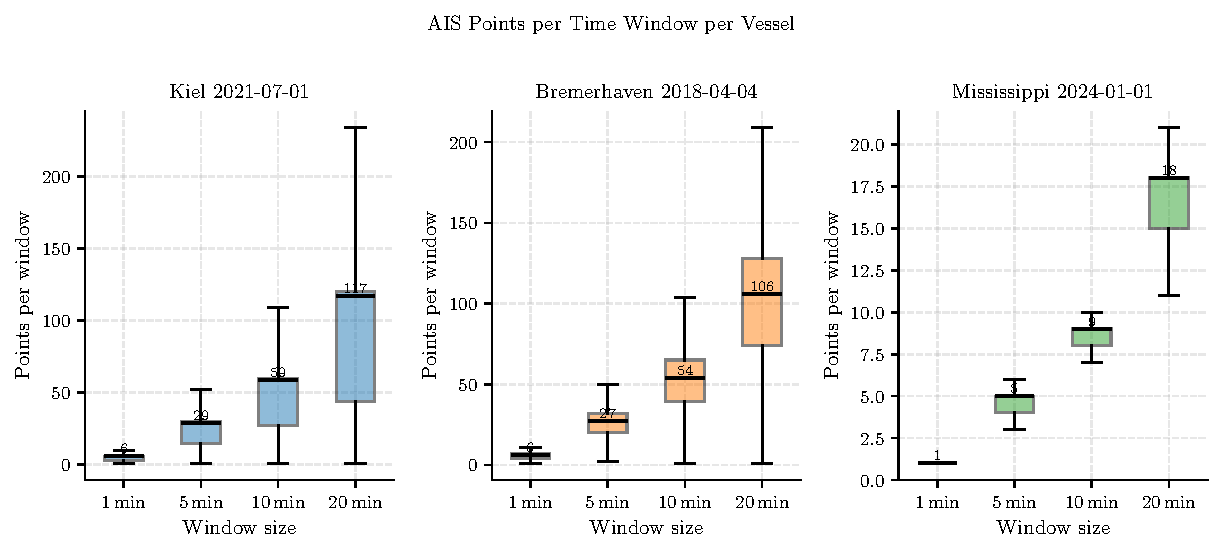
\includegraphics[width=1\textwidth]{figures/points_per_window.pdf}
\caption{Boxplot of AIS points per time window per vessel (sample day per dataset).}
\label{fig:points-per-window}
\end{figure}


\begin{figure}[ht]
\centering
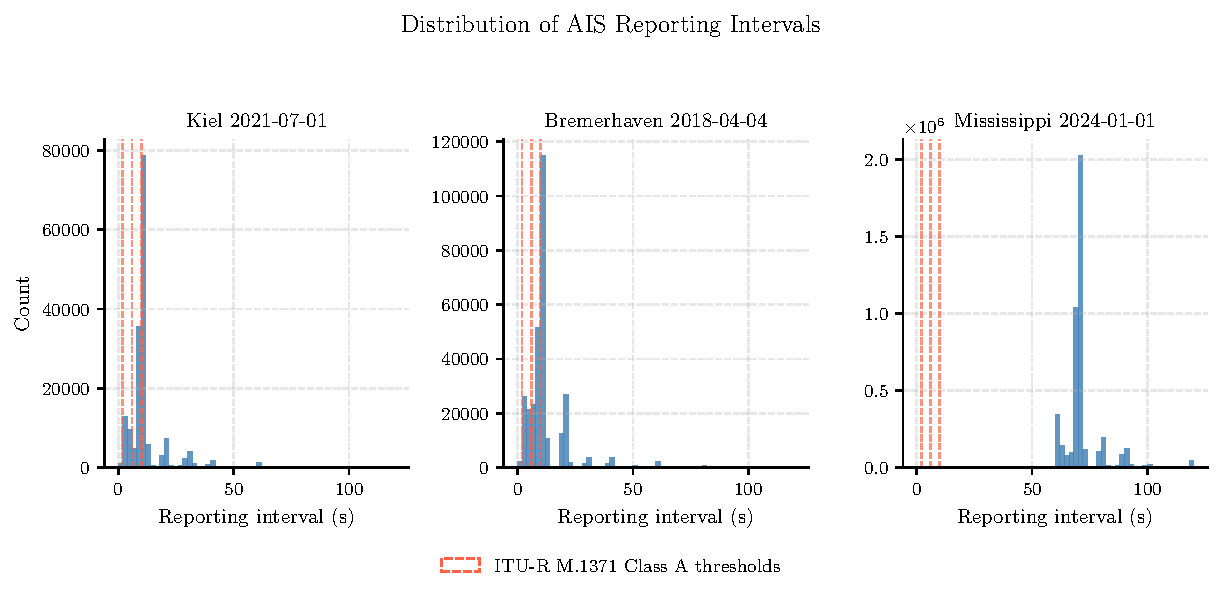
\includegraphics[width=1\textwidth]{figures/interval_hist.pdf}
\caption{Boxplot of inter-message intervals by velocity class.}
\label{fig:interval-hist}
\end{figure}
\end{comment}

%%%%%%sample trajectori4es

\FloatBarrier

% Optional: keep subfigure spacing tight
\captionsetup[subfigure]{justification=centering}

% =========================
% Domain 1 Channel
% =========================
\begin{figure}[p]
    \centering

    \begin{subfigure}[t]{0.6\textwidth}
        \centering
        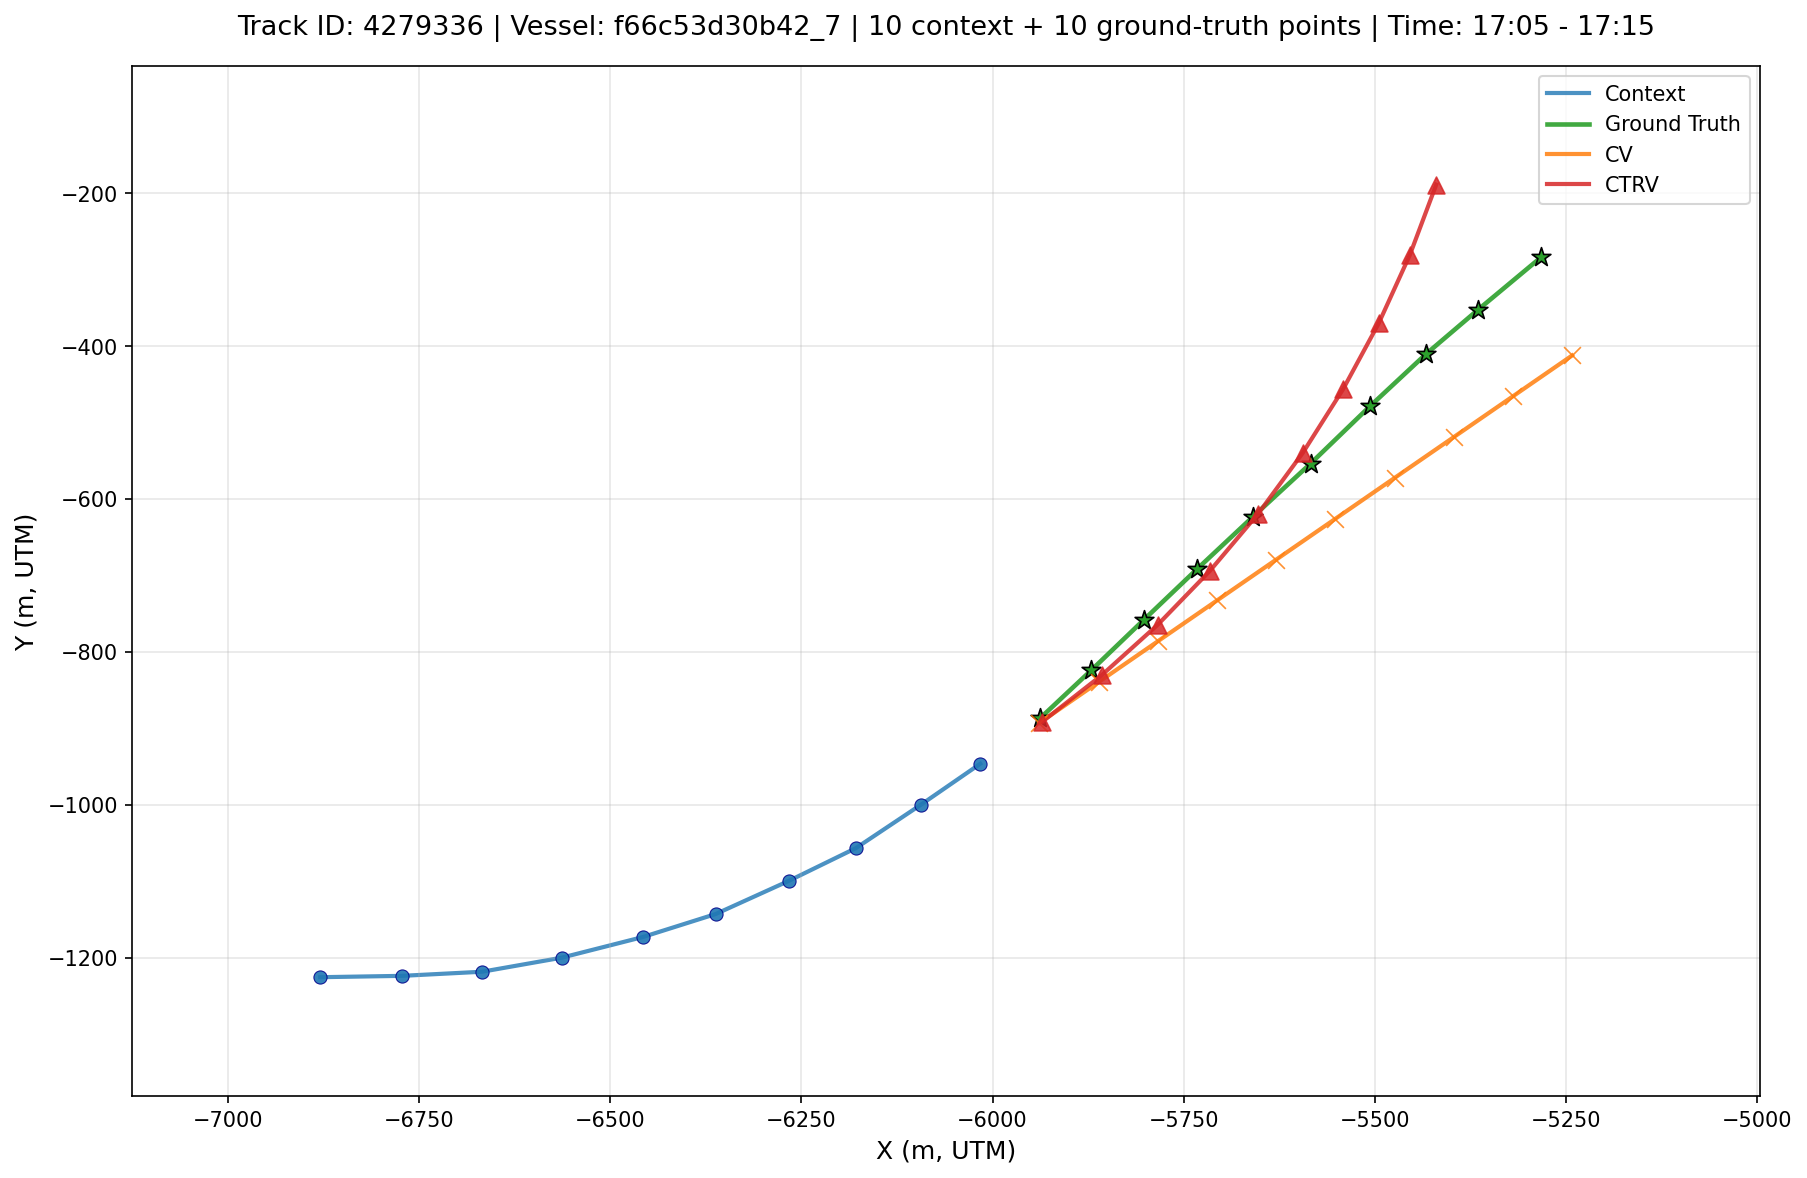
\includegraphics[width=\linewidth, trim=0 0 0cm 1.6cm,clip]{figures/domain11.png}
    \end{subfigure}

    \vspace{0.5em}

    \begin{subfigure}[t]{0.6\textwidth}
        \centering
        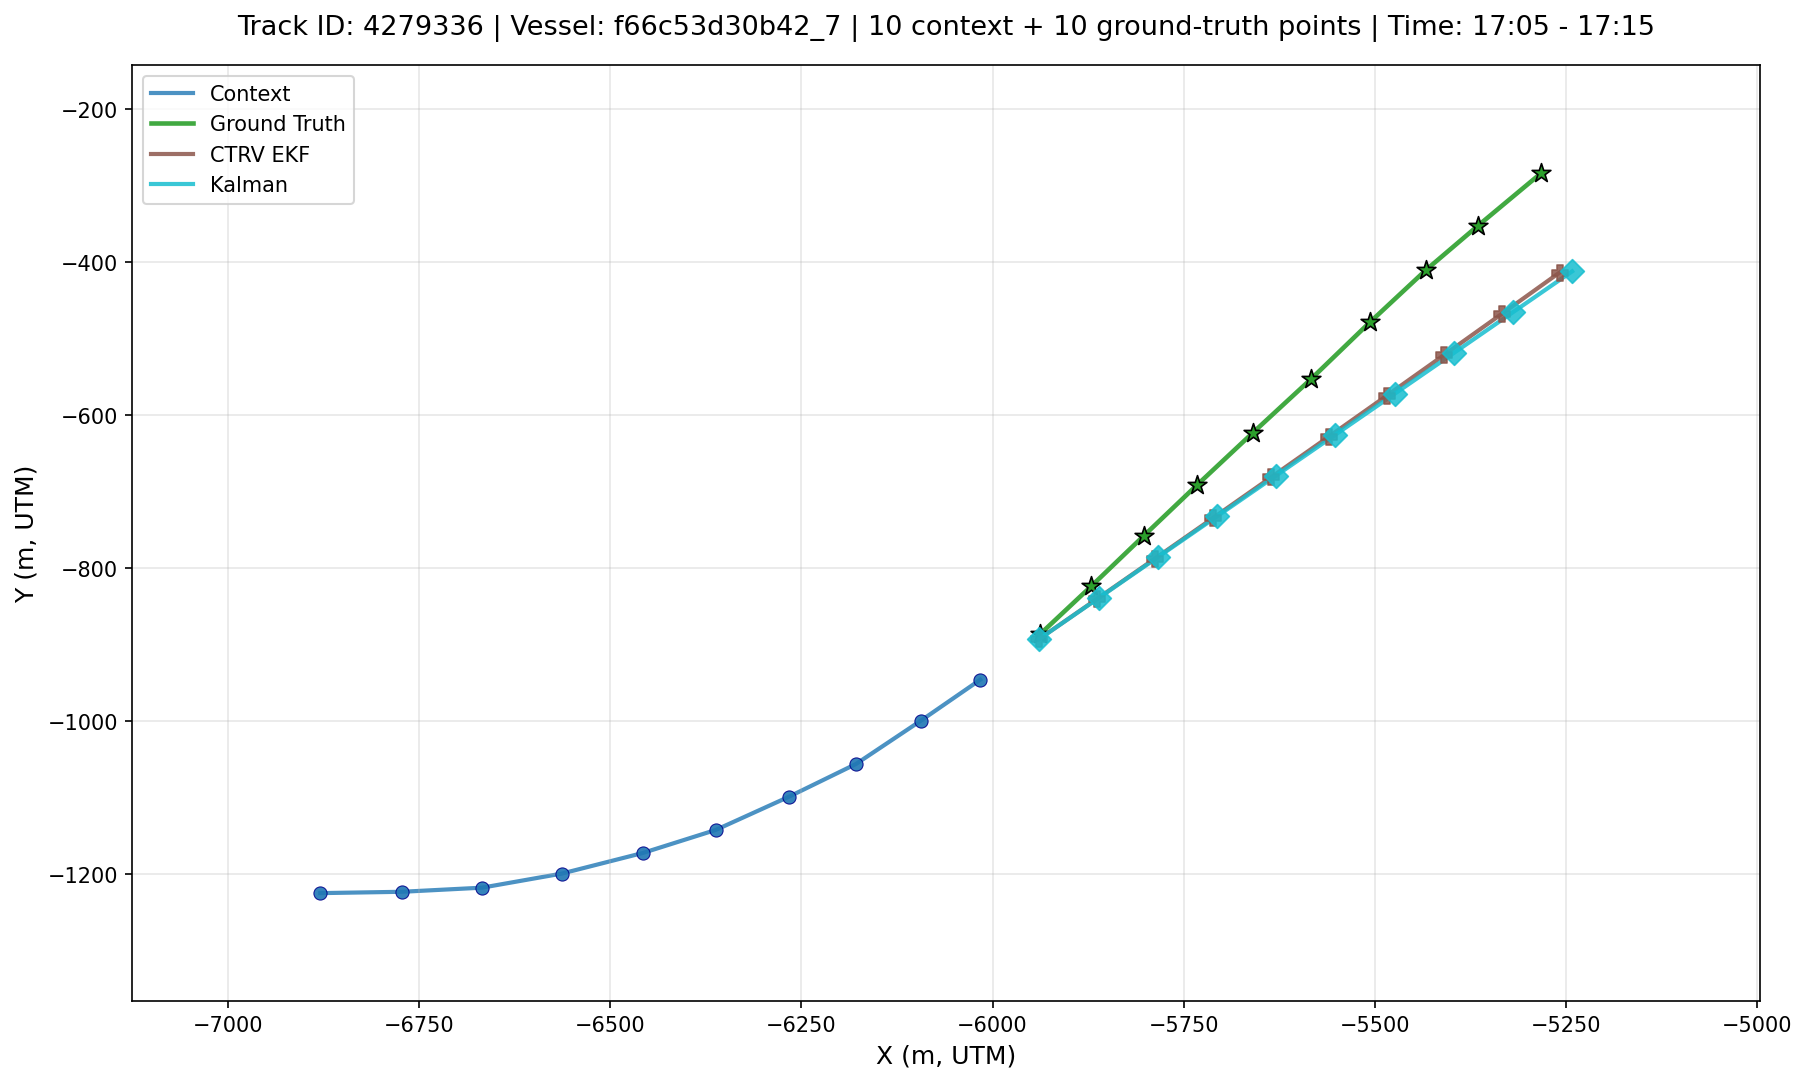
\includegraphics[width=\linewidth, trim=0 0 0cm 1.6cm,clip]{figures/domain12.png}
    \end{subfigure}

    \vspace{0.5em}

    \begin{subfigure}[t]{0.6\textwidth}
        \centering
        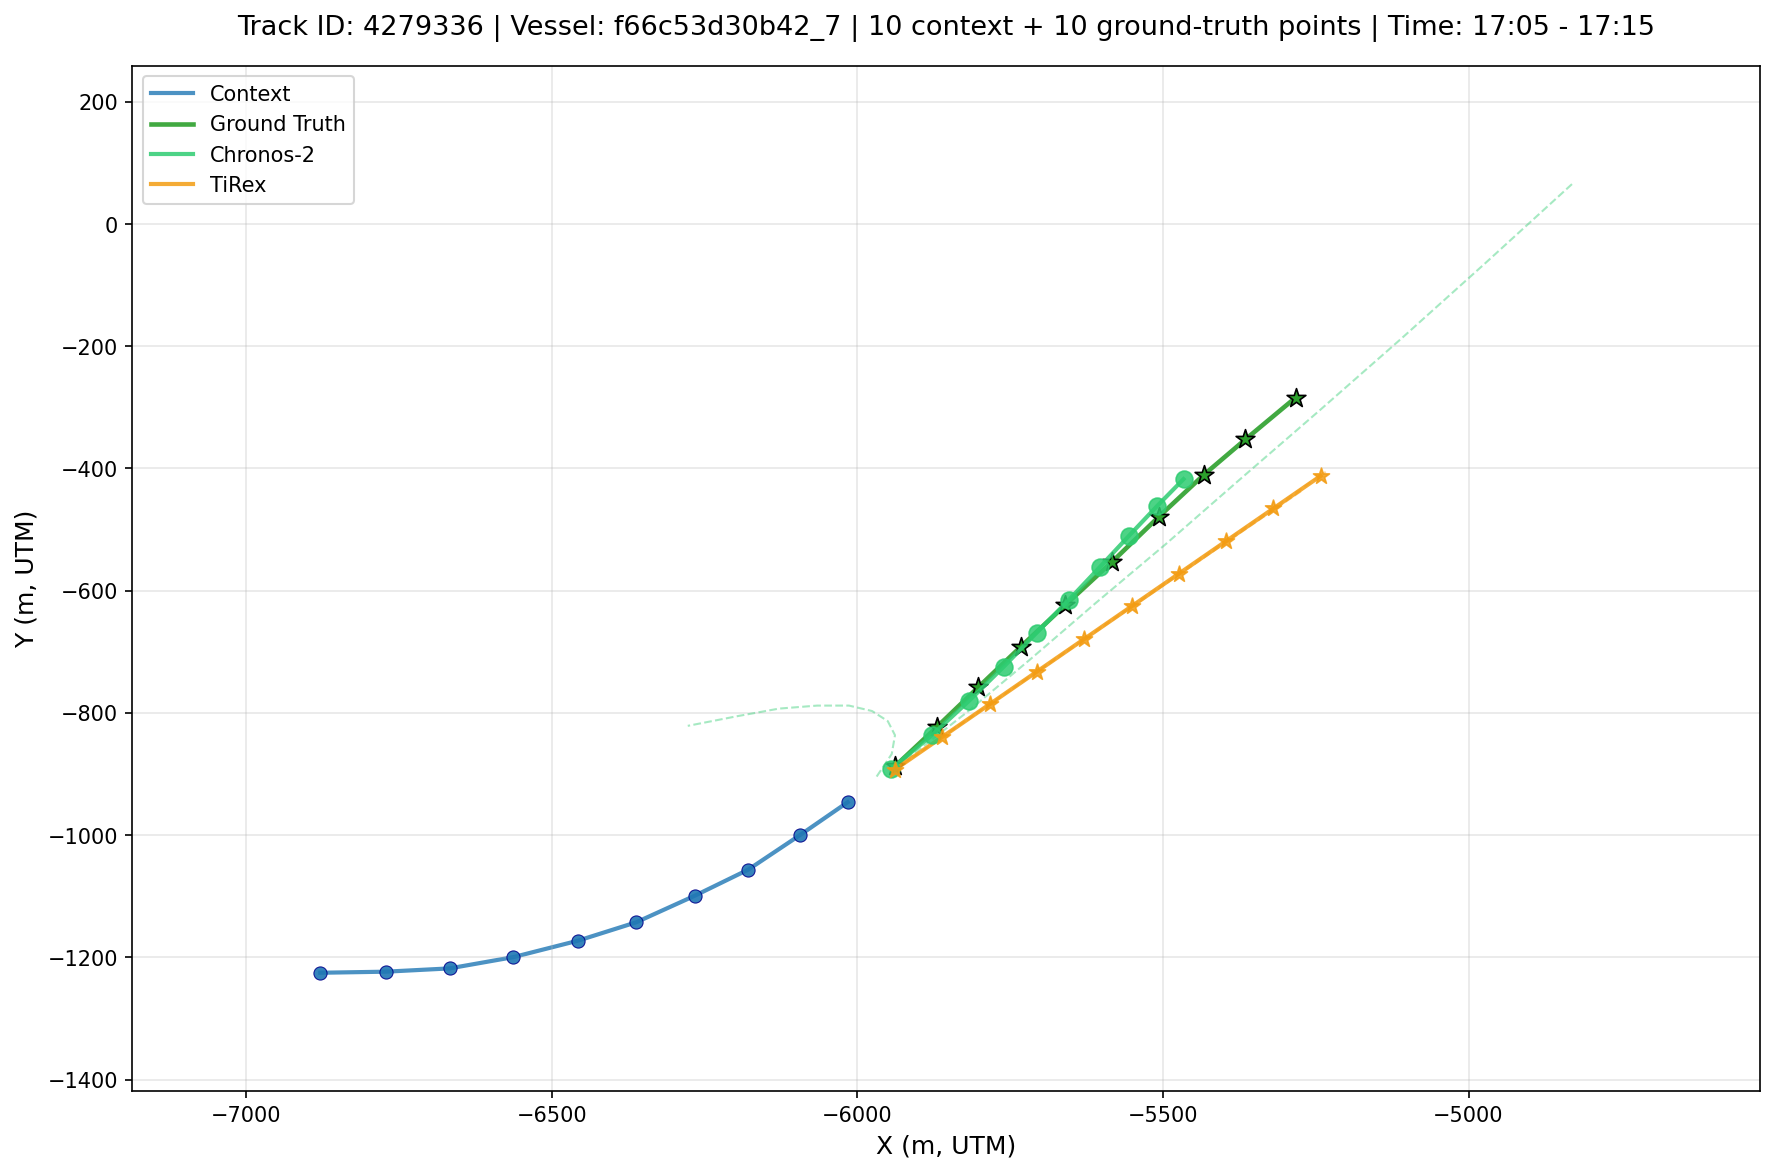
\includegraphics[width=\linewidth, trim=0 0 0cm 1.6cm,clip]{figures/domain13.png}
    \end{subfigure}

    \vspace{0.5em}

    \begin{subfigure}[t]{0.6\textwidth}
        \centering
        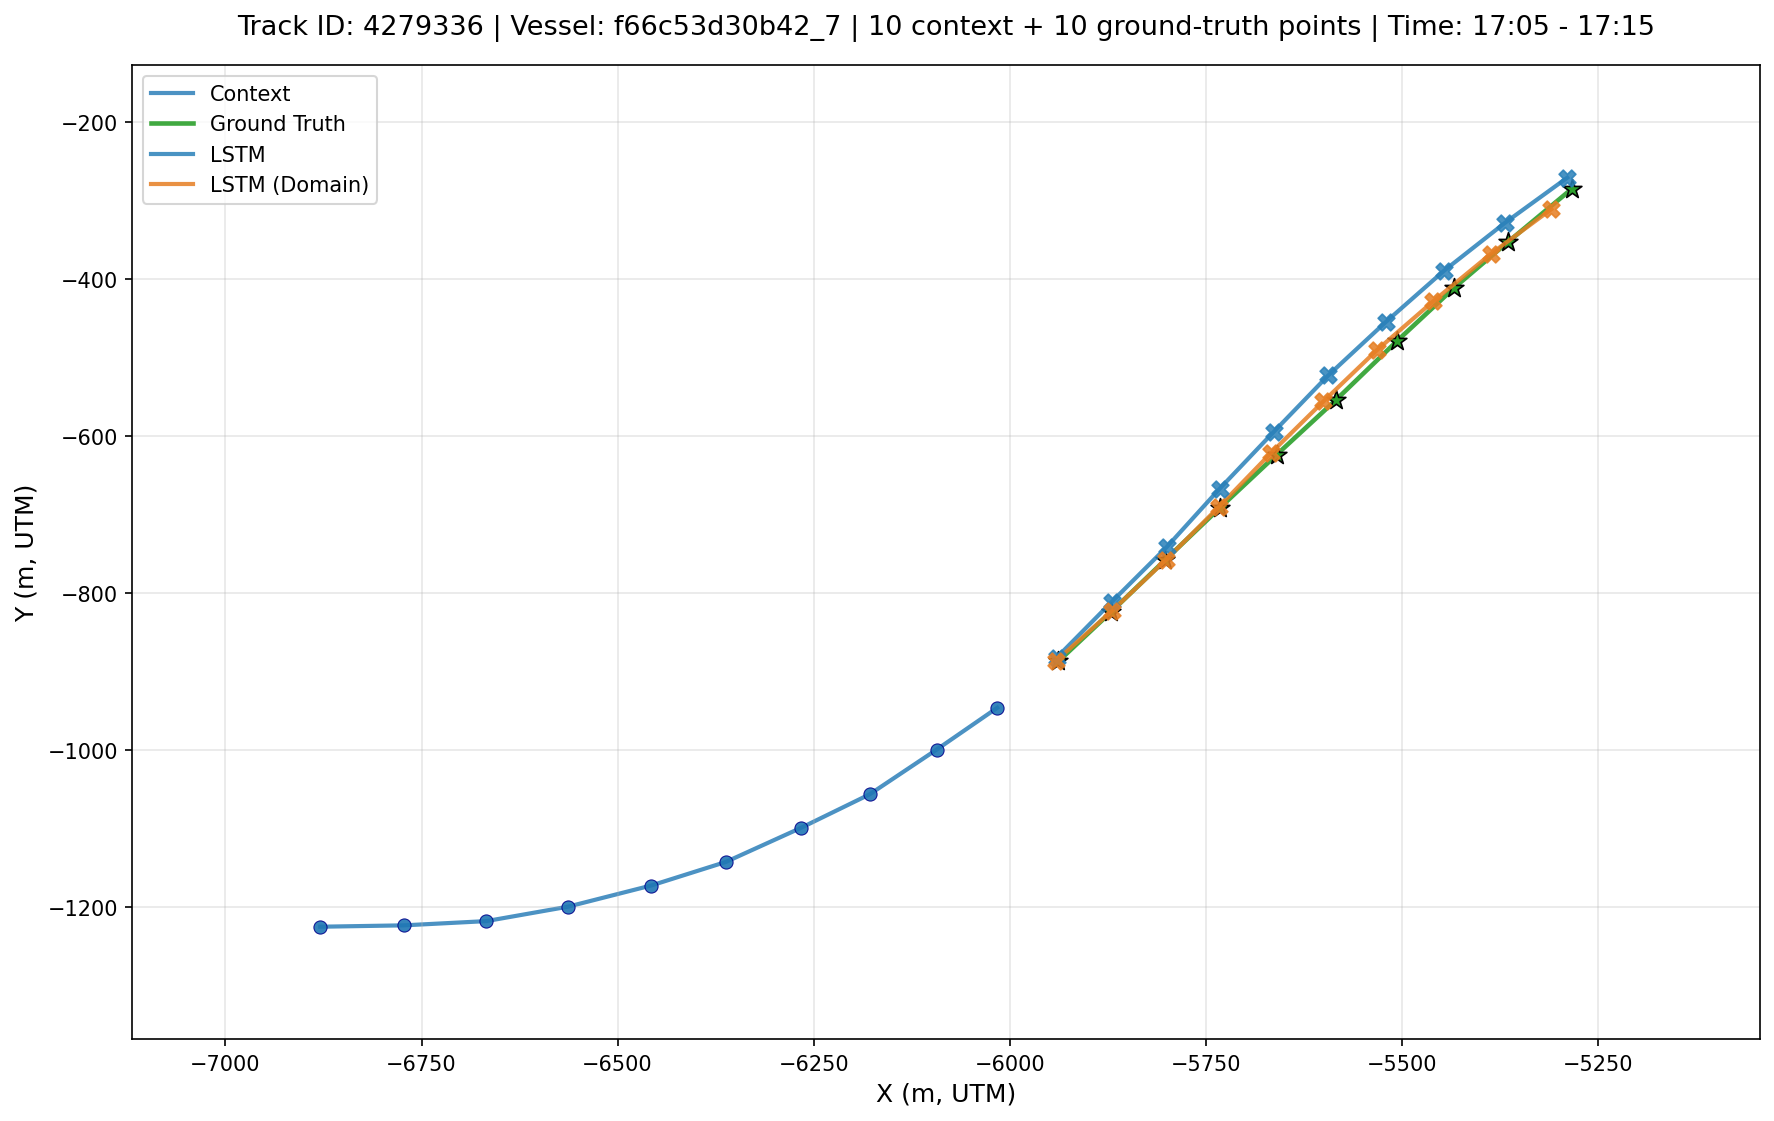
\includegraphics[width=\linewidth, trim=0 0 0cm 1.6cm,clip]{figures/domain14.png}
    \end{subfigure}


    \caption[Forecasting examples for Channel (Kiel)]{Forecasting examples for the Channel domain (Kiel). These plots provide a qualitative visual comparison of the predicted paths generated by the evaluated models. The observed context window is displayed in blue, while the actual ground truth trajectory that follows is marked with green stars. The various model predictions are shown in the remaining colours. For Chronos 2, the 80\% certainty band is displayed using thin green dots. Both axes represent relative \ac{UTM} coordinates measured in meters.}
    \label{fig:domain1}
\end{figure}

\FloatBarrier
\clearpage

% =========================
% Domain 2
% =========================
\begin{figure}[p]
    \centering

    \begin{subfigure}[t]{0.49\textwidth}
        \centering
        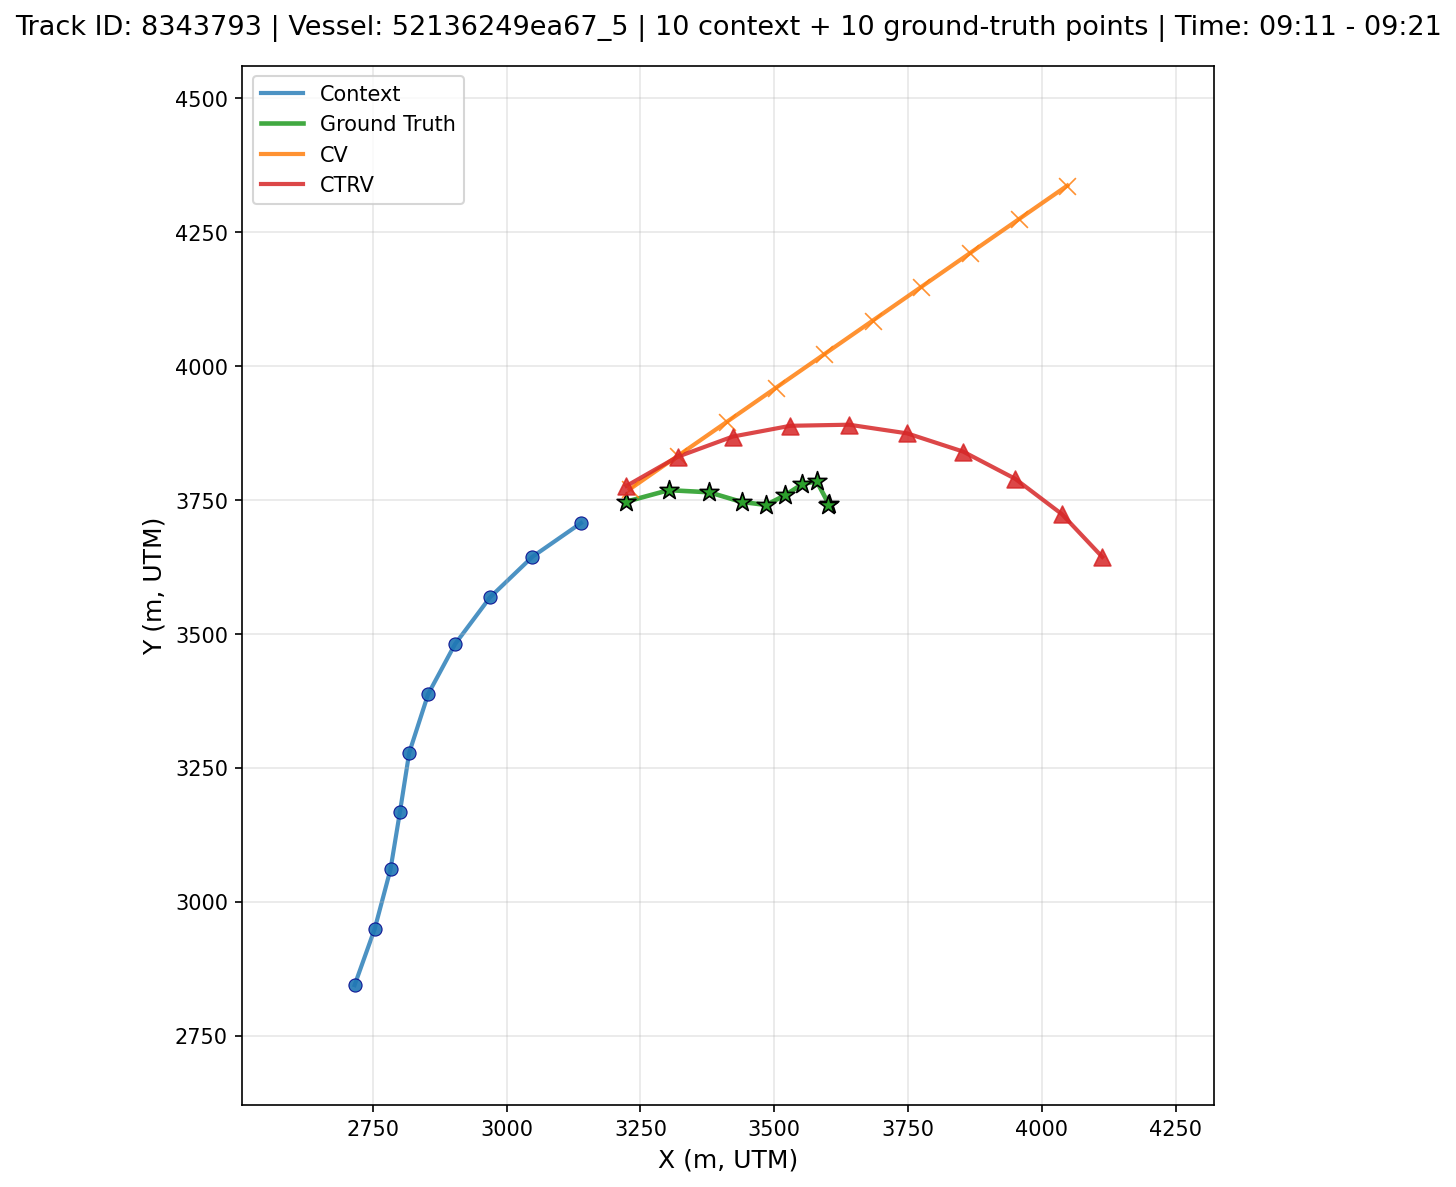
\includegraphics[width=\linewidth, trim=0 0 0cm 1.6cm,clip]{figures/domain21.png}
    \end{subfigure}
    \hfill
    \begin{subfigure}[t]{0.49\textwidth}
        \centering
        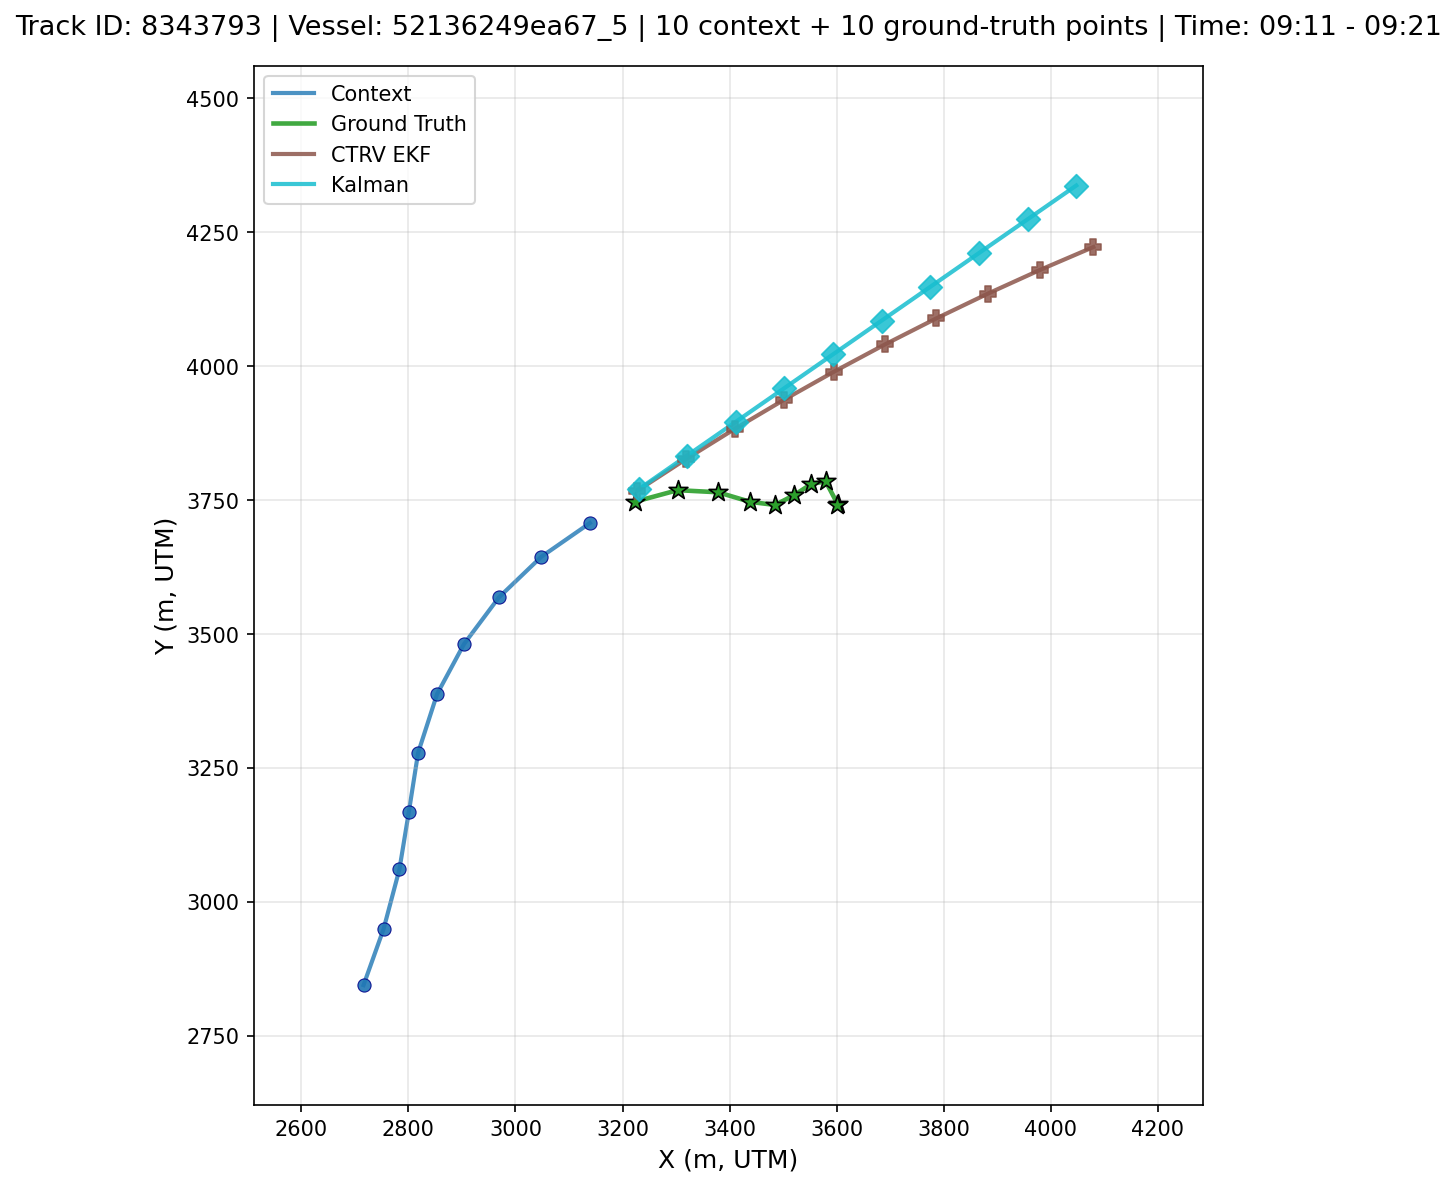
\includegraphics[width=\linewidth, trim=0 0 0cm 1.6cm,clip]{figures/domain22.png}
    \end{subfigure}

    \vspace{0.5em}

    \begin{subfigure}[t]{0.49\textwidth}
        \centering
        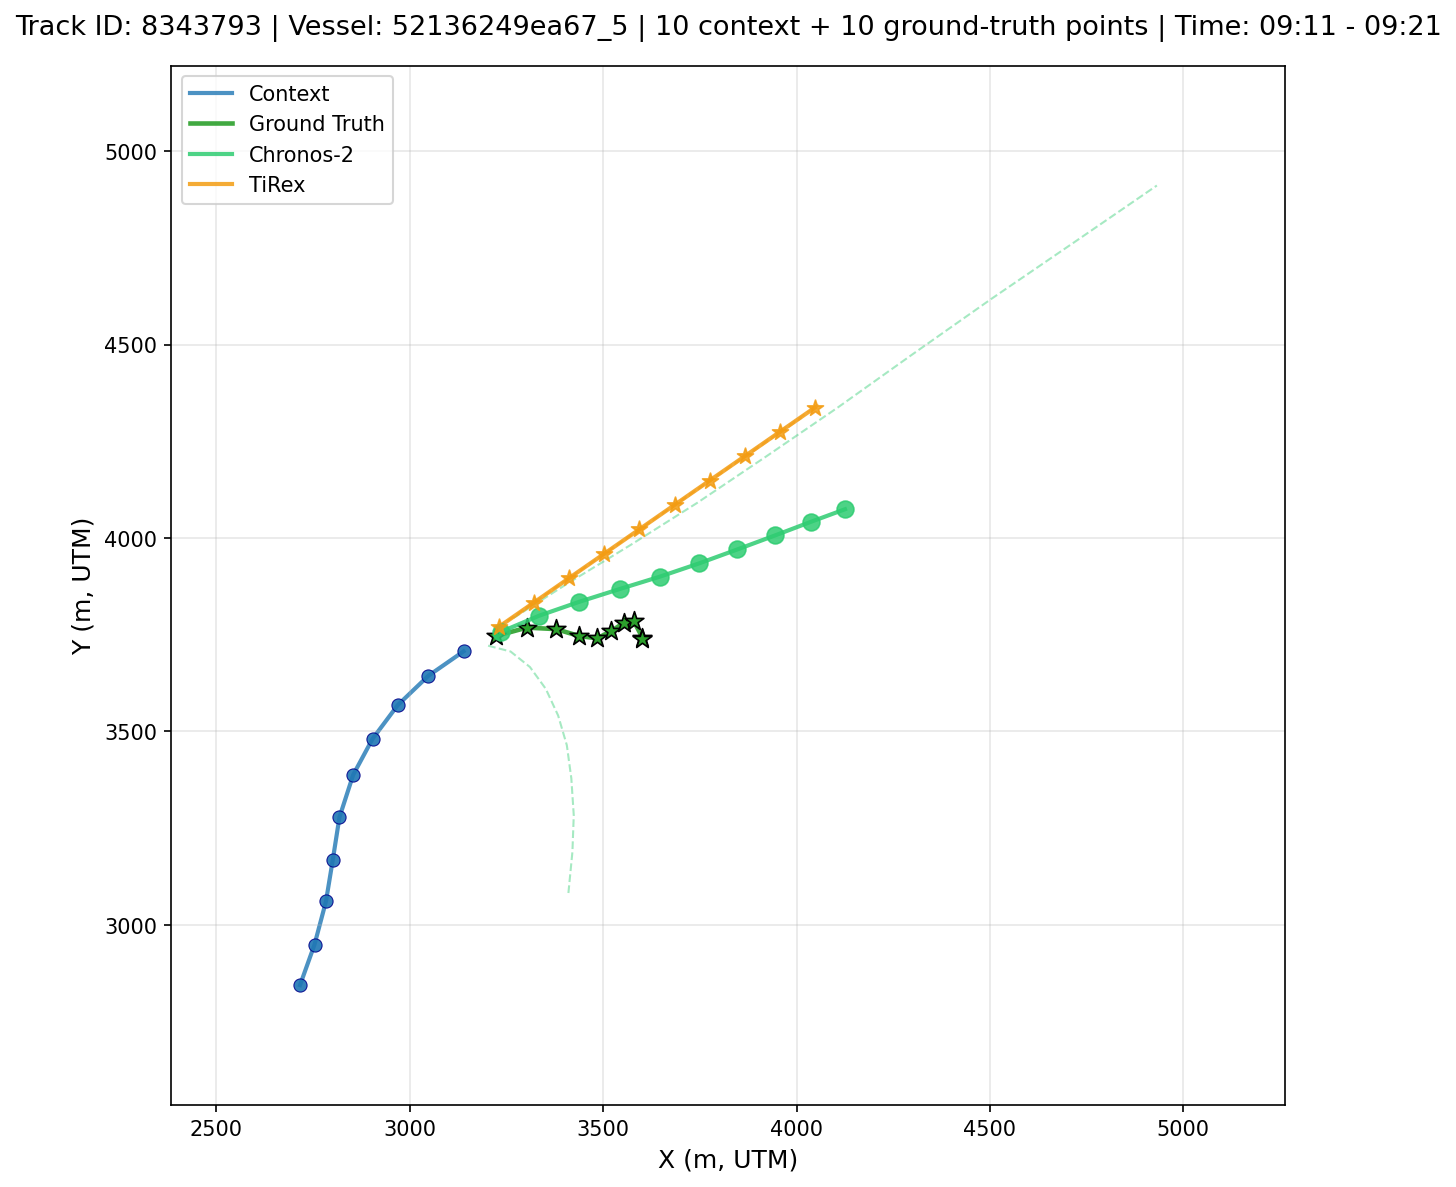
\includegraphics[width=\linewidth, trim=0 0 0cm 1.6cm,clip]{figures/domain23.png}
    \end{subfigure}
    \hfill
    \begin{subfigure}[t]{0.49\textwidth}
        \centering
        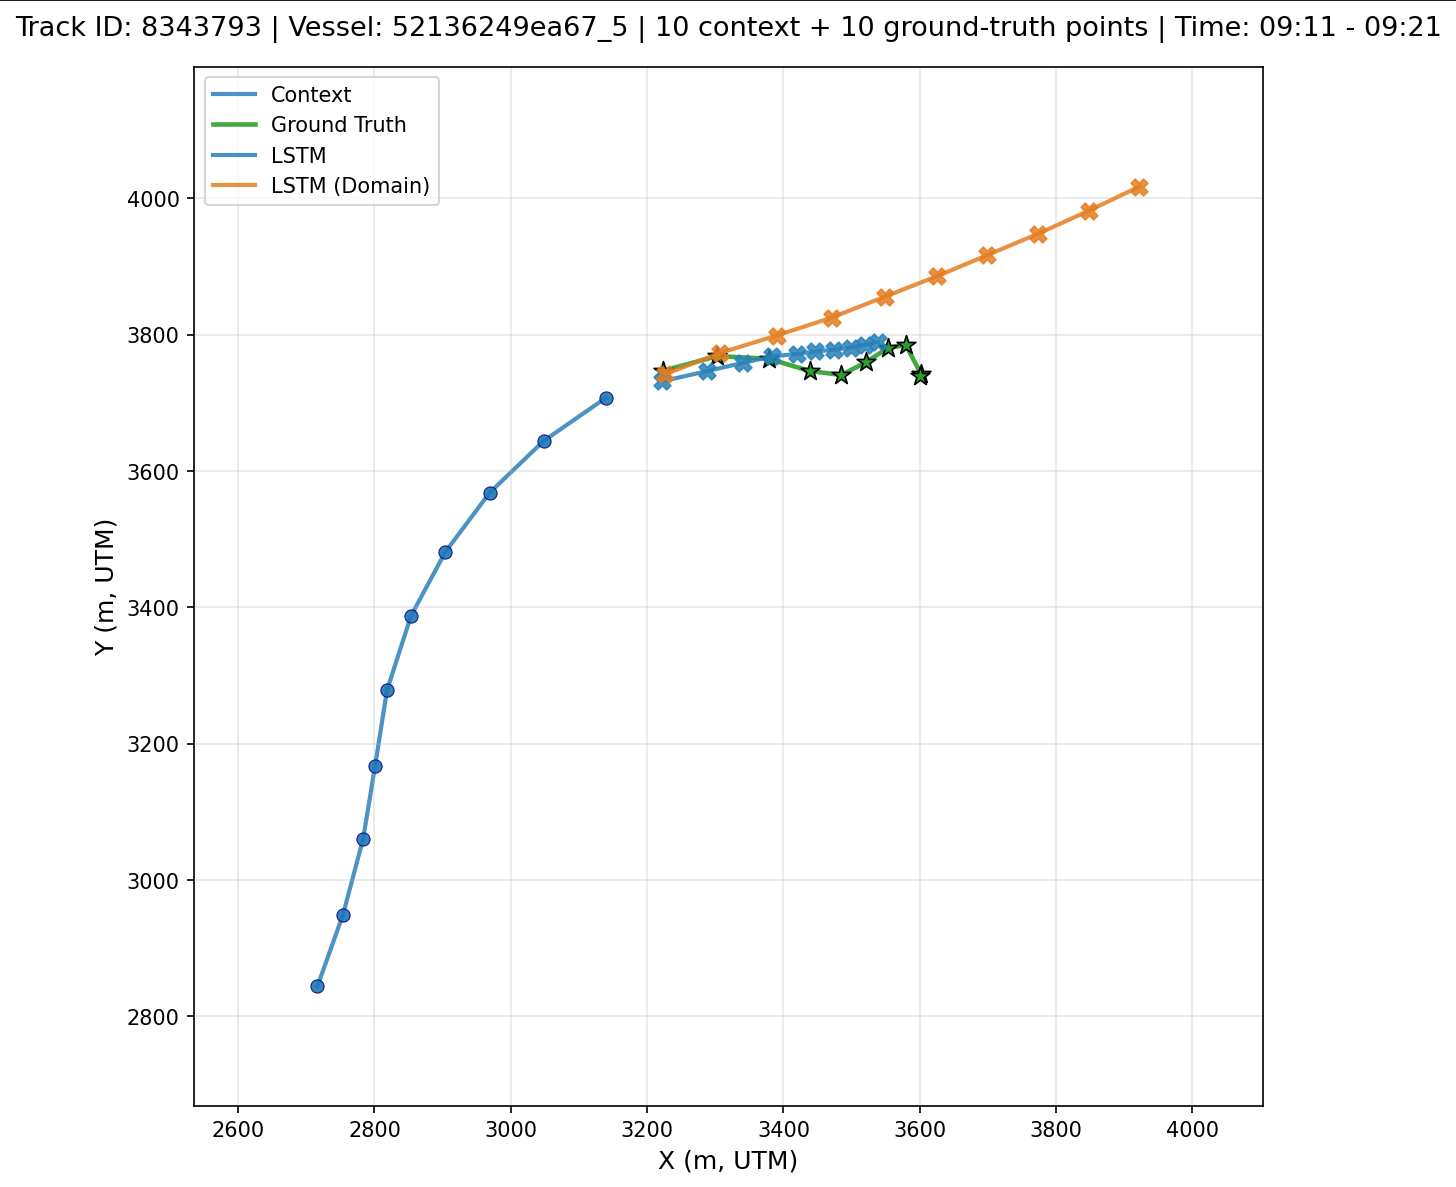
\includegraphics[width=\linewidth, trim=0 0 0cm 1.6cm,clip]{figures/domain24.png}
    \end{subfigure}

    \caption[Forecasting examples for Harbour (Kiel)]{Forecasting examples for the Harbour domain (Kiel). These plots provide a qualitative visual comparison of the predicted paths generated by the evaluated models. The observed context window is displayed in blue, while the actual ground truth trajectory that follows is marked with green stars. The various model predictions are shown in the remaining colours. For Chronos 2, the 80\% certainty band is displayed using thin green dots. Both axes represent relative \ac{UTM} coordinates measured in meters.}    \label{fig:domain2}
\end{figure}

\FloatBarrier
\clearpage

% =========================
% Domain 3
% =========================
\begin{figure}[p]
    \centering

    \begin{subfigure}[t]{0.95\textwidth}
        \centering
        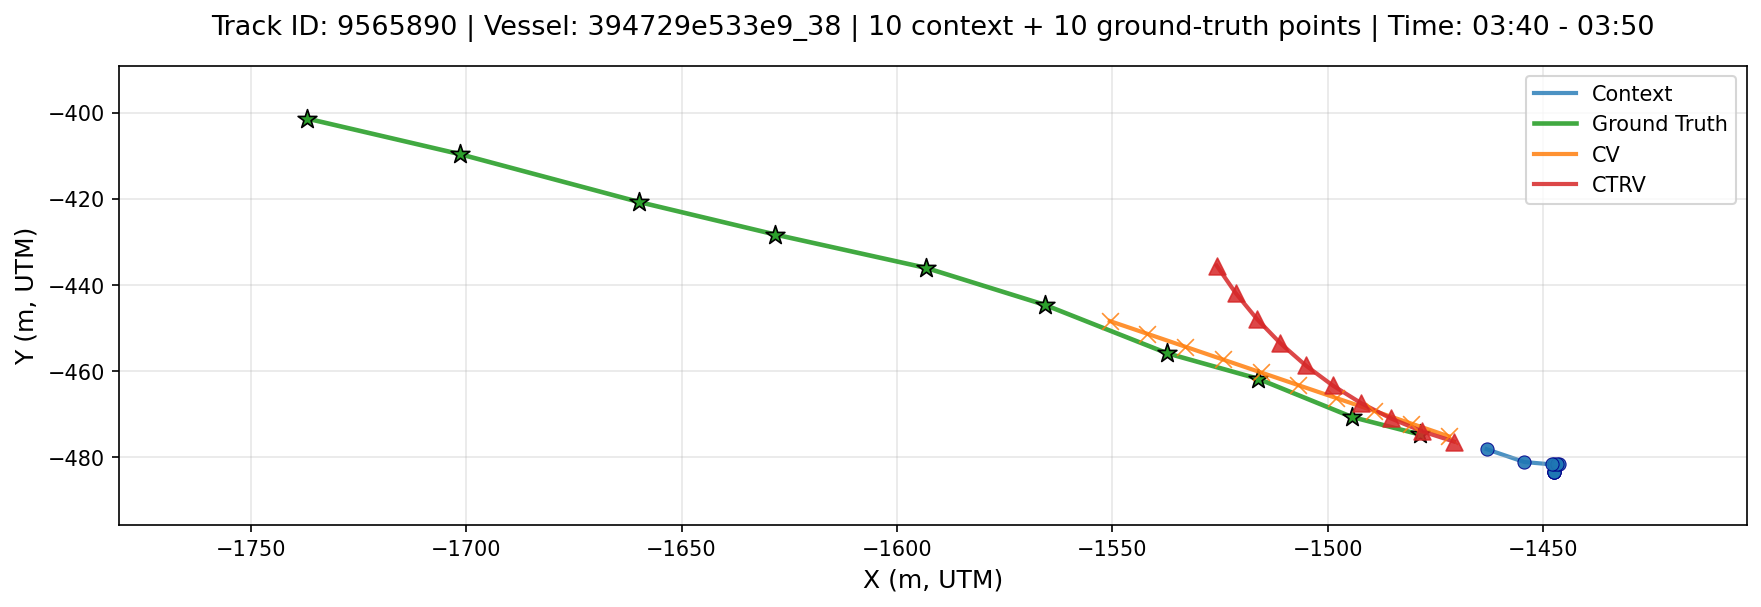
\includegraphics[width=\linewidth, trim=0 0 0cm 1.5cm,clip]{figures/domain31.png}
    \end{subfigure}

    \vspace{0.5em}

    \begin{subfigure}[t]{0.95\textwidth}
        \centering
        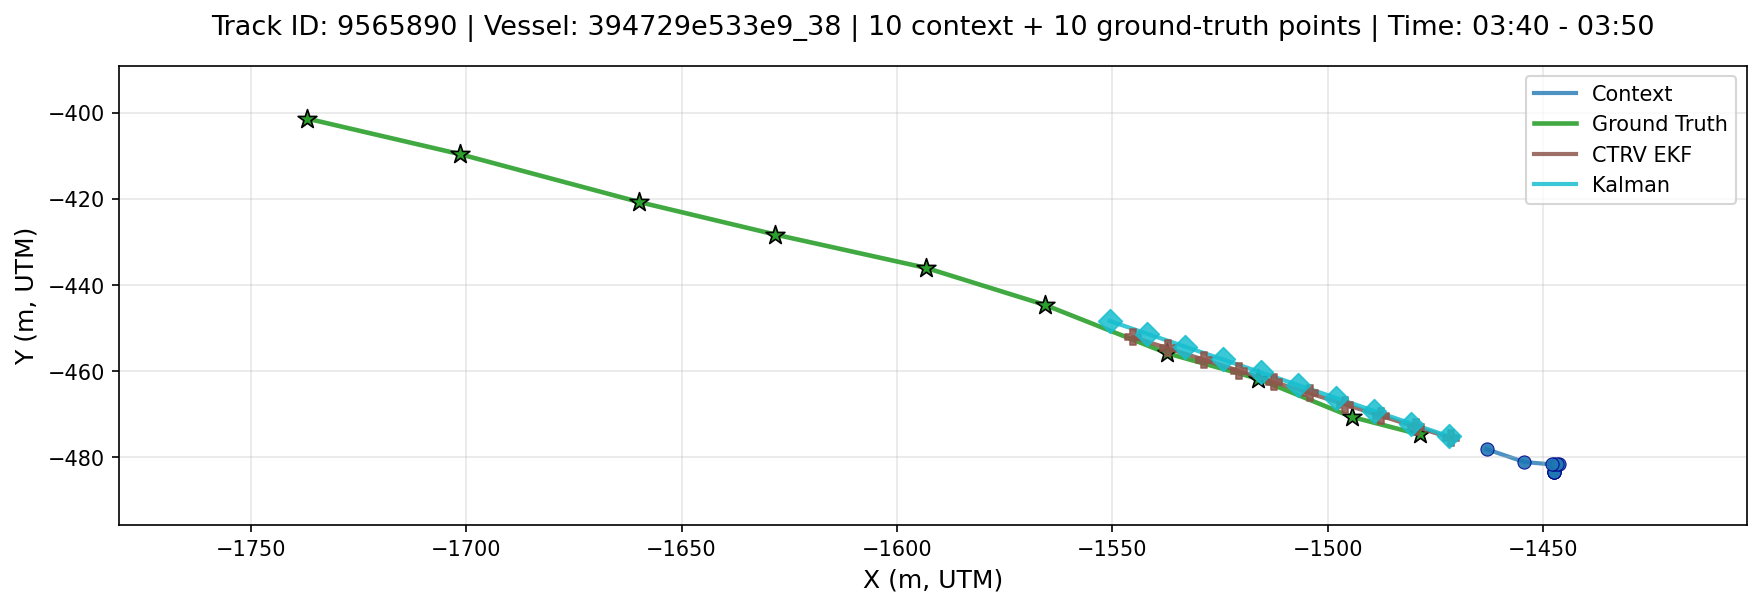
\includegraphics[width=\linewidth, trim=0 0 0cm 1.5cm,clip]{figures/domain32.png}
    \end{subfigure}

    \vspace{0.5em}

    \begin{subfigure}[t]{0.95\textwidth}
        \centering
        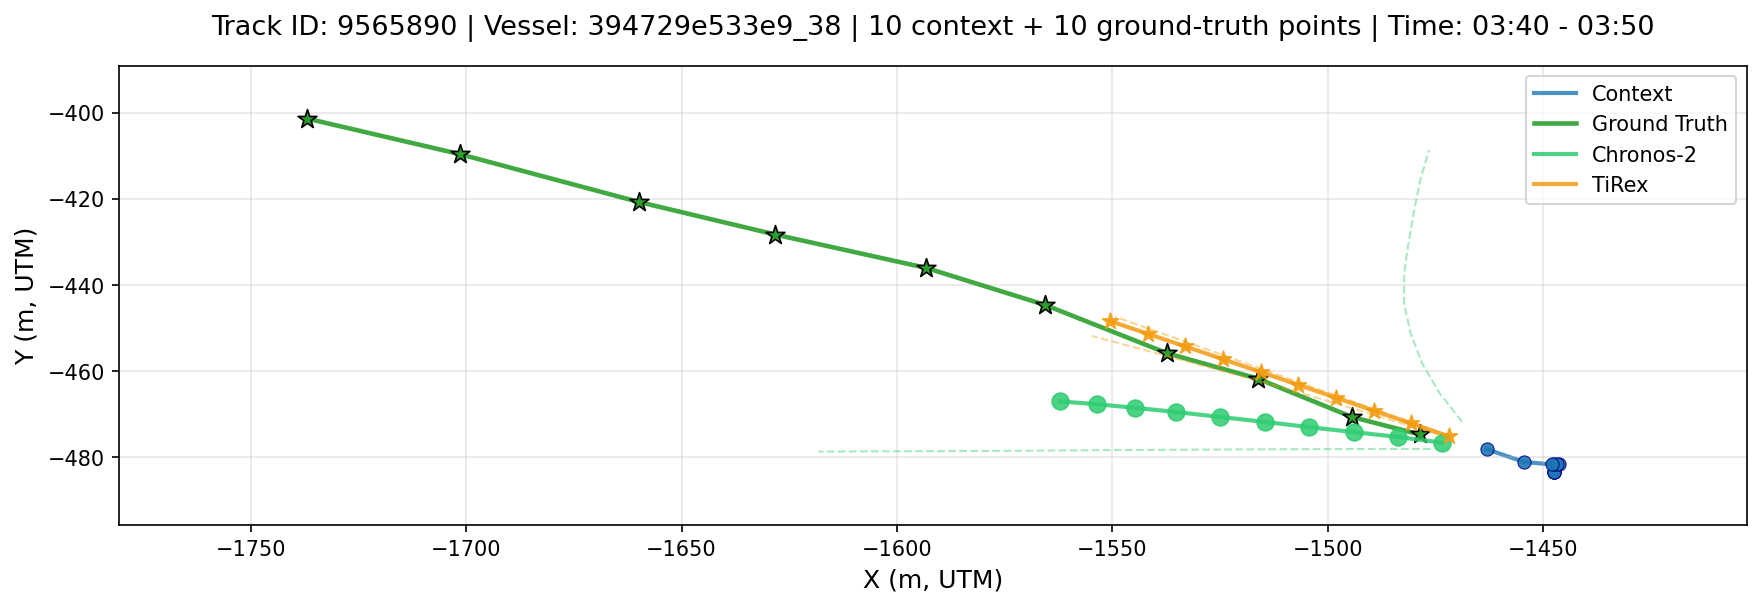
\includegraphics[width=\linewidth, trim=0 0 0cm 1.5cm,clip]{figures/domain33.png}
    \end{subfigure}

    \vspace{0.5em}

    \begin{subfigure}[t]{0.95\textwidth}
        \centering
        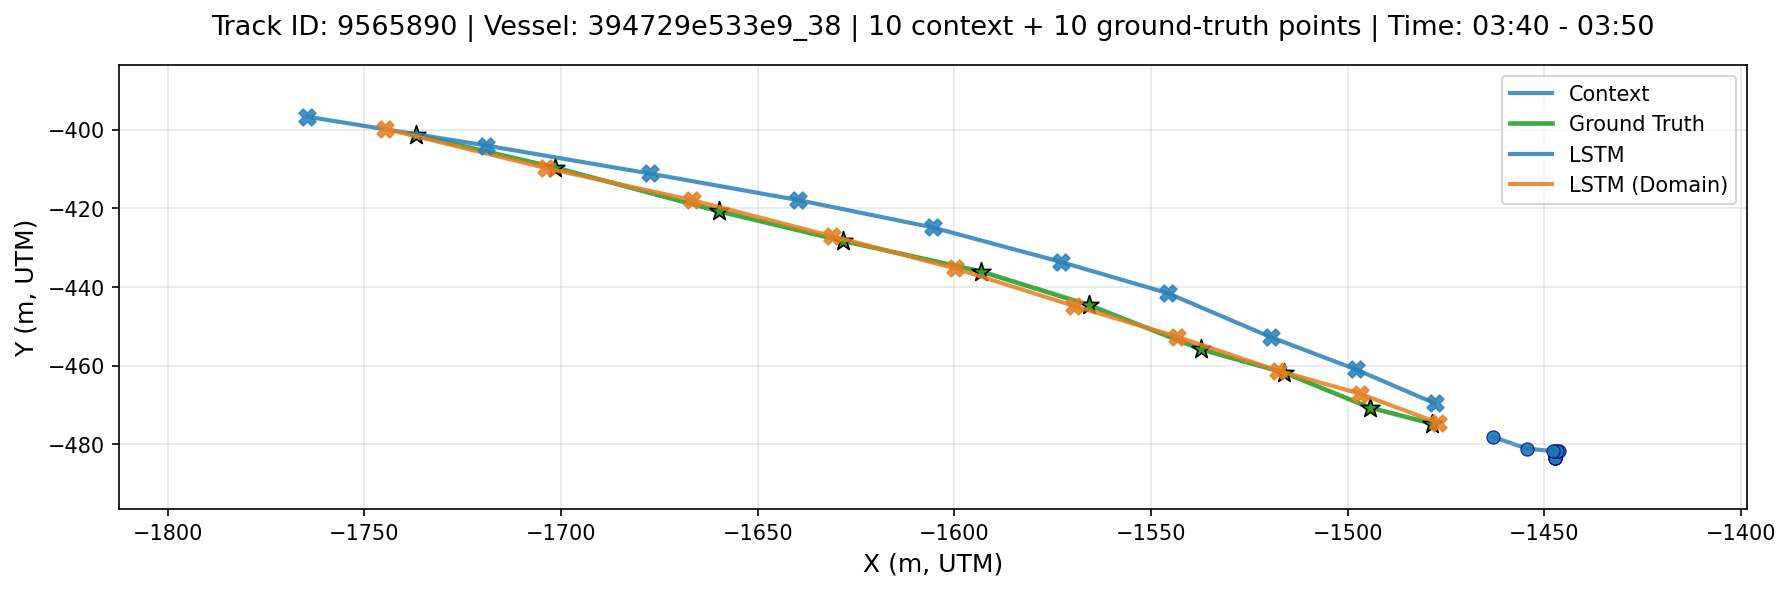
\includegraphics[width=\linewidth, trim=0 0 0cm 1.5cm,clip]{figures/domain34.png}
    \end{subfigure}

    \caption[Forecasting examples for Lock (Kiel)]{Forecasting examples for the Lock domain (Kiel). These plots provide a qualitative visual comparison of the predicted paths generated by the evaluated models. The observed context window is displayed in blue, while the actual ground truth trajectory that follows is marked with green stars. The various model predictions are shown in the remaining colours. For Chronos 2, the 80\% certainty band is displayed using thin green dots. Both axes represent relative \ac{UTM} coordinates measured in meters.}    \label{fig:domain3}
\end{figure}

\FloatBarrier
\clearpage

% =========================
% Domain 4
% =========================
\begin{figure}[p]
    \centering

    \begin{subfigure}[t]{0.95\textwidth}
        \centering
        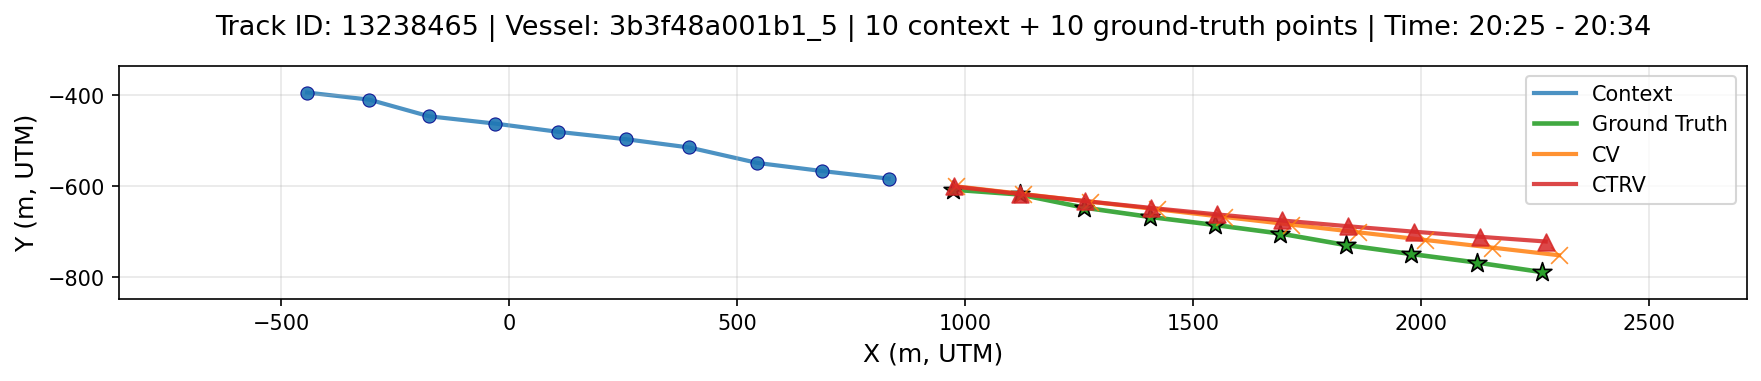
\includegraphics[width=\linewidth, trim=0 0 0cm 1.5cm,clip]{figures/domain41.png}
    \end{subfigure}

    \vspace{0.5em}

    \begin{subfigure}[t]{0.95\textwidth}
        \centering
        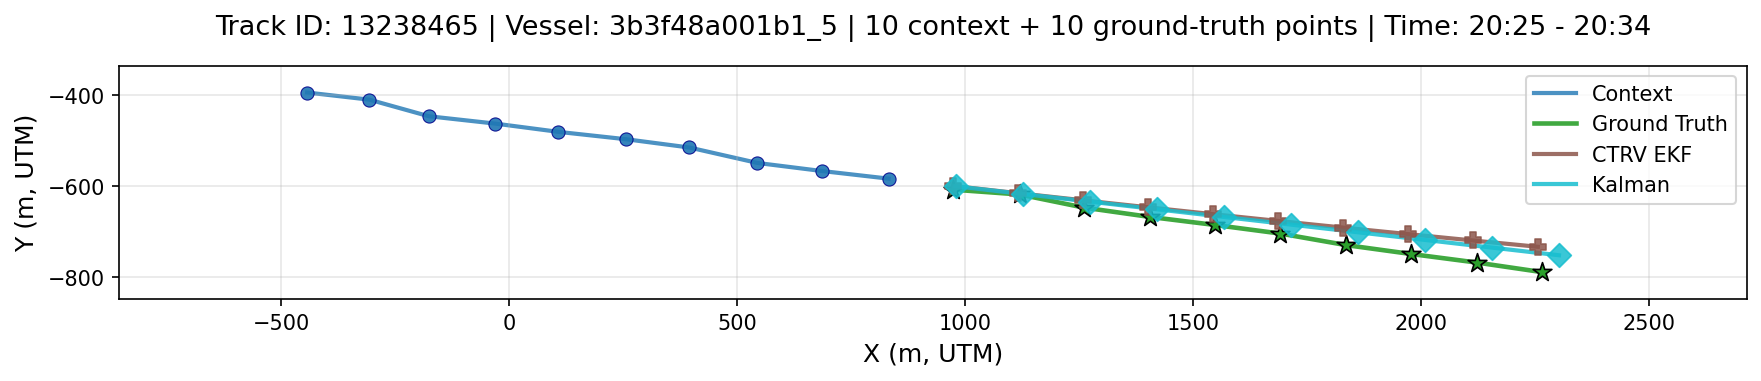
\includegraphics[width=\linewidth, trim=0 0 0cm 1.5cm,clip]{figures/domain42.png}
    \end{subfigure}

    \vspace{0.5em}

    \begin{subfigure}[t]{0.95\textwidth}
        \centering
        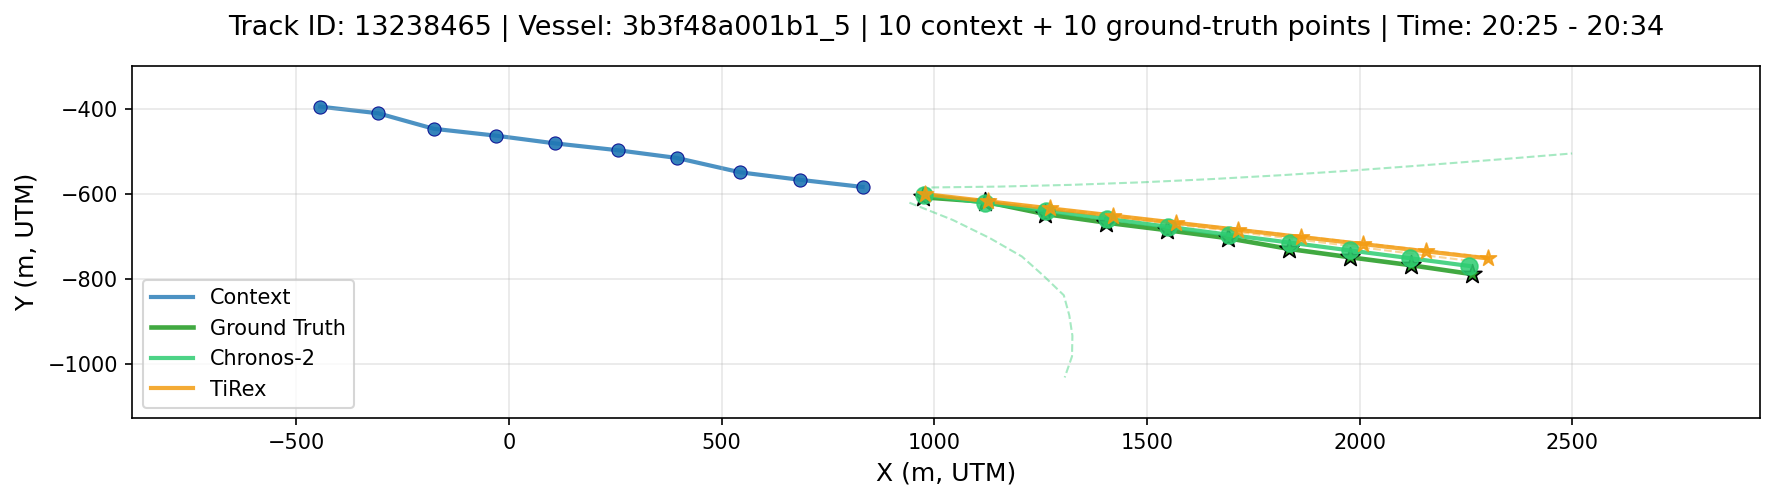
\includegraphics[width=\linewidth, trim=0 0 0cm 1.5cm,clip]{figures/domain43.png}
    \end{subfigure}

    \vspace{0.5em}

    \begin{subfigure}[t]{0.95\textwidth}
        \centering
        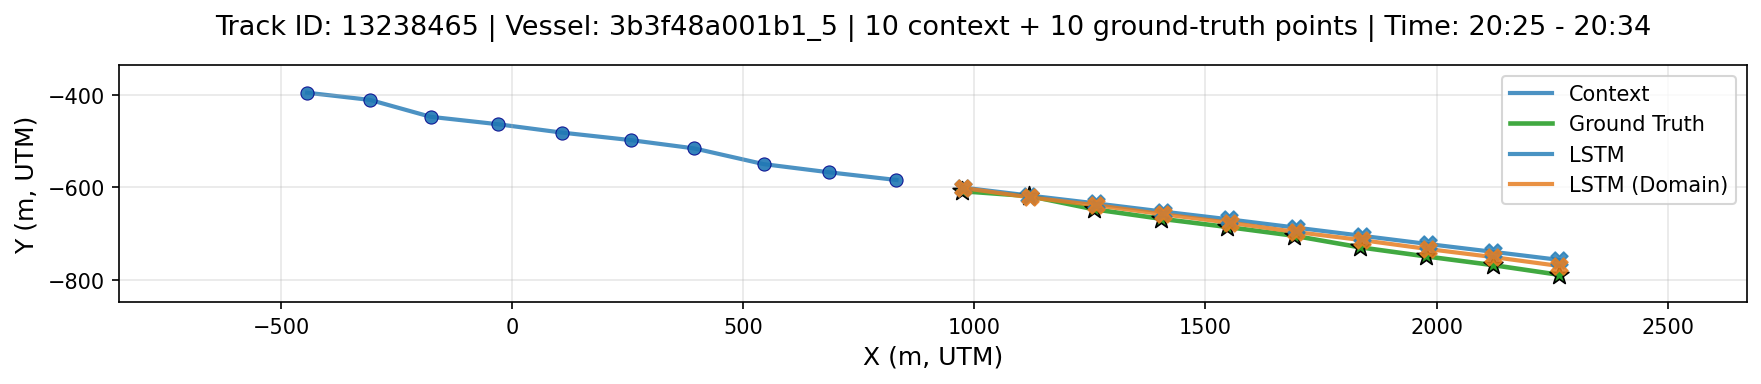
\includegraphics[width=\linewidth, trim=0 0 0cm 1.5cm,clip]{figures/domain44.png}
    \end{subfigure}

    \caption[Forecasting examples for River (Wedel)]{Forecasting examples for the River domain (Wedel). These plots provide a qualitative visual comparison of the predicted paths generated by the evaluated models. The observed context window is displayed in blue, while the actual ground truth trajectory that follows is marked with green stars. The various model predictions are shown in the remaining colours. For Chronos 2, the 80\% certainty band is displayed using thin green dots. Both axes represent relative \ac{UTM} coordinates measured in meters.}    \label{fig:domain4}
\end{figure}








% Seite 1: CD Diagrams 1–2
\begin{figure}[p]
    \centering
    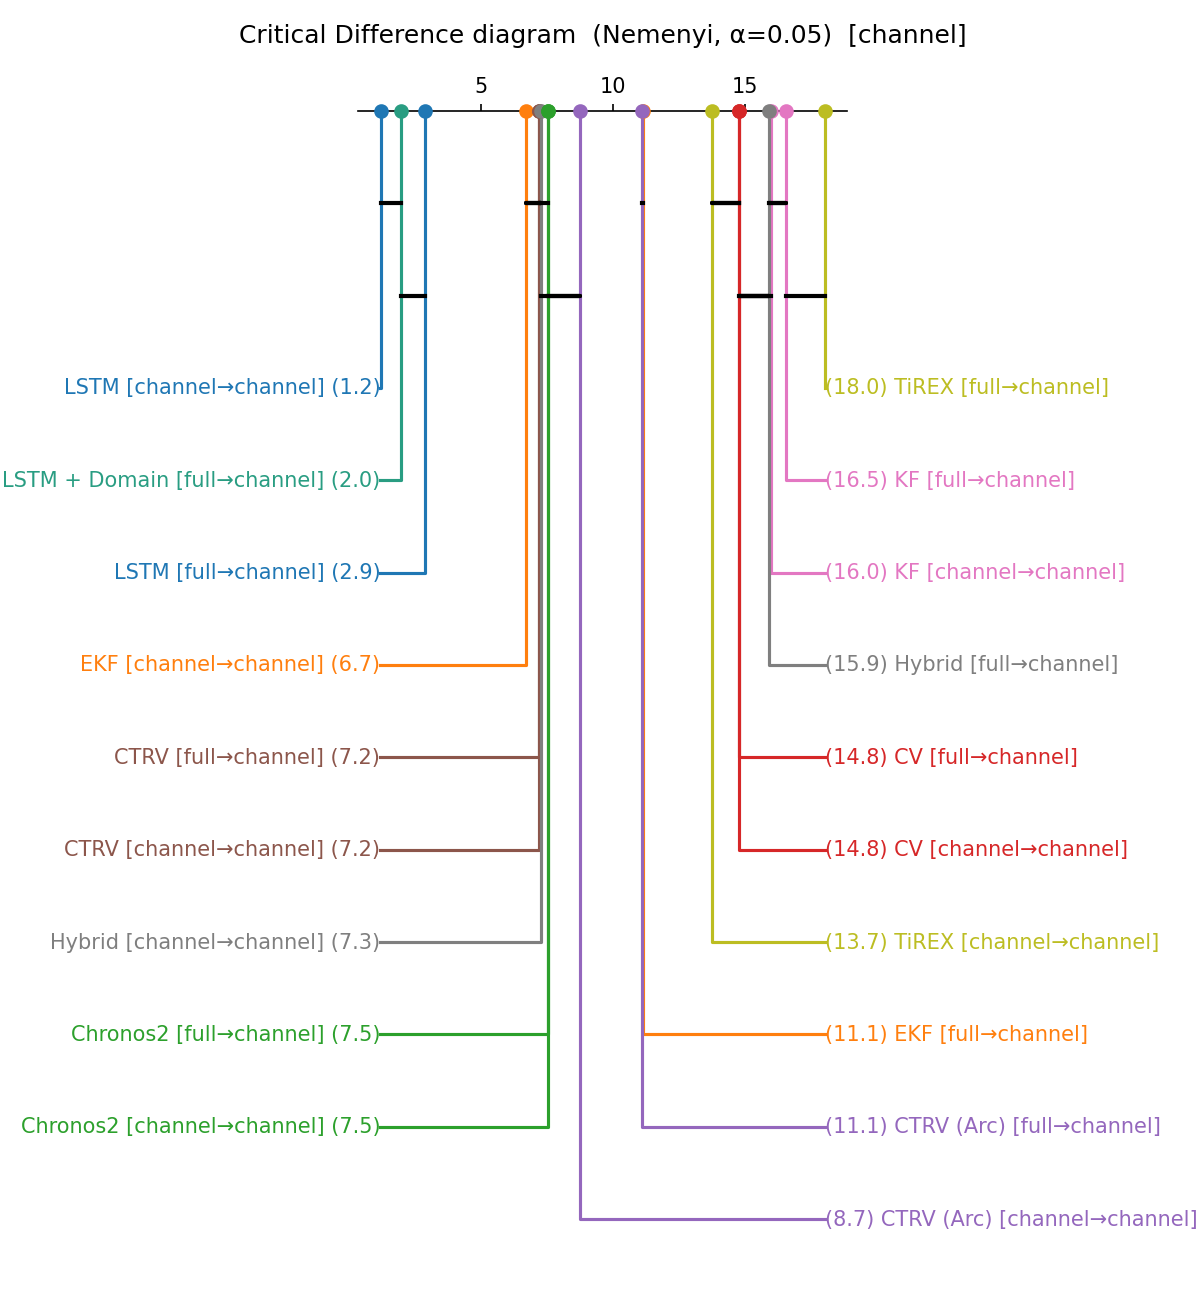
\includegraphics[height=0.48\textheight]{figures/cd_diagram_channel}\\[4pt]
    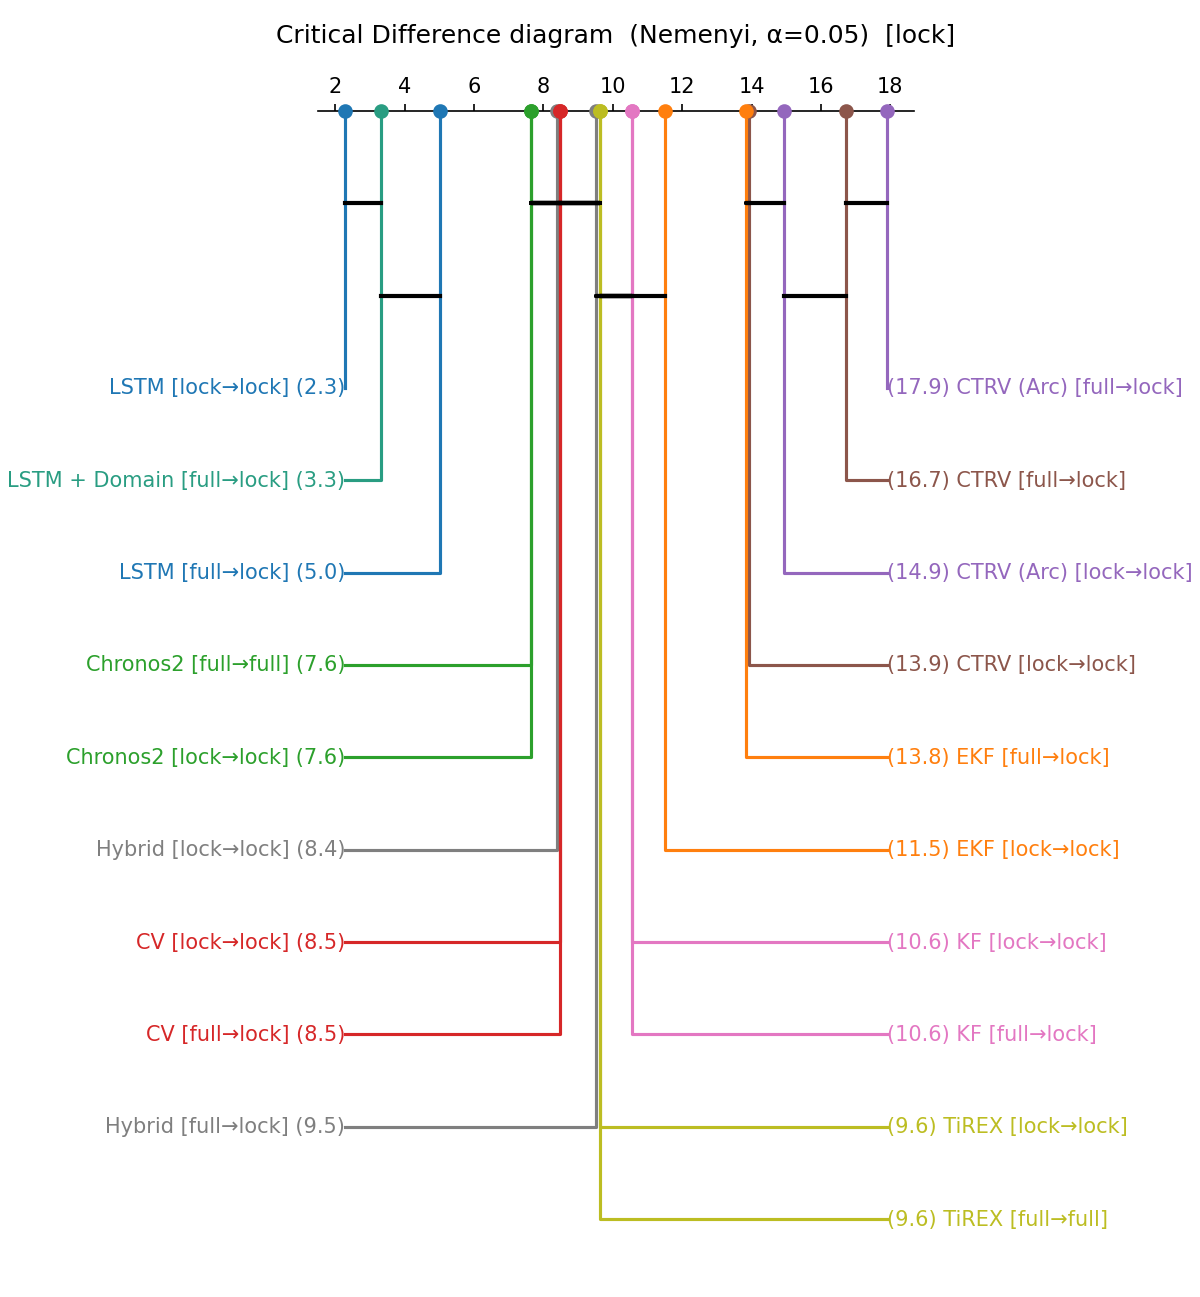
\includegraphics[height=0.48\textheight]{figures/cd_diagram_lock}
    \caption[Exp. II Friedman \& Nemenyi CD-Plots (1/2)]{\acf{CD} diagram based on the Friedman test and Nemenyi post-hoc comparison for mixed and domain specific training, evaluated per domain. Models connected by a horizontal bar are not significantly different at \( \alpha = 0.05\). The shown numbers are the mean rank per model in the evaluation, 1 being the best possible result. It can be observed that the harbour domain is the only environment where domain-specific training fails to produce a statistically significant improvement for the \ac{LSTM} (1/2).}
    \label{fig:cd-diagrams-a}
\end{figure}

% Seite 2: CD Diagrams 3–4
\begin{figure}[p]
    \ContinuedFloat
    \centering
    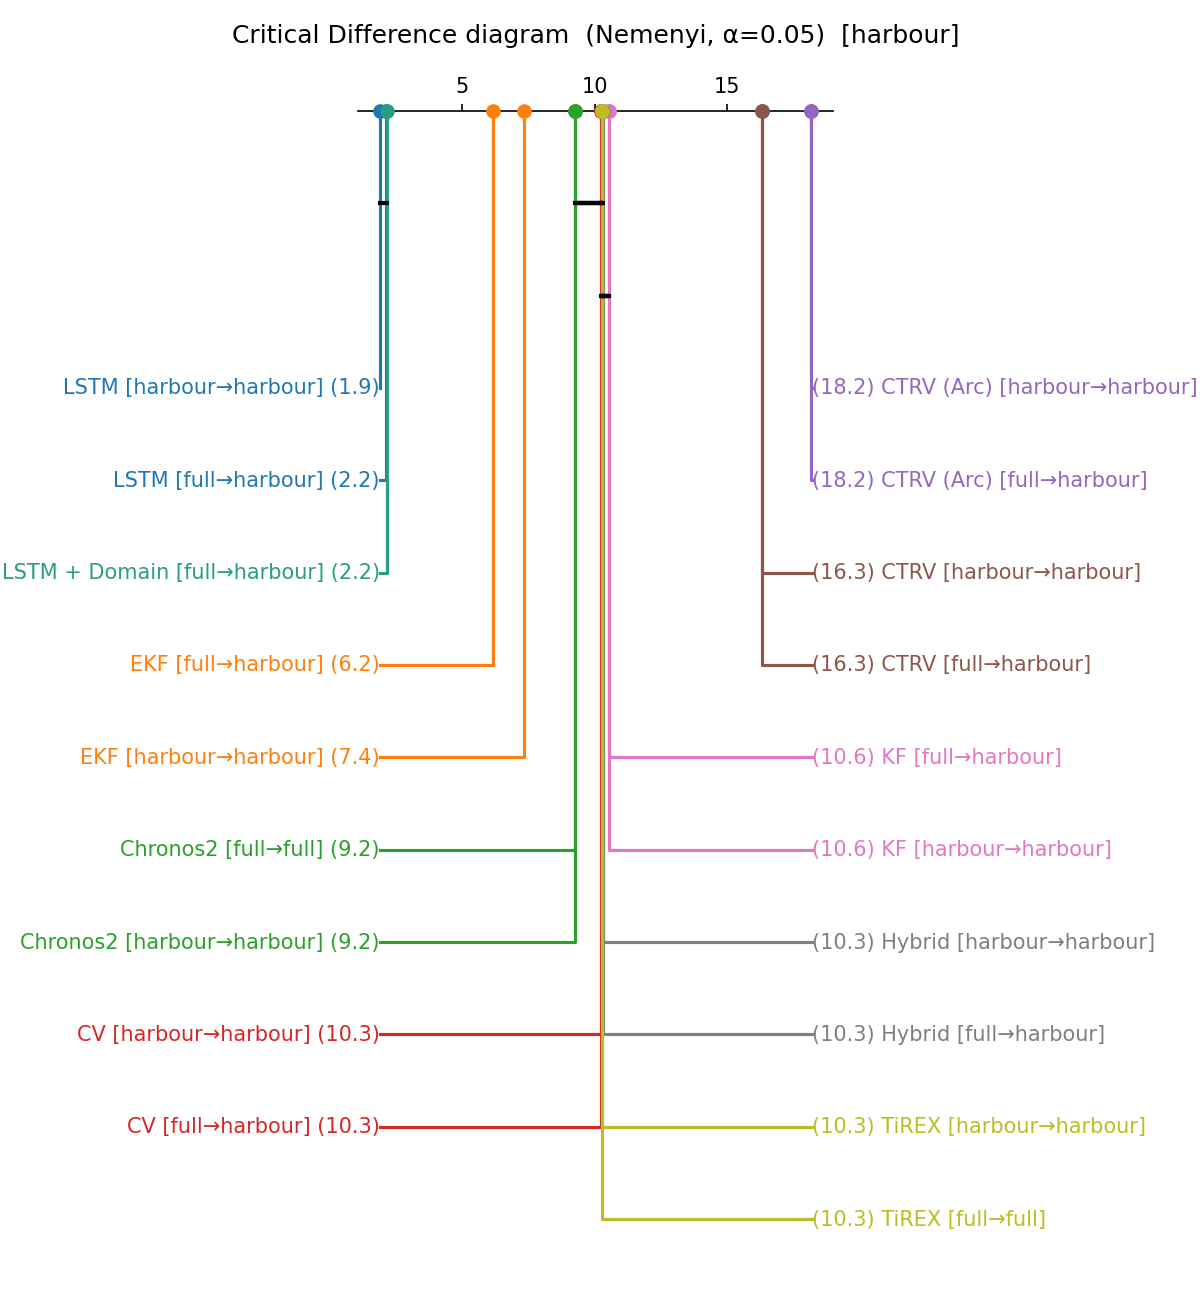
\includegraphics[height=0.48\textheight]{figures/cd_diagram_harbour}\\[4pt]
    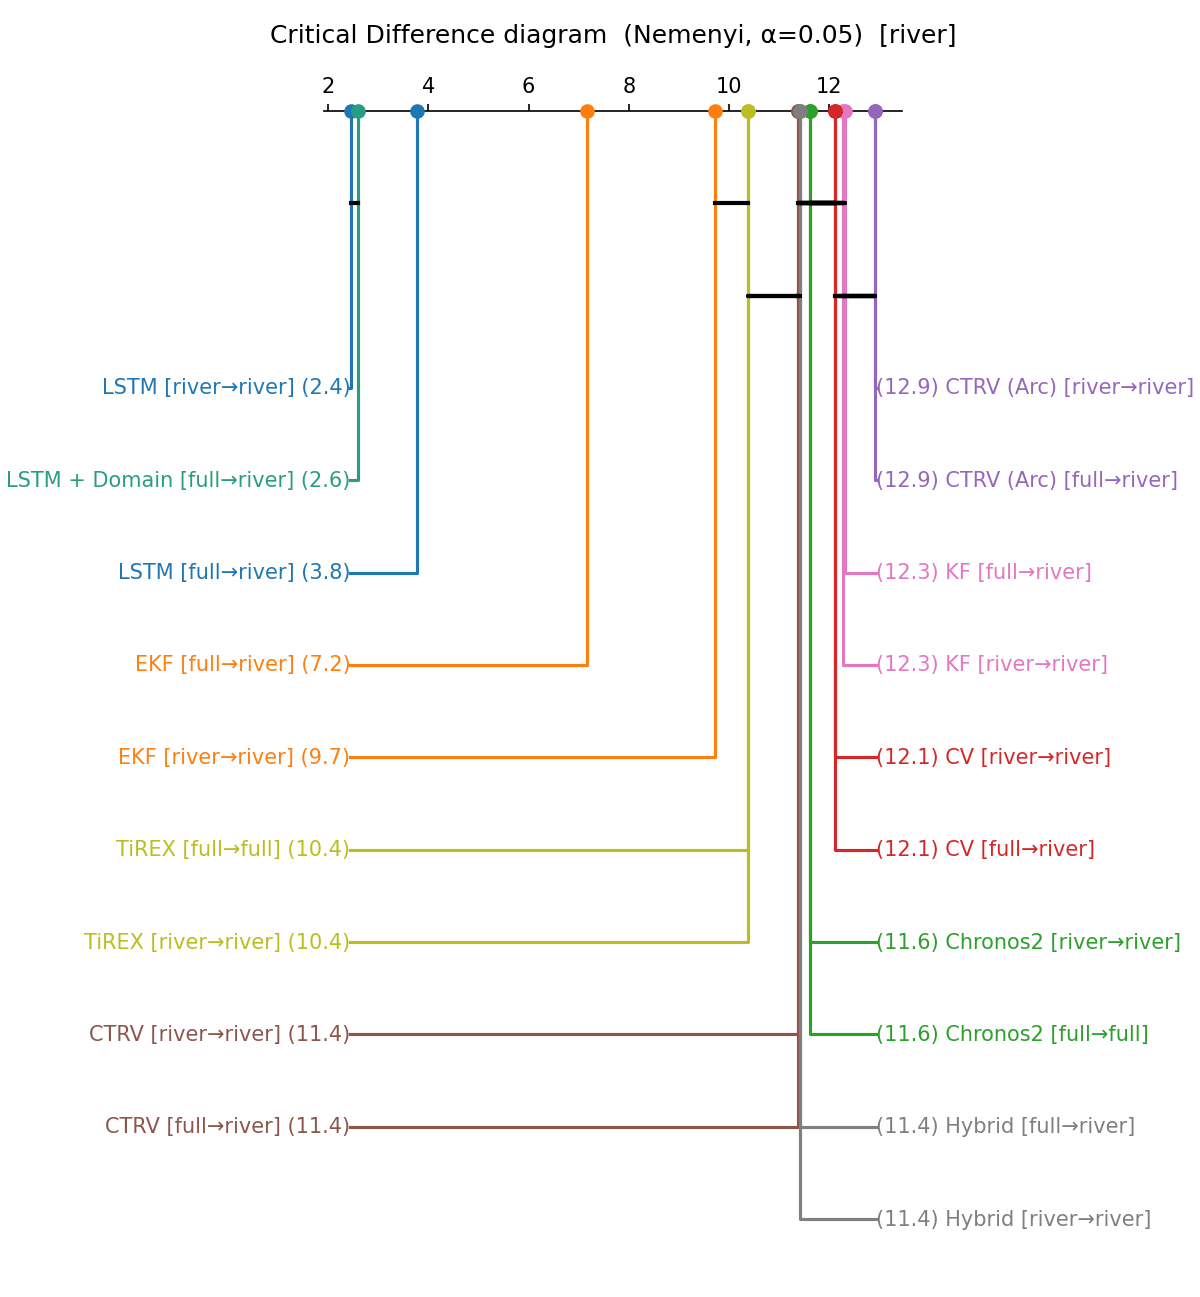
\includegraphics[height=0.48\textheight]{figures/cd_diagram_river}
    \caption[Exp. II Friedman \& Nemenyi CD-Plots (2/2)]{\acf{CD} diagram based on the Friedman test and Nemenyi post-hoc comparison for mixed and domain specific training, evaluated per domain. Models connected by a horizontal bar are not significantly different at \( \alpha = 0.05\). The shown numbers are the mean rank per model in the evaluation, 1 being the best possible result. It can be observed that the harbour domain is the only environment where domain-specific training fails to produce a statistically significant improvement for the \ac{LSTM} (2/2).}
    \label{fig:cd-diagrams-b}
\end{figure}

\begin{comment}
adjust caption if put in appendix again
    \begin{figure}
    \centering
    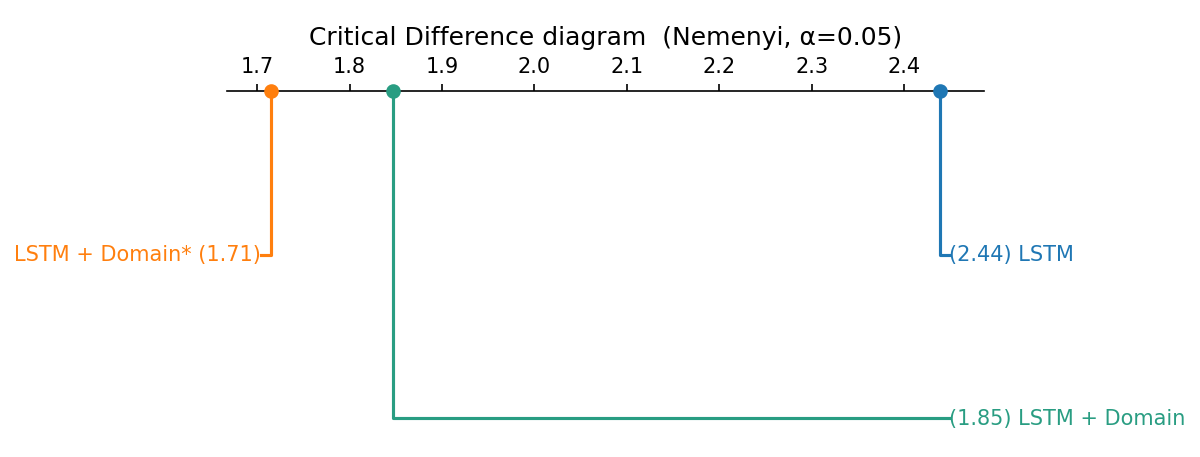
\includegraphics[width=0.75\linewidth]{figures/cd_diagram_lstm_comparison.png}
    \caption{Critical Difference Diagrams for LSTM domain encoding (mixed training and evaluation)}
    \label{fig:cd_exp3}
\end{figure}

\end{comment}






\FloatBarrier
\clearpage

\FloatBarrier

\chapter{Supplementary Tables} %unpassend
\label{appx:B}





\begin{table}[t]%%%%%%%%%%%% OPTIMiseR
    \centering
    %\caption{HPO Optimiser Configurations}
    \caption[Configuration Parameters for Optuna HPO]{Configuration parameters for the Optuna hyperparameter optimisation. The table details the specific search algorithms, trial counts, seeding strategies, and early stopping criteria applied to each model type, ranging from kinematic models to the LSTM.}
    \label{tab:hpo-config}
    \scalebox{1}{%  %% 5% smaller (0.95 = 95% of original size)

    \setlength{\tabcolsep}{4pt}  %% Reduce from default 6pt

    \begin{tabular}{ll}
        \toprule
        \textbf{Parameter} & \textbf{Value} \\
        \midrule
        \multicolumn{2}{l}{\textit{General}} \\
        HPO Framework       & Optuna \\ %\makecell[l]{Optuna (Grid Search for 1D HPO,\\TPE Sampler otherwise)} \\
        Device & CUDA (2 x RTX 4090) \\
        TPE Multivariate    & false \\
        Early Stopping Patience & 50 trials \\
        Early Stopping Min.\ Delta & $10^{-4}$ \\
        Random Seed & 42 \\

        \midrule
        \multicolumn{2}{l}{\textit{CV / CTRV / CTRV Arc}} \\
        Method              & Grid Search (1D) \\
        Search Space        & $ [1,\ \text{max}]$ \\
        \midrule
        \multicolumn{2}{l}{\textit{Hybrid CV/CTRV}} \\
        Method              & TPE \\
        Number of Trials    & 100 \\
        TPE Startup Trials  & 20 \\
        Seeded Initial Trial & CV/CTRV best \texttt{velocity\_steps} \\
        \midrule
        \multicolumn{2}{l}{\textit{Kalman Filter \& EKF}} \\
        Method              & TPE \\
        Number of Trials    & 100 \\
        TPE Startup Trials  & 20 \\
     
        \midrule
        \multicolumn{2}{l}{\textit{LSTM}} \\
        Method              & TPE + Successive Halving Pruner \\
        Number of Trials    & 100 \\
        TPE Startup Trials  & 26 (16 feature sets $+$ 10) \\
        Seeded Initial Trials & 16 (one per feature set) \\
        Pruner Min.\ Resource & 8 epochs \\
        Pruner Reduction Factor & 2 \\
        Pruner Min.\ Early Stopping Rate & 0 \\
        Max.\ Epochs        & 100 \\
        Training Patience   & 8 epochs \\
        Training Min.\ Delta & $10^{-4}$ \\
        \bottomrule
        \vspace{-2pt}
    \end{tabular}
    }%scalebox
\end{table}









    \begin{table}[t] %%%%%%---------- HP list - todo move to appendix if no space 
    \centering
    \caption[Model-specific Hyperparameters]{Model-specific hyperparameters used in the experiments.}
    \label{tab:model_hyperparameters}
    \begin{tabular}{ll}
    \toprule
    \textbf{Model} & \textbf{Hyperparameters} \\
    \midrule
    CV & $n_\text{vel}$ \\
    CTRV & $n_\text{vel}$ \\
    CTRV Arc & $n_\text{vel}$ \\
    Hybrid CV/CTRV & $n_\text{vel}^\text{CV}$, $n_\text{vel}^\text{CTRV}$, $n_\text{rot}$, $\tau_\text{rot}$ \\
    KF (CV) & $q_\text{pos}$, $q_\text{vel}$, $r_\text{pos}$, $p_{0,\text{pos}}$, $p_{0,\text{vel}}$ \\
    EKF (CTRV) & $q_\text{pos}$, $q_\text{vel}$, $q_\text{rot}$, $r_\text{pos}$, $p_{0,\text{pos}}$, $p_{0,\text{vel}}$, $p_{0,\text{rot}}$, $n_\text{ctx}$ \\
    Chronos-2 & -- \\
    TiREX & context length \\
    LSTM & hidden size, number of layers, dropout, learning rate, batch size, feature set \\
    LSTM + Domain & hidden size, number of layers, dropout, learning rate, batch size, feature set \\
    \bottomrule
    \end{tabular}
    \end{table} 





















%**************************************

\chapter{Methodological Details} 
\label{chap:appendixderivations}

\section{Mathematical Foundations of Sequence Models}
\label{appx: mathfoundations}
In this appendix, we present more details on the mathematical formalisations underlying the sequence models discussed in the main text.
\subsection*{\acf{RNN}}
Building on the first popular model to use recurrence, the Hopfield Network introduced by \textcite{hopfieldrnn}, the foundational concept for sequence-based learning is the \ac{RNN}. 
The primary distinction between \acp{RNN} and conventional Feedforward Neural Networks, such as \acp{MLP}, is the direction of information flow. 
While the latter are acyclic, \acp{RNN} use cycles to feed information back into the hidden state. 
With this architecture, the model incorporates context from previous inputs $X_{0:t-1}$ when processing the current input $X_t$, instead of processing each input in isolation \parencite{gentleschmidt2019recurrentneuralnetworksrnns}.
The basic structure of this recurrent process, configured as an Encoder-Decoder architecture, is illustrated in Figure~\ref{fig:s2s_rnn_appendix}.
Consequently, the network can make decisions based on the patterns it recognises \parencite{AIBook}. 
The recurrence can be expressed as Equation \ref{eq:app1},
\begin{equation}
    H_t = \phi_h (X_t W_{xh} + H_{t-1} W_{hh} + b_h) 
    \label{eq:app1}
\end{equation}
where $W$ represents weight matrices and $\phi$ an activation function. 
Despite their theoretical capability to handle sequences, \acp{RNN} suffer from the \emph{vanishing gradient problem}, as well as the \emph{exploding gradient problem}, as established by \textcite{279181bengio}.
As the sequence length increases, the gradients used to update weights during backpropagation decrease exponentially. 
This exponential decrease prevents the model from learning long-term dependencies.

\subsection*{\acf{LSTM}}
To address the limitations of standard \acp{RNN} to capture long-term dependencies, \textcite{hochreiterLSTM} introduced the \ac{LSTM} architecture. 
The corresponding archtiecture of the \ac{LSTM}-based Encoder-Decoder model is depicted in Figure~\ref{fig:s2s_lstm_appendix}.
The core innovation of the \ac{LSTM} is the introduction of a cell state $C_t$. 
Through this state, information persists across many time steps. 
The flow of information in and out of these cells is regulated by three gates:
\begin{itemize}
    \item \textbf{Forget Gate $F_t$}: Determines which information from the previous cell state $C_{t-1}$ is no longer needed and should be discarded.
    \item \textbf{Input Gate $I_t$}: Decides which new information from the current input $X_t$ and previous hidden state $H_{t-1}$ is relevant to be stored in the cell state.
    \item \textbf{Output Gate $O_t$}: Controls which parts of the current cell state $C_t$ are used to compute the new hidden state $H_t$.
\end{itemize}

Following the formalisation by \textcite{gentleschmidt2019recurrentneuralnetworksrnns}, the internal update process can be defined by Equation~\ref{eq:lstm_updates}:
\begin{equation}
    \begin{aligned}
        F_t &= \sigma(X_t W_{xf} + H_{t-1} W_{hf} + b_f), \\
        I_t &= \sigma(X_t W_{xi} + H_{t-1} W_{hi} + b_i), \\
        \tilde{C}_t &= \tanh(X_t W_{xc} + H_{t-1} W_{hc} + b_c), \\
        C_t &= F_t \odot C_{t-1} + I_t \odot \tilde{C}_t, \\
        O_t &= \sigma(X_t W_{xo} + H_{t-1} W_{ho} + b_o), \\
        H_t &= O_t \odot \tanh(C_t).
    \end{aligned}
    \label{eq:lstm_updates}
\end{equation}

In these equations, $\tilde{C}_t$ represents a candidate cell state, $\sigma$ is the sigmoid activation function $\sigma(x) = \frac{1}{1 + e^{-x}}$, and $\odot$ denotes the element-wise (Hadamard) product.
$W$ and $b$ are the respective weights and biases.
This update procedure for the cell state $C_t$ prevents the gradient from vanishing as quickly as in standard \acp{RNN}.

As indicated by the multi-dimensional input vector $X_t$ and the associated weight matrices, the \ac{LSTM} architecture is mathematically equipped for multivariate sequence modelling. 
The model has the capacity to represent nonlinear cross-channel correlations, because the internal gating mechanisms integrate information from all input features simultaneously.
This integration models their interdependencies within a shared hidden representation.
Consequently, this design is highly suitable for the present use case.

\begin{figure}[htbp]
    \centering
    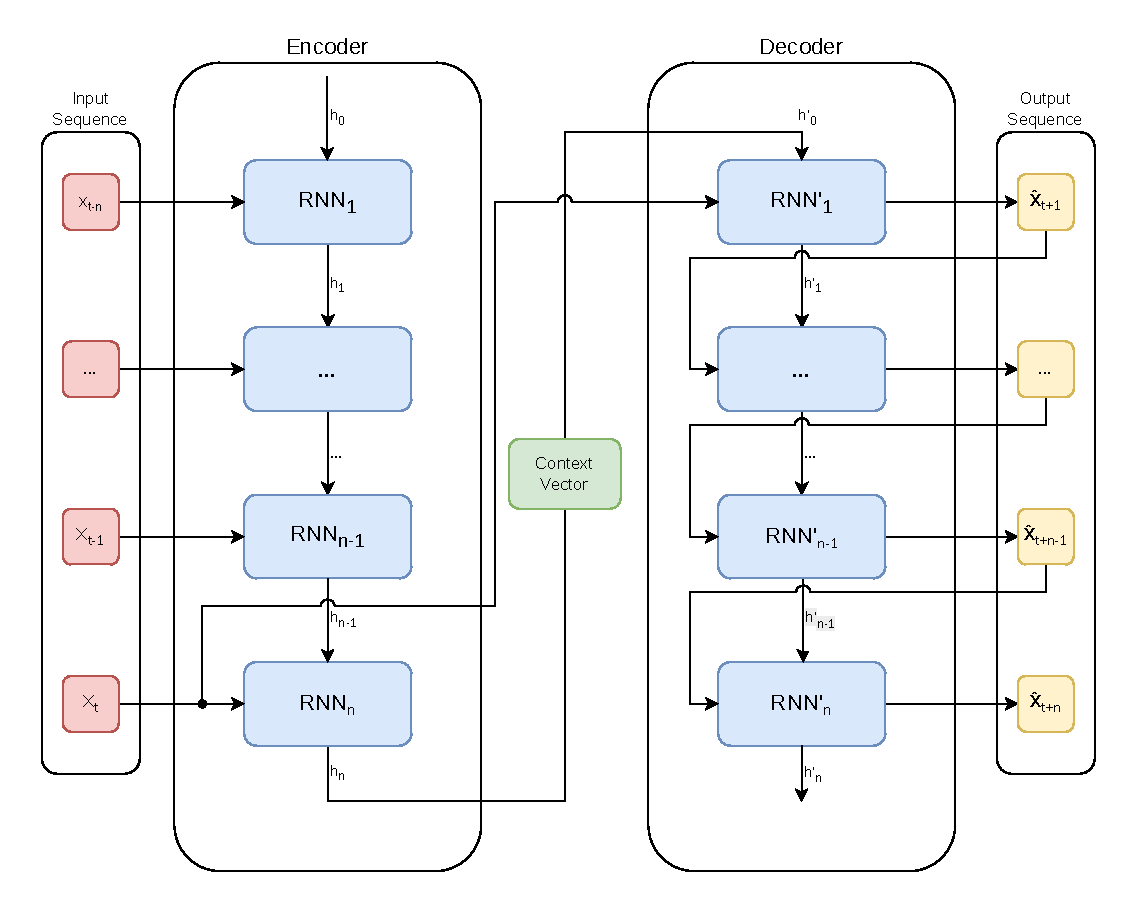
\includegraphics[width=0.75\linewidth]{figures/S2S_RNN.drawio (1).pdf}
    \caption[RNN Architecture]{Architecture of the standard \acf{RNN} Encoder-Decoder model (1 Layer).}
    \label{fig:s2s_rnn_appendix}
\end{figure}

\begin{figure}[htbp]
    \centering
    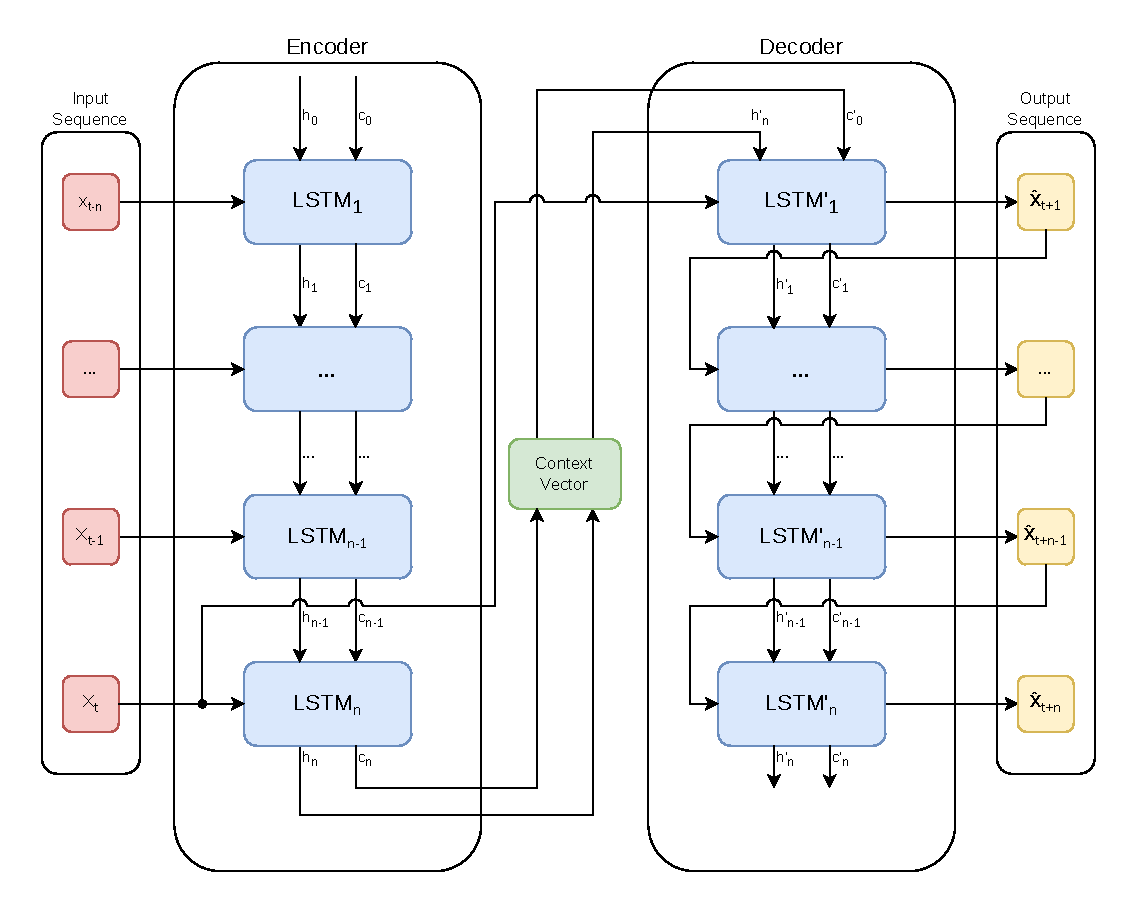
\includegraphics[width=0.75\linewidth]{figures/S2S_LSTM.drawio (1).pdf}
    \caption[LSTM Architecture]{Architecture of the \acf{LSTM} Encoder-Decoder model (1 Layer).}
    \label{fig:s2s_lstm_appendix}
\end{figure}

\newpage % bled into the middle of BO TPE text

\section{Bayesian Optimisation and the Tree-Parzen-Estimator}
\label{appx:BOandTPE}



In \acf{BO}, past evaluations are used to make informed decisions about which hyperparameters to test next.
This approach is critical for models where evaluating the true objective function $\mathcal{L}$ is computationally expensive (e.g., when fully training an \ac{LSTM}) \parencite{hutter2019automated}.
In \ac{BO}, this is achieved by constructing a probabilistic surrogate model $\hat{f}$, which approximates the true, expensive loss function based on all previously evaluated configurations.
Because the surrogate model $\hat{f}$ is computationally cheap to evaluate, more potential configurations can be tested to identify the most promising candidates before resources are committed to a full model training.

To decide which configuration to evaluate next based on the given surrogate model, an acquisition function is utilised.
A commonly applied acquisition function is \acf{EI} \parencite{AutoMLHoos}.
In \ac{EI}, a candidate is evaluated by combining two essential terms: the expected value of the function at a given point, and the associated variance.
This combination provides a trade-off between two competing goals:

\begin{itemize}
    \item \textbf{Exploitation:} By considering the expected value, the search is focused on promising regions of the search space that contain good candidate solutions with high probability.
    \item \textbf{Exploration:} In contrast, the variance term encourages the exploration of unknown areas that are weakly explored, or where candidate solutions of highly variable quality have been observed \parencite{Jones1998}.
\end{itemize}
Figure~\ref{fig:bo_illustration} illustrates one iteration of this process. %published as open acces. Open access works published by Springer Nature are published under Creative Commons licences.tdoo resolved (check licensing, otherwise use the one from the literature overview automl timeseries)

\begin{figure} [h]
    \centering
    % Adjust trim values (left bottom right top) 
    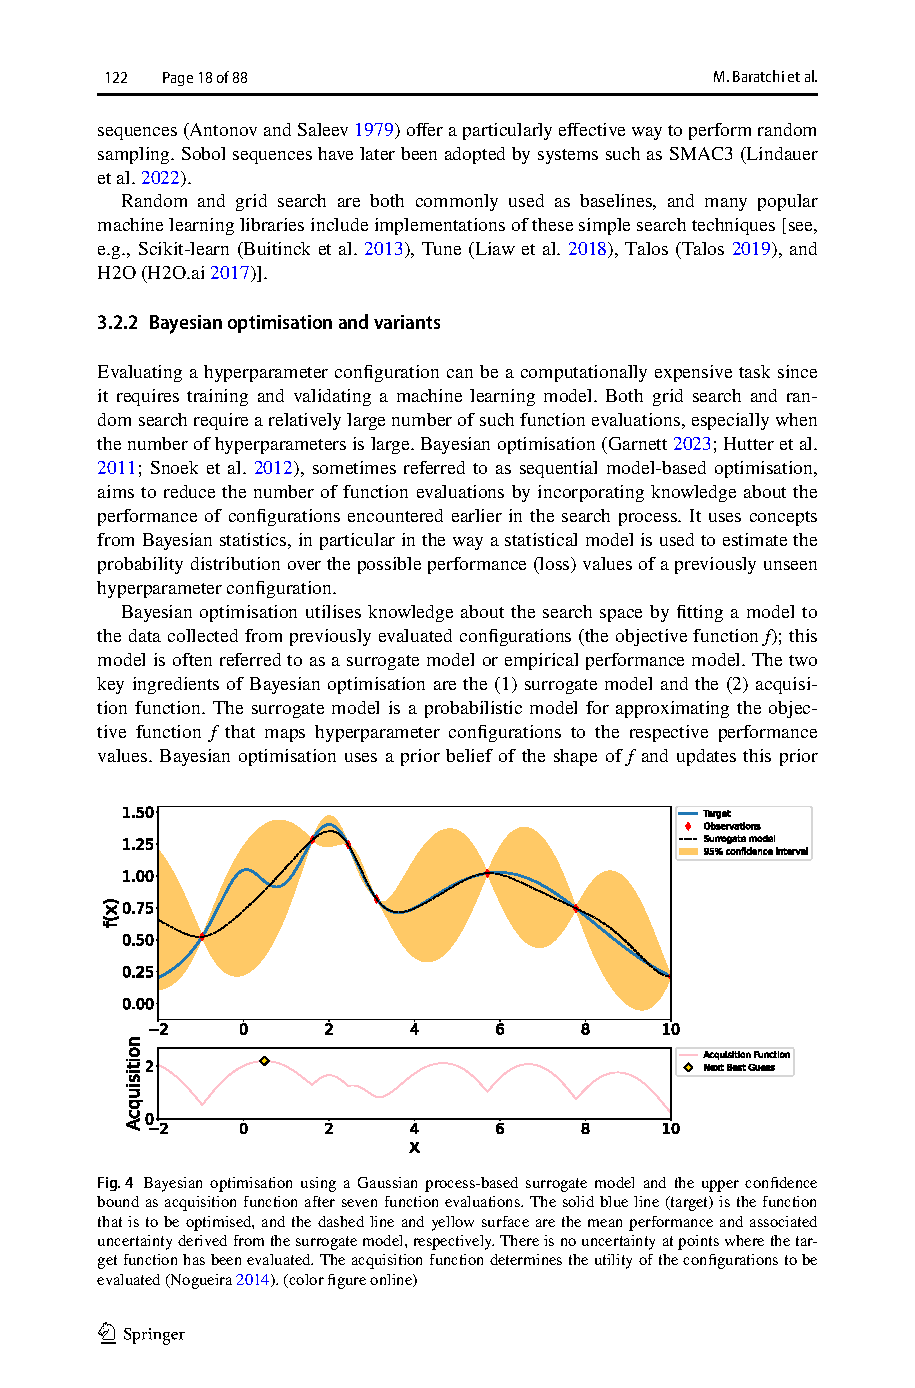
\includegraphics[width=0.9\linewidth,trim={2cm 4cm 2cm 13.5cm}, clip]{figures/985693BO.pdf}
    \caption[Bayesian Optimisation]{\acf{BO} using a surrogate model and \acf{EI} after several evaluations. The solid line represents the true objective $\mathcal{L}$, the dashed line and shaded region show the surrogate mean and 95\% confidence interval, respectively. The acquisition function (bottom) determines the next candidate configuration to evaluate \parencite{AutoMLHoos}.}
    \label{fig:bo_illustration}
\end{figure}

While classical \ac{BO} surrogate models, such as Gaussian Processes, model $p(y \mid \lambda)$ directly, they scale poorly with the number of hyperparameters and struggle with discrete and categorical parameters \cite{AutoMLHoos}.
To address these limitations, the modelling problem is inverted in the \acf{TPE} algorithm \parencite{bergstra2011algorithms}.
Rather than directly modelling $p(y \mid \lambda)$, two separate density functions, $p(\lambda \mid y < \alpha)$ and $p(\lambda \mid y \geq \alpha)$, are constructed in the \ac{TPE}.
With the threshold $\alpha$, all observations are partitioned into a set of good and bad configurations, each of which is modelled using one-dimensional Parzen windows.
Parzen windows are kernel density estimators that place a smooth Gaussian function at each data point, with their sum forming the density function.
The ratio $\frac{p(\lambda \mid y \ge \alpha)}{p(\lambda \mid y < \alpha)}$ is closely related to the \ac{EI} acquisition function and serves as the criterion for proposing new hyperparameter configurations \parencite{bergstra2011algorithms, hutter2019automated}.
Figure~\ref{fig:tpe_illustration} illustrates this partitioning and selection process.

\begin{figure}[h]
    \centering
    % Insert the TPE figure created for the defence here
    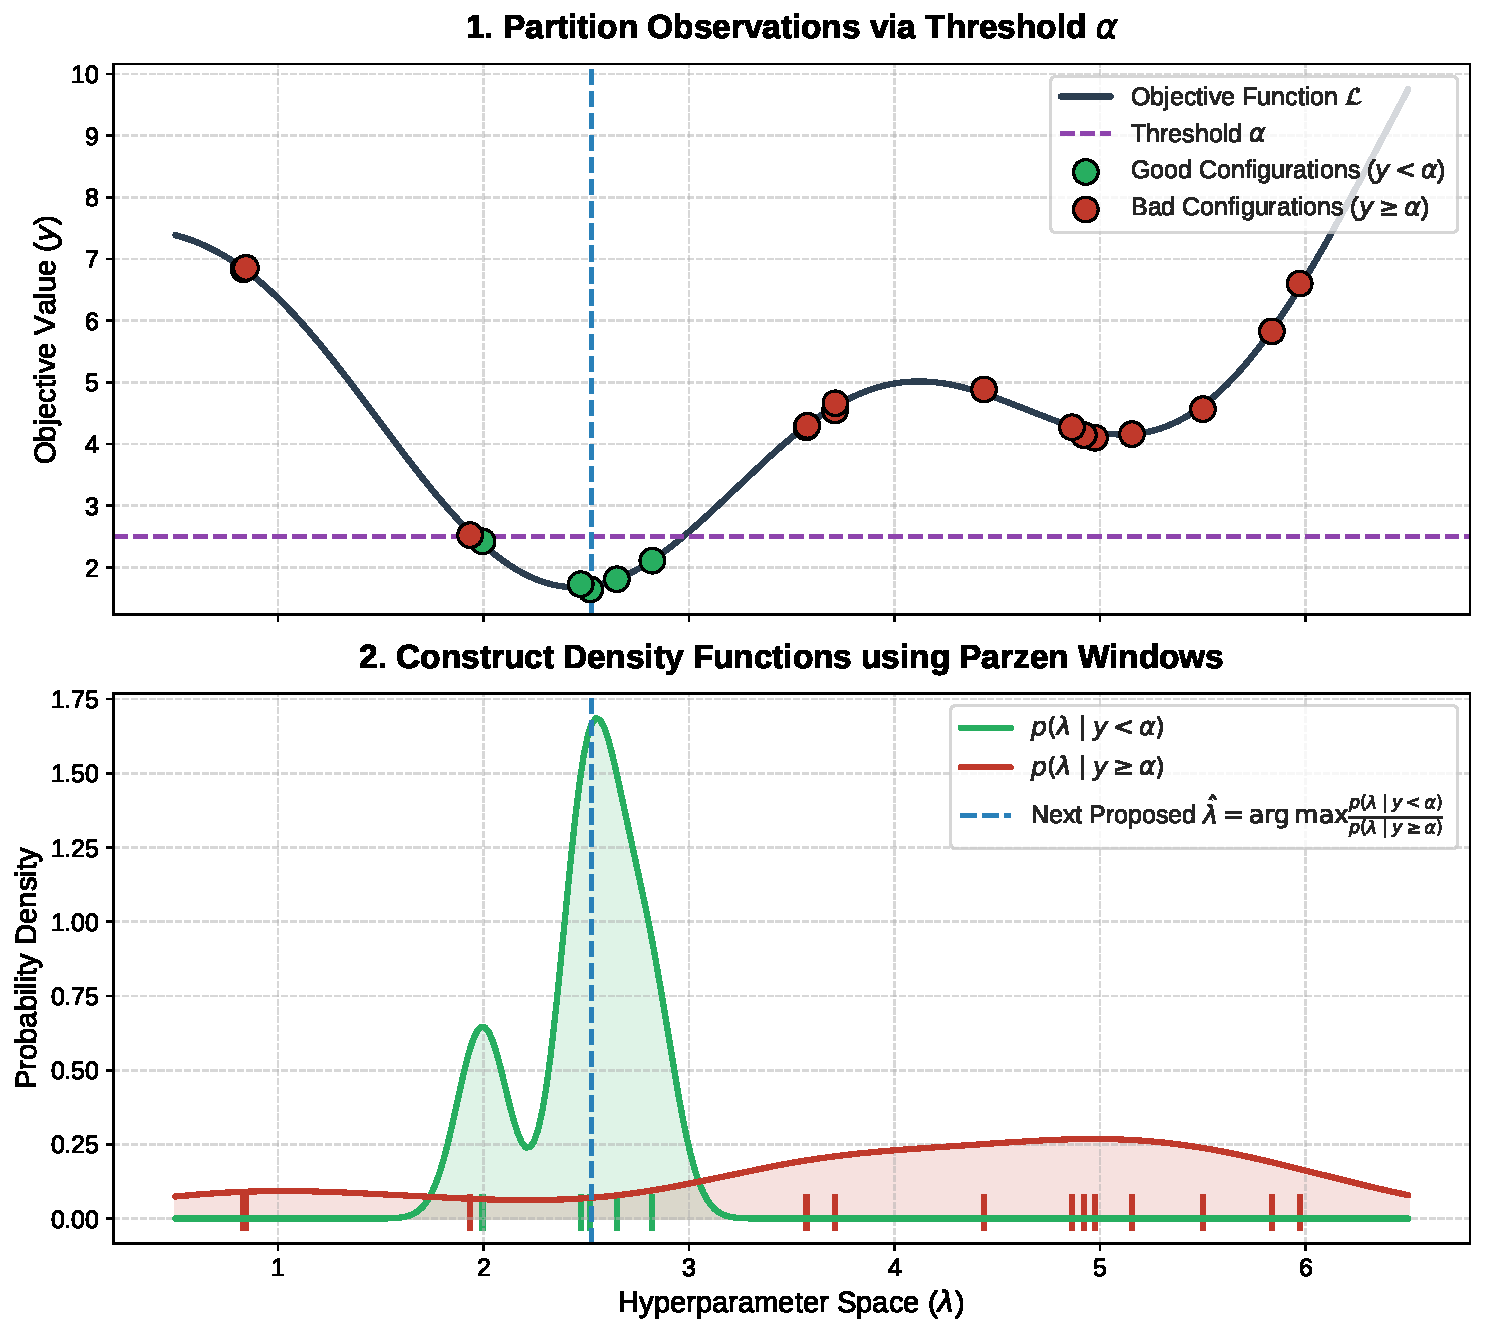
\includegraphics[width=0.8\linewidth]{figures/tpe_mathematical_mechanism.pdf}
\caption[Tree-structured Parzen Estimator]{Mathematical mechanism of the \acf{TPE}. The upper window illustrates the objective function $\mathcal{L}$, where evaluated configurations are partitioned by the threshold $\alpha$. Green points represent promising configurations falling below this threshold, whereas red points indicate suboptimal configurations. The lower window displays the corresponding probability density functions constructed using Parzen windows: $p(\lambda \mid y < \alpha)$ for the good configurations and $p(\lambda \mid y \ge \alpha)$ for the bad configurations. The next hyperparameter configuration to be evaluated is proposed based on these distributions, indicated by the vertical blue dashed line across both plots.}
\label{fig:tpe_illustration}
\end{figure}

\FloatBarrier

\section{Mathematical Details of the Search Space}
\label{app:math_search_space}

This appendix provides the formal mathematical definitions for the \ac{AutoML} search space components introduced in Section \ref{subsec:search_space}.
All definitions are adapted from \textcite{AutoMLHoos} to reflect the fixed training and validation split we used for this work.

\paragraph{Hyperparameter Optimisation.}

Let $A_{\lambda}$ denote a learning algorithm $A$ instantiated with hyperparameter configuration $\lambda \in \Lambda$, where $\Lambda$ is the hyperparameter search space.
Given a dataset $\mathcal{D}$ split into a training set $\mathcal{D}_{train}$ and a validation set $\mathcal{D}_{val}$, the \ac{HPO} objective is defined as Equation \ref{eq:app8},
\begin{equation}
    \lambda^* = \arg\min_{\lambda \in \Lambda} \mathcal{L}(A_{\lambda}, \mathcal{D}_{train}, \mathcal{D}_{val})
    \label{eq:app8}
\end{equation}
where $\mathcal{L}$ represents a validation loss metric. Since evaluating $\mathcal{L}$ requires fully training $A_\lambda$, each function evaluation is expensive, and \ac{HPO} is a black-box optimisation problem.

\paragraph{Model Selection.}
The algorithm selection problem is defined as finding the algorithm $A^* \in \mathcal{A}$ that yields the lowest error on the validation set, as defined per Equation \ref{eq:appx9}.
\begin{equation}
    A^* = \arg\min_{A \in \mathcal{A}} \mathcal{L}(A, \mathcal{D}_{train}, \mathcal{D}_{val})
    \label{eq:appx9}
\end{equation}

\paragraph{CASH Problem.}
Given a set of learning algorithms $\mathcal{A}$, each algorithm $A^{(j)} \in \mathcal{A}$ is associated with a specific hyperparameter configuration space $\Lambda^{(j)}$.
The \ac{CASH} problem is formulated to jointly identify the optimal algorithm $A^*$ and its corresponding optimal hyperparameter configuration $\lambda^*$, as defined per Equation \ref{eq:appx10}:
\begin{equation}
    A^*, \lambda^* = \arg\min_{A^{(j)} \in \mathcal{A}, \lambda \in \Lambda^{(j)}} \mathcal{L}(A^{(j)}_{\lambda}, \mathcal{D}_{train}, \mathcal{D}_{val})
    \label{eq:appx10}
\end{equation}





\FloatBarrier









\section{CTRV--EKF Jacobian Derivation}
\label{app:ctrv-jacobian}

This appendix derives the full Jacobian $\mathbf{A}_k = \partial f /
\partial \mathbf{x}|_{\hat{\mathbf{x}}^+_k}$ of the CTRV transition
function introduced in Eq.~\eqref{eq:ctrv-ekf-f_and_c}. 
The state vector is $\hat{\mathbf{x}}_k = (x_k,\, y_k,\, \dot{x}_k,\, \dot{y}_k,\, \omega_k)^\top$ and $\Delta\psi = \omega_k\,\Delta t$.

\subsection*{Case $|\omega_k| \geq \varepsilon$}

\paragraph{Position rows with respect to $(x_k, y_k)$.}
The new position $x_{k+1} = x_k + g(\dot{x}_k, \dot{y}_k, \omega_k)$ depends on $x_k$
linearly with slope 1, and does not depend on $y_k$. The partial derivatives are defined by Equation~\ref{eq:deriv_pos_xy}.
\begin{equation}
    \frac{\partial x_{k+1}}{\partial x_k} = 1, \quad
    \frac{\partial x_{k+1}}{\partial y_k} = 0, \quad
    \frac{\partial y_{k+1}}{\partial x_k} = 0, \quad
    \frac{\partial y_{k+1}}{\partial y_k} = 1
    \label{eq:deriv_pos_xy}
\end{equation}

\paragraph{Position rows with respect to $(\dot{x}_k, \dot{y}_k)$.}
The arc-length update is given by Equation~\ref{eq:arclength_update}:
\begin{equation}
    x_{k+1} = x_k + \frac{\dot{x}_k\sin\Delta\psi + \dot{y}_k(\cos\Delta\psi - 1)}{\omega_k},\quad
    y_{k+1} = y_k + \frac{\dot{y}_k\sin\Delta\psi - \dot{x}_k(\cos\Delta\psi - 1)}{\omega_k}
    \label{eq:arclength_update}
\end{equation}


 Because both terms appear linearly, differentiation with respect to $\dot{x}_k$ and $\dot{y}_k$ yields Equation~\ref{eq:deriv_pos_vel},:
\begin{equation}
    \frac{\partial x_{k+1}}{\partial \dot{x}_k} = \frac{\sin\Delta\psi}{\omega_k}, \quad
    \frac{\partial x_{k+1}}{\partial \dot{y}_k} = \frac{\cos\Delta\psi - 1}{\omega_k}, \quad
    \frac{\partial y_{k+1}}{\partial \dot{x}_k} = \frac{1 - \cos\Delta\psi}{\omega_k}, \quad
    \frac{\partial y_{k+1}}{\partial \dot{y}_k} = \frac{\sin\Delta\psi}{\omega_k}
    \label{eq:deriv_pos_vel}
\end{equation}

\paragraph{Position rows with respect to $\omega_k$.}
By applying the quotient rule to $x_{k+1} = x_k + u(\omega_k)/\omega_k$, where $u = \dot{x}_k\sin\Delta\psi + \dot{y}_k(\cos\Delta\psi - 1)$ and $\mathrm{d}\Delta\psi/\mathrm{d}\omega_k = \Delta t$, the derivative is obtained as shown in Equation~\ref{eq:deriv_pos_omega}.
\begin{align}
    \frac{\partial x_{k+1}}{\partial \omega_k}
    &= \frac{\omega_k \cdot \frac{\mathrm{d}u}{\mathrm{d}\omega_k} - u}{\omega_k^2}
     = \frac{\Delta t\,(\dot{x}_k\cos\Delta\psi - \dot{y}_k\sin\Delta\psi)\cdot\omega_k
             - \bigl(\dot{x}_k\sin\Delta\psi + \dot{y}_k(\cos\Delta\psi-1)\bigr)}{\omega_k^2}
    \label{eq:deriv_pos_omega}
\end{align}
The numerator factor $\dot{x}_k\cos\Delta\psi - \dot{y}_k\sin\Delta\psi$ corresponds to the rotated velocity $\dot{x}_{k+1}$ from $f$, which results in the compact form defined by Equation~\ref{eq:a15}:
\begin{equation}
    a_{15} = \frac{\Delta\psi\,\dot{x}_{k+1} - \bigl(\dot{x}_k\sin\Delta\psi + \dot{y}_k(\cos\Delta\psi-1)\bigr)}{\omega_k^2}
    \label{eq:a15}
\end{equation}
Analogously, the derivation for $a_{25}$ yields Equation~\ref{eq:a25}:
\begin{equation}
    a_{25} = \frac{\Delta\psi\,\dot{y}_{k+1} - \bigl(\dot{y}_k\sin\Delta\psi - \dot{x}_k(\cos\Delta\psi-1)\bigr)}{\omega_k^2}
    \label{eq:a25}
\end{equation}



\paragraph{Velocity rows with respect to $(\dot{x}_k, \dot{y}_k)$.}
The velocity update is a rotation by $\Delta\psi$, represented by Equation~\ref{eq:vel_rot_mat}.
\begin{equation}
    \begin{pmatrix}\dot{x}_{k+1}\\\dot{y}_{k+1}\end{pmatrix} = \mathbf{R}(\Delta\psi) \begin{pmatrix}\dot{x}_k\\\dot{y}_k\end{pmatrix}, \quad
    \mathbf{R}(\Delta\psi) = \begin{pmatrix}\cos\Delta\psi & -\sin\Delta\psi \\ \sin\Delta\psi &  \cos\Delta\psi\end{pmatrix}
    \label{eq:vel_rot_mat}
\end{equation}
Since the update is linear in $(\dot{x}_k, \dot{y}_k)$, the Jacobian block is
$\mathbf{R}(\Delta\psi)$ itself.

\paragraph{Velocity rows with respect to $\omega_k$.}
Differentiating $\dot{x}_{k+1} = \dot{x}_k\cos\Delta\psi - \dot{y}_k\sin\Delta\psi$
with respect to $\omega_k$, using $\mathrm{d}\Delta\psi/\mathrm{d}\omega_k = \Delta t$, results in Equation~\ref{eq:vel_deriv_omega}.
\begin{equation}
    \frac{\partial \dot{x}_{k+1}}{\partial \omega_k} =
    (-\dot{x}_k\sin\Delta\psi - \dot{y}_k\cos\Delta\psi)\,\Delta t, \qquad
    \frac{\partial \dot{y}_{k+1}}{\partial \omega_k} =
    (\dot{x}_k\cos\Delta\psi - \dot{y}_k\sin\Delta\psi)\,\Delta t
        \label{eq:vel_deriv_omega}
\end{equation}


\paragraph{Turn-rate row.}
Since $\omega_{k+1} = \omega_k$, all partial derivatives are zero except
$\partial\omega_{k+1}/\partial\omega_k = 1$.

\subsection*{Case $|\omega_k| < \varepsilon$: Taylor Approximation}

To avoid division by zero, we substitute:
\begin{equation}
    \sin\Delta\psi \approx \Delta\psi, \qquad
    \cos\Delta\psi \approx 1.
\end{equation}

To avoid division by zero, we apply the Taylor approximations as defined by Equation~\ref{eq:taylor_approx}.
\begin{equation}
    \sin\Delta\psi \approx \Delta\psi, \qquad \cos\Delta\psi \approx 1.
    \label{eq:taylor_approx}
\end{equation}

The position update simplifies to the constant-velocity step
$x_{k+1} \approx x_k + \dot{x}_k\,\Delta t$, $y_{k+1} \approx y_k + \dot{y}_k\,\Delta t$,
while the Jacobian is reduced to the form defined by Equation~\ref{eq:jacobian_taylor}.


\begin{equation}
    \mathbf{A}_k\big|_{|\omega_k|<\varepsilon} =
    \begin{pmatrix}
        1 & 0 & \Delta t & 0 & -\tfrac{1}{2}\dot{y}_k\,\Delta t^2 \\
        0 & 1 & 0 & \Delta t &  \tfrac{1}{2}\dot{x}_k\,\Delta t^2 \\
        0 & 0 & 1 & 0 & -\dot{y}_k\,\Delta t \\
        0 & 0 & 0 & 1 &  \dot{x}_k\,\Delta t \\
        0 & 0 & 0 & 0 & 1
    \end{pmatrix}
    \label{eq:jacobian_taylor}
\end{equation}


%%%%%%%%%%%%%----------------%%%%%%%%%%%%%%%%%%%%----------------------------------CODEBASE--------------------%%%%%%%%%%%%%%%%%%%%%%%%%%%%%%%%%%%%%%%%%%%%%%%%
\chapter{Codebase Overview} 
\label{chap:appendixcodebase}


\begin{figure}[p]
    \centering
    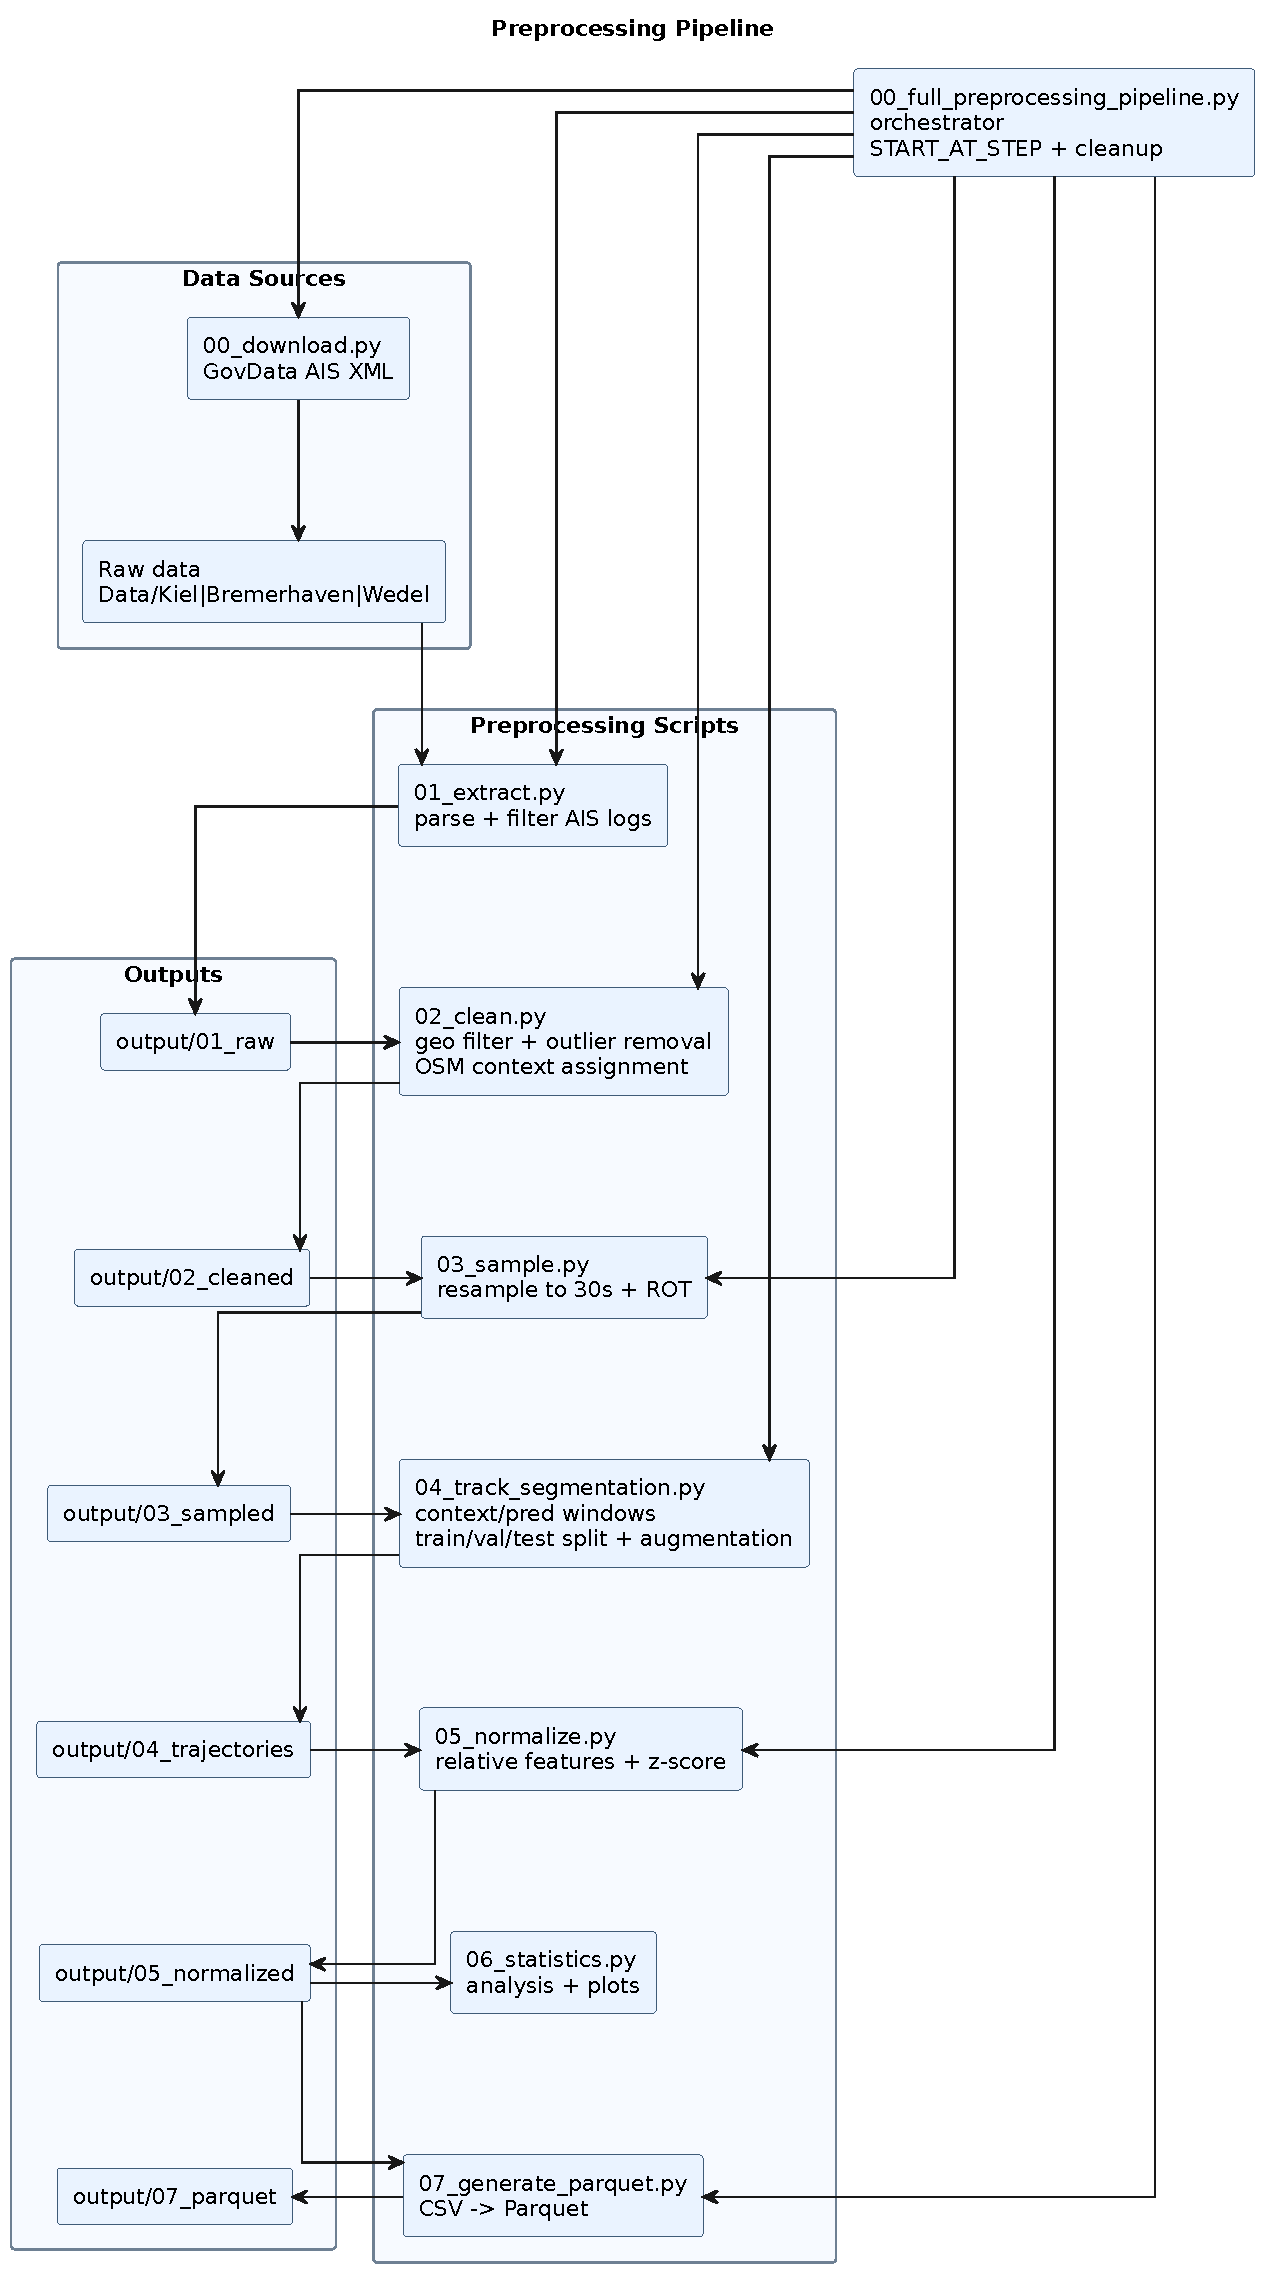
\includegraphics[width=0.75\linewidth]{figures/preprocessing_highlevel.pdf}
    \caption[Code Overview: Preprocessing Pipeline]{%
    \textbf{Preprocessing pipeline file interactions.}
    The pipeline is orchestrated by \texttt{00\_full\_preprocessing\_pipeline.py}, which invokes steps 01--07 sequentially and can resume from any intermediate step via \texttt{START\_AT\_STEP}.
    Raw AIS data is fetched by \texttt{00\_download.py} and stored under \texttt{Data/}.
    Each script reads from the previous output folder and writes into the next:
    \texttt{01\_extract.py} $\to$ \texttt{output/01\_raw} $\to$
    \texttt{02\_clean.py} $\to$ \texttt{output/02\_cleaned} $\to$
    \texttt{03\_sample.py} $\to$ \texttt{output/03\_sampled} $\to$
    \texttt{04\_track\_segmentation.py} $\to$ \texttt{output/04\_trajectories} $\to$
    \texttt{05\_normalize.py} $\to$ \texttt{output/05\_normalized} $\to$
    \texttt{07\_generate\_parquet.py} $\to$ \texttt{output/07\_parquet}.
    \texttt{06\_statistics.py} reads from \texttt{output/05\_normalized} to generate analysis figures and produces no further output folder.

    }    \label{fig:codepreprocessing}
\end{figure}

\clearpage


\begin{sidewaysfigure}
    \centering
    \makebox[0pt]{%symetrical overflow
        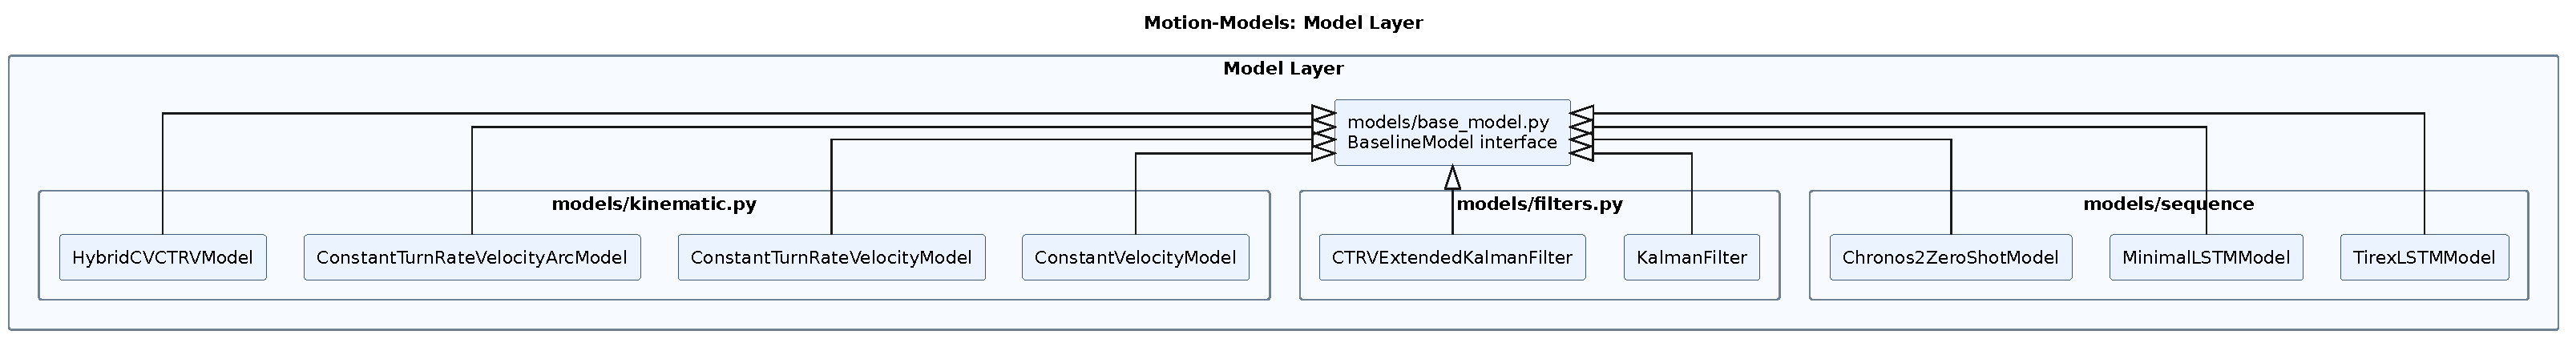
\includegraphics[width=1.18\textheight, keepaspectratio]{figures/models_highlevel.pdf}
    }
    \caption[Code Overview: Model Layer]{%
        \textbf{Model layer class hierarchy.}
        All models inherit from \texttt{BaselineModel} (\texttt{models/base\_model.py}), which defines the common interface used by the evaluation framework: \texttt{predict(context\_df,~n\_pred\_steps)}.
        The \emph{kinematic} group (\texttt{models/kinematic.py}) contains: \texttt{ConstantVelocityModel} (CV), \texttt{ConstantTurnRateVelocityModel} (CTRV), \texttt{ConstantTurnRateVelocityArcModel} (CTRV Arc), and \texttt{HybridCVCTRVModel}, which selects between CV and CTRV per sample based on a rotation-rate threshold.
        The \emph{filter} group (\texttt{models/filters.py}) contains \texttt{KalmanFilter} and \texttt{CTRVExtendedKalmanFilter}.
        The \emph{sequence} group (\texttt{models/sequence/}) contains data-driven models: \texttt{TirexLSTMModel} (TiRex), \texttt{MinimalLSTMModel (LSTM)}, and \texttt{Chronos2ZeroShotModel} (Chronos-2).
    }    \label{fig:codemodels}
\end{sidewaysfigure}
\clearpage

\begin{sidewaysfigure}
    \centering
    \makebox[0pt]{%
        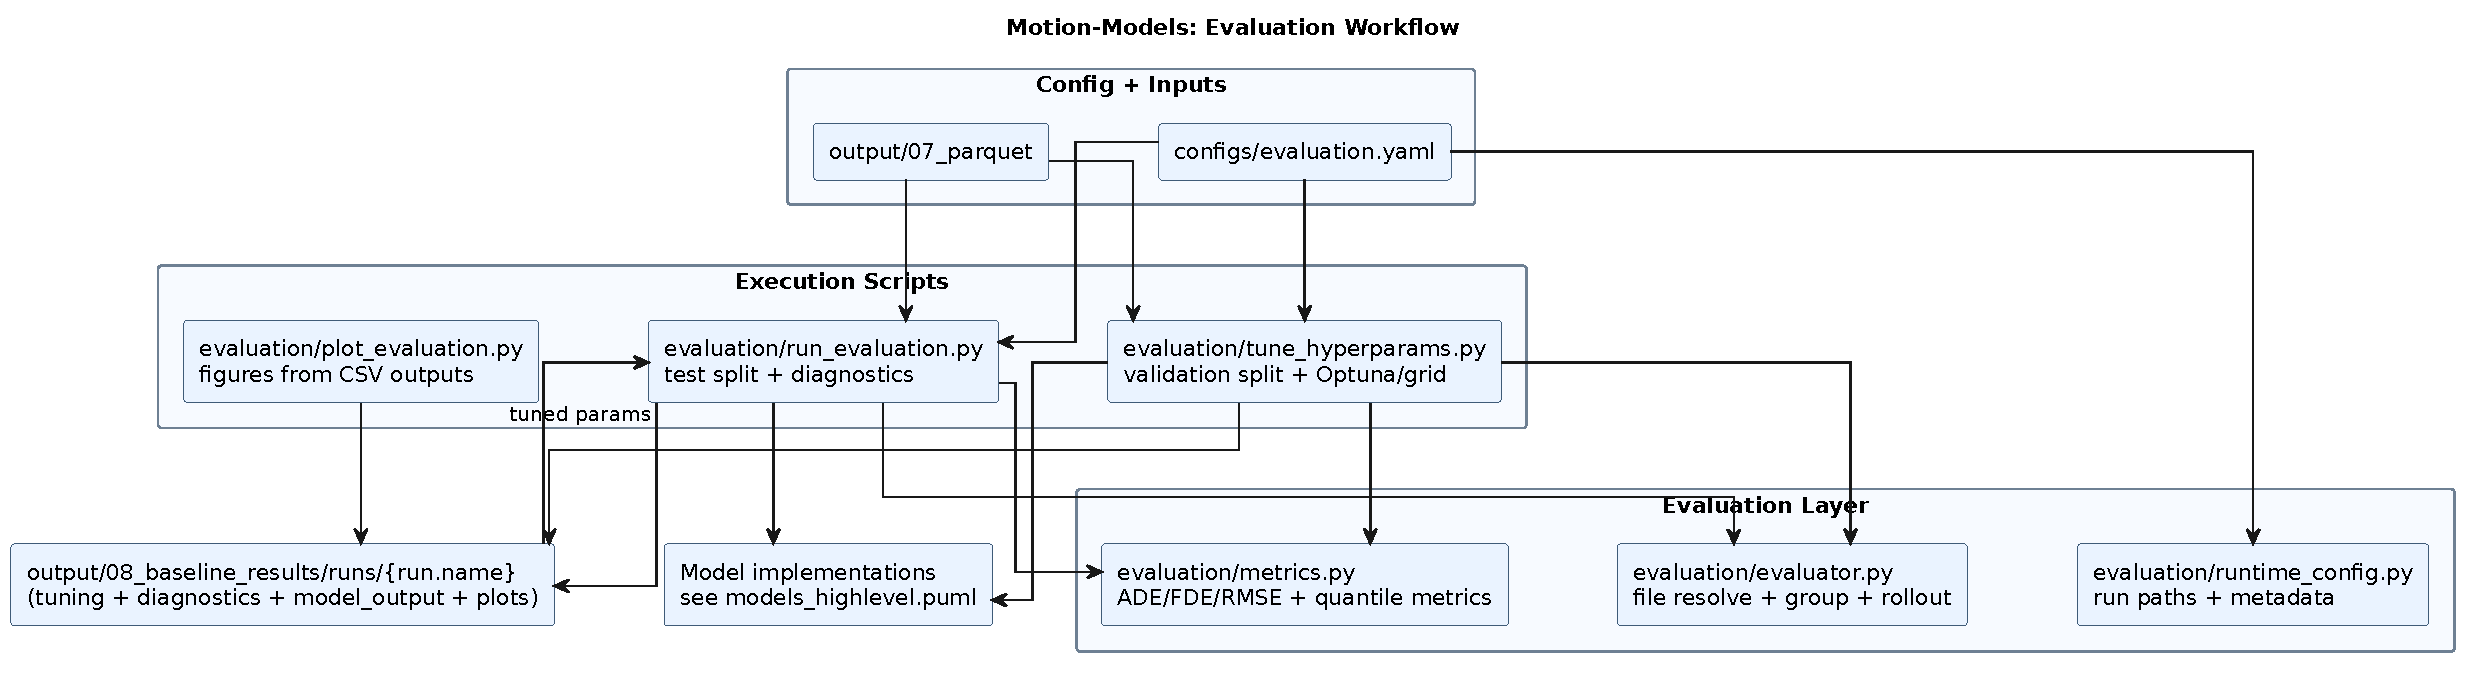
\includegraphics[width=1.18\linewidth, keepaspectratio]{figures/models_evaluation_highlevel.pdf}
    }
    %\caption[Code Overview: Evaluation]{Model Evaluation}
    \caption[Code Overview: Evaluation Workflow]{
        \textbf{Evaluation workflow file and module interactions.}
        The evaluation framework takes two external inputs: the Parquet dataset produced by the preprocessing pipeline (\texttt{output/07\_parquet}) and a YAML configuration file (\texttt{configs/evaluation.yaml}) that specifies enabled models, hyperparameter search spaces, and output paths.
        \texttt{evaluation/runtime\_config.py} resolves run-specific paths and metadata from the configuration.
        \textbf{Tuning} (\texttt{tune\_hyperparams.py}) operates exclusively on the validation split: single-parameter models (CV, CTRV, CTRV Arc, TiRex LSTM) are tuned via exhaustive grid search in parallel worker processes, while multi-parameter models (Hybrid, Kalman, CTRV EKF) are tuned with Optuna TPE.
        Tuning results are written as CSV files under \texttt{output/08\_baseline\_results/runs/\{run.name\}/tuning/}.
        \textbf{Final evaluation} (\texttt{run\_evaluation.py}) reads the tuned parameters and evaluates all enabled models on the test split, writing per-file and per-month diagnostic tables and optional per-model prediction exports to the same run folder.
        Both scripts delegate to \texttt{evaluation/evaluator.py} for file resolution, track grouping, model rollout, and metric aggregation, and to \texttt{evaluation/metrics.py} for computing ADE, FDE, RMSE, and quantile metrics.
        \texttt{evaluation/plot\_evaluation.py} reads the saved CSV outputs to generate all evaluation figures independently of the evaluation runs themselves.
    }
    \label{fig:codeevaluation}
\end{sidewaysfigure}
\clearpage

\begin{comment} dont include it ws
    \chapter{Thesis Advertisement}\begin{figure}
    \centering
    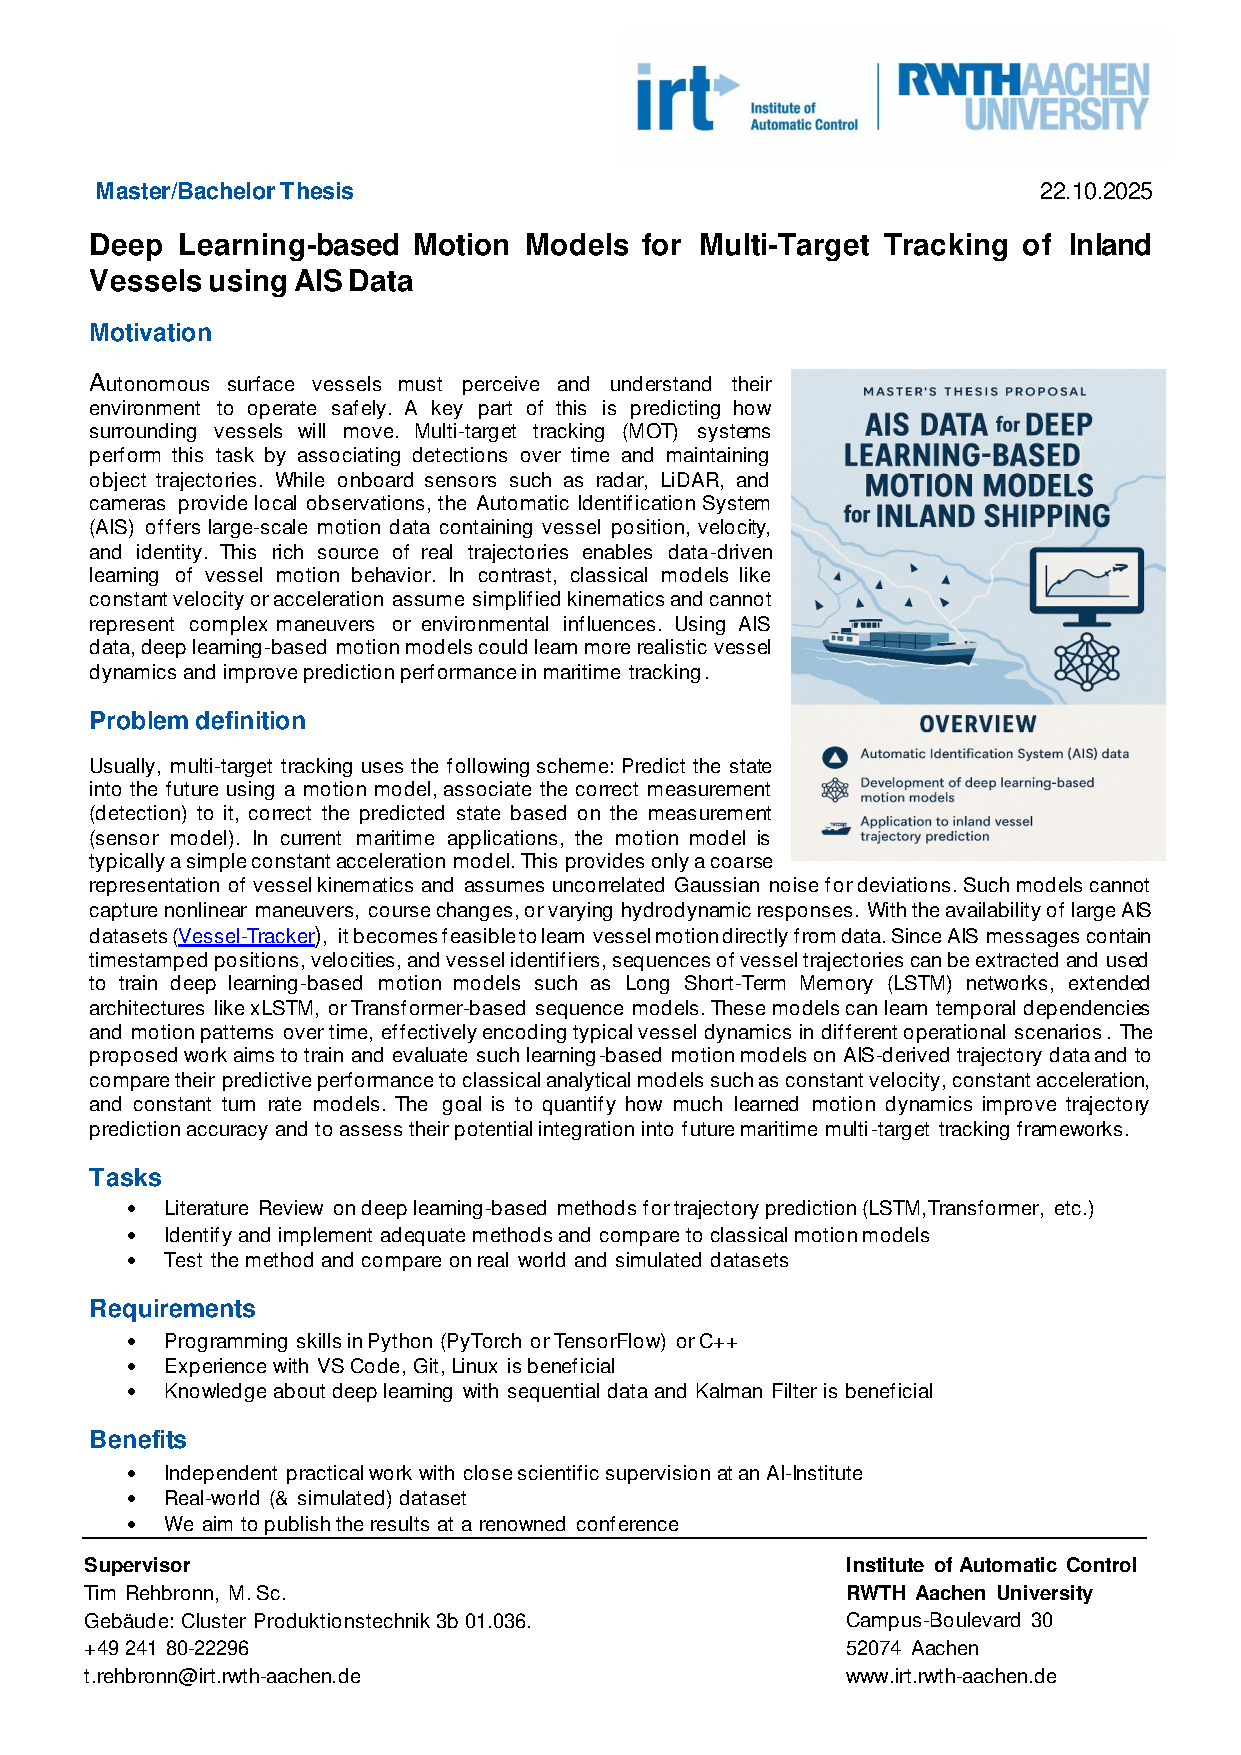
\includegraphics[width=1\linewidth]{ausschreibung_irt.pdf}
    \label{fig:auschschreibung_irt}
\end{figure}

\clearpage
\end{comment}


%\blindtext[5]

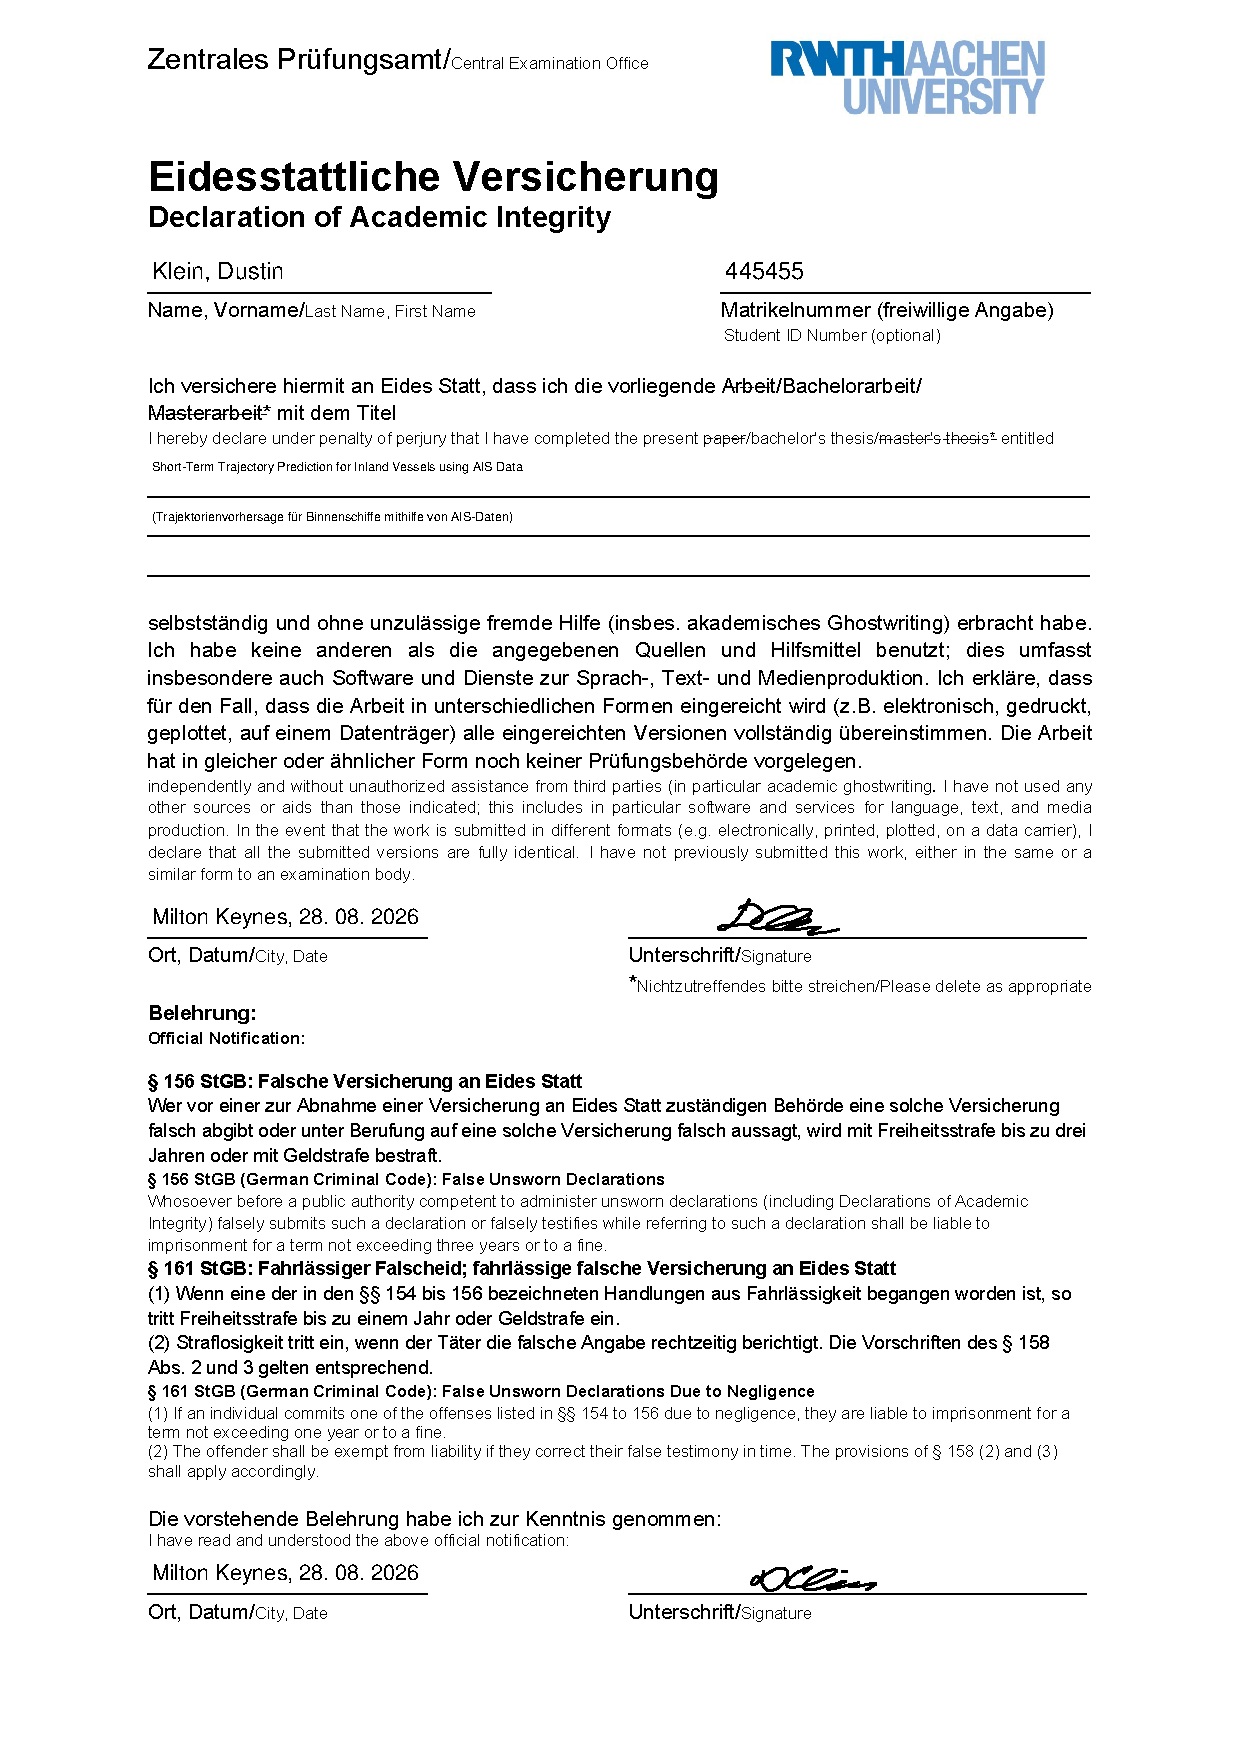
\includepdf[pages=-,pagecommand={},width=\textwidth]{files/oathstatement.pdf}

\end{document}
